\frontmatter
\maketitle


\includegraphics[width=0.25\textwidth]{by-nc-sa}

This work is licensed under the Creative Commons Attribution-NonCommercial-ShareAlike 3.0 United States (\href{https://creativecommons.org/licenses/by-nc-sa/3.0/us/}{CC BY-NC-SA 3.0 US}).  Work has been modified from \href{https://www.ohio.edu/mechanical/thermo/}{{\bf Engineering Thermodynamics - A Graphical Approach} by Israel Urieli} and \href{https://thermo.pressbooks.com/front-matter/letter-to-students/}{{\bf Thermodynamics} by Diana Bairaktarova}.

Modifications include change of format from website to traditional book,
reorganization of multiple chapters,
revised and expanded explanations throughout the book,
updated and revised examples,
recreated and revised figures and plots,
recreation of tables and plots in the Appendices,
addition of multiple homework problems,
and in some cases, omission of parts of the original text.


\tableofcontents

\chapter{Preface}
This work is an attempt to bring high-quality Open Educational Resources to Engineering Thermodynamics at Abilene Christian University, as supported by the Alternative Textbook Initiative Grant.

The goal of Open Educational Resources is to combat the increased cost of textbooks seen in recent years.  Additionally, having resources that are completely free allows students to maintain a library of books, and encourages students to access the book, when they may not have otherwise purchased it.

Another benefit is the ability of the professor to curate exactly what is provided to the student.  Many textbooks are padded with chapters that are skipped in the course, often leading to confusion with homeworks and textbook readings.

Finally, OER allows for collaboration and continuous improvement.  As you work through this text, be on the lookout for things that are confusing, misleading, or simply poorly explained.  Mistakes and errors can be fixed this semester, and any feedback can go into the next version of the book much faster than a traditional publisher.

This text is an adaptation of a web resource originally developed by Dr. Israel Urieli of Ohio University, titled \href{https://www.ohio.edu/mechanical/thermo/}{Engineering Thermodynamics - A Graphical Approach}.  The resource is unique for a number of reasons, the greatest of which being that it is licensed under a \href{https://creativecommons.org/licenses/by-nc-sa/3.0/us/}{Creative Commons license} which allows free sharing and adaptation by other parties.  I should also mention Dr. Diana Bairaktarova, whose adaptation of Dr. Urieli's work was also invaluable in the process of building this version.


\mainmatter

\chapter{Concepts, Dimensions, and Units} \label{ch:intro}
Thermodynamics, generally speaking, is the science of energy. It focuses on the transformation of energy from one form to another.  This includes transforming heat into work, such as in an automobile engine or at a power plant, and transforming work into heat transfer, such as in refrigerators or heat pumps.

The application of Thermodynamics is almost everywhere in our daily life. Examples of some application areas of this subject are: propulsion, internal combustion engines, power plants, refrigeration and air conditioning, solar heating, the interaction of the human body with its surroundings, biomedical devices, the biology of the human body, animals, plants, ecological systems, etc. In this course on thermodynamics we will focus on the analysis of energy systems and the application of these systems to real world contexts.

There are two approaches of teaching Thermodynamics – microscopic and macroscopic. Classical thermodynamics (the macroscopic approach) does not require detailed knowledge of molecular motion to describe a system. Statistical Thermodynamics (the microscopic approach) considers quantum mechanical description of molecules. We will primarily be looking at the macroscopic view, while occasionally using the microscopic approach to improve our basic understanding.

This first chapter is dedicated to introductory concepts, dimensions, and units.
The basic principles of thermodynamics are the conservation of mass, the conservation of energy, and the concept of entropy.  Basic thermodynamics terminology covered in this chapter includes the concepts of a system, properties, states, equilibrium, and processes. 

We will distinguish primary dimensions in Thermodynamics such as mass ($m$), length ($L$), time ($t$), temperature ($T$), electric current ($I$), the amount of a substance ($n$), and secondary (or derived) dimensions such as: velocity ($\frac{\rm m}{\rm s}$), density ($\frac{\rm kg}{\rm m^3}$), pressure ($\frac{\rm N}{\rm m^2}$), etc. In this course we will use the two most prevalent unit systems: the International System of Units (SI) and the United States Customary Units (US), focusing primarily on the first.

%--------------------------------------------------------------------
\section{Thermodynamics and Energy}
%--------------------------------------------------------------------

Thermodynamics is the science of energy, including energy storage and energy in transit. The Conservation of Energy Principle states that energy cannot be created or destroyed, but can only change its form. The three forms of energy storage of greatest interest to us are Potential Energy ({\bf PE}), Kinetic Energy ({\bf KE}), and Internal Energy ({\bf U}), which we introduce below. The two forms of energy in transit that we consider are Work ({\bf W}) and Heat ({\bf Q}), and the interactions between these various forms of energy are defined in terms of the First Law of Thermodynamics.

%--------------------------------------------------------------------
\section{Force and Work}
%--------------------------------------------------------------------
\subsection{Nomenclature}
\begin{center}
\begin{tabular}{cccc}
  Symbol & Meaning & SI Units & English Units \\ \hline 
  $F$ & Force & Newton [N] & pounds-force [lbf] \\
  $m$ & Mass & kilogram [kg] & slugs OR pounds-mass [lbm] \\
  $a$ & Acceleration & $\text{meters}/\text{second}^2$ $[\accSI]$ & $\text{feet}/\text{second}^2$ $[\accE]$ \\
  $W$ & Work & Joules [J] & foot-pounds [ft-lb]
\end{tabular}\\
\end{center}
\subsection{Newton's Second Law}
You should have already seen Newton's Second Law in Engineering Physics.\\

Newton’s Second Law states:
\begin{equation*}
  F = m a
\end{equation*}

Mass ($m$) and force ($F$) are two of the most common dimensions we will be using in this course.  Mass is used in nearly everything, because we are typically using properties of matter given {\bf per unit mass}.  Force is used almost as often, but it tends to be hidden as energy ($F \cdot d = W [{\rm J}]$) or pressure ($F/ A = p\ [{\rm Pa}]$)
%($F [{\rm N}] \cdot d [{\rm m}] = W [{\rm J}]$) or pressure ($F\ [{\rm N}] / A\ [{\rm m^2}] = p\ [{\rm Pa}]$).

You'll notice above that there are two possible units for mass in the US system.  The US unit of slugs is not used from day-to-day, but it is the most direct analog of the SI unit kilograms [kg].  More commonly used is the pound-mass [lbm], which is defined by the amount of mass which creates a pound-force in Earth's standard gravity.\\

Since the acceleration due to gravity g = 32.2$\accE$ we have:
\begin{align*}
  1\:\text{lbf}\:&=32.2\:\accE \cdot 1\:\text{lbm} \\
  1\:\text{lbf}\:&=1\:\accE \cdot 1\:\text{slug} \\
  1\:\text{slug}\:&=32.2\:\text{lbm}
\end{align*}

%Unity Conservation Ratio:

%  \[\frac{N\times s^2}{kg\times m}=1\,\,\,\,\,\text{and}\,\,\,\,\,\frac{lbf\times s^2}{32.174,lbm\times ft}=1\]

\subsection{Work}

We now consider the work done ($W$), which is the energy transferred to an object in motion requiring both an applied force ($F$) and distance moved ($d$). If the force is constant over the distance moved then the work done is given by:
\begin{equation*}
  W=F d,
\end{equation*}

In general, however, the force is not constant over the distance. For varying forces we need to sum all the incremental work processes taking into consideration the variation of the force. This leads to the integral form for determining work done as follows:
\begin{equation*}
  W=\int_0^d F\,dx
\end{equation*}

Notice that the integral form can be simplified to the original form when $F$ is constant.

%--------------------------------------------------------------------
\section{Unit Conversions}
%--------------------------------------------------------------------

It is often necessary to convert data from one unit system to another.  The lists below give conversions for the basic units, along with several shortcuts for commonly used unit combinations.

\begin{multicols}{2}
\subsubsection{Base Units}
\begin{align*}
1 \text{ kg} & = 2.2 \text{ lbm} = 0.0685 \text{ slug} \\
1 \text{ lbm} & = 0.031 \text{ slug} = 0.4536 \text{ kg} \\
1 \text{ N} & = 0.225 \text{ lbf} \\
1 \text{ lbf} &= 4.448 \text{ N} 
\end{align*}

\begin{align*}
1 \text{ m} & = 3.281 \text{ ft} \\
1 \text{ ft} &= 0.3048 \text{ m} \\
1 \text{ cm} &= 0.3937 \text{ in.} \\
1 \text{ in.} &= 2.54 \text{ cm}
\end{align*}

\end{multicols}

\begin{multicols}{2}
\subsubsection{Temperature}
\begin{align*}
T[^{\circ}\text{C}] &= (T[^{\circ}\text{F}]-32^{\circ}\text{F})\cdot 5/9 \\
T[^{\circ}\text{F}] &= T[^{\circ}\text{C}]\cdot 9/5+32^{\circ}\text{F}
\end{align*}

\begin{align*}
T[\text{K}] &= T[^{\circ}\text{C}] + 273.16 \text{K}\\
T[\text{°R}] &= T[^{\circ}\text{F}] + 459.67 \text{°R}
\end{align*}
\end{multicols}

\begin{multicols}{2}
\subsubsection{Energy and Energy Transfer}
\begin{align*}
1 \text{ kJ} & =  737.56 \text{ ft}\cdot \text{lbf} = 0.9478 \text{ BTU} \\
1 \text{ ft}\cdot \text{lbf} & = 1.3558 \text{ J} \\
1 \text{ BTU} & = 778.17 \text{ ft}\cdot \text{ lbf} = 1.055 \text{ kJ}
\end{align*}

\begin{align*}
1 \text{ W} & = 1 \text{ J/s} = 3.41 \text{ BTU/hr}\\
1 \text{ kW} &= 1.341 \text{ hp} = 737.56 \text{ ft}\cdot \text{ lbf/s}\\
1 \text{ hp} &= 550 \text{ ft}\cdot \text{ lbf/s} = 0.7457 \text{ kW} = 2545 \text{ BTU/hr}
\end{align*}

\end{multicols}

\begin{multicols}{2}
\subsubsection{Common Combinations}
\begin{align*}
1 \text{ km/hr} & =  0.6214 \text{ mile/hr} = 0.2778 \text{ m/s} \\
1 \text{ mile/hr} & =  1.609 \text{ km/hr} = 1.467 \text{ ft/s} \\
1 \text{ kPa} & = 0.145 \text{ lbf/in}^2 = 0.021 \text{ lbf/ft}^2 \\
1 \text{ atm} & = 101.325 \text{ kPa} = 14.7 \text{ lbf/in}^2 \\
1 \text{ lbf/in}^2 &= 6.895 \text{ kPa} = 144 \text{ lbf/ft}^2
\end{align*}

\begin{align*}
1 \text{ m}^3 &= 1000 \text{ L} = 35.315 \text{ ft}^3 = 264.2 \text{ gal}\\
1 \text{ cm}^3 &= 0.061 \text{ in}^3 \\
1 \text{ in}^3 &= 16.39 \text{ cm}^3 \\
1 \text{ L} &= 10^{-3} \text{ m}^3 = 0.0353 \text{ ft}^3 = 0.264 \text{ gal} \\
1 \text{ gal} &= 0.00378 \text{ m}^3 = 0.1337 \text{ ft}^3 = 3.78 \text{ L}
\end{align*}

\end{multicols}

%\subsubsection{Example 1.1}
\begin{example}{Unit Conversion}
Figure \ref{fig:ch1_speedometer} shows a speedometer.  You can see that 50 mph is approximately the same as 80 km/h.  How much error is present in that estimate?

\begin{enumerate}
\item Determine the approximate conversion created by the above information. Compare that to the value given in the Common Combinations section above.
\item Use the base unit conversions, along with 1 mile = 5280 feet and 1 hour = 3600 seconds to recreate the conversion value.
\end{enumerate}
\begin{center}
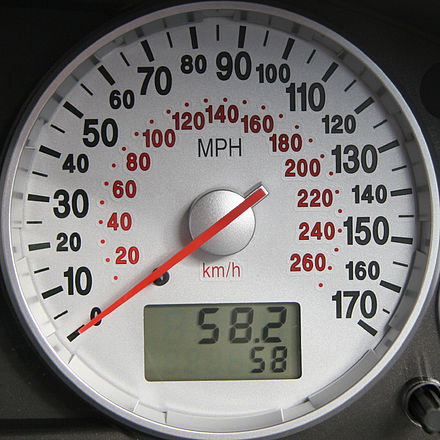
\includegraphics[width=0.5\textwidth]{speedometer}
\captionof{figure}{An old Ford speedometer.  From \href{https://commons.wikimedia.org/wiki/File:Ford_Mondeo_MK3_ST220_-_Speedometer.jpg}{Wikimedia Commons}.}
\label{fig:ch1_speedometer}
\end{center}
\begin{enumerate}
\item The Common Combinations section gives the conversion ``$1 \text{ mile/hr} =  1.609 \text{ km/hr}$''.  We can create a similar equation from the speedometer, as shown below:
\begin{equation*}
50 \frac{\text{mile}}{\text{hr}} = 80 \frac{\text{km}}{\text{hr}}
\end{equation*}
At this point, it's simple to create a similar conversion to the one given:
\begin{align*}
\frac{1}{50}50 \frac{\text{mile}}{\text{hr}} &= \frac{1}{50}80 \frac{\text{km}}{\text{hr}}\\
1 \frac{\text{mile}}{\text{hr}} &= 1.6 \frac{\text{km}}{\text{hr}}
\end{align*}

This is less than 1\% off from the more accurate value given.

\item In order to build a conversion from base units, we need our starting point (1 mph), and fix one unit at a time.
\begin{align*}
1 \frac{\text{mile}}{\text{hr}} \cdot \frac{5280 \text{ ft}}{1\text{ mile}} &= 5280 \frac{\text{ft}}{\text{hr}} \\
5280 \frac{\text{ft}}{\text{hr}} \cdot \frac{1\text{ m}}{3.281 \text{ ft}} &= 1609.3 \frac{\text{m}}{\text{hr}} \\
1609.3 \frac{\text{m}}{\text{hr}} \cdot \frac{1 \text{ km}}{1000 \text{ m}} &= 1.6093 \frac{\text{km}}{\text{hr}}
\end{align*}
We get a final result which is actually more accurate than the value given in the earlier list.
\end{enumerate}
\end{example}

Outside of an exam or quiz, it is always good to double-check unit conversions with values found online.  Typing \href{https://www.google.com/search?q=1+mph+in+kmph}{``1 mph in kmph'' into Google} pulls up a very useful unit conversion tool.

%--------------------------------------------------------------------
\section{Forms of Energy} \label{sec:ch1_energyForms}
%--------------------------------------------------------------------
The various forms of energy of interest to us are introduced in terms of a solid body having a mass m [kg]. These include potential, kinetic and internal energy.

\subsection{Potential Energy}
Potential energy (PE) is associated with the elevation of the body, and can be evaluated in terms of the work done to lift the body from one datum level to another under a constant acceleration due to gravity $g\left[\accSI\right]$, as follows:

\begin{equation}
  W=\int_{h_1}^{h_2}F\,dx=\int_{h_1}^{h_2}m\cdot g\,dx=m\cdot g(h_2-h_1)=m\cdot\Delta pe=\Delta PE
\end{equation}

Typically, we simplify this to say that $PE = mgh$.

\subsection{Kinetic Energy}
Kinetic energy (KE) of a body is associated with its velocity $V\left[\velSI\right]$ and can be evaluated in terms of the work required to change the velocity of the body, as follows:
\begin{equation}
  W=\int F\,dx=\int m\cdot a \,dx=\int m\cdot\frac{dV}{dt}dx
\end{equation}
however, velocity $V=\frac{dx}{dt}$, thus integrating from $V_1$ to $V_2$:
\begin{equation}
  W=\int_{V_1}^{V_2}m\cdot V\,dV=m\cdot\left(\frac{V_2^2-V_1^2}{2}\right)=m\cdot\Delta ke=\Delta KE
\end{equation}
Typically, this is simplified to say that $KE = \frac{1}{2} m V^2$.

\subsection{Internal Energy} \label{sec:ch1_internalEnergy}

Internal energy (U) of a body is that associated with the molecular activity of the body as indicated by its temperature T [°C], and can be evaluated in terms of the heat required to change the temperature of the body having a specific heat capacity  $c\left[\frac{\rm J}{\rm kg \cdot°C}\right]$, as follows:
\begin{equation}
  Q=m\cdot c\cdot\Delta T=m\cdot\Delta u=\Delta U
\end{equation}

Unfortunately, the specific heat $c$ changes with temperature.  For this reason, it is typically necessary to look up the internal energy of a substance from a table.

\begin{example}{Cooking with Internal Energy}

In order to gain an intuitive appreciation for the relative magnitudes of the different forms of energy we consider the (tongue-in-cheek) example of an attempt to cook a turkey by potential energy. The turkey is brought to the top of a 100 m building (about 30 stories) and then dropped from the ledge. The potential energy is thus converted into kinetic energy, and finally on impact the kinetic energy is converted into internal energy. The increase in internal energy is represented by an increase in temperature, and hopefully, if this experiment is repeated enough times the temperature increase will allow the turkey to cook. This remarkable experiment was first reported by R.C.Gimmi and Gloria J Browne – “Cooking with Potential Energy“, published in the Journal of Irreproducible Results (Vol. 33, 1987, pp 21-22).

Potential Energy
\begin{equation*}
W=\int_0^h F \ \mathrm{d}x = \int_0^h m g \ \mathrm{d}x
\end{equation*}

\begin{equation*}
\color{red}\boxed{\color{black}W=m\cdot g \cdot h=\Delta PE}
\end{equation*}

Internal Energy

\begin{equation*}
%\color{red}\boxed{\color{black}Q=m \cdot C \cdot \Delta T = \Delta U}
\redbox{Q=m \cdot C \cdot \Delta T = \Delta U}
\end{equation*}

Kinetic Energy
  \begin{align*} W &= \int F \ \mathrm{d}x = \int mg \ \mathrm{d}x = \int m \frac{\mathrm{d}{V}}{\mathrm{d}t} \ \mathrm{d}x \\ &= m \int \frac{\mathrm{d}x}{\mathrm{d}t} \ \mathrm{d}{V} = m \int_0^{{V}} {V} \ \mathrm{d}{V} \end{align*}

\begin{equation*}
  \color{red}\boxed{\color{black}W=\frac{m \cdot {V}^2}{2}=\Delta KE}
\end{equation*}

Equating all three energy forms:
\begin{equation*}
\Delta PE = \Delta KE = \Delta U \ [\rm J]
\end{equation*}

\begin{equation*}
m \cdot g \cdot h=\frac{m \cdot {V}^2}{2} = m \cdot C \cdot \Delta T
\end{equation*}

Since mass m is common, evaluate specific energy (h=100 m):
\begin{equation*}
\Delta pe = \Delta ke = \Delta u \ [\frac{\rm J}{\rm kg}]
\end{equation*}

\begin{equation*}
g \cdot h = \frac{{V}^2}{2} = C \cdot \Delta T \approx 1000 \ [\frac{\rm J}{\rm kg}]
\end{equation*}

\begin{equation*}
\frac{{V}^2}{2} \left[\frac{\rm m^2}{\rm s^2}\right] =
1000 \left[ \frac{\rm J}{\rm kg} \cdot
\left(\frac{\rm N \cdot m}{\rm J}\right) \cdot \left(\frac{1}{\rm N} \frac{\rm kg \cdot m}{\rm s^2} \right)\right]
\end{equation*}

\begin{equation*}
{V}_{\text{impact}} = \sqrt{2000} = 44.7 \left[ \frac{\rm m}{\rm s}\right] (\approx 100 \ \rm mph !)
\end{equation*}

We estimate the specific heat of a turkey.
\begin{equation*}
c = 3000 \ [{\rm J / kg ^{\circ}C}] (\text{a little less than water})
\end{equation*}

Thus
\begin{equation*}
c \Delta T = 3000 \ \Delta T = 1000 \ [{\rm J / kg}] \implies \color{red}\boxed{\color{black} \Delta T = 0.33 ^{\circ}C}
\end{equation*}

What a disappointment! At 0.33°C per fall it will require repeating the experiment 600 times just to reach the cooking temperature of 200°C.

\end{example}

%--------------------------------------------------------------------
\section{Basic Properties of Matter}
%--------------------------------------------------------------------
\subsection{Nomenclature}
\begin{tabular}{cccc}
  Symbol & Meaning & SI Units & English Units \\ \hline 
  $\rho$ & Density & $\text{kg}/\text{m}^3$ & $\text{slug}/\text{ft}^3$ OR $\text{lbm}/\text{ft}^3$ \\
  $p$ & Pressure & Pascal [Pa] & $\text{pounds}/\text{foot}$ [psf] \\
  $v$ & Specific Volume & $\text{m}^3/\text{kg}$ & $\text{ft}^3/\text{slug}$ OR $\text{ft}^3/\text{lbm}$ \\
  $T$ & Temperature & °C OR K & °F OR °R
\end{tabular}\\
\subsection{Density}
Density is the amount of mass in a given volume.  If the density is constant throughout the volume, we can say that $m = \rho \cdot {\rm Vol}$.  The units used for density are composed of a unit of mass, such as kg, and a unit of volume, such as $\rm m^3$.

The density of air under standard atmospheric conditions is around $1.2\ {\rm kg/m^3}$.  The density of water in normal conditions is about $1000\ {\rm kg/m^3}$.  Many solids have higher densities still.

\subsection{Specific Volume}
In Thermodynamics, we often prefer to use {\bf mass-specific} properties.  Mass-specific simply means that a property is given per unit mass.  Density is unfortunately volume-specific, rather than mass-specific.  In order to convert density to a mass-specific property, we simply need to invert it.  Specific volume is the result: $v = 1/\rho$, represented in $\rm m^3/kg$.

\subsection{Pressure}
Gases and liquids (together referred to as fluids) both push on all surfaces they touch.  The force they apply is based on their pressure.  If pressure is constant over the surface, we can say that $F = p\cdot A$.  A more in-depth study of this phenomenon is covered in Fluid Mechanics.

The basic unit of pressure is the Pascal [Pa], which is identical to a Newton per square meter $\left[\frac{\rm N}{\rm m^2}\right]$.  However, practical units are kilopascal [kPa], bar [100 kPa] or atm (atmosphere) [101.32 kPa]. The {\bf gauge} (or {\bf vacuum}) pressure is related to the {\bf absolute} pressure as shown in the diagram below:

\begin{figure}[H]
\centering
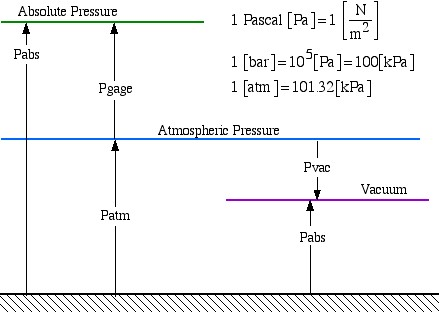
\includegraphics[width=0.75\textwidth]{Pressure}
\caption{Various pressure measurements.  Gauge and vacuum pressure are measured compared to atmosphere.}
\label{fig:ch1_pressure}
\end{figure}

The basic method of measuring pressure is by means of a {\bf manometer}, as shown below:

\begin{figure}[H]
\centering
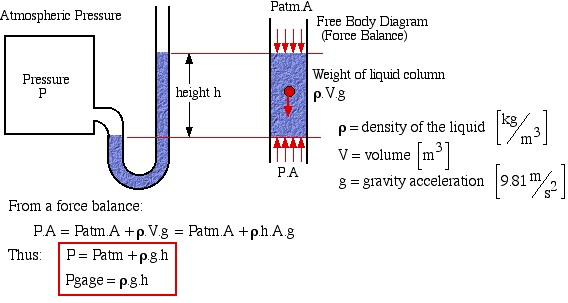
\includegraphics[width=0.75\textwidth]{Manometer}
\caption{A diagram of a manometer, which is used to find the pressure difference between two fluids.}
\label{fig:ch1_manometer}
\end{figure}

The basic principle here is that the force caused by excess pressure on one side is balanced by the extra weight of fluid on the other side.  You can find the difference in pressure through the formula $\Delta p = \rho g \Delta h$.  In this case, $\Delta p = p - p_{atm}$.

Manometers can only measure pressure differences, meaning that they are useful for gauge and vacuum pressures, but not for finding absolute or atmospheric pressure.

In order to find atmospheric pressure (and by extension, absolute pressure), a mercury {\bf barometer} can be used as follows:

\begin{figure}[H]
\centering
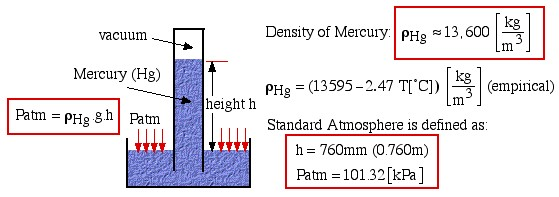
\includegraphics[width=0.75\textwidth]{Barometer}
\caption{A diagram of a barometer, which is used to find the absolute pressure of a fluid.}
\label{fig:ch1_barometer}
\end{figure}

The key here is the vacuum above the mercury.  For a pure vacuum, absolute pressure is 0.  With that knowledge, the barometer works the same as the manometer above, with $\Delta p = p_{atm} - 0$.

\subsection{Temperature}
Temperature is a measure of molecular activity, and a temperature difference between two bodies in contact (for example the immediate surroundings and the system) is the driving force leading to heat transfer between them.

Both the Fahrenheit and the Celsius scales are in common usage in the US, hence it is important to be able to convert between them. Furthermore we will find that in some cases we require the Absolute (Rankine and Kelvin) temperature scales (for example when using the Ideal Gas Equation of State).

To explain the difference between Fahrenheit and Celsius, remember that Fahrenheit describes how hot something is to a human (0 being very cold, and 100 being very hot).  Celsius does the same for water (0 being freezing, and 100 being boiling).  Rankine uses the Fahrenheit scale, but sets the zero point at absolute zero (0°R = -459.67°F).  Kelvin does the same, but for Celsius (0 K = -273.15°C).

%--------------------------------------------------------------------
\section{Types of Thermodynamic Systems}
%--------------------------------------------------------------------

For purposes of analysis we consider two types of thermodynamic systems: closed systems and open systems.

\subsection{Closed Systems}
Closed systems are usually referred to as {\bf control masses}. This type of system is separated from its surroundings by a physical boundary. Energy in the form of {\bf work} or {\bf heat} can flow across the system boundary, however there can be no mass flow across the boundary. One typical example of a system is a piston/cylinder device in which the system is defined as the fixed mass of fluid contained within the cylinder.

\begin{figure}[H]
\centering
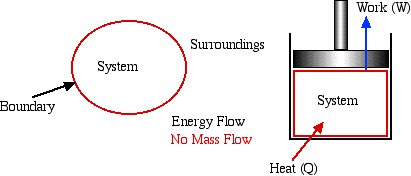
\includegraphics[width=0.5\textwidth]{ClosedSystem}
\caption{A closed system allows energy flow, but no mass flow.}
\label{fig:ch1_closedSystem}
\end{figure}

A closed system that additionally restricts energy flow is known as an {\bf isolated system}.  An isolated system will always have the same amount of mass and energy that it started with.

\subsection{Open Systems}
Open Systems are usually referred to as {\bf control volumes}. In this case, in addition to work or heat, we have mass flow of the working fluid across the system boundaries through inlet and outlet ports. In this course we will be exclusively concerned with {\bf steady flow} control volumes, in that the net mass of working fluid within the system boundaries remains constant (i.e. mass flow in = mass flow out). The following sections refer mainly to systems – we will consider control volumes in more detail starting with Chapter 4.


\begin{figure}[H]
\centering
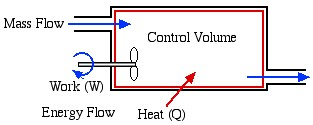
\includegraphics[width=0.5\textwidth]{OpenSystem}
\caption{An open system allows both energy flow and mass flow.}
\label{fig:ch1_openSystem}
\end{figure}

%--------------------------------------------------------------------
\section{Intensive and Extensive Properties}
%--------------------------------------------------------------------

Systems are defined by the properties of the matter that make them up.  For instance, you can define a piston by the total amount of mass inside, the temperature, the pressure, etc.  A large part of Thermodynamics is defining and calculating the properties of matter.

Properties can be either {\bf extensive} or {\bf intensive}.  Extensive properties depend on the ``extent'' of the system, meaning that if you have more mass in the system, you will have more of the property.  Key examples of this are volume and mass, though you can define any of the energies as extensive.  Intensive properties are independent of the size of the system.  Pressure and temperature are key examples, though most properties can be redefined as intensive. For instance, density ($\rho$) and specific volume ($v$) are both intensive properties defined from extensive properties.

Another example is the specific internal energy ($u$), which is simply the total internal energy ($U$) divided by mass:

\begin{equation*}
u \left[\frac{\rm kJ}{\rm kg}\right] = \frac{U\ [{\rm kJ}]}{m\ [{\rm kg}]}
\end{equation*}

In general, a {\bf specific} property is an intensive property which has been obtained by dividing the extensive property by the mass of the system.

%--------------------------------------------------------------------
\section{State and Equilibrium} \label{sec:states}
%--------------------------------------------------------------------

The {\bf state} of a system is defined by the values of the various intensive properties of the system.

The {\bf state postulate} states that if two independent intensive property values are defined, then all the other intensive property values (and thus the state of the system) are also defined. This can significantly simplify the graphical representation of a system, since only two-dimensional plots are required. Note that pressure and temperature are not necessarily independent properties, thus a boiling liquid will change its state from liquid to vapor at a constant temperature and pressure.

We assume that throughout the system {\bf equilibrium} conditions prevail, which means that there are no temperature or pressure gradients or transient effects. At any instant the entire system is under chemical and phase equilibrium, meaning that all chemical reactions and phase transitions (such as boiling) happen instantly, with no time delay.  An alternative viewpoint is that any processes (see Section \ref{sec:ch1_process}) happen slowly enough that any chemical reactions or phase transitions have a chance to complete as we inch along.

Note that this is an assumption, and that in future classes, such as Heat and Mass Transfer, you will be interested in those gradients.


%--------------------------------------------------------------------
\section{Process and Cycle} \label{sec:ch1_process}
%--------------------------------------------------------------------

A {\bf process} is a change of state of a system from an initial to a final state due to an energy interaction (work or heat) with its surroundings. For example in the following diagram the system has undergone a compression process in the piston-cylinder device.

\begin{figure}[H]
\centering
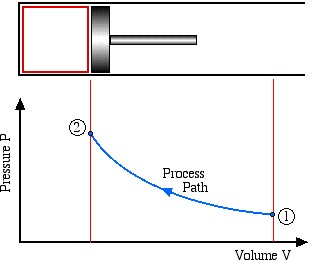
\includegraphics[width=0.5\textwidth]{BasicPistonProcess}
\caption{A compressing piston increases pressure and reduces volume in a system.}
\label{fig:ch1_process}
\end{figure}

The {\bf process path} defines the type of process undergone. Typical process paths are:
\begin{itemize}
\item Isothermal (constant temperature process)
\item Isochoric or Isometric (constant volume process)
\item Isobaric (constant pressure process)
\item Adiabatic (no heat flow to or from the system during the process)
\end{itemize}

We assume that all processes are {\bf quasi-static} in that equilibrium is attained after each incremental step of the process.

A system undergoes a {\bf cycle} when it goes through a sequence of processes that leads the system back to its original state.

% --------------------------------------------------------------------
\section{Using Software: Google Colab (Python)} \label{sec:ch1_colab}
% --------------------------------------------------------------------
\href{https://colab.research.google.com}{Google Colab} is a free IDE (integrated development environment) for Python.  Through Colab, you can write Python code, link to countless existing libraries of code and data, and run the code you write.

\subsection{Setup and CoolProp Basics}
To start off, click the link above (or search Google for ``Google Colab'').  You want to create a New Notebook, so either select the option from the pop-up menu, or select ``File'' from the menu bar and click on ``New notebook''.

Your empty notebook should look something like Figure \ref{fig:ColabScreenshot1}.

\begin{figure}[H]
\centering
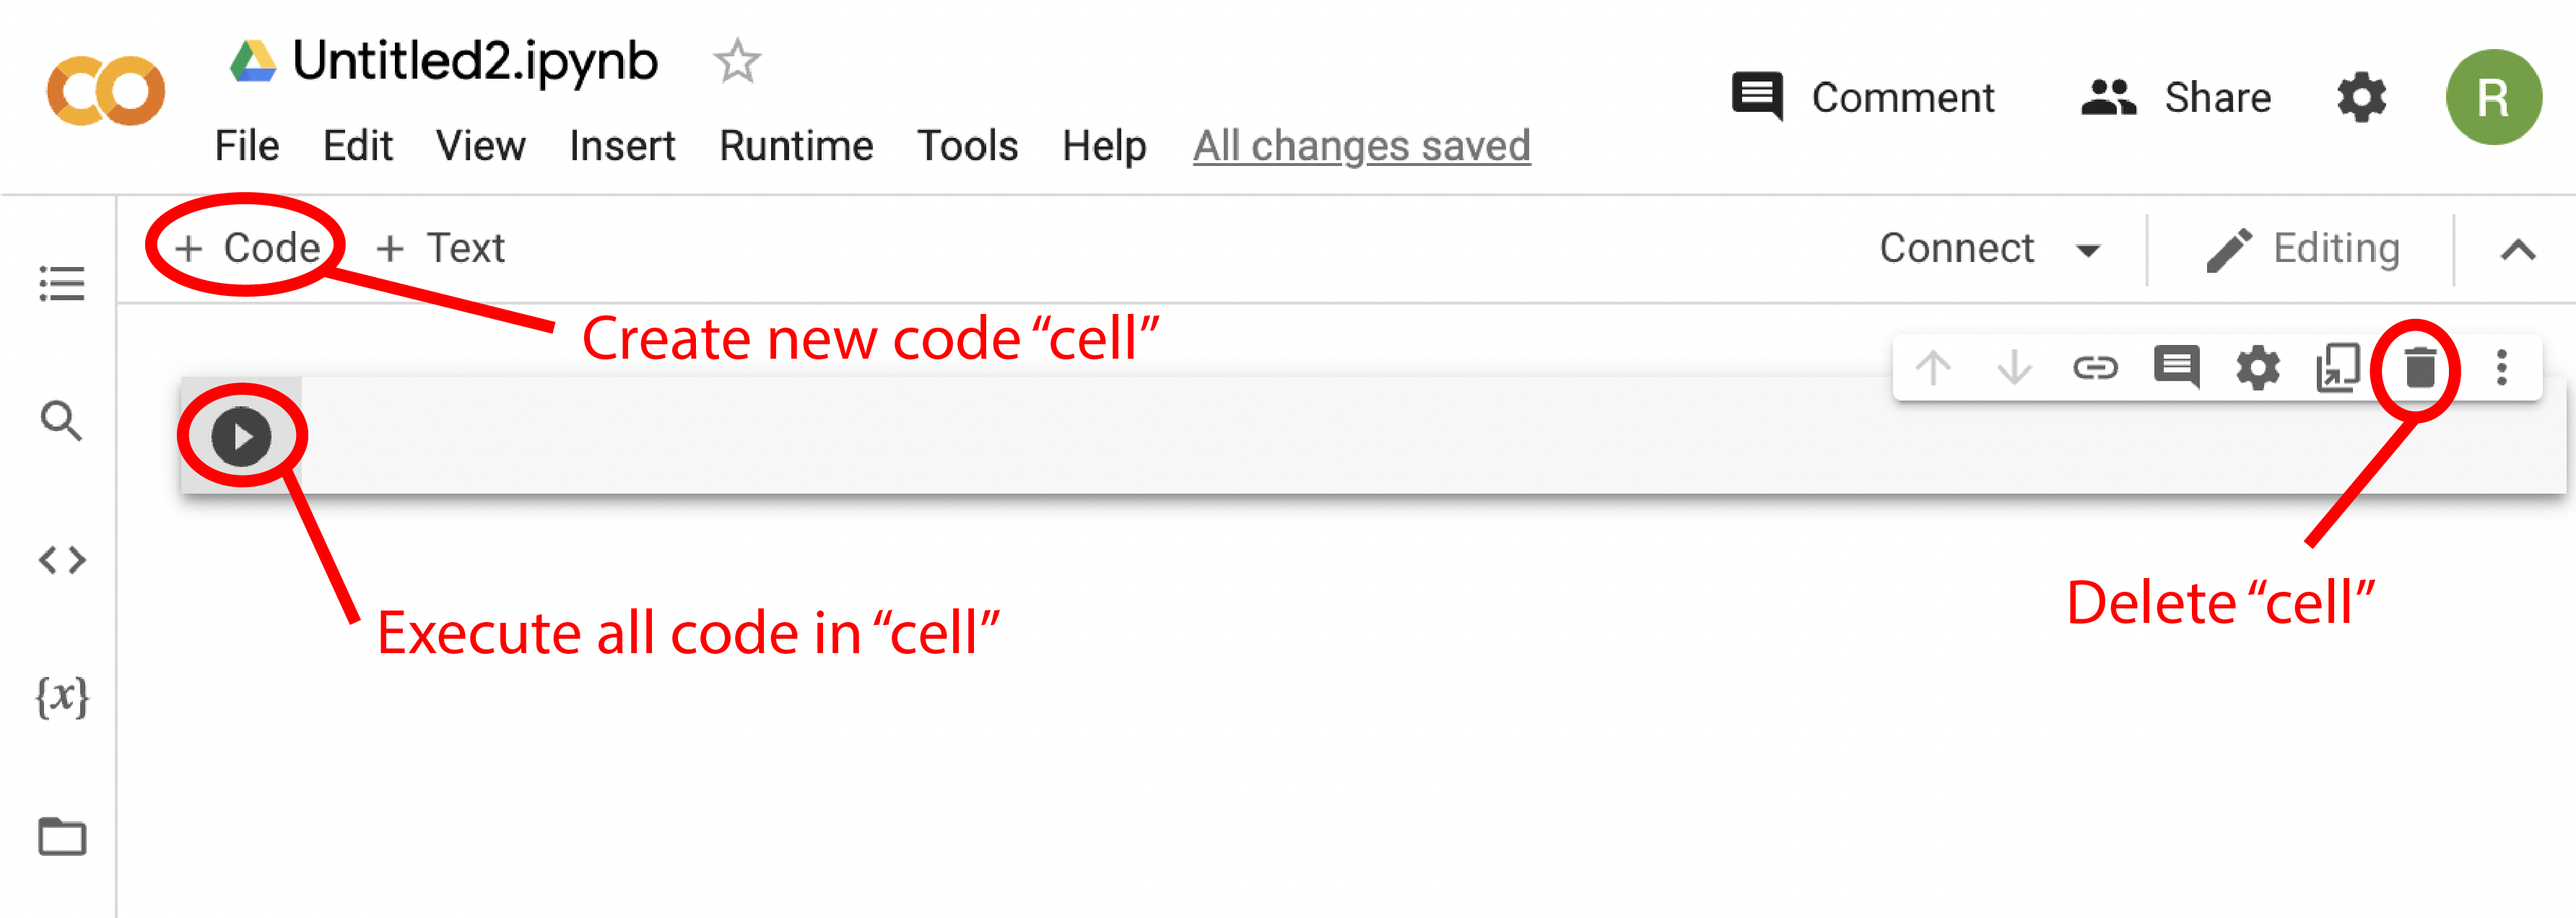
\includegraphics[width=0.9\textwidth]{ColabScreenshot1_labelled}
\caption{An empty notebook in Google Colab, with several important buttons labeled.}
\label{fig:ColabScreenshot1}
\end{figure}

Once you have your notebook created, we need to start off with some commands to link to some common libraries:

\begin{Verbatim}[commandchars=\\\{\}]
\textcolor{OliveGreen}{# Clear all variable definitions}
\textcolor{blue}{\%reset} -f                         
\textcolor{violet}{from} numpy \textcolor{violet}{import} *               \textcolor{OliveGreen}{# Import common numerical functions (like sqrt)}
\textcolor{violet}{from} matplotlib.pyplot \textcolor{violet}{import} *   \textcolor{OliveGreen}{# Import plotting functions (like plot)}
\end{Verbatim}

Everything to the right of the \# symbol is a comment (text that is ignored by Python).  Comments are not part of the code, but are helpful in describing the code in plain language.

The \texttt{reset} command removes variable definitions, and essentially makes sure we're working from a clean slate.  Some of the most frustrating errors to debug stem from the fact that something is defined in a way that you aren't expecting, and this helps avoid some of those errors.

The \texttt{from ... import *} command grabs all of the functions from a library and gives us access to them.  We are getting function from the \texttt{numpy} library and the \texttt{matplotlib} library.  The \texttt{numpy} library contains functions like \texttt{sqrt}, \texttt{sin}, and \texttt{log}, and generally allows you to do everything you could do on a scientific calculator (plus a lot more we won't talk about here).  The \texttt{matplotlib} library gives you access to \texttt{plot} and all the functions you need to make plots look good.

\subsection{Basic Math} \label{sec:pythonBasics}

Let's say that we know the area of a square (in acres) and would like to find out the length of one of the sides.  We can make this happen through the following lines of code:

\begin{Verbatim}[commandchars=\\\{\}]
areaInAcres = \textcolor{JungleGreen}{2.5}  \textcolor{OliveGreen}{# 2.5 acres}
areaInSqFt = areaInAcres*\textcolor{JungleGreen}{43560}  \textcolor{OliveGreen}{# conversion to square feet}
sideLength = sqrt(areaInSqFt)   \textcolor{OliveGreen}{# Area = length^2}
\end{Verbatim}

This will convert from acres to square feet, then take the square root in order to find the length of one of the sides.  Running this code will not produce any errors, but at the same time, it won't seem to do anything.

In order to get information out of the code, we need to use the \texttt{print} command.  The simplest form is shown below:
\begin{Verbatim}[commandchars=\\\{\}]
print(sideLength)
\end{Verbatim}
This will output the numerical value of \texttt{sideLength}, but nothing else.  The problem with this arises when you are printing several different values over the course of your code.  It becomes very easy to forget which number is which, or at the very least waste time trying to figure it out.

What I prefer is a slightly more complicated version that includes a label and units:
\begin{Verbatim}[commandchars=\\\{\}]
print(\textcolor{purple}{'length = '}, sideLength, \textcolor{purple}{'m'})   
\end{Verbatim}

The little bit of up-front effort means that you are less likely to forget what the number means in the future.

\subsection{Plotting in Python}

In order to make a plot, we first need to accumulate some data.  The easiest way of doing this is to manually build a {\bf list}.  Once you have two lists, you can plot!  You can do this with the following three lines of code:
\begin{Verbatim}[commandchars=\\\{\}]
X = [0, 1, 2, 3, 4]
Y = [4, 1, 0, 1, 4]
plot(X,Y)
\end{Verbatim}

After running, you should end up with a screen that looks like Figure \ref{fig:ColabScreenshot2}

\begin{figure}[H]
\centering
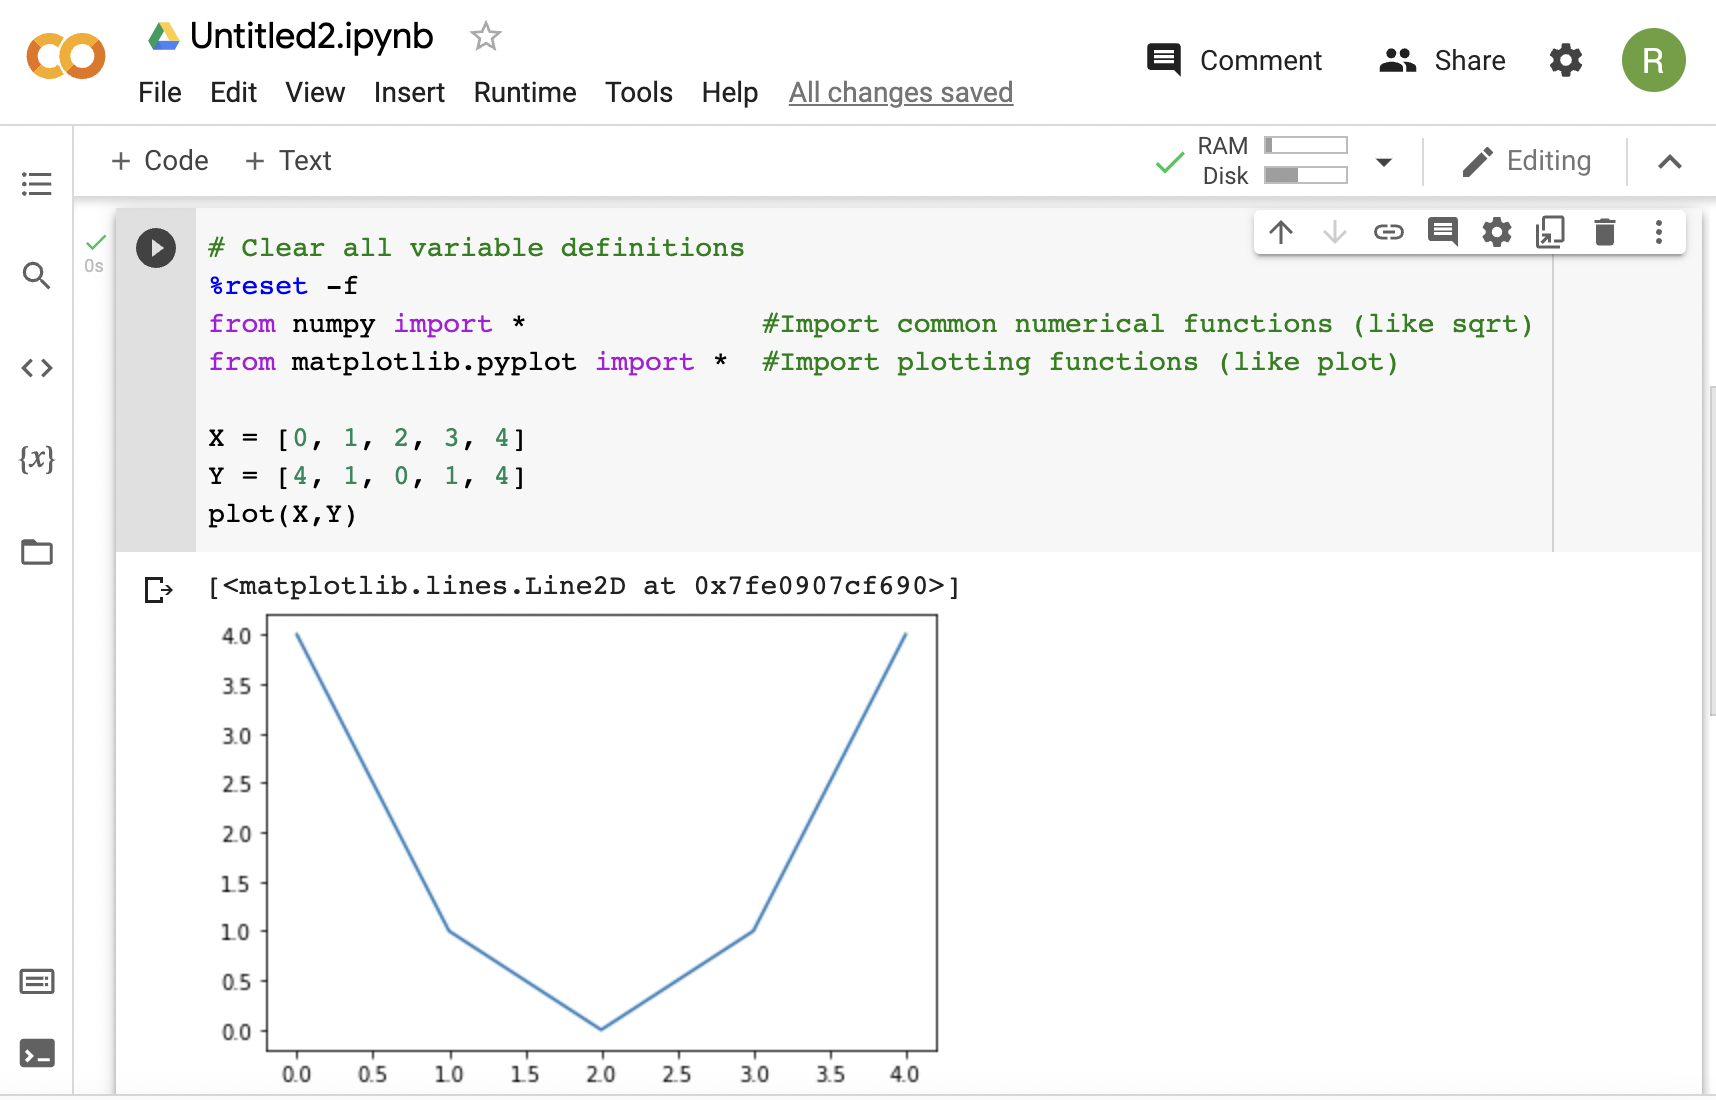
\includegraphics[width=0.9\textwidth]{ColabScreenshot2}
\caption{Google Colab, displaying a simple plot.}
\label{fig:ColabScreenshot2}
\end{figure}

We could give labels, titles, etc., but there's not much point when our data doesn't actually mean anything.  Instead, let's return to our original problem of find the side length of a plot of land.

In order to attack this problem, we will build a list and calculate our side length values all at once.  To start, we need to define all of the areas we want to work with.  Instead of manually putting those in a list, we will use the \texttt{linspace} command:

\begin{Verbatim}[commandchars=\\\{\}]
areaInAcres = linspace(0, 25, 100) \textcolor{OliveGreen}{# create 100 points between 0 and 25}
\end{Verbatim}
\texttt{linspace} has three {\bf arguments}, or input values.  The first and second define the beginning and ending points of the list, respectively.  The last argument is the number of points.  If you want to see all the values in the list, you can use the command \texttt{print(areaInAcres)}.

Python can actually work with lists for most simple functions (like multiplication, \texttt{sqrt}, trig functions, etc.).  This means we can re-use the code we wrote for Section \ref{sec:pythonBasics}:

\begin{Verbatim}[commandchars=\\\{\}]
areaInAcres = linspace(0, 25, 100) \textcolor{JungleGreen}{2.5}  \textcolor{OliveGreen}{# 2.5 acres}
areaInSqFt = areaInAcres*\textcolor{JungleGreen}{43560}  \textcolor{OliveGreen}{  # conversion to square feet}
sideLength = sqrt(areaInSqFt)   \textcolor{OliveGreen}{  # Area = length^2}
\end{Verbatim}

Then, we can plot \texttt{areaInAcres} as the x-axis, and \texttt{sideLength} as the y-axis.

\begin{Verbatim}[commandchars=\\\{\}]
plot(areaInAcres, sideLength)
\end{Verbatim}

This will give us a plot, but since our line actually has meaning, we should give the plot labels and a title.  While we're at it, we'll also modify the axes and add grid lines.

The label and title commands are very straightforward.  The important thing to note is that the arguments must be {\bf strings}, which are collections of characters.  You denote a string using quotation marks.

\begin{Verbatim}[commandchars=\\\{\}]
xlabel(\textcolor{purple}{'Plot Area [ac]'})
ylabel(\textcolor{purple}{'Side Length [m]'})
title(\textcolor{purple}{'Length of Side of Land vs. Acreage'})
\end{Verbatim}

Next, we'll use the \texttt{axis} command.  \texttt{axis} takes a list of values as an argument, which should be in the order \texttt{[<xmin>, <xmax>, <ymin>, <ymax>]}.  We'll implement this as follows:
\begin{Verbatim}[commandchars=\\\{\}]
axis([0, 25, 0, 1200])
\end{Verbatim}

Finally, let's add some grid lines to make data a little easier to extract.
\begin{Verbatim}[commandchars=\\\{\}]
grid(visible=True)
\end{Verbatim}

When you've put everything together, Colab should look like Figure \ref{fig:ColabScreenshot3}.

\begin{figure}[H]
\centering
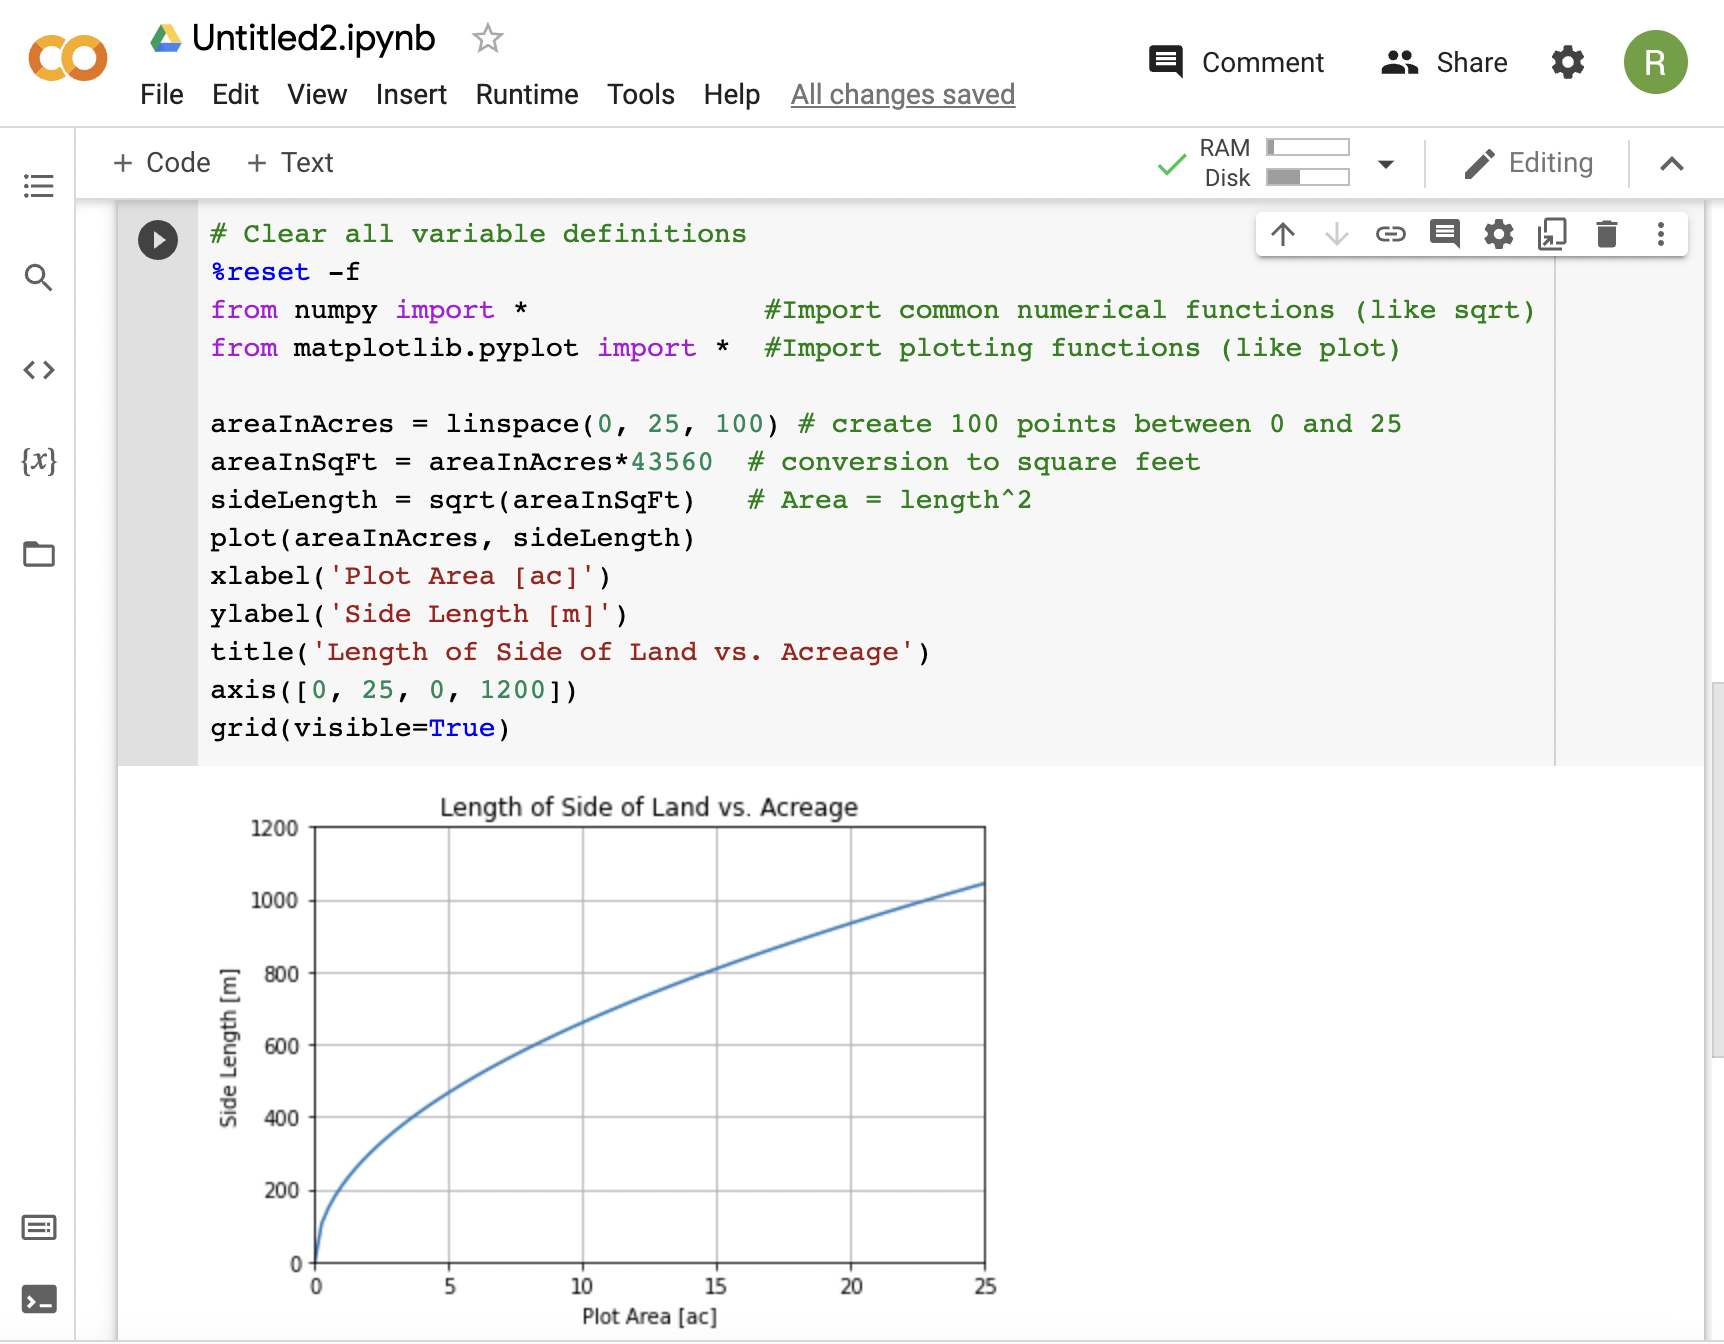
\includegraphics[width=0.9\textwidth]{ColabScreenshot3}
\caption{Google Colab, displaying a fully labeled plot.}
\label{fig:ColabScreenshot3}
\end{figure}

\begin{homework}
%--------------------------------------------------------------------
\question How are states, processes, and cycles related?
%--------------------------------------------------------------------
\question Describe the difference between an intensive and extensive property.
%--------------------------------------------------------------------
\question For each of the following properties, state whether it is intrinsic or extrinsic.
\begin{itemize}
\item Pressure
\item Volume
\item Kinetic energy
\item Specific internal energy
\end{itemize}
%--------------------------------------------------------------------
\question For each of the following systems, state whether it is open, closed, and/or isolated.
\begin{itemize}
\item The ice and water inside of a well-insulated cooler
\item An airtight piston, which is heated from the outside
\item A water spigot
\end{itemize}
%--------------------------------------------------------------------
\question Describe the difference between an isothermal process and an adiabatic process.

%--------------------------------------------------------------------
\question A soda can has a diameter of 2.13 inches and a height of 4.83 inches.  Additionally, it has a mass of 384 g.  Assuming the can is perfectly cylindrical, and the mass of aluminum is 14.7 g, determine:
\begin{itemize}
\item The volume of soda in the can (in ${\rm ft^3}$). \answer{[0.0100 ${\rm ft^3}$]}
\item The mass of soda in the can (in lbm). \answer{[0.812 lbm]}
\item The density of soda in the can (in $\frac{\rm kg}{\rm m^3}$) \answer{[1304 $\frac{\rm kg}{\rm m^3}$]}
\end{itemize}
%--------------------------------------------------------------------
\question The temperature in Chicago in winter can be as low as 14°F. What is the temperature in °C, K, and °R?
%--------------------------------------------------------------------
\question A piston with a diameter of 3'' compresses air, which is at an {\bf absolute} pressure of 2 atm.  What is the net force required to hold the piston still? Provide your answer in lbf. \answer{[103.9 lbf]}


Hint: don't forget atmosphere ($p_{atm}=1 \rm\ atm$) pushing on the other side.
%--------------------------------------------------------------------
\question Rework the previous question in Google Colab.  Plot the force required to hold the piston still, while varying the diameter of the piston between 1'' and 10''.  Plot your result, including a title and labels on both the x- and y- axes.
%--------------------------------------------------------------------
\question A barometer measures 690 mmHg.  What is the atmospheric pressure in kPa? \answer{[92 kPa]}
%--------------------------------------------------------------------
\question A manometer connects a tank with an unknown pressure to atmosphere.  If the manometer is filled with water at 20°C ($\rho = 1000 {\rm kg/m^3}$), and a height difference of 20 cm is measured, what is the gauge pressure in Pa?  \answer{[1962 Pa]}  If the atmospheric pressure is 101 kPa, what is the absolute pressure in Pa? \answer{[102.96 kPa]}
%--------------------------------------------------------------------
\end{homework}



\chapter{Properties of Matter} \label{ch:matter_properties}
In this chapter we consider the properties and relationships between properties of a pure substance (such as water) which can exist in three phases – solid, liquid and gas. We will not consider the solid phase in this course.

As you read through this chapter, you will notice that we always define a state through two properties.  Based on the state postulate, this is sufficient to fully define the state.  In other words, all properties of a state can be found, provided we know at least two.
\newpage
%--------------------------------------------------------------------
\section{Phase Change and Property Diagrams}
%--------------------------------------------------------------------
In order to introduce the rather complex phase change interactions that occur in pure substances we consider an experiment in which we have liquid water in a piston-cylinder device at 20°C and 100kPa pressure. Heat is added to the cylinder while the pressure is maintained constant until the temperature reaches 300°C, as shown the $T$-$v$ diagram (temperature vs. specific volume) in Figure \ref{fig:ch2_TvDiagram}.

\begin{figure}[H]
\centering
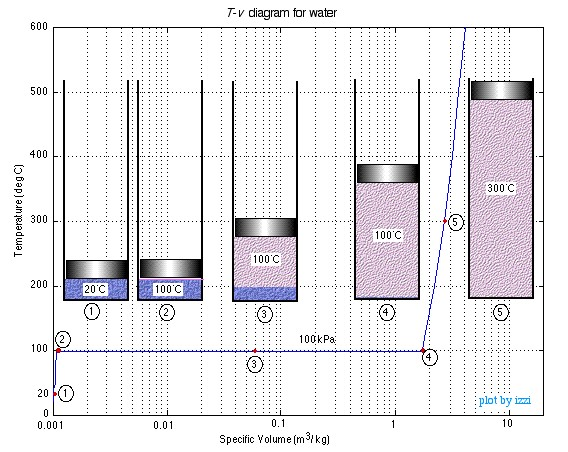
\includegraphics[width=0.9\textwidth]{TvDiagramForWater}
\caption{Heat is added to water at constant pressure, leading to boiling and an increase of volume.}
\label{fig:ch2_TvDiagram}
\end{figure}

From State (1) to State (2) the water maintains its liquid phase and the specific volume increases very slightly until the temperature reaches close to 100°C (State (2) – {\bf saturated liquid}). As more heat is added the water progressively changes phase from liquid to water vapor (steam) while maintaining the temperature at 100°C ({\bf saturation temperature} – $T_{sat}$) until there is no liquid remaining in the cylinder (State (4) – {\bf saturated vapor}). If heating continues then the water vapor temperature increases ($T > T_{sat}$) and is said to be {\bf superheated} (State (5)).

Notice that during this entire process the specific volume of the water increased by more than three orders of magnitude, which made it necessary to use a logarithmic scale for the specific volume axis.

This first experiment was performed at constant pressure.  If we increased the force on the piston (perhaps by increasing the mass of the piston), we could increase the pressure in the system.  Then, we could cool the system until it was a liquid, and repeat the experiment again. Figure \ref{fig:ch2_TvDiagram2} contains data from four such experiments, at 100 kPa, 1 MPa, 10 MPa, and 22 MPa.

\begin{figure}[H]
\centering
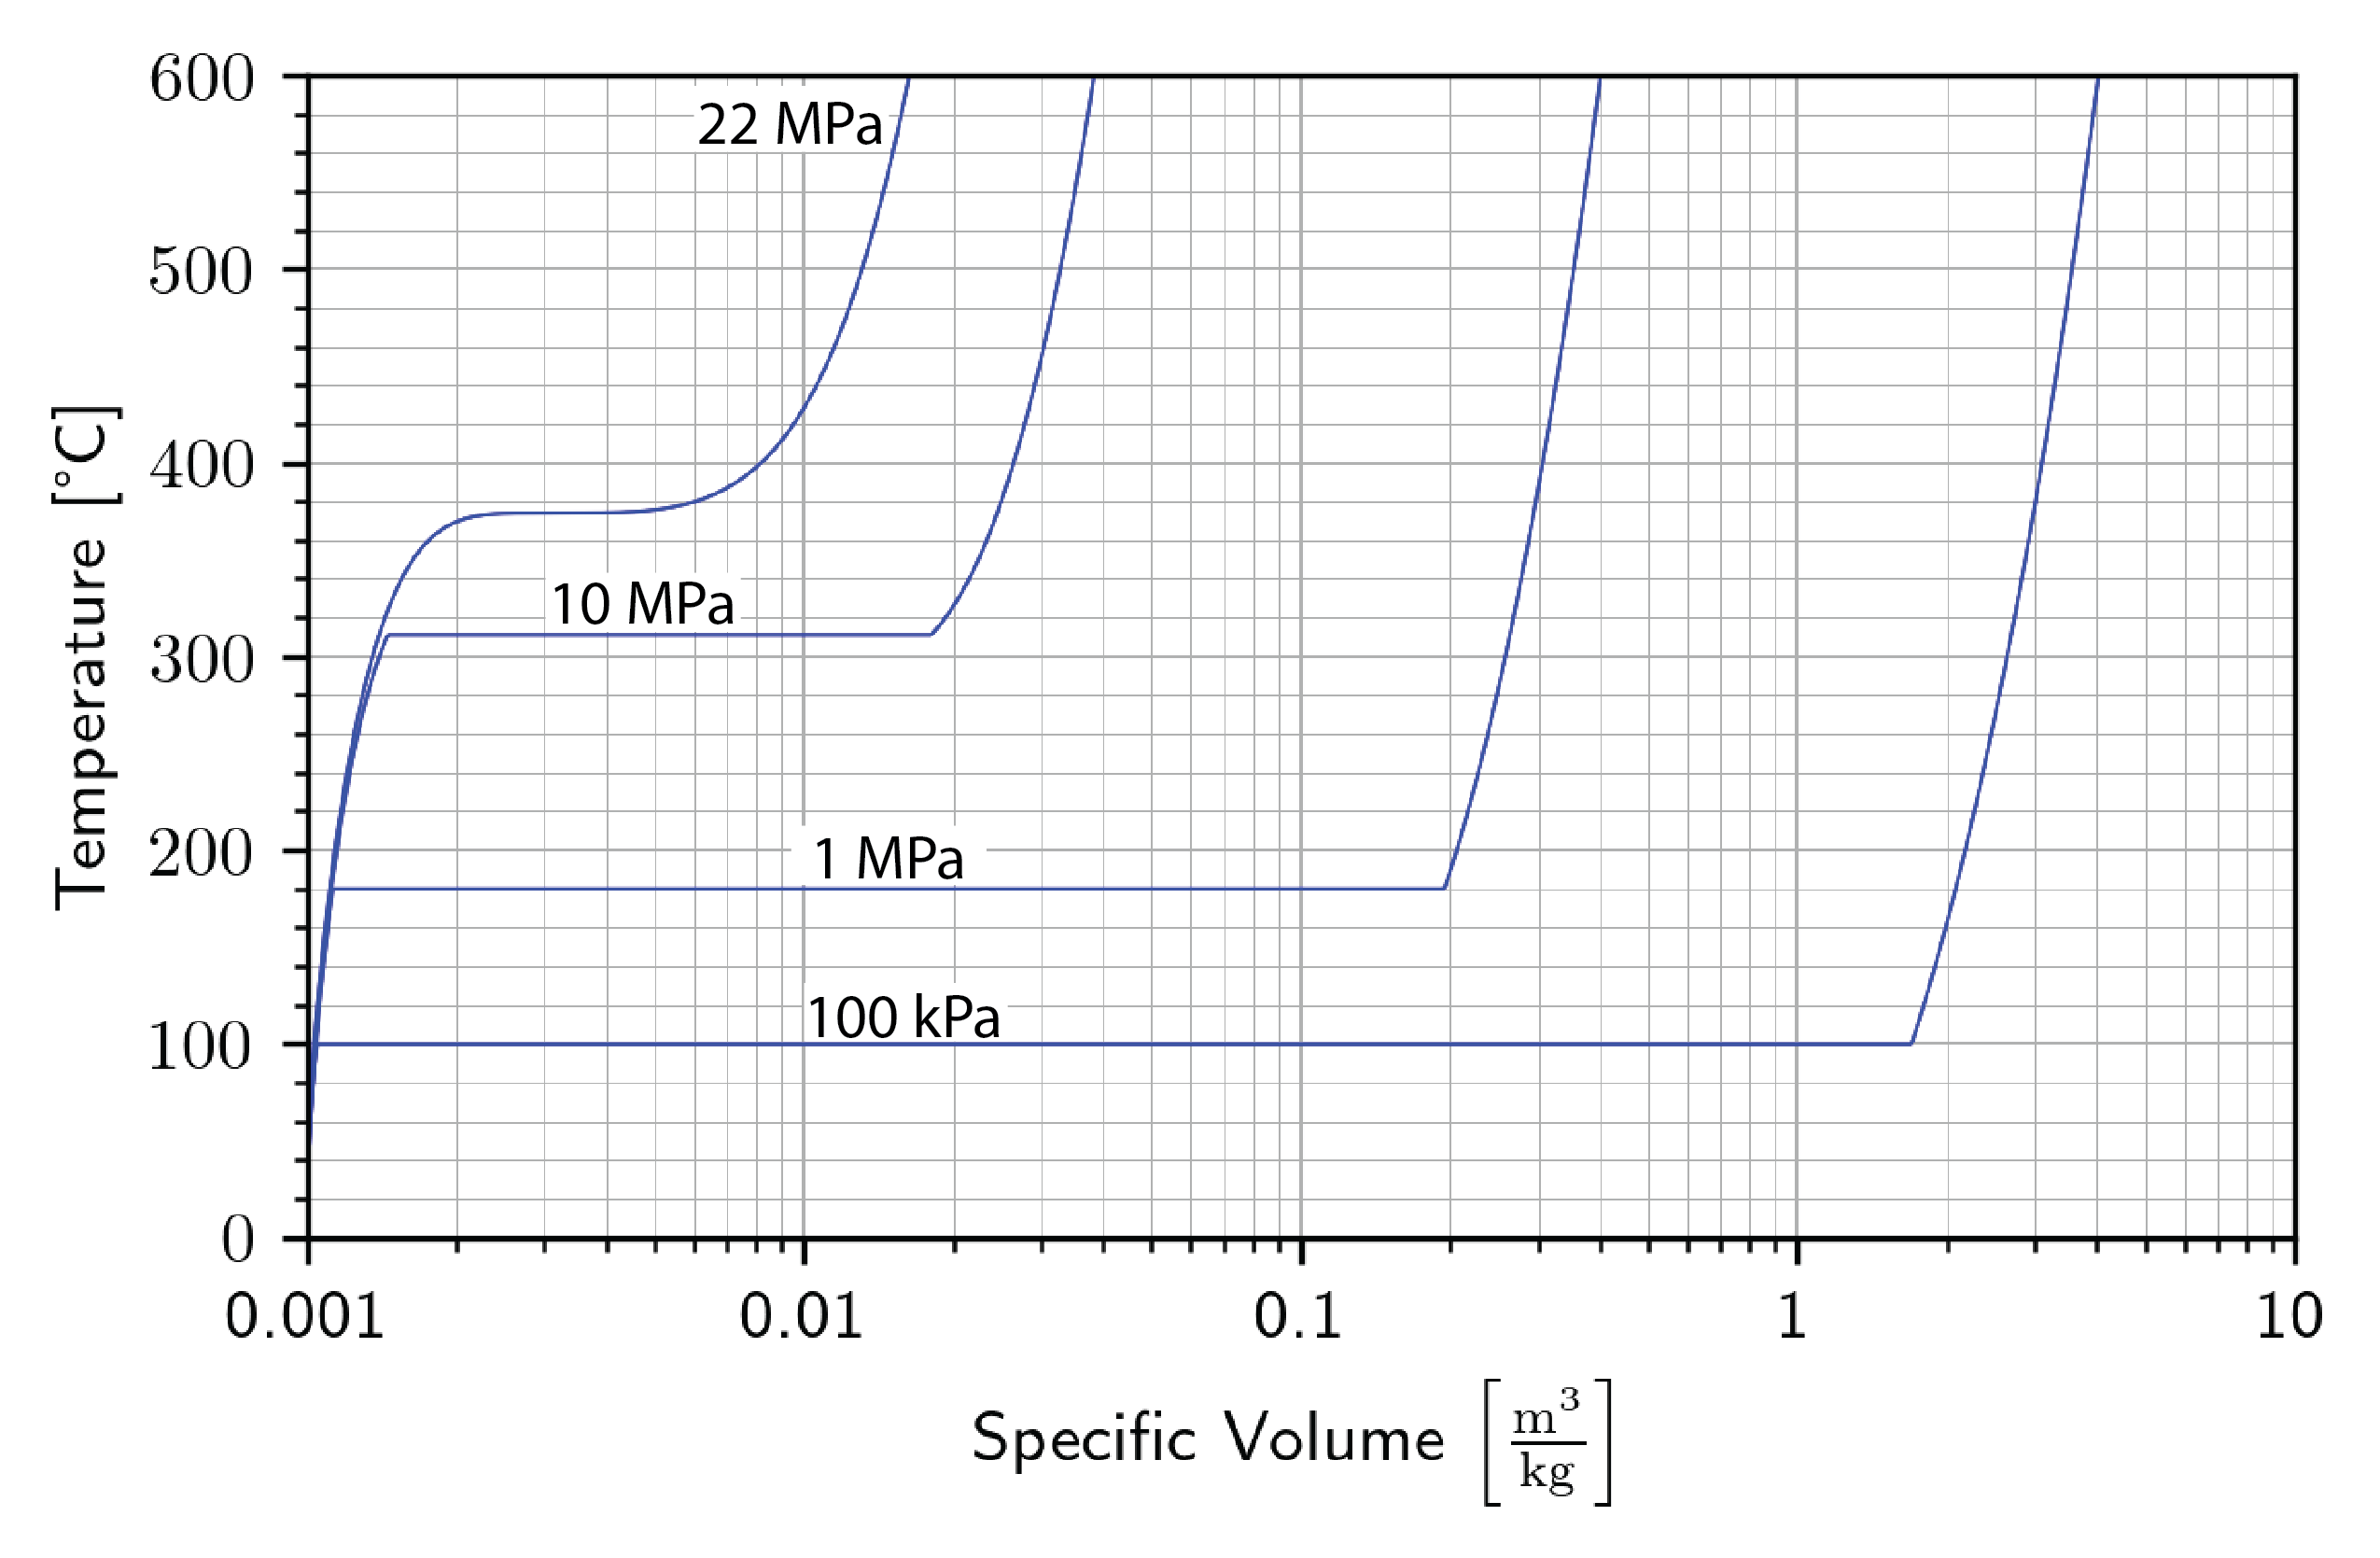
\includegraphics[width=0.9\textwidth]{isobars}
\caption{Heat is added to water at multiple pressures.}
\label{fig:ch2_TvDiagram2}
\end{figure}

As the pressure increases, the constant temperature region between saturated liquid and saturated vapor becomes smaller and smaller until it is eliminated completely at the critical point.  Above the critical point, there is no clear distinction between the liquid and vapor states.

Fluids with temperatures above the {\bf critical temperature} are known as {\bf supercritical fluids} or {\bf superheated} fluids.  Increasing the pressure will cause the fluid to be more liquid-like, and decreasing the pressure will cause the fluid to be more gas-like. 

To help distinguish between the regions of the $T$-$v$ diagram, we separate the liquid, vapor, and liquid-vapor mixtures with {\bf saturation lines}.  These lines are drawn by noting each saturated liquid and saturated vapor points, and connecting them.  The end result is shown in Figure \ref{fig:ch2_TvDiagram3}.

\begin{figure}[H]
\centering
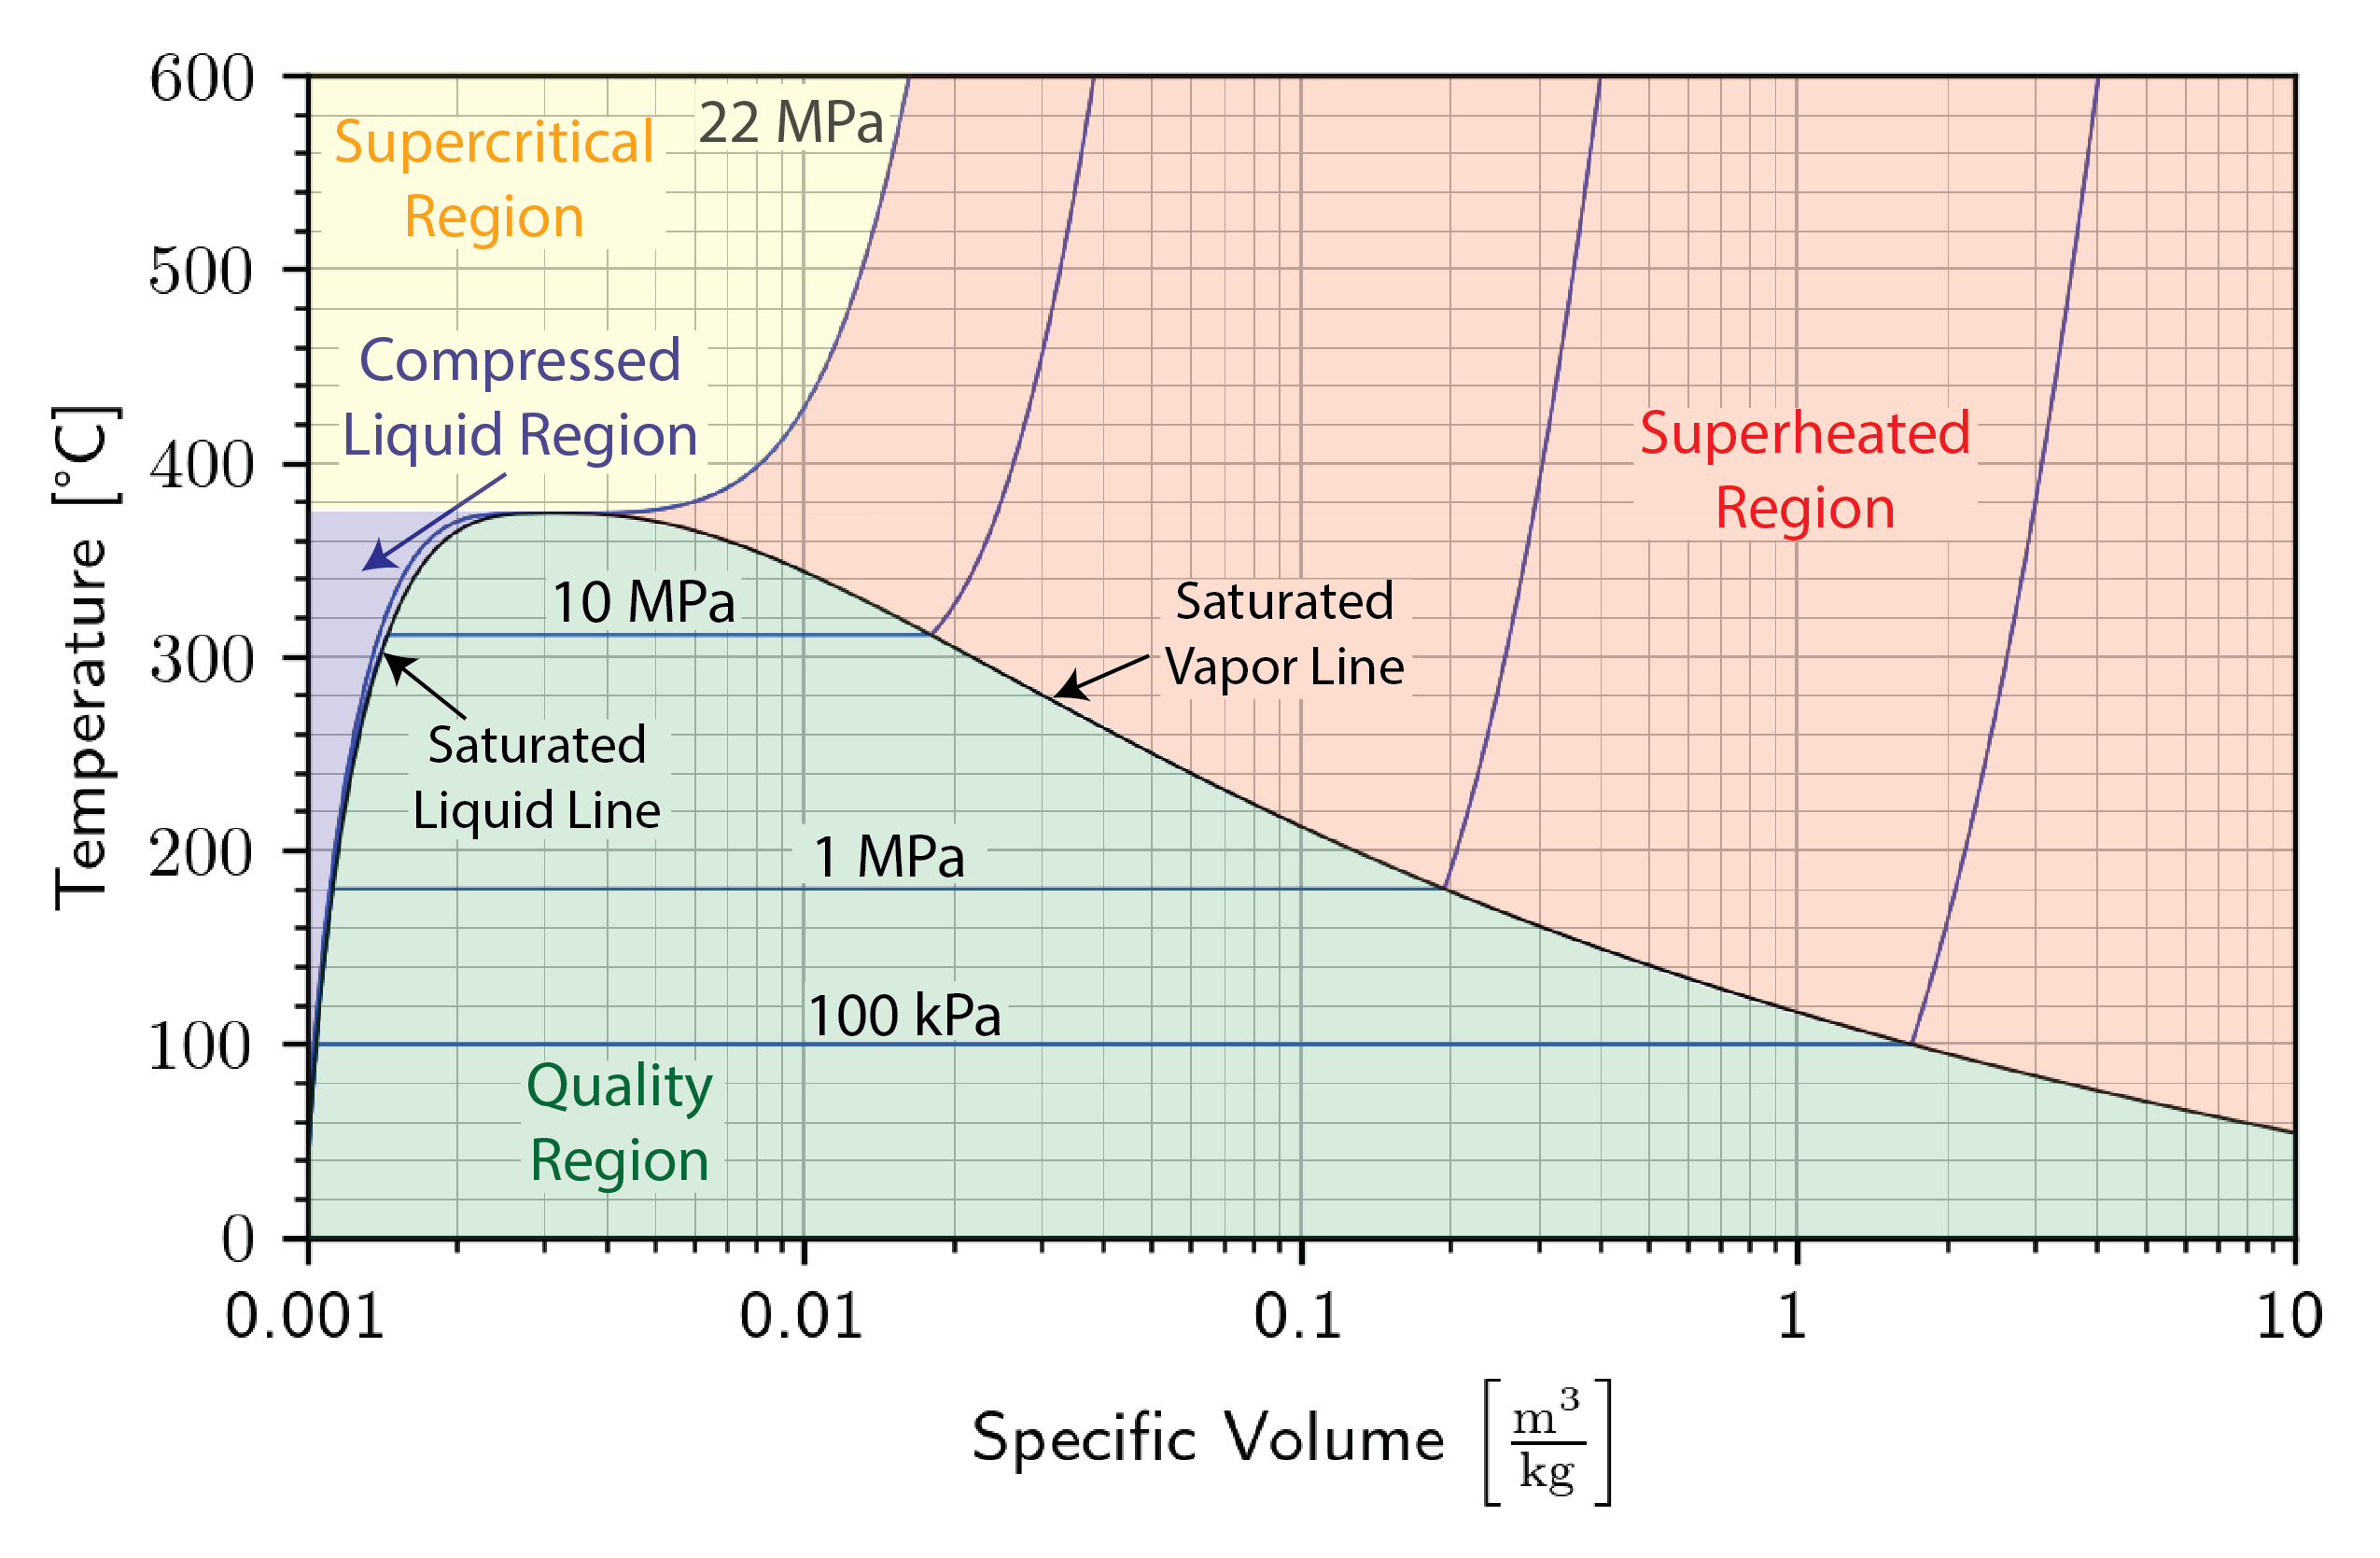
\includegraphics[width=0.9\textwidth]{TvDiagramWisobars}
\caption{$T$-$v$ diagram with saturation curves shown.}
\label{fig:ch2_TvDiagram3}
\end{figure}

The saturation lines define the regions of interest as shown in the diagram, being the {\bf compressed liquid} region to the left (blue), the {\bf quality} region or {\bf saturated} region enclosed by the saturation lines (green), and the {\bf superheated} region to the right of the saturated vapor line and critical pressure line (red), and the {\bf supercritical} region at temperatures and pressures higher than the critical point (yellow).

We will use {\bf property tables} associated with the regions in order to evaluate the various properties. Notice that we have provided property tables of steam and Refrigerant R134a in Appendix \ref{ch:appendixSteam} and \ref{ch:appendixR134a}.

\section{Quality}

The {\bf quality region}, also referred to as the {\bf saturated liquid-vapor mixture region}, is the area enclosed between the saturated liquid line and the saturated vapor line. At any point within this region the quality of the mixture (represented by the symbol $x$) is defined as the mass of vapor divided by the total mass of the fluid, as defined in Equation \ref{eq:quality}.
\begin{equation} \label{eq:quality}
  x = \frac{m_{\rm gas}}{m_{\rm total}}
\end{equation}

We can also use the {\bf rule of mixtures} to define mass-specific properties.  As an example, this is done for specific volume as follows:
\begin{align*}
  V &= V_f + V_g \\
  m v &= m_f v_f + m_g v_g \\
  m v &= (m-m_g) v_f + m_g v_g \\
  v &= \left(1 - \frac{m_g}{m}\right) v_f + \frac{m_g}{m} v_g \\
  v &= (1-x) v_f + x v_g
\end{align*}

Notice that properties relating to the saturated liquid have the subscript $f$, and those relating to the saturated vapor have the subscript $g$. If we consider a volume $V$ containing a mass $m$ of a saturated liquid-vapor mixture, we can calculate the quality $x$ as follows:

\begin{align}
  \nonumber v &= (1-x) v_f + x v_g\\
  \nonumber v &= v_f + x\left(v_g - v_f\right)\\
  \label{eq:quality2} x &= \frac{v - v_f}{v_g - v_f}
\end{align}

This is demonstrated graphically in Figure \ref{fig:ch2_TvDiagram4}.

\begin{figure}[H]
\centering
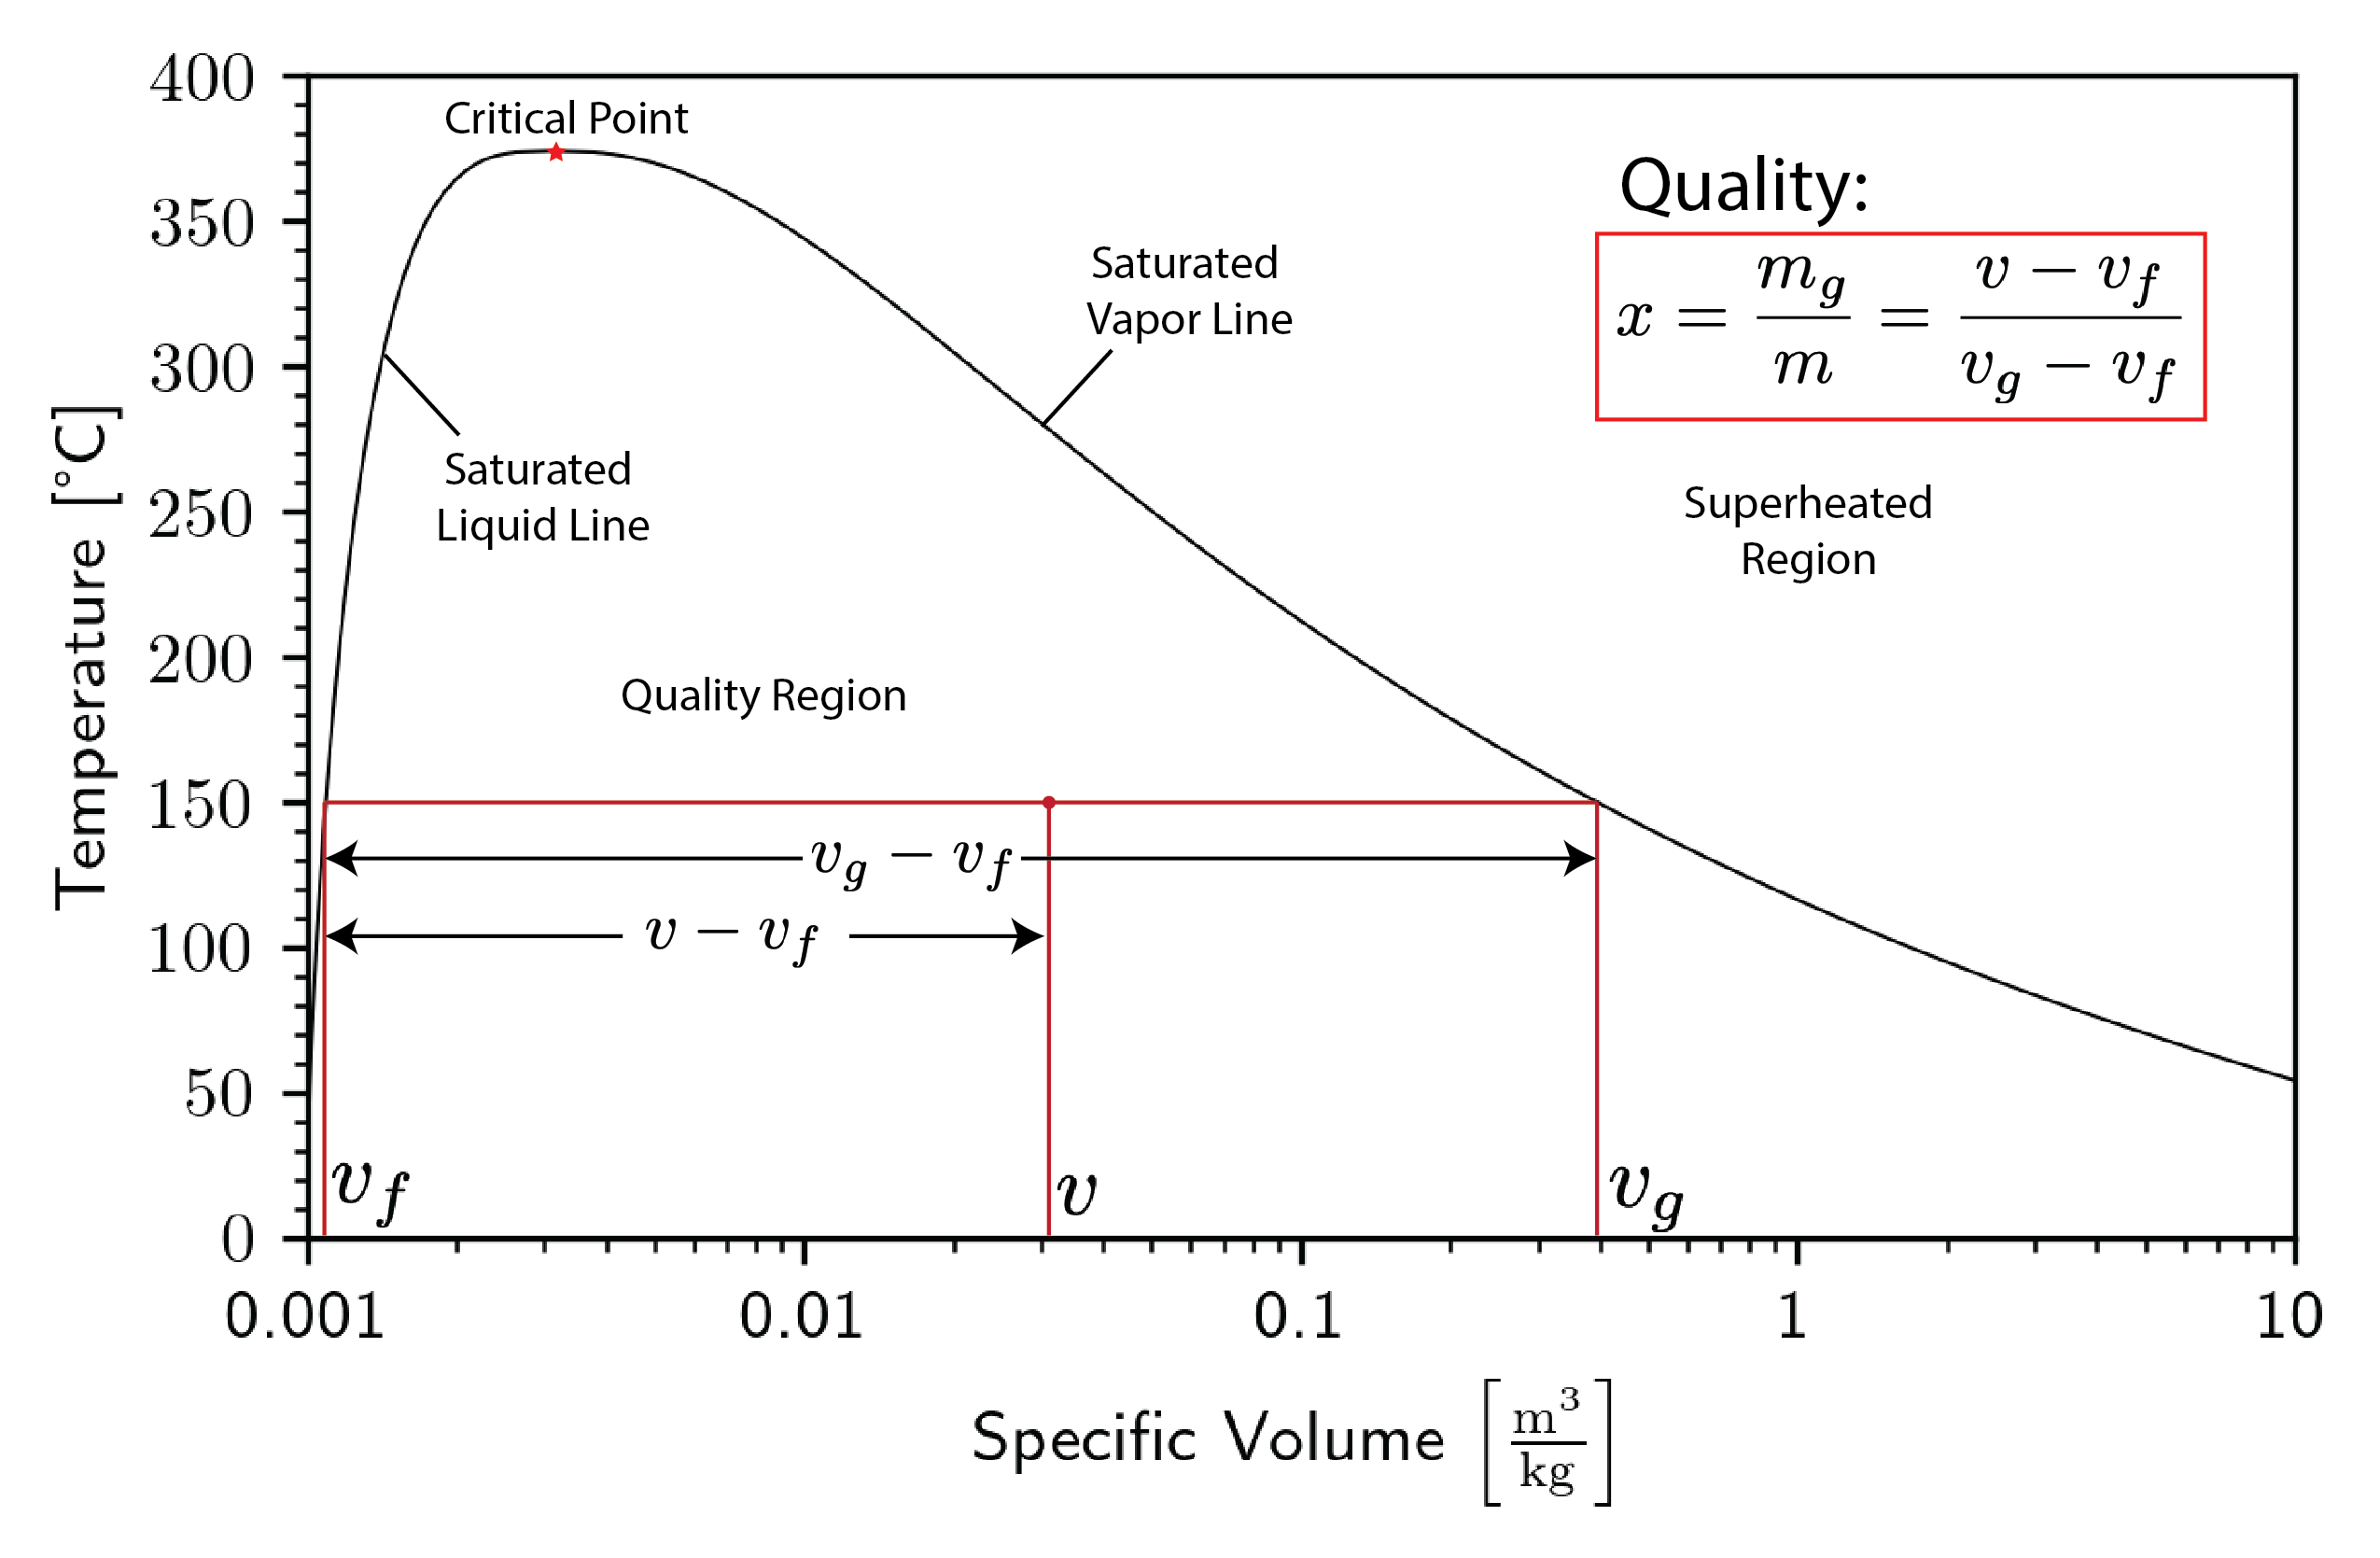
\includegraphics[width=1.0\textwidth]{TvDiagramQuality}
\caption{Quality is the ratio of the mass of gas to the total mass within the system.}
\label{fig:ch2_TvDiagram4}
\end{figure}

%% \begin{figure}[H]
%% \centering
%% 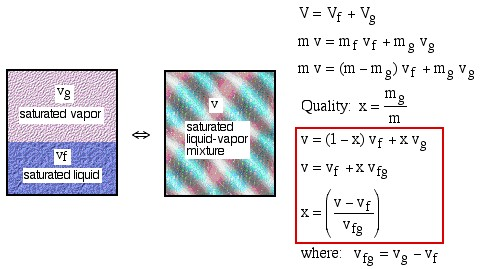
\includegraphics[width=0.75\textwidth]{VolumeEquations}
%% \caption{Quality can also be defined based on the specific volumes of the liquid ($v_f$) and gas ($v_g$).}
%% \label{fig:ch2_VolumeEquations}
%% \end{figure}

Typically, because of the extremely large range of specific volume values of interest, the $T$-$v$ diagram can only be done on a semi-log plot (logarithmic scaling on the $x$-axis). This is extremely inconvenient, so instead the $T$-$v$ diagram is normally not drawn to scale. Instead, it is only sketched in order to help define the problem, which is then solved in terms of the steam tables. This approach is illustrated in an example below.

\begin{example}{Boiling Water}
  Two kilograms of water at 25°C are placed in a piston cylinder device under 100 kPa pressure (state (1)). Heat is added to the water at constant pressure until the piston reaches the stops at a total volume of 0.4 m3 (state (2)). More heat is then added at constant volume until the temperature of the water reaches 300°C (state (3)). Determine (a) the quality of the fluid and the mass of the vapor at state (2), and (b) the pressure of the fluid at state (3).


{\bf Step 1: Diagram} \quad  \underline{Always} draw a complete diagram of the states and processes of the problem and include all the relevant information on the diagram. In this case there are three states and two processes (constant pressure and constant volume).

\begin{center}
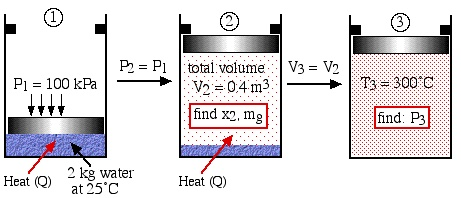
\includegraphics[width=0.75\textwidth]{example2-1}
%\captionof{figure}{}
%\label{fig:ch2_example1}
\end{center}

{\bf Step 2: $p$-$v$ or $T$-$v$} \quad  In the case of a closed system with a phase change fluid, always sketch a $T$-$v$ or $p$-$v$ diagram indicating all the relevant states and processes on the diagram. As mentioned above this diagram will not be drawn to scale, however it will help to define the problem and the approach to solution. In the case of steam, as we determine various values from the steam tables we add these values to the diagram, typically as shown below:

\begin{center}
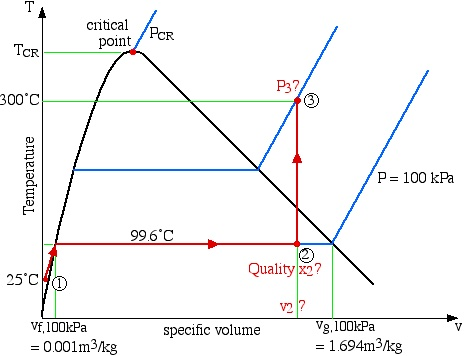
\includegraphics[width=0.6\textwidth]{example2-1_Tv}
%\captionof{figure}{}
%\label{fig:ch2_example1_Tv}
\end{center}


{\bf Step 3: Address Prompt} \quad Notice that the $T$-$v$ diagram is based exclusively on intensive properties, hence mass is not indicated on the diagram. Thus we indicate on the diagram that in order to determine the quality at state (2) we need to first evaluate the specific volume $v_2$, which can then be compared to the saturation values $v_f$ and $v_g$ at the pressure of 100 kPa.

Thus:
\begin{equation*}
  v_2 = \frac{V}{m} = \frac{0.4\ \rm m^3}{\rm 2\ kg} = 0.2 \frac{\rm m^3}{kg}
\end{equation*}

Quality can be found via Equation \ref{eq:quality2}:

\begin{equation*}
  x_2 = \frac{v_2-v_f}{v_g-v_f} = \frac{0.2 - 0.001}{1.694-0.001}\rightarrow \redbox{x_2 = 0.118}
\end{equation*}

Finally, the mass of water vapor:
\begin{equation*}
  x = \frac{m_g}{m_{tot}} \rightarrow m_{g_2} = x_2\cdot m_{tot} = 0.118 \cdot 2\ {\rm kg} \rightarrow \redbox{m_{g_2} = 0.235\ {\rm kg}}
\end{equation*}

Concerning state (3), the problem statement did not specify that it is in the superheated region. We needed to first determine the saturated vapor specific volume $v_g$ at 300°C. This value is 0.0216 $\rm m^3$/kg, which is much less than the specific volume $v_3$ of 0.2 $\rm m^3$/kg, thus placing state (3) well into the superheated region. Thus the two intensive properties which we use to determine the pressure at state (3) are $T_3$=300°C, and $v_3$=0.2 $\rm m^3$ / kg. On scanning the superheated tables we find that the closest values lie somewhere between 1.2 MPa and 1.4 MPa, thus we use linear interpolation techniques to determine the actual pressure $p_3$ as shown below:

\begin{center}
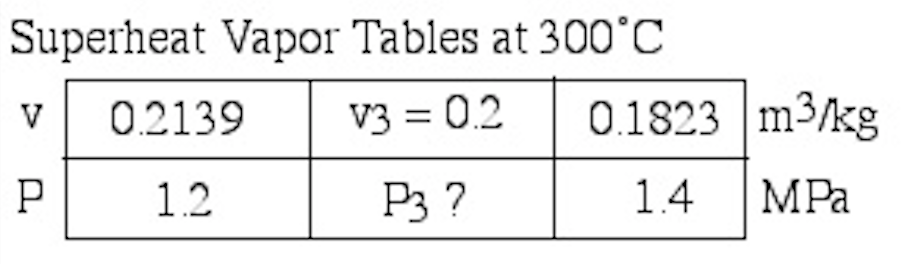
\includegraphics[width=0.5\textwidth]{example2-1_p3}
%\captionof{figure}{}
%\label{fig:ch2_example1_p3}
\end{center}

Linear interpolation has a good description from \href{https://en.wikipedia.org/wiki/Linear_interpolation}{Wikipedia}, but we will use it as follows:
\begin{equation*}
  \frac{\Delta p_A}{\Delta p_b} = \frac{\Delta v_A}{\Delta v_b} \rightarrow \frac{p_3 - 1.2}{1.4-1.2} = \frac{0.2-0.2139}{0.1823-0.2139} = 0.440
\end{equation*}

Therefore, $\redbox{p_3=1.29\ \rm MPa.}$

\end{example}

If you check the steam property tables, you will see that we have also included three new properties: internal energy $u$ [kJ/kg], enthalpy $h$ [kJ/kg], and entropy $s$ [kJ/kgK].  All of these will be defined as needed in future sections. At this stage we note that the 3 equations relating quality and specific volume can also be evaluated in terms of these three additional properties.

\begin{align*}
  u &= (1-x)\ u_f + x\ u_g \\
  h &= (1-x)\ h_f + x\ h_g \\
  s &= (1-x)\ s_f + x\ s_g
\end{align*}

% --------------------------------------------------------------------
\section{The $p$-$v$ Diagram for Water}
% --------------------------------------------------------------------
The above discussion was done in terms of the temperature ($T$) and specific volume ($v$). You may recall from Chapter 1 when we defined the State Postulate however, that any two independent intensive properties can be used to completely define all other intensive state properties. This means we can also evaluate a substance in terms of pressure ($p$) and specific volume ($v$) as shown below:

\begin{figure}[H]
\centering
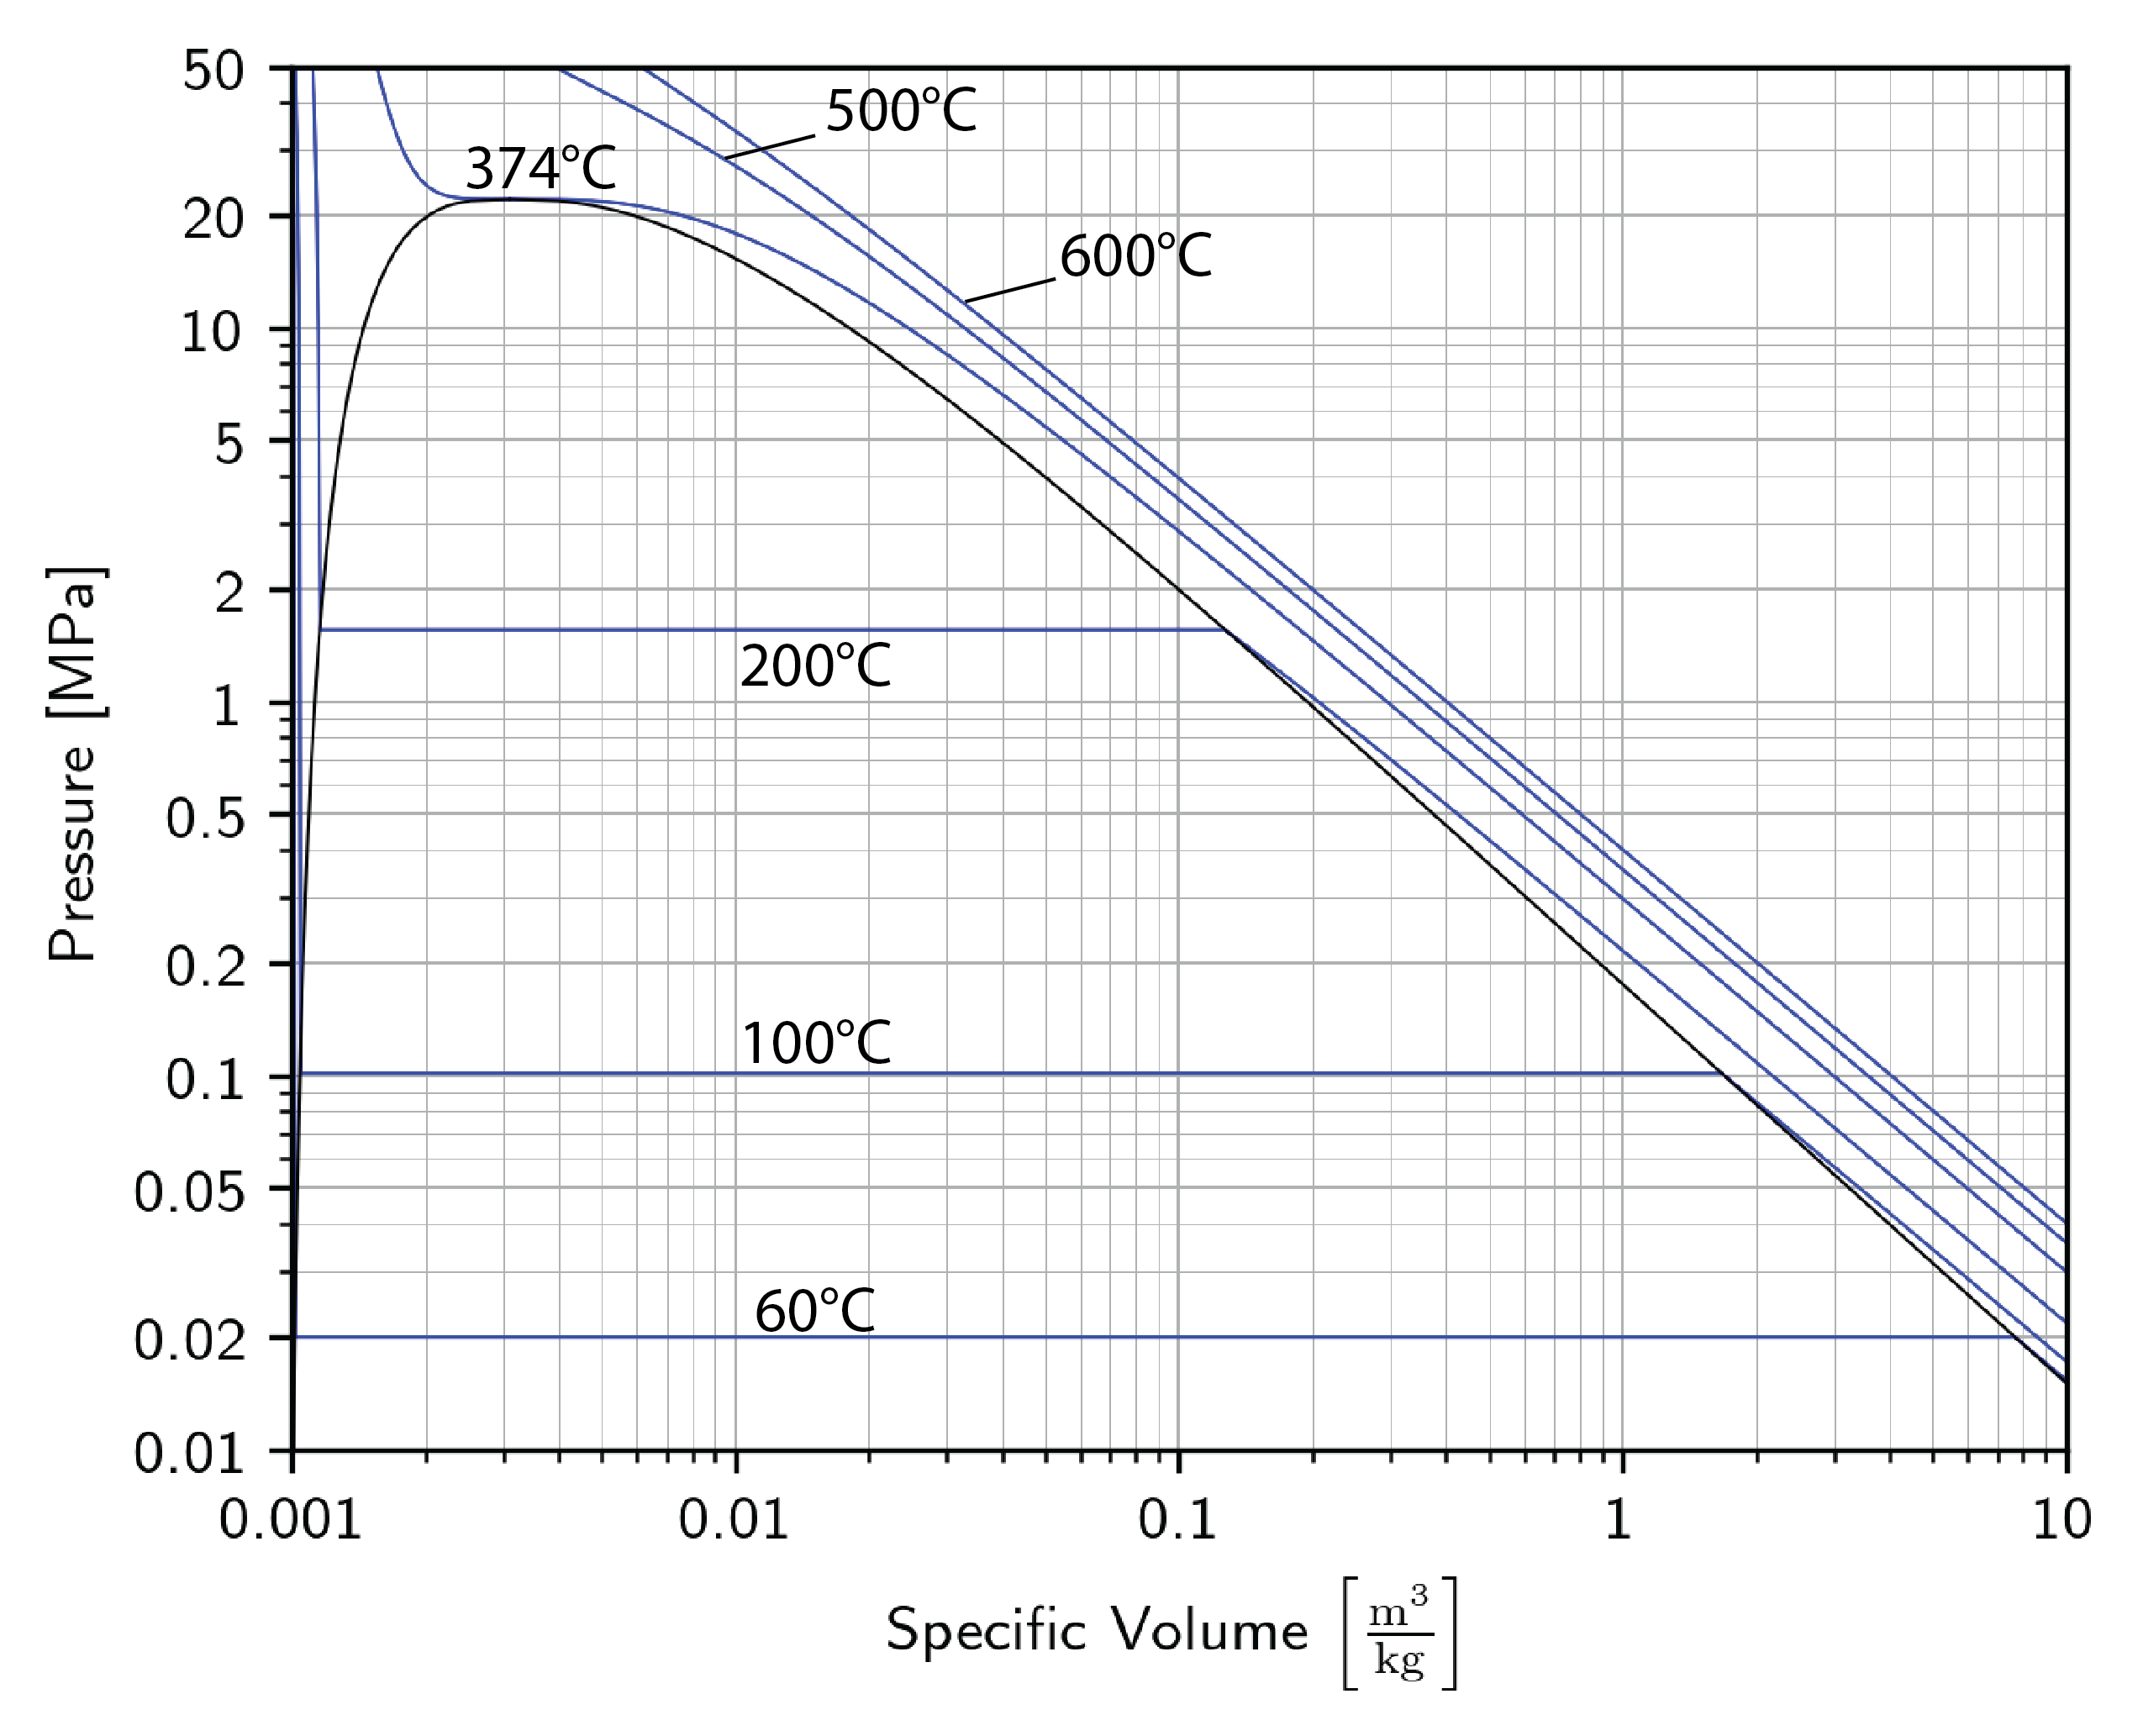
\includegraphics[width=0.75\textwidth]{pvDiagramWisothermal}
\caption{Variation of pressure and specific volume for water at various temperatures.  Note that both the x- and y- axes are logarithmic.}
\label{fig:ch2_PvDiagram}
\end{figure}

Similar to the $T$-$v$ diagram, we typically only sketch the $p$-$v$ diagram to solve problems, as seeing all relevant data requires a log-log plot.  Again, the example below illustrates this process.

\begin{example}[label={ex:ch2constantPressure}]{Constant Pressure Expansion}
  Two kilograms of water at 25°C are placed in a piston cylinder device under 3.2 MPa pressure as shown in the diagram (State (1)). Heat is added to the water at constant pressure until the temperature of the fluid reaches 350°C (State (2)). Determine the final volume of the fluid at state (2).

  {\bf Step 1: Diagram} \quad In this case, there are only two states.

\begin{center}
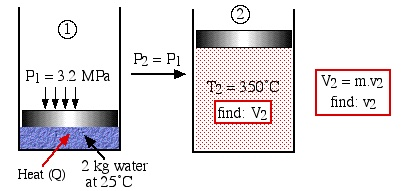
\includegraphics[width=0.6\textwidth]{example2-2_diagram}
%\captionof{figure}{State diagram for Example 2.2}
%\label{fig:ch2_example2_diagram}
\end{center}  

{\bf Step 2: $p$-$v$ or $T$-$v$} \quad In this example since the pressure is known (3.2 MPa) and remains constant throughout the process, we find it convenient to draw a $p$-$v$ diagram indicating the process (1) - (2) as follows.

\begin{center}
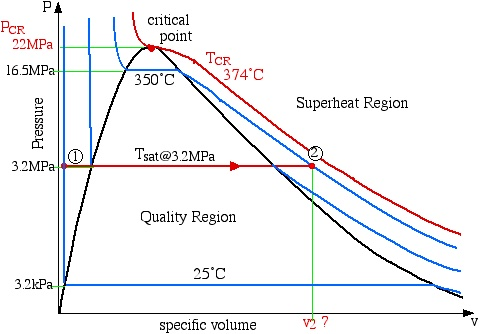
\includegraphics[width=0.75\textwidth]{example2-2_pv}
%\captionof{figure}{State diagram for Example 2.2}
%\label{fig:ch2_example2_diagram}
\end{center}

{\bf Step 3: Address Prompt} \quad As in the previous example, on scanning the superheated tables we find that we need to interpolate between pressure $p$=3.0 MPa and $p$=3.5 MPa in order to determine the specific volume at the required pressure of 3.2 MPa as follows:

\begin{center}
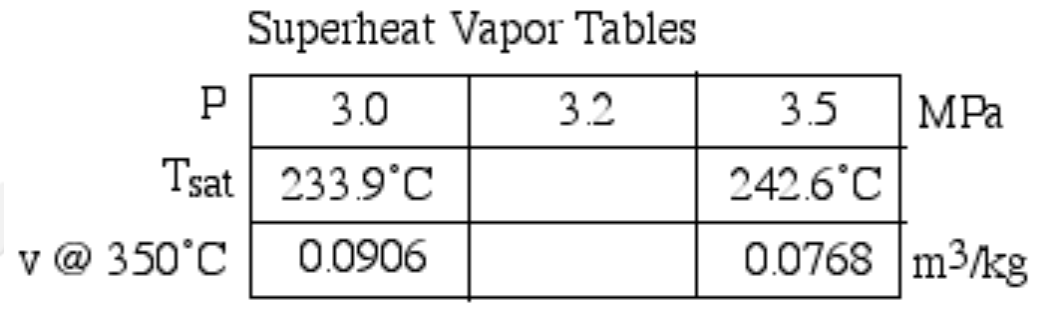
\includegraphics[width=0.6\textwidth]{example2-2_tables}
%\captionof{figure}{State diagram for Example 2.2}
%\label{fig:ch2_example2_diagram}
\end{center}

\begin{equation*}
  \frac{\Delta p_A}{\Delta p_b} = \frac{\Delta v_A}{\Delta v_b} \rightarrow \frac{3.2 - 3.0}{3.5-3.0} = \frac{v_2-0.0906}{0.0768-0.0906} = 0.4
\end{equation*}
Therefore, $v_2 = 0.085 \frac{\rm m^3}{\rm kg}$ and \redbox{V_2 = 0.17\ \rm m^3.}

\end{example}

% --------------------------------------------------------------------
\section{Ideal Gas Equation of State}
% --------------------------------------------------------------------
We find that for a pure substance in the superheated region, at specific volumes much higher than that at the critical point, the $p$-$v$-$T$ relation can be conveniently expressed by the {\bf ideal gas equation of state} to a high degree of accuracy, as follows:
\begin{equation} \label{idealGasLaw}
  p v = R T
\end{equation}
where: $R$ is constant for a particular substance and is called the {\bf gas constant}.

Note that for the ideal gas equation both the pressure $p$ and the temperature $T$ must be expressed in absolute quantities.

The gas constant R can be expressed as follows:

\begin{equation}
  R = \frac{R_u}{M} \left[\frac{\rm kJ}{\rm kg \cdot K}\right]
\end{equation}

where $R_u = 8.314 \frac{\rm kJ}{\rm kmol \cdot K}$, and is known is the {\bf universal gas constant}.  $M$ is the molar mass of the gas, measured in $\left[\frac{\rm kg}{\rm kmol}\right]$ or $\left[\frac{\rm lbm}{\rm lbmol}\right]$ (which yield the same numerical value).
For air,
\begin{equation*}
  M = 28.97 \frac{\rm kg}{\rm kmol} \rightarrow R_{air} = 0.287 \frac{\rm kJ}{\rm kg\cdot K}
\end{equation*}

For water/steam,
\begin{equation*}
  M = 18.02 \frac{\rm kg}{\rm kmol} \rightarrow R_{H_2O} = 0.4615 \frac{\rm kJ}{\rm kg\cdot K}
\end{equation*}

\begin{example}{Checking the Ideal Gas Law}
A piston-cylinder device contains 0.5 kg saturated liquid water at a pressure of 200 kPa. Heat is added and the steam expands at constant pressure until it reaches 300°C.

a) Draw a diagram representing the process showing the initial and final states of the system.

b) Sketch this process on a T-v (temperature-specific volume) diagram with respect to the saturation lines, critical point, and relevant constant pressure lines, clearly indicating the initial and final states.

c) Using steam tables determine the initial temperature of the steam prior to heating.

d) Using steam tables determine the final volume of the steam after heating

e) Using the ideal gas equation of state determine the final volume of the steam after heating. Determine the percentage error of using this method compared to that of using the steam tables.


{\bf Solution:}

Even if questions a) and b) were not required, this should always be the first priority item in solving a thermodynamic problem.

\begin{center}
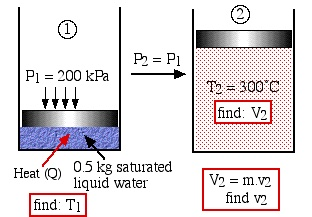
\includegraphics[width=0.5\textwidth]{example2-5_diagram}
%\captionof{figure}{State diagram for Example 2.2}
%\label{fig:ch2_example2_diagram}
\end{center}

\begin{center}
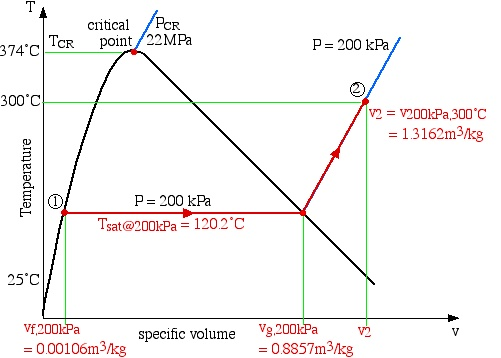
\includegraphics[width=0.5\textwidth]{example2-5_Tv}
%\captionof{figure}{State diagram for Example 2.2}
%\label{fig:ch2_example2_diagram}
\end{center}

c) Since state (1) is specified as saturated liquid at 200 kPa, we use the saturated pressure steam tables to determine that $\redbox{T_1=T_{sat}(200{\rm kPa}) = 120.2°{\rm C}}$.

d) From the $T$-$v$ diagram we determine that state (2) is in the superheated region, thus we use the superheated steam tables to determine that $v_2$ = $v({\rm 200kPa,300°C}$ = 1.3162 m3/kg. Thus $V_2 = m\cdot v_2 = (0.5{\rm kg})\cdot (1.3162 {\rm m^3/kg}) = \redbox{0.658 {\rm m^3}} = 658 {\rm L}$

e) We use $pv = RT$ as our base equation.  Note that pressure and temperature must be absolute!

\begin{equation*}
  v = \frac{RT}{p} \rightarrow v_2 = \frac{0.4615\ {\rm kJ/(kg\cdot K)} \cdot (300 + 273)\ {\rm K}}{200 \rm\ kPa} = 1.322 \frac{\rm m^3}{\rm kg}
\end{equation*}

Therefore, $V_2 = m\cdot v_2 = = (0.5{\rm kg})\cdot (1.322 {\rm m^3/kg}) = \redbox{0.661 {\rm m^3}} = 661 {\rm L}$.

Finally, we calculate error:
\begin{equation*}
  {\rm error} = \left|\frac{\rm true\ value - estimated\ value}{\rm true\ value}\right| = \left|\frac{0.658 - 0.661}{0.658}\right|\approx 0.005 = \redbox{0.5\%}
\end{equation*}

\end{example}

As a side-note, we see the unit ratio $\rm kJ / kPa$ quite often.  Expanding these out results in:
\begin{equation*}
  \frac{\rm kJ}{\rm kPa} = \frac{\rm kN\cdot m}{\rm kN / m^2} = {\rm m}^3
\end{equation*}

\section{Non-Ideal Gas Behavior}
The $T$-$v$ diagram for water is shown below, with the addition of error that arises from calculating the pressure through the ideal gas law.

\begin{figure}[H]
\centering
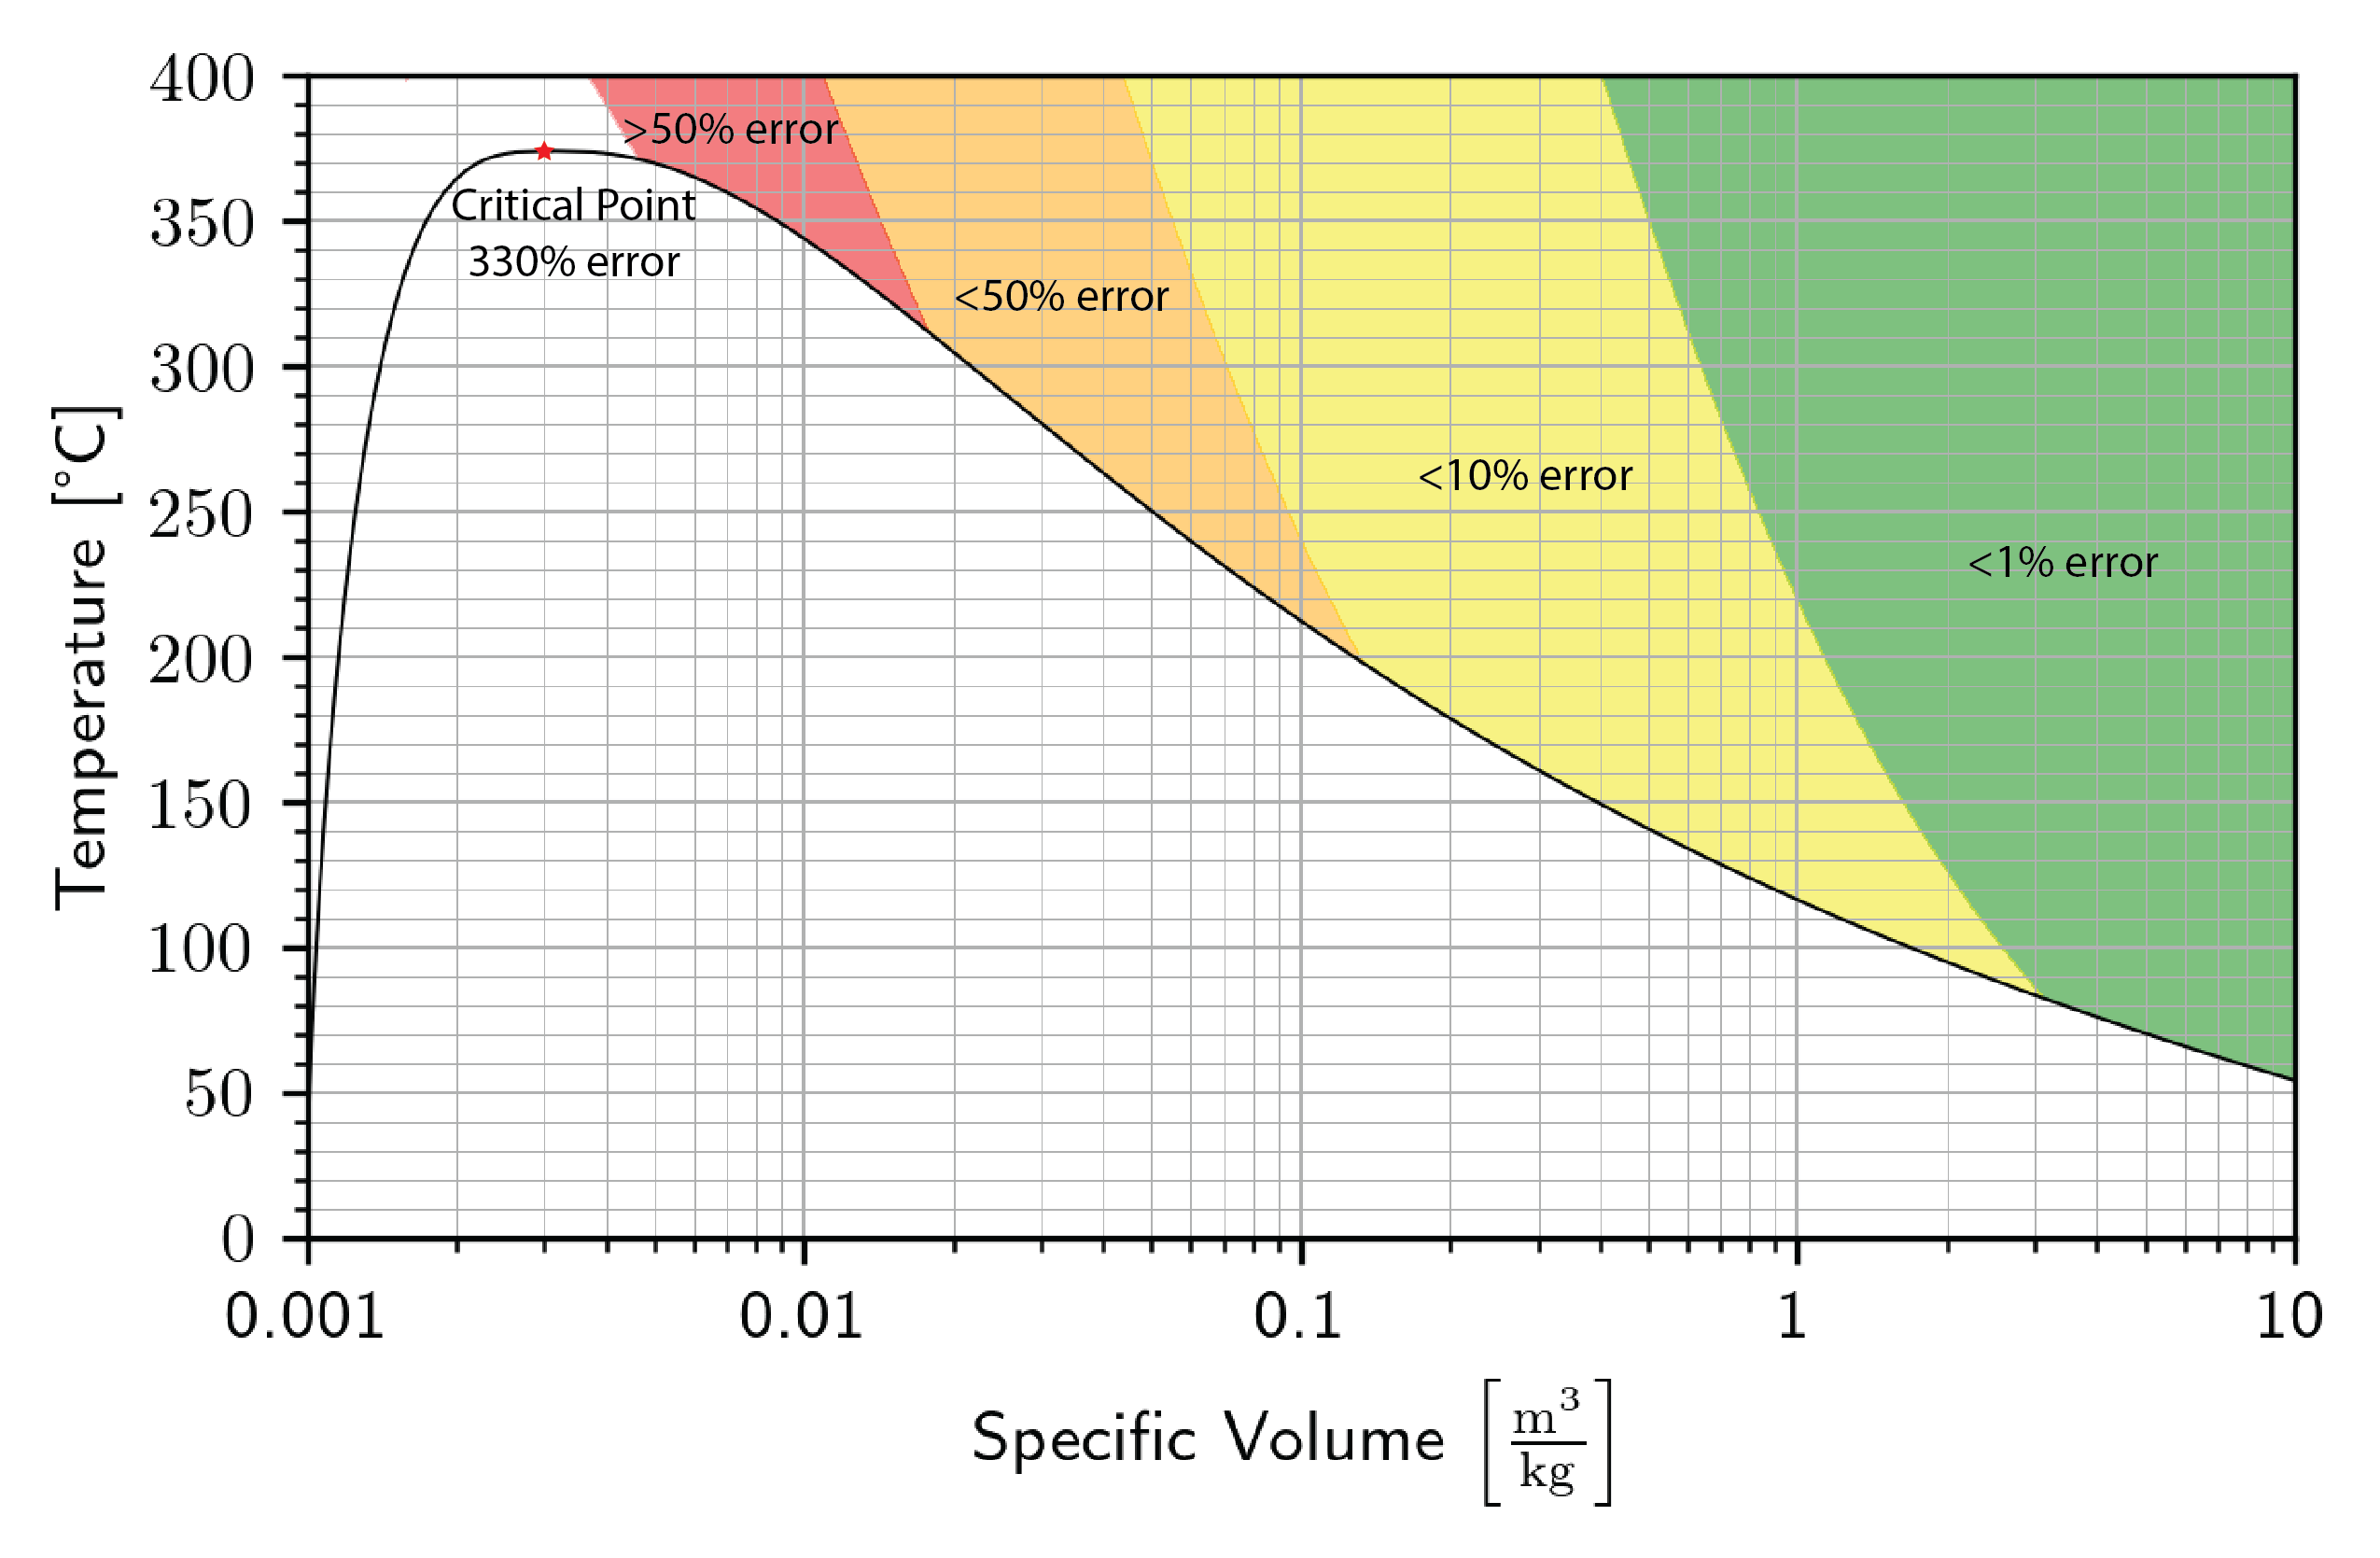
\includegraphics[width=1.0\textwidth]{IdealGasErrorTv}
\caption{$T$-$v$ diagram, including errors from ideal gas equation of state.}
\label{fig:ch2_Tv-ideal}
\end{figure}

Note that error tends to decrease somewhat as temperature increases, but is much more affected by specific volume (and therefore pressure). Note that at the critical point the error is 330\%.  This non-ideal behavior can be accounted for by a correction factor called the {\bf compressibility factor} $Z$ defined as follows:

\begin{equation}
  pv = ZRT \rightarrow Z = \frac{pv}{RT}
\end{equation}

When the compressibility factor Z approaches 1, the gas behaves as an ideal gas. By specifying both temperature and pressure, the compressibility factor can be expressed as:

\begin{equation} \label{eq:ch2_Zdef}
  Z = \frac{v_{actual}}{v_{ideal}}
\end{equation}

All fluids normalized in this manner exhibit similar non-ideal gas behavior within a few percent, thus they can all be plotted on a Generalized Compressibility Chart. A number of these charts are available, however we prefer to use the Lee-Kesler (logarithmic) Compressibility Chart, shown below.


\begin{figure}[H]
\centering
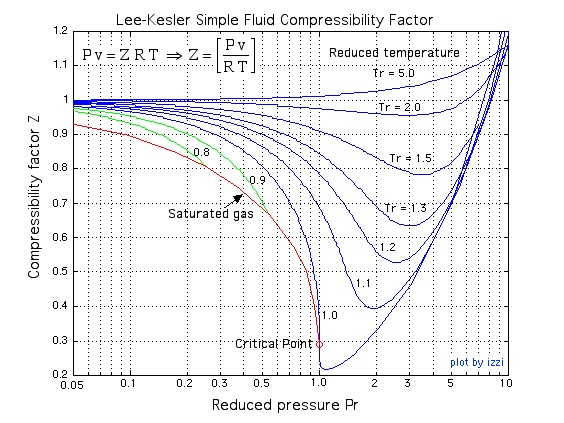
\includegraphics[width=0.75\textwidth]{Zfactor}
\caption{Compressibility factor for non-ideal gases.}
\label{fig:ch2_Zfactor}
\end{figure}

Notice that the compressibility factor is dependent on the reduced pressure and temperature.  These are defined as follows:
\begin{align}
  p_R &= \frac{p}{p_{crit}} &   T_R &= \frac{T}{T_{crit}}
\end{align}

Different fluids have different values of critical point pressure and temperature data $p_{crit}$ and $T_{crit}$, and these can be determined from the Table of Critical Point Data of Various Substances in Appendix \ref{sec:idealGasProps}.

\begin{example}[label={ex:ch2idealGas}]{Correcting the Ideal Gas Law}
  Carbon Dioxide gas is stored in a 100 liter tank at 6 MPa and 30°C. Determine the mass of $\rm CO_2$ in the tank based on (a) the ideal gas equation of state, (b) the generalized compressibility chart, and (c) values obtained from the $\rm CO_2$ tables of data.  Determine the percentage error in each case.

  {\bf Solution Approach:}

  There is only one state here, so there is little to gain by drawing the state diagrams.  Likewise, the $T-v$ diagram is useful when using tables, but we want to use the ideal gas law for our calculations.

  For $\rm CO_2$, the molar mass is $M = 44.01 \frac{\rm kg}{\rm kmol}$, which leads to a gas constant of $R_{CO_2}=0.1889 \frac{\rm kJ}{\rm kg\cdot K}$.  We can use this in the ideal gas equation of state:

  \begin{equation*}
    v_{ideal} = \frac{R\cdot T}{p} = \frac{0.1889 \frac{\rm kJ}{\rm kg\cdot K} \cdot 303\ {\rm K}}{6000\ {\rm kPa}}= 0.00954 \frac{\rm m^3}{\rm kg}
  \end{equation*}

  Mass can then be found from the equation $V = m \cdot v$:
  \begin{equation*}
    m_{ideal} = \frac{V}{v} = \frac{100\ \rm L}{0.00954 \frac{\rm m^3}{\rm kg}} \cdot \frac{1\ \rm m^3}{1000\ \rm L} \rightarrow \redbox{m_{ideal} = 10.5\ {\rm kg}}
  \end{equation*}
  
  To use the compressibility chart, we need to find the critical temperature and pressure for $\rm CO_2$.  This comes from the Table of Critical Point Data of Various Substances (Appendix \ref{sec:idealGasProps}): $p_{crit} = 7.39\ {\rm MPa}$, $T_{crit} = 304.2\ K$.

  Next, we calculate our reduced temperature and pressure:
  \begin{align*}
    p_R = \frac{p}{p_{crit}} &= \frac{6\rm\ MPa}{7.39\rm\ MPa} = 0.81 \\
    T_R = \frac{T}{T_{crit}} &= \frac{30 + 273.15\rm\ K}{304.2\rm\ K} \approx 1.0 \\
  \end{align*}

With our reduced pressure and temperature in hand, we go to the compressibility factor chart.  We start at our pressure on the x-axis, shoot a line up until we hit our desired reduced temperature line, then the y-axis position of that point will be our $Z$ value.
  
\begin{center}
\includegraphics[width=0.75\textwidth]{example2-4_CO2Comp}
%\captionof{figure}{State diagram for Example 2.2}
%\label{fig:ch2_example2_diagram}
\end{center}

Since $Z=0.62$, we can use Equation \ref{eq:ch2_Zdef}:
\begin{equation*}
  Z = \frac{v_{comp}}{v_{ideal}} \rightarrow v_{comp} = 0.62 \cdot 0.00954 \frac{\rm m^3}{\rm kg} = 0.00591 \frac{\rm m^3}{\rm kg}
\end{equation*}

Mass is found the same way as before:
\begin{equation*}
    m_{comp} = \frac{V}{v} = \frac{100\ \rm L}{0.00591 \frac{\rm m^3}{\rm kg}} \cdot \frac{1\ \rm m^3}{1000\ \rm L} \rightarrow \redbox{m_{comp} = 16.9\ {\rm kg}}
\end{equation*}

Finally, we'll get the most accurate answer from the $\rm CO_2$ tables:
\begin{equation*}
  v_{actual} = 0.005833 \frac{\rm m^3}{\rm kg} \rightarrow \redbox{m_{actual} = 17.14 kg}
\end{equation*}

This means that the compressibility chart had an error of about 1\% (mostly due to the inaccuracy of reading charts). The ideal gas law without a compressibility correction had an error of around 39\%!

\end{example}


% --------------------------------------------------------------------
\section{Using Software: Google Colab (Python) with CoolProp} \label{sec:ch2_colab}
% --------------------------------------------------------------------
As we saw in Section \ref{sec:ch1_colab}, \href{https://colab.research.google.com}{Google Colab} is a free IDE (integrated development environment) for Python.  Through Colab, you can write Python code, link to countless existing libraries of code and data, and run the code you write.

Hopefully, you already have a basic understanding of how to use Python for your homework.  In this section, we will be using a library called \href{http://www.coolprop.org/}{CoolProp} to determine the properties of materials, instead of looking up values from tables.

\subsection{Setup and CoolProp Basics}
First off, in order to access the CoolProp library, we need to input the line

\begin{verbatim}
!pip install CoolProp
\end{verbatim}

This tells Google Colab that we plan on using the library, and it should expect to link to it later.

In a separate cell (which is created using the ``+ Code'' button at the top left), you should include the following lines:

\begin{Verbatim}[commandchars=\\\{\}]
\textcolor{OliveGreen}{# Clear all variable definitions}
\textcolor{blue}{\%reset} -f                         
\textcolor{violet}{from} numpy \textcolor{violet}{import} *               \textcolor{OliveGreen}{# Import common numerical functions (like sqrt)}
\textcolor{violet}{from} matplotlib.pyplot \textcolor{violet}{import} *   \textcolor{OliveGreen}{# Import plotting functions (like plot)}
\textcolor{violet}{import} CoolProp.CoolProp \textcolor{violet}{as} CP    \textcolor{OliveGreen}{# Import CoolProp library}
\end{Verbatim}

The only new line in these commands in the ``import CoolProp'' line, which simply links to the CoolProp library.  The phrasing we used means that we need to add ``\texttt{CP.}'' in front of any CoolProp commands we end up using.  If you want to avoid this, you can type ``\texttt{from CoolProp.CoolProp import *}'' instead.  In order to match the rest of the example, I would suggest leaving it as written.

You can now run the two cells by clicking the ``play'' button that appears at the top left of each cell.  You can also run all of the cells in the script by clicking ``Runtime'' from the top menu, then selecting ``Run all''.

\subsection{A Simple Example}

At this point, we are ready to build our first bit of code.  Let's start by reworking Example \ref{ex:ch2idealGas}.

We can calculate the ideal specific volume with the following lines of code:
\begin{Verbatim}[commandchars=\\\{\}]
R = \textcolor{JungleGreen}{8.31446}            \textcolor{OliveGreen}{# Universal Gas Constant (in kJ/kgK)}
M = \textcolor{JungleGreen}{44.01}              \textcolor{OliveGreen}{# Molar Mass of CO2}
RCO2 = R/M             \textcolor{OliveGreen}{# CO2 gas constant}
p = \textcolor{JungleGreen}{6000}               \textcolor{OliveGreen}{# pressure in kPa}
T = \textcolor{JungleGreen}{30} + \textcolor{JungleGreen}{273.16}        \textcolor{OliveGreen}{# Conversion of temperature from Celsius to Kelvin}
vIdeal = RCO2 * T / p  \textcolor{OliveGreen}{# Ideal Gas Law solved for v}
print(\textcolor{purple}{'Ideal v = '}, vIdeal, \textcolor{purple}{'m^3/kg'})   
\end{Verbatim}
Note that the \texttt{print} statement at the end is needed to see the results:
\begin{Verbatim}
Ideal v =  0.009545602111641295 m^3/kg
\end{Verbatim}
You can use the simpler \texttt{print(vIdeal)} as a shortcut, which will only print the number.  However, with multiple print statements, you can lose track of the meanings of the numbers, which is I prefer the slightly longer version used above.

\subsection{Using CoolProp}
The general form of the CoolProp function is as follows:
\begin{Verbatim}[commandchars=\\\{\}]
<outputVariable> = CP.PropsSI(<outputType>, <input1Type>, <input1Value>,
<input2Type>, <input2Value>, <materialName>)
\end{Verbatim}
You can see the full list of Types \href{http://www.coolprop.org/coolprop/HighLevelAPI.html#table-of-string-inputs-to-propssi-function}{online}, or you can use the short list below:
\begin{table}[H]
  \centering
  \caption{List of CoolProp Types and Meanings}
  \label{tab:ch2_CoolProp}
  \begin{tabular}{cl}
  Type & Meaning \\ \hline
  \texttt{'D'} & Density [kg/$\rm m^3$]\\
  \texttt{'H'} & Enthalpy [J/kg]\\
  \texttt{'P'} & Pressure [Pa]\\
  \texttt{'Q'} & Quality  [-]\\
  \texttt{'S'} & Entropy  [J/kgK]\\
  \texttt{'T'} & Temperature [K]\\
  \texttt{'U'} & Internal Energy [J/kg]
  \end{tabular}
\end{table}

Unfortunately, there is no option for specific volume.  Instead, we must use the identity that $v = 1/{\rho}$ to switch between density and specific volume.
Using this identity, the second half of Example \ref{ex:ch2idealGas} can be recreated using the CoolProp library:
\begin{Verbatim}[commandchars=\\\{\}]
p = \textcolor{JungleGreen}{6000}*\textcolor{JungleGreen}{1000}          \textcolor{OliveGreen}{# Conversion of pressure from kPa to Pa}
T = \textcolor{JungleGreen}{30} + \textcolor{JungleGreen}{273.16}        \textcolor{OliveGreen}{# Conversion of temperature from Celsius to Kelvin}
dActual = CP.PropsSI(\textcolor{purple}{'D'}, \textcolor{purple}{'P'}, p, \textcolor{purple}{'T'}, T, \textcolor{purple}{'CO2'})
vActual = \textcolor{JungleGreen}{1}/dActual
print(\textcolor{purple}{'Actual v = '}, vActual, \textcolor{purple}{'m^3/kg'})   
\end{Verbatim}

Note the conversion necessary for pressure (from kPa to Pa), as well as the conversion for temperature (from Celsius to Kelvin).  This code has the following output:
\begin{Verbatim}
Actual v =  0.005833989613407337 m^3/kg
\end{Verbatim}
The difference between this result and Example \ref{ex:ch2idealGas} stems from the inaccuracy of reading from a plot.

\subsection{Exporting from Colab as a PDF}
You can create a PDF of your code, including the output, by clicking the ``File'' menu option and navigating to ``Print'' at the bottom.

In the dialog that pops up, choose ``Save as PDF'' in the Destination drop-down menu, then click save.  The resulting PDF for the work above is shown in Figure \ref{fig:ch2_Colab}.

\begin{figure}[H]
\centering
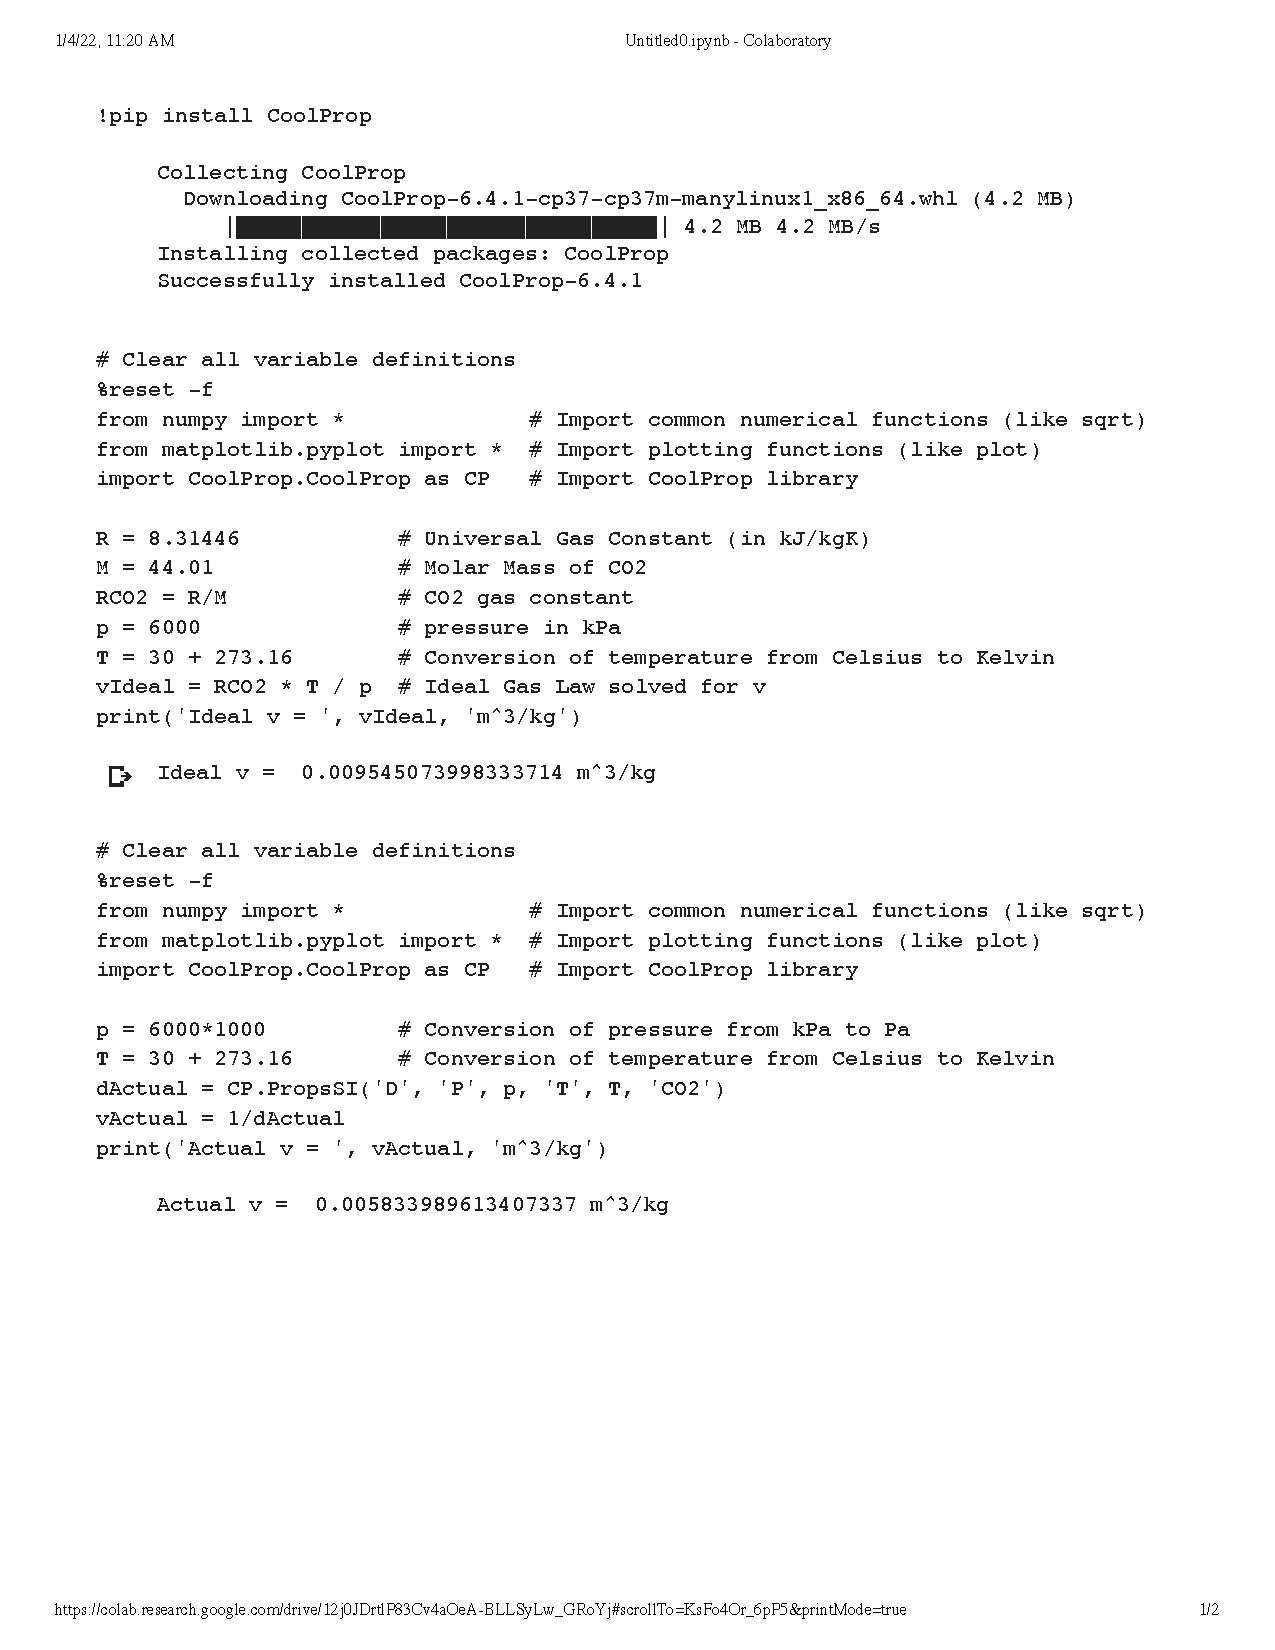
\includegraphics[width=0.75\textwidth]{ColabExample}
\caption{Output from Google Colab saved as a PDF.}
\label{fig:ch2_Colab}
\end{figure}


% --------------------------------------------------------------------
\section{Summary}
% --------------------------------------------------------------------

In this chapter, we determined the state of matter, which was determined by two independent properties, and then used that state to determine any missing properties.  As part of this process, we introduced linear interpolation to find values from the table that are not explicitly listed.  We also considered a number of processes, which are simply the change between two states.

Finally, we looked at two alternatives to the steam tables: the ideal gas law and software.  The ideal gas law requires a lot more calculation, but can be used when the steam tables are not available (which is typically the case).  Most importantly, a compressibility correction is necessary for low temperatures and/or high pressures.  Software can be used in most circumstances, but experience in coding is necessary to obtain accurate solutions.

\begin{homework}
  %--------------------------------------------------------------------
  \question How many independent quantities are necessary to fully describe a state of matter?
  %--------------------------------------------------------------------
  \question Define the following: phase, state, property, process
  %--------------------------------------------------------------------
  \question Two kilograms of water at 25°C are placed in a piston cylinder device under 3.2 MPa pressure. Heat is added to the water at constant pressure until the temperature of the fluid reaches 350°C (State (2)). Determine the final volume of the fluid at state (2). $\answer{[0.08508\ {\rm m^3}/{\rm kg}]}$
   %--------------------------------------------------------------------
  \question A piston-cylinder device contains a saturated mixture of steam and water having a total mass of 0.5 kg at a pressure of 160 kPa and an initial volume of 100 liters. Heat is then added and the fluid expands at constant pressure until it reaches a saturated vapor state.
\begin{questionparts}
\item Draw a diagram representing the process showing the initial and final states of the system.

\item Sketch this process on a P-v diagram with respect to the saturation lines, critical point, and relevant constant temperature lines, clearly indicating the initial and final states.

\item Determine the initial quality and temperature of the fluid mixture prior to heating. {\color{red} [$x_1$ = 0.182, $T_1$ = 113.3°C]}

\item Determine the final volume of the steam after heating. {\color{red} [0.546 $\rm m^3$ (546 liters)]}
\end{questionparts}
%--------------------------------------------------------------------
\question A pressure cooker allows much faster (and more tender) cooking by maintaining a higher boiling temperature of the water inside. It is well sealed, and steam can only escape through an opening on the lid, on which sits a metal petcock. When the pressure overcomes the weight of the petcock, the steam escapes, maintaining a constant high pressure while the water boils.

\begin{center}
  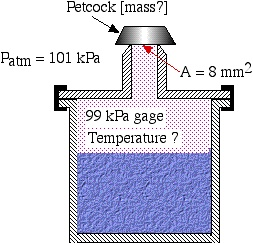
\includegraphics[width=0.4\textwidth]{press_cooker}
\end{center}
  
Assuming that the opening under the petcock has an area of 8 $\rm mm^2$, determine:

\begin{questionparts}
\item the mass of the petcock required in order to maintain an operating pressure of 99 kPa gauge. {\color{red}[80.7 g]}

\item the corresponding temperature of the boiling water. {\color{red}[120.2°C]}
\end{questionparts}
Note: Assume that the atmospheric pressure is 101 kPa. Draw a free body diagram of the petcock.

%--------------------------------------------------------------------
\question Consider a rigid container having a volume of 100 liters, filled with steam at an initial state of 400 kPa and 300°C. The steam is then cooled until it reaches a temperature of 90°C.

\begin{questionparts}
\item Draw a diagram representing the process showing the initial and final states of the system.

\item Using steam tables determine the mass of steam in the container. {\color{red} [0.153 kg]}

\item Using the ideal gas equation of state determine the mass of steam in the container. {\color{red} [0.151 kg]}
Determine the percentage error of using this method compared to that of using the steam tables. {\color{red}[1\%]}

\item Sketch this process on a $T$-$v$ (temperature-specific volume) diagram with respect to the saturation lines, critical point, and relevant constant pressure lines, clearly indicating the initial and final states.

\item Using steam tables determine the final pressure and quality of the fluid mixture after cooling. {\color{red}[70.2 kPa, $x$ = 0.277]}
\end{questionparts}
Note: The critical point data and ideal gas constant for steam can be found on the first page of the steam tables.

%--------------------------------------------------------------------

\question An automobile tire with a volume of 100 liters is inflated to a gauge pressure of 210 kPa. Determine:
\begin{questionparts}
\item the mass of air in the tire if the temperature is 20°C {\color{red} [$m$ = 0.369 kg]}
\item the increase in gauge pressure if the temperature in the tire reaches 50°C \\{\color{red} [$p_{2,gage}=$242 kPa]}
\end{questionparts}
Assume that atmospheric pressure is 100 kPa.

%--------------------------------------------------------------------

\question Compressed air is commonly used to power a large variety of power tools.  Lowe's sells an air compressor that can fill an 8-gallon tank to 160 psi. At a temperature of 70°F, determine the mass of the air inside a full 8-gallon tank.  Let $p_{atm} = 14.7$ psi.
\begin{questionparts}

\item Use the ideal gas law (you will need to do a lot of unit conversions for this). \\{\color{red} [0.429 kg]}

\item Find the compressibility factor.  How far off is your analysis above? {\color{red} [0.99]}

\end{questionparts}
\end{homework}



\chapter{The First Law for Closed Systems} \label{ch:closed_systems}
% --------------------------------------------------------------------
\section{Introducing the First Law}
% --------------------------------------------------------------------
The First Law of Thermodynamics states that energy is conserved (i.e. neither created nor destroyed).  As we discussed in Section \ref{sec:ch1_energyForms}, we can consider many types of energy (potential, kinetic, chemical, nuclear, and internal), but most of those are either small compared to internal (such as potential and kinetic) or outside the scope of this class (nuclear and chemical).

Energy can be transferred between the system and the surroundings in the form of heat and work, resulting in a change of internal energy of the system. Internal energy change can be considered as a measure of molecular activity associated with change of phase or temperature of the system.

The statement of the first law for closed systems reflects that we are primarily interested in the internal energy ($U$), heat transfer ($Q$), and work ($W$).
\begin{equation} \label{eq:1stLawClosed}
  Q - W = \Delta U
\end{equation}

\begin{figure}[H]
\centering
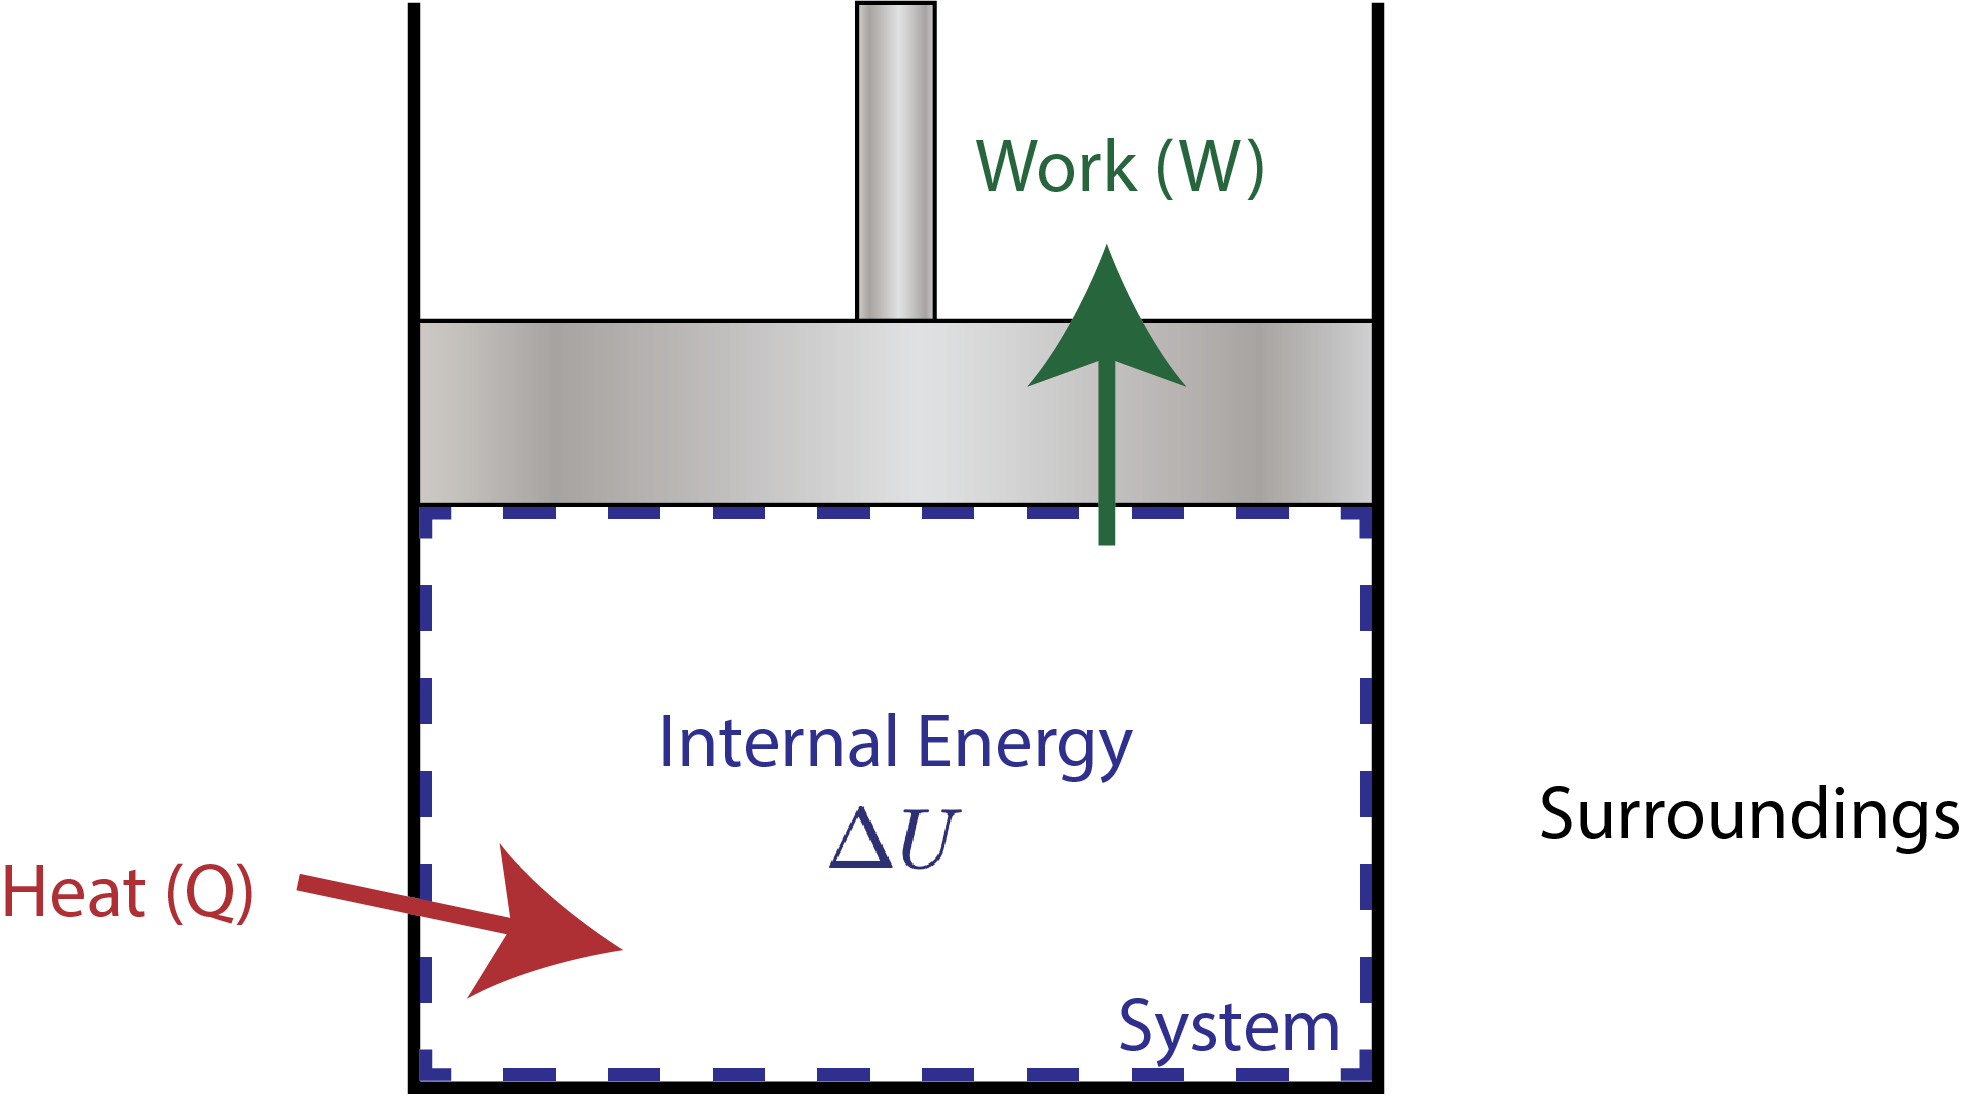
\includegraphics[width=0.5\textwidth]{FirstLaw}
\caption{A closed system with heat transfer and work.}
\label{fig:ch2_energyEquation}
\end{figure}

We can also write the first law by reducing each value to their {\bf mass-specific} counterparts.  Thus, $Q$ becomes $mq$, where $q$ is the mass-specific heat transfer.  $W$ becomes $mw$, where $w$ is the mass-specific work.  $U$ becomes $mu$, where $u$ is the mass-specific internal energy.  As a general rule, a capital variable refers to the extensive value, while the lower-case variable refers to an intensive value (mass is the biggest exception).

After we divide through by mass ($m$), the first law therefore becomes:
\begin{equation*}
  q - w = \Delta u
\end{equation*}

% --------------------------------------------------------------------
\subsection{Heat Transfer ($Q$)}
Energy transferred across the boundary of a system in the form of heat always results from a difference in temperature between the system and its immediate surroundings.  Heat transfer can occur through conduction, convection, or radiation.

{\bf Conduction} is the transfer of heat through direct contact.  When you touch an object hotter than your skin (a stove top, food heated in the oven, etc.), energy moves from the hot object to your colder skin.  The same occurs in reverse when you touch an object colder than your skin.  You typically perceive the movement of heat (not the temperature of the object itself).

{\bf Convection} is the transfer of heat through contact with a moving fluid, such as air or water.  Still air typically feels warmer than moving air (even when both are the same temperature) because the rate of heat transfer is higher.  This leads to the concept of ``wind chill'' in North America, the ``apparent temperature'' in Australia, among others.  These models attempt to show how windy days feel colder than a thermometer reading would indicate.  The \href{https://en.wikipedia.org/wiki/Wind_chill}{wind chill} is calibrated so that the rate of heat transfer is the same between a person walking in the windy weather and on a still day at the wind chill temperature.  The increased heat transfer from convection is also why fans can make a room feel cooler, even if they don't decrease the temperature.

{\bf Radiation} is the transfer of heat through the absorption of light.  Photons are emitted from all substances above absolute zero, and these photons carry energy.  You feel the heat of a fire not through contact with the superheated air, but because the air is hot enough to emit a significant amount of light in the infrared and visible spectrums, which is then absorbed by your skin.  Likewise, you can feel the heat of the sun because the photons are able to travel through the vacuum of space.

The calculation of heat transfer due to temperature differences is left for a later class.  In this book, the quantity of heat transferred during any process will either be specified as part of the problem or evaluated as the unknown of the energy equation.

By convention, {\bf heat is that transferred into the system from the surroundings is considered positive}. Positive heat transfer results in an increase in internal energy of the system.

Heat transfer is {\bf path-dependent} and not a property. It is dependent on the process path between the initial and final states.

Recall in Section \ref{sec:ch1_process} that we introduced some commonly used processes:
\begin{itemize}
\item Isothermal (constant temperature process)
\item Isochoric or isometric (constant volume process)
\item Isobaric (constant pressure process)
\item Adiabatic (no heat flow to or from the system during the process)
\end{itemize}

% --------------------------------------------------------------------
\subsection{Work ($W$)}
%In this course we consider three modes of work transfer across the boundary of a system, as shown in the following diagram:

%\begin{figure}[H]
%\centering
%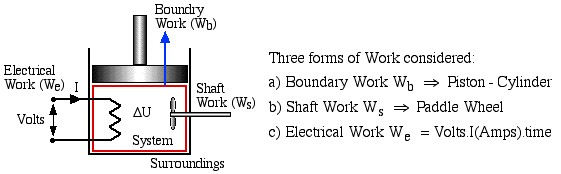
\includegraphics[width=0.75\textwidth]{Work}
%\caption{Description of three types of work.}
%\label{fig:ch2_work}
%\end{figure}

In this course we are primarily concerned with {\bf boundary work} due to compression or expansion of a system in a piston-cylinder device as shown above. In all cases we assume a perfect seal (no mass flow in or out of the system), no loss due to friction, and quasi-equilibrium processes in that for each incremental movement of the piston equilibrium conditions are maintained.

By convention positive work is that done by the system on the surroundings, and negative work is that done by the surroundings on the system.  Since negative work results in an increase in internal energy of the system, this explains the negative sign in Equation \ref{eq:1stLawClosed}.

Boundary work is evaluated by integrating the force $F$ multiplied by the incremental distance moved $dx$ between an initial state (1) to a final state (2). We normally deal with a piston-cylinder device, thus the force can be replaced by the piston area $A$ multiplied by the pressure $p$, allowing us to replace $A\:dx$ by the change in volume $dV$, as follows:

\begin{equation} \label{eq:ch3_work}
  W_{1-2}=\int_1^2F\:dx=\int_1^2pA\:dx=\int_1^2p\:dV=m\int_1^2 p\:dv
\end{equation}

Figure \ref{fig:ch3_pV} provides an example of a piston being compressed.  However, until the process path is specified, it is impossible to know how much work is associated with the compression.  This is seen in the figure as each process has a different area under the curve, which is directly related to the integral in Equation \ref{eq:ch3_work}.  In other words, work done is {\bf path-dependent} and not a property, exactly like heat transfer.

\begin{figure}[H]
\centering
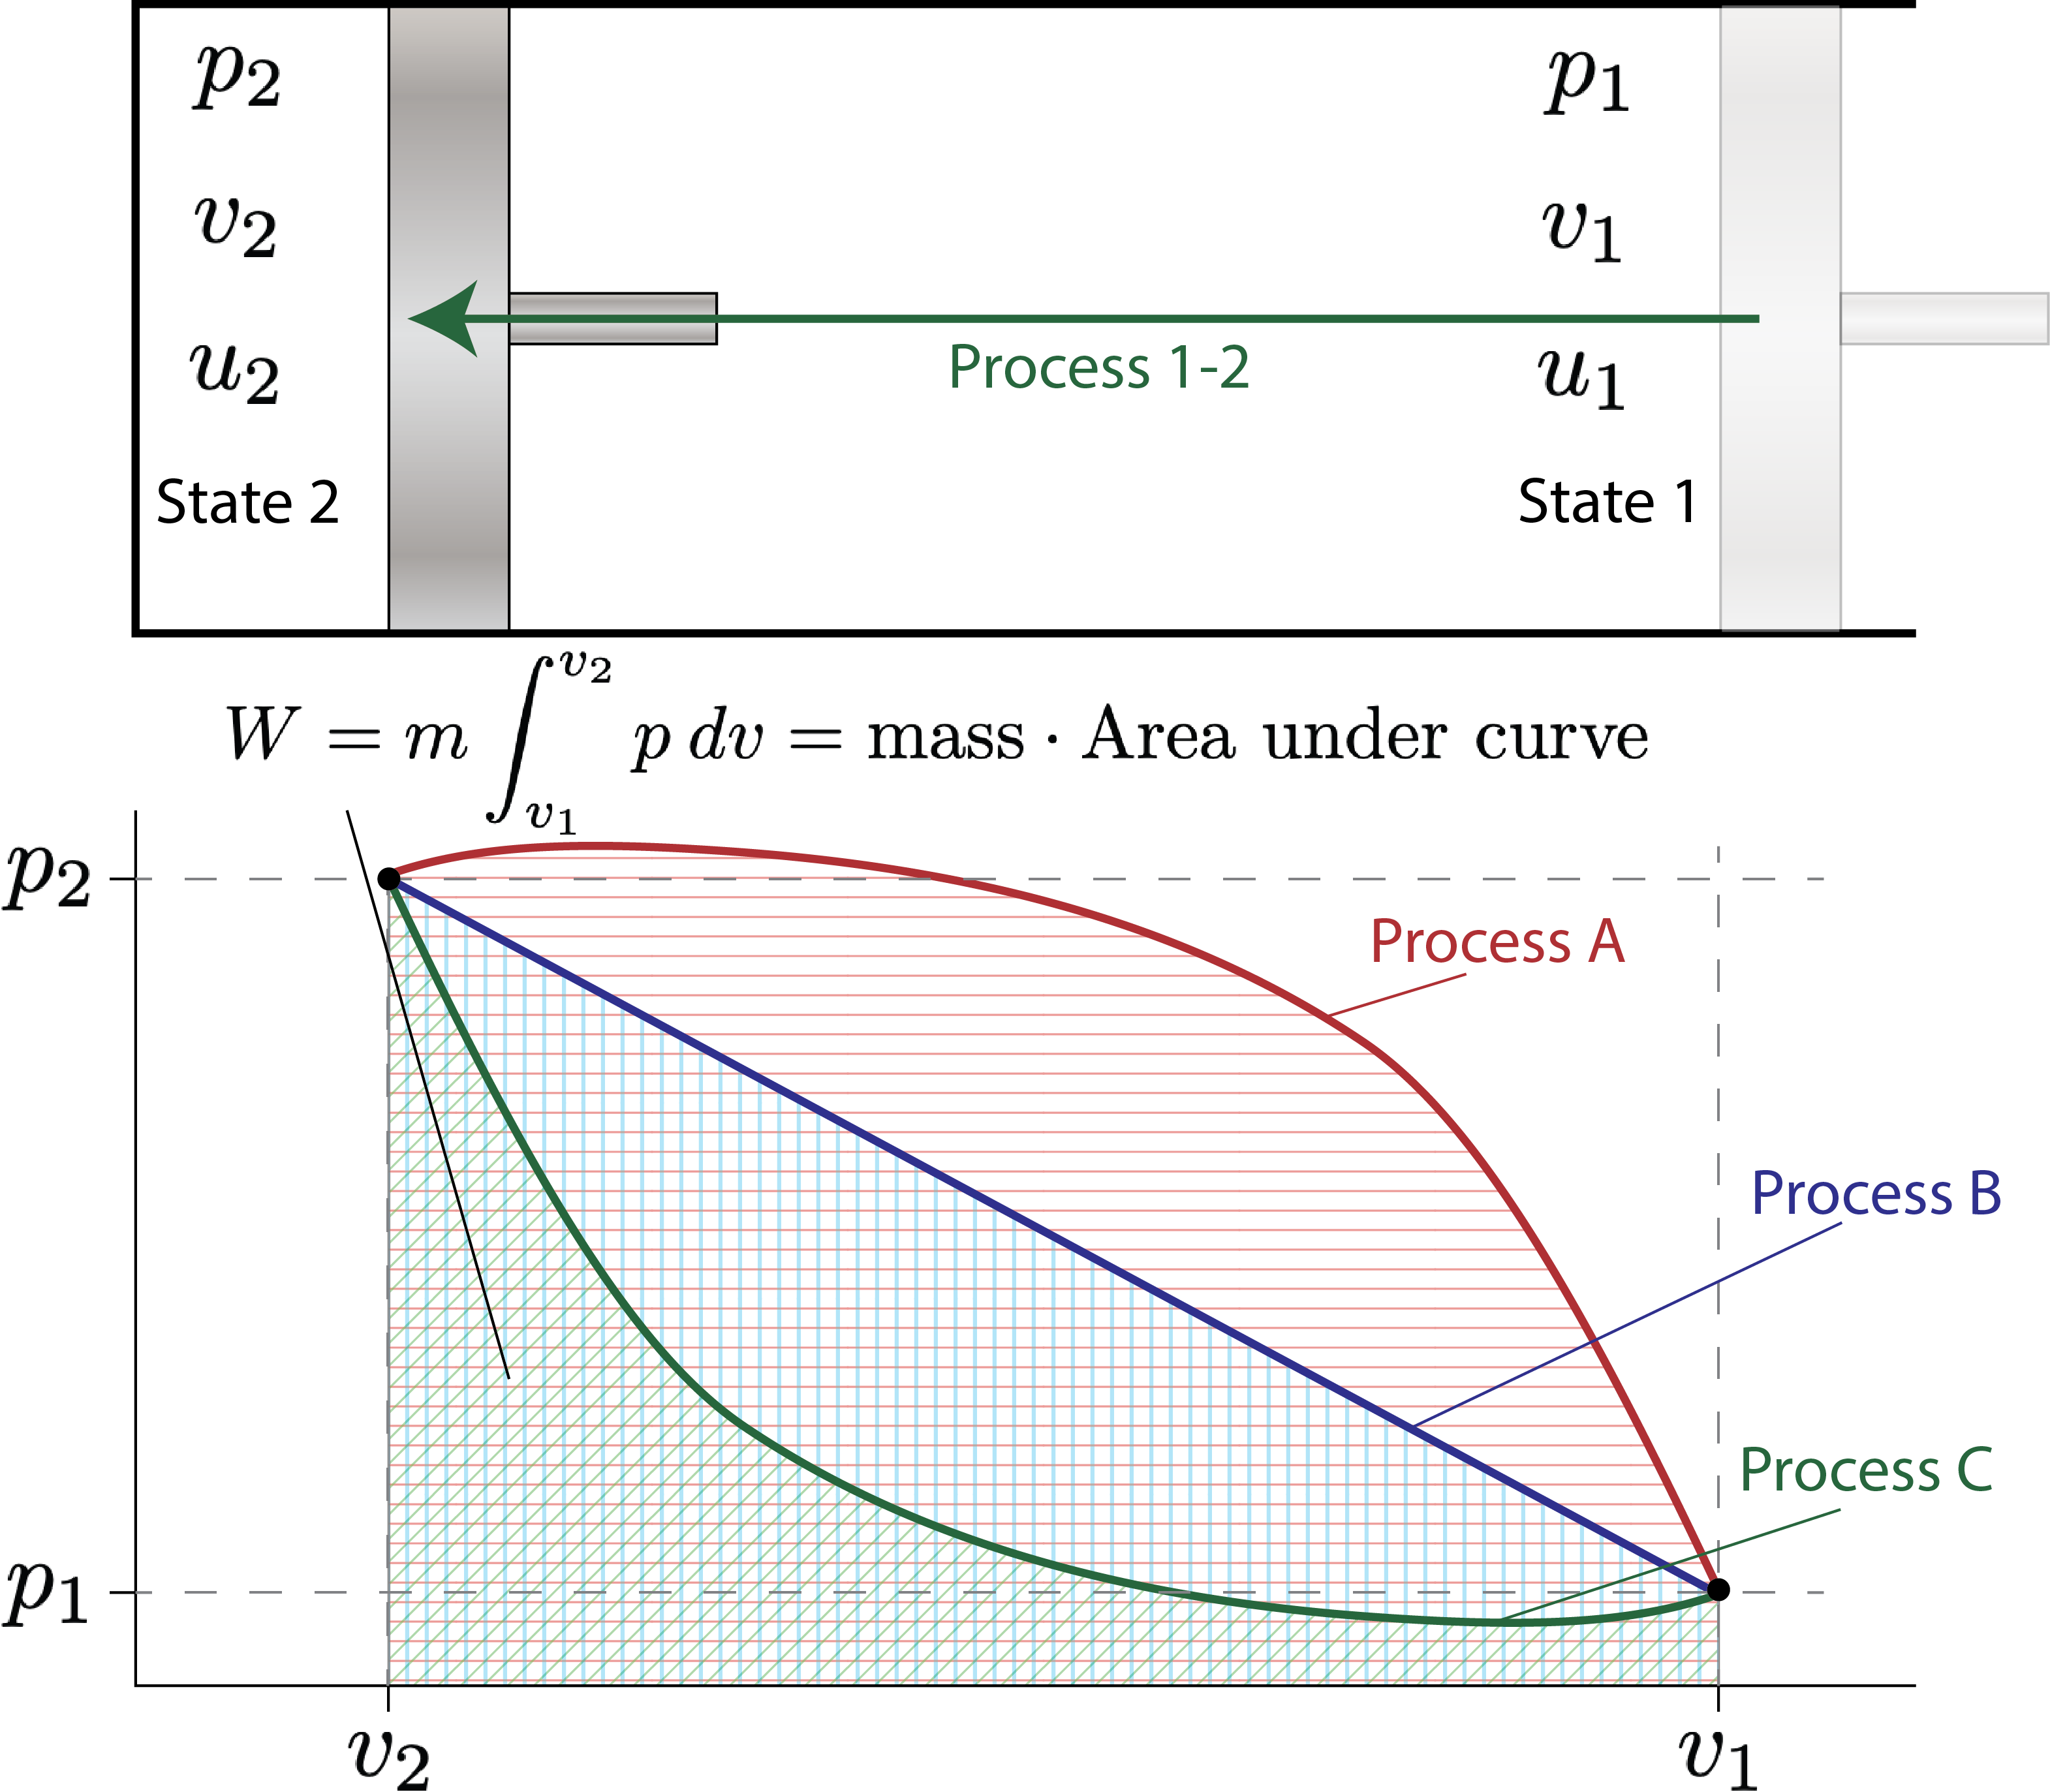
\includegraphics[width=0.75\textwidth]{processWork}
\caption{The state of a piston plotted as air is compressed.  Multiple paths can be taken to connect the same two states.  Processes A, B, and C will have different amounts of work and heat transfer associated with them.}
\label{fig:ch3_pV}
\end{figure}

We note that work done by the system on the surroundings (expansion process) is positive, and that done on the system by the surroundings (compression process) is negative.

Finally, {\bf shaft work} (due to a paddle wheel) and {\bf electrical work} (due to a voltage applied to an electrical resistor or motor driving a paddle wheel) will always be negative (work done on the system). Positive forms of shaft work, such as that due to a turbine, will be considered in Chapter 4 when we discuss open systems.


% --------------------------------------------------------------------
\subsection{Internal Energy ($\Delta U$)}

The third component of Equation \ref{eq:1stLawClosed} is the change of internal energy. Recall from Section \ref{sec:ch1_internalEnergy} that internal energy is closely tied to the temperature of a substance.  In fact, specific internal energy is a property of the system, like temperature and pressure.  From the State Postulate, we can find the internal energy of a state as long as we know at least two other properties.

Often, we prefer to use the mass-specific form of internal energy, which is related to the internal energy in our system as follows:
\begin{equation*}
  u = \frac{U}{m} \quad \rightarrow \quad \Delta u = \frac{\Delta U}{m}
\end{equation*}

Internal energy can be determined from the steam tables in Appendix \ref{ch:appendixSteam} or the R134a tables in Appendix \ref{ch:appendixR134a}.
Heat transfer and work cannot be found from tables because they are not a property of a state, but rather a description of how a process moves between states.

Example \ref{ex:constantPressureRevisited} makes use of the First Law to calculate the heat transfer for a constant pressure process.

\begin{example}[label={ex:constantPressureRevisited}]{Constant Pressure Expansion Revisited}
  Recall Example \ref{ex:ch2constantPressure} in which we presented a constant pressure process. We wish to extend the problem to include the energy interactions of the process, hence we restate it as follows:

  Two kilograms of water at 25°C are placed in a piston cylinder device under 3.2 MPa pressure as shown in the diagram (State (1)). Heat is added to the water at constant pressure until the temperature of the steam reaches 350°C (State (2)).

  Determine the work done by the fluid ($W$) and heat transferred to the fluid ($Q$) during this process.\\

  {\bf Solution Approach}
  We first draw the diagram of the process including all the relevant data as follows:

\begin{center}
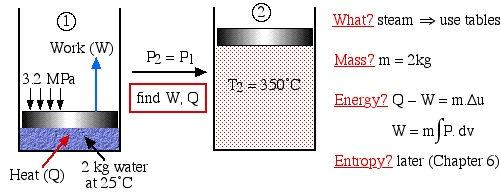
\includegraphics[width=0.75\textwidth]{example3-1}
%\captionof{figure}{}
%\label{fig:ch2_example1}
\end{center}

Notice the four questions to the right of the diagram, which we should always ask before attempting to solve any thermodynamic problem.

\begin{itemize}
  \item {\bf What?} \\
What are we dealing with - liquid? pure fluid, such as steam or refrigerant? ideal gas? In this case it is steam, thus we will use the steam tables to determine the various properties at the various states.

\item {\bf Mass?} \\
Is the mass or volume given? If so we will specify and evaluate the energy equation in kiloJoules rather than specific quantities (kJ/kg).

\item {\bf Energy?}\\
  The energy equation will almost always be our starting point for working through these problems.

\item {\bf Entropy?}\\
What about entropy? Not so fast - wait until Chapter 6.
\end{itemize}
Since work involves the integral of $p\cdot dv$ we find it convenient to sketch the $p$-$v$ diagram of the problem as follows:

\begin{center}
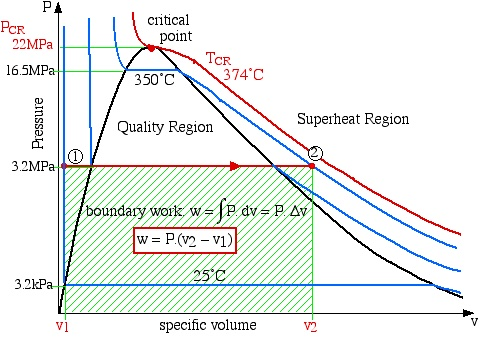
\includegraphics[width=0.75\textwidth]{example3-1_Pv}
%\captionof{figure}{}
%\label{fig:ch2_example1}
\end{center}

Notice on the $p$-$v$ diagram how we determine the specific work done as the area under the process curve. We also notice that in the compressed liquid region the constant temperature line is essentially vertical. Thus all the property values at State (1) (compressed liquid at 25°C) can be determined from the saturated liquid table values at 25°C.

\begin{align*}
  u_1 &= u_{f,\ 25°C}=104.8 \left[\frac{\rm kJ}{\rm kg}\right]\\
  v_1 &= v_{f,\ 25°C}=0.001 \left[\frac{\rm m^3}{\rm kg}\right]
\end{align*}

\begin{center}
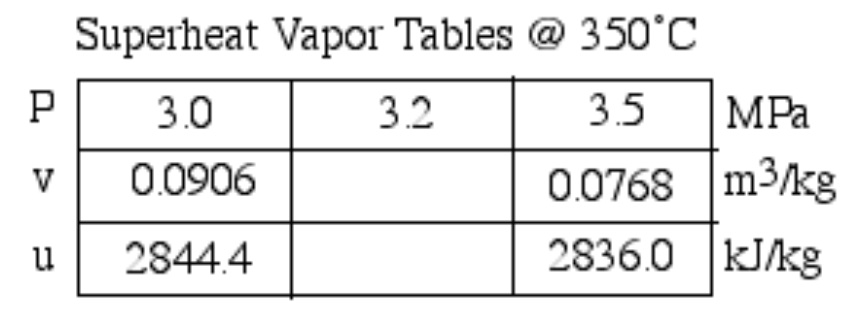
\includegraphics[width=0.5\textwidth]{example3-1_tables}
%\captionof{figure}{}
%\label{fig:ch2_example1}
\end{center}

\begin{align*}
  \frac{\Delta p_A}{\Delta p_b} = \frac{\Delta v_A}{\Delta v_b} &\rightarrow \frac{3.2 - 3.0}{3.5-3.0} = \frac{v_2-0.0906}{0.0768-0.0906} = 0.4\\
  v_2 &= 0.085 \frac{\rm m^3}{\rm kg} \\
  \frac{\Delta p_A}{\Delta p_b} = \frac{\Delta u_A}{\Delta u_b} &\rightarrow \frac{3.2 - 3.0}{3.5-3.0} = \frac{u_2-2844.4}{2836.0-2844.4} = 0.4\\
  u_2 &= 2841 \frac{\rm kJ}{\rm kg}
\end{align*}

Now we use $\Delta v$ to define our work:
\begin{align*}
  W = m \int p dv = m\cdot p \cdot \Delta v = 2.0\ {\rm kg} \cdot 3200\ {\rm kPa} \cdot (0.085 - 0.001)\ \frac{\rm m^3}{\rm kg} \\
  \redbox{W = 538\ {\rm kJ}}
\end{align*}
Then, with work and $\Delta U$, we can find our heat transfer:
\begin{align*}
  \Delta U = Q - W \rightarrow Q = m\cdot (u_2 - u_1) + W \\
  Q = 2.0\ {\rm kg} \cdot (2841 - 104.8)\ \frac{\rm kJ}{\rm kg} + 538\ {\rm kJ} \\
   \redbox{Q = 6010\ {\rm kJ}}
\end{align*}
\end{example}

% --------------------------------------------------------------------
\section{Enthalpy ($h$)- A New Property} \label{sec:ch3_enthalpy}
% --------------------------------------------------------------------

In the case studies that follow we find that one of the major applications of the closed system energy equation is in heat engine processes in which the system is approximated by an ideal gas, thus we will develop relations to determine the internal energy for an ideal gas. We will find also that a new property called {\bf enthalpy} will be useful both for closed systems and in particular for open systems, such as the components of steam power plants or refrigeration systems. Enthalpy is not a fundamental property. Instead, it is a combination of properties and is defined as follows:
\begin{equation}
  h = u + p\cdot v\quad \quad {\rm OR} \quad \quad H = U + p\cdot V
\end{equation}
As with other properties, the lowercase $h$ refers to the mass specific property and is measured in $\frac{\rm kJ}{\rm kg}$, whereas the capital $H$ is an extensive property and is measured in kJ.

Enthalpy shows its use whenever applied to a constant pressure process, such as Example \ref{ex:constantPressureRevisited}.  For these processes, work can be defined as $w = p\cdot \Delta v$, meaning that the energy equation can be written as:
\begin{align*}
  \Delta u &= q - p \Delta v\\
  u_2 - u_1 &= q - p\: (v_2 - v_1)\\
  (u_2 &+ p\: v_2) - (u_1 + p\: v_1) = q \\
  h_2 &- h_1 = q \rightarrow \redbox{q = \Delta h}
\end{align*}

This means that we can look up enthalpy directly to find heat transfer {\bf for constant pressure processes}.

% --------------------------------------------------------------------
\section{Specific Heats} \label{sec:specificHeats}
% --------------------------------------------------------------------

For solids and liquids, we can define a relatively simple equation:
\begin{equation} \label{eq:calorimetry}
  Q = mc\Delta T\quad\quad {\rm OR} \quad\quad q=c\Delta T
\end{equation}
The variable $c$ is called the {\bf specific heat}, and is a relationship between the amount of heat added to a material and the temperature increase we expect.  This is often discussed in chemistry alongside devices known as calorimeters.

% --------------------------------------------------------------------
\subsection{Constant Volume}
In this section, we will expand the concept of specific heat to gases.  To start, let's consider $u$ as a function of $T$ and $v$:
\begin{equation*}
  u = u(T, v)
\end{equation*}

Using the concept of the {\bf total differential} from Calculus, we can write:
\begin{equation*}
  du = \frac{\partial u}{\partial T}dT + \frac{\partial u}{\partial v}dv
\end{equation*}

Since a partial derivative only considers change from a single variable, and we assumed that $u$ was a function only of $T$ and $v$, $\partial u / \partial T$ is the same as saying ``the change of $u$ with respect to $T$ when $v$ is constant''.

However, we could have written $u$ as a function of any two independent properties, so to specify exactly which one, we'll add the property that stays constant as a subscript:
\begin{equation*}
  \frac{\partial u}{\partial T} = \left[\frac{d u}{d T}\right]_v
\end{equation*}

Writing $du$ again, we get:
\begin{equation}\label{eq:du_Tv}
  du = \left[\frac{d u}{d T}\right]_v dT + \left[\frac{d u}{d v}\right]_T dv
\end{equation}

Now, let's write the energy equation in differential form.  Recall that $w = p \Delta v$, which can be written in differential form as $\delta w = p\: dv$.
\begin{equation}\label{eq:differentialEnergy}
  \delta q - \delta w = du \quad \rightarrow \quad \delta q - p\: dv = du
\end{equation}

We used $\delta q$ and $\delta w$ because $q$ and $w$ are not properties, and therefore not integrable in the same way as $v$ and $u$.

Combining Equations \ref{eq:du_Tv} and \ref{eq:differentialEnergy}, we get:
\begin{equation*}
  \delta q = \left[\frac{d u}{d T}\right]_v dT + \left(\left[\frac{d u}{d v}\right]_T + p \right) dv
\end{equation*}

All of this leads to a huge simplification for constant-volume processes.  If $dv = 0$, we get the following:
\begin{equation} \label{eq:cv1}
  \delta q = \left[\frac{d u}{d T}\right]_v dT
\end{equation}

Equation \ref{eq:cv1} is simply the differential form of Equation \ref{eq:calorimetry}!  In fact, $\left[\frac{d u}{d T}\right]_v$ is simply the {\bf constant volume specific heat}, $c_v$.

% --------------------------------------------------------------------
\subsection{Constant Pressure}

Now we could have started this discussion by defining $h$ as a function of $T$ and $p$.
\begin{equation*}
  h = h(T, p)
\end{equation*}
That would result in:
\begin{equation}\label{eq:dh_Tp}
  dh = \left[\frac{d h}{d T}\right]_p dT + \left[\frac{d h}{d p}\right]_T dp
\end{equation}
We know that the second half will eventually fall off when we think about constant pressure systems.

Let's expand $dh$, using our definition of $h=u + pv$.  In order to do so, we need to remember the Product Rule from Calculus: $(fg)' = f'g + g'f$
\begin{align}
  \nonumber dh &= d(u + pv) = du + d(pv) \\
  \label{eq:dhExpanded} dh &= du + p\: dv + v\: dp
\end{align}

Now, we can replace $du$ with $\delta q - p\: dv$, based on Equation \ref{eq:differentialEnergy}:
\begin{align*}
  dh &= (\delta q - p\: dv) + p\: dv + v\: dp \\
  dh &= \delta q + v\: dp
\end{align*}

Next, we plug our result into Equation \ref{eq:dh_Tp}:
\begin{align*}
  \delta q + v\: dp &= \left[\frac{d h}{d T}\right]_p dT + \left[\frac{d h}{d p}\right]_T dp \\
  \delta q &= \left[\frac{d h}{d T}\right]_p dT + \left(\left[\frac{d h}{d p}\right]_T  - v \right)dp
\end{align*}

Finally, we implement the constant pressure assumption, which sets $dp=0$:
\begin{equation} \label{eq:cp1}
  \delta q = \left[\frac{d h}{d T}\right]_p dT
\end{equation}

Again, with Equation \ref{eq:cp1}, we can state that $\left[\frac{d h}{d T}\right]_p$ is the {\bf constant pressure specific heat}, $c_p$.

% --------------------------------------------------------------------
\subsection{Ideal Gases}
Now, consider $u$ and $h$ for ideal gases.  We state without proof that for an ideal gas, internal energy depends on temperature alone.  In other words, $u$ and $c_v$ are purely functions of temperature.

With $u=u(T)$ and $pv = RT$, we can write:
\begin{equation*}
  h = u + pv = u(T) + RT
\end{equation*}

This means that $h$ is also only a function of temperature!  In fact, by evaluating $d h/d T$, we can say:
\begin{equation} \label{eq:ch3_cpcvR}
  \frac{d h}{d T} = \frac{d u}{d T} + R \quad\rightarrow\quad c_p = c_v + R
\end{equation}

Because both $c_p$ and $c_v$ are only functions of temperature, we can drastically reduce the amount of information needed for the tables.  A single table (Appendix \ref{sec:idealGasAir}) is sufficient for all ideal gas properties. In fact, we can even assume a constant specific heat and retain good accuracy, as long as the specific heat is evaluate at the average temperature, $T_{avg}$.

\begin{equation}
  \Delta u = c_v(T_{avg})\cdot \Delta T  \quad \quad\quad \Delta h = c_p(T_{avg})\cdot \Delta T
\end{equation}

\begin{example}{Ideal Gas $u$ and $h$}
  Air at 300 K undergoes a process in which heat is added at constant pressure.  Consider processes that end at 900 K, 1200 K, and 1500 K.
  Determine the heat added using a) $c_p(T_{avg})$ and b) the enthalpies given in the table.

  {\bf Solution Approach}
  Since the process occurs at constant pressure, we know that the heat added is simply the difference in enthalpy:
  \begin{equation*}
    Q = h_2 - h_1
  \end{equation*}

  If we assume constant specific heat, we can also say that:
  \begin{equation*}
    Q = c_p \left(T_2 - T_1\right)
  \end{equation*}

  \begin{enumerate}[a)]
  \item We first need to find the $c_p$ at the average process temperatures.
    \begin{center}
      \begin{tabular}{ccc}
        $T_2$ & $T_{avg}$ & $c_p(T_{avg})$ \\ \hline
        900 K & 600 K & 1.0509 kJ/kgK \\
        1200 K & 750 K & 1.0866 kJ/kgK \\
        1500 K & 900 K & 1.1208 kJ/kgK
      \end{tabular}
    \end{center}
    Note that we needed to use linear interpolation in order to find the $c_p$ at 750 K.

    With the $c_p$ values in hand, we can find $Q$:
    \begin{center}
      \begin{tabular}{cccc}
        $T_2$ & $\Delta T$ & $c_p(T_{avg})$ & $Q$\\ \hline
        900 K & 600 K & 1.0509 kJ/kgK & 630.54 kJ/kg\\
        1200 K & 900 K & 1.0866 kJ/kgK & 977.94 kJ/kg\\
        1500 K & 1200 K & 1.1208 kJ/kgK & 1344.96 kJ/kg
      \end{tabular}
    \end{center}
    The rightmost column above is our desired result.
  \item The second method requires us to find the enthalpies directly.  The enthalpy of air at 300 K is 426.53 kJ/kg.  The enthalpies at the end of the process, along with the resulting heat transfers, are given below:
    \begin{center}
      \begin{tabular}{ccc}
        $T_2$ & $h_2$ & $Q$ \\ \hline
        900 K & 1059.36 kJ/kg & 632.83 kJ/kg \\
        1200 K & 1404.14 kJ/kg & 977.61 kJ/kg \\
        1500 K & 1762.29 kJ/kg & 1335.76 kJ/kg
      \end{tabular}
    \end{center}
    Again, the rightmost column is our desired result.
  \end{enumerate}
  Comparing the two methods, we can find the percent error through the formula:
  \begin{equation*}
    err = \frac{Q_a-Q_b}{Q_b} \times 100 \%
  \end{equation*}
  Finally, we see the errors below:
  \begin{center}
      \begin{tabular}{cc}
        $T_2$ & Error \\ \hline
        900 K & -0.36\%\\
        1200 K & 0.034\% \\
        1500 K & 0.69\%
      \end{tabular}
  \end{center}
  In all three cases, we see less than 1\% error, meaning that the average $c_p$ method is very accurate for air.
\end{example}
\newpage
% --------------------------------------------------------------------
\section{Stirling Cycle Engine} \label{sec:ch3_stirling}
% --------------------------------------------------------------------
\label{sec:idealStirling}
Conceptually, the Stirling engine, invented by Robert Stirling, is the simplest of all heat engines. It has no valves, and includes an externally heated space and an externally cooled space. 

In its original form the working gas (typically air or helium) is sealed within a single cylinder by the piston and shuttled between the hot and cold spaces by a displacer, as seen in Figure \ref{fig:ch3_stirlingAll}. The linkage driving the piston and displacer will move them such that the gas will compress while it is mainly in the cool compression space and expand while in the hot expansion space. This is clearly illustrated in \href{https://en.wikipedia.org/wiki/Stirling_engine#/media/File:Stirling_Animation.gif}{this animation} which was produced by Richard Wheeler (Zephyris) of Wikipedia.

\begin{figure}[H]
\centering
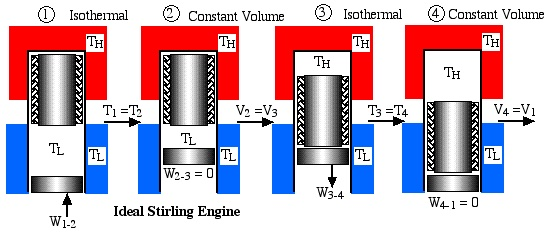
\includegraphics[width=0.75\textwidth]{StirlingEngine}
\caption{The states of the Stirling engine cycle.}
\label{fig:ch3_stirlingAll}
\end{figure}
Refer also to the \href{http://animatedengines.com/stirling.html}{animation produced by Matt Keveney} in his Stirling engine animation website. Since the gas is at a higher temperature, and therefore pressure, during its expansion than during its compression, more power is produced during expansion than is reabsorbed during compression, and this net excess power is the useful output of the engine. Note that there are no valves or intermittent combustion, which is the major source of noise in an internal combustion engine. The same working gas is used over and over again, making the Stirling engine a sealed, closed cycle system. All that is added to the system is steady high temperature heat, and all that is removed from the system is low temperature (waste) heat and mechanical power.

Please note that the following analysis of Stirling cycle engines is ideal, and is intended only as an example of First Law Analysis of closed systems. In the real world we cannot expect actual machines to perform any better than 40 - 50\% of the ideal machine.
%The analysis of actual Stirling cycle machines is extremely complex and requires sophisticated computer analysis (see for example the web learning resource on: \href{https://www.ohio.edu/mechanical/stirling/index.html}{Stirling Cycle Machine Analysis}).

The four states of the Stirling engine are summarized in Figure \ref{fig:ch3_stirlingAll} and Figure \ref{fig:ch3_stirlingDiagram}.  Note specifically the motion of both the piston and the displacer.  The movement of the piston correlates to the compression or expansion of the fluid, while the action of the displacer is to move the fluid between the hot and cold regions, thereby heating or cooling the fluid.

In essence, the ideal Stirling engine undergoes four distinct processes, each of which can be analyzed separately: isothermal compression at $T_C$, constant volume heating at $v_{min}$, isothermal expansion at $T_H$, and constant volume cooling (or heat rejection) at $v_{max}$.

\begin{figure}[H]
\centering
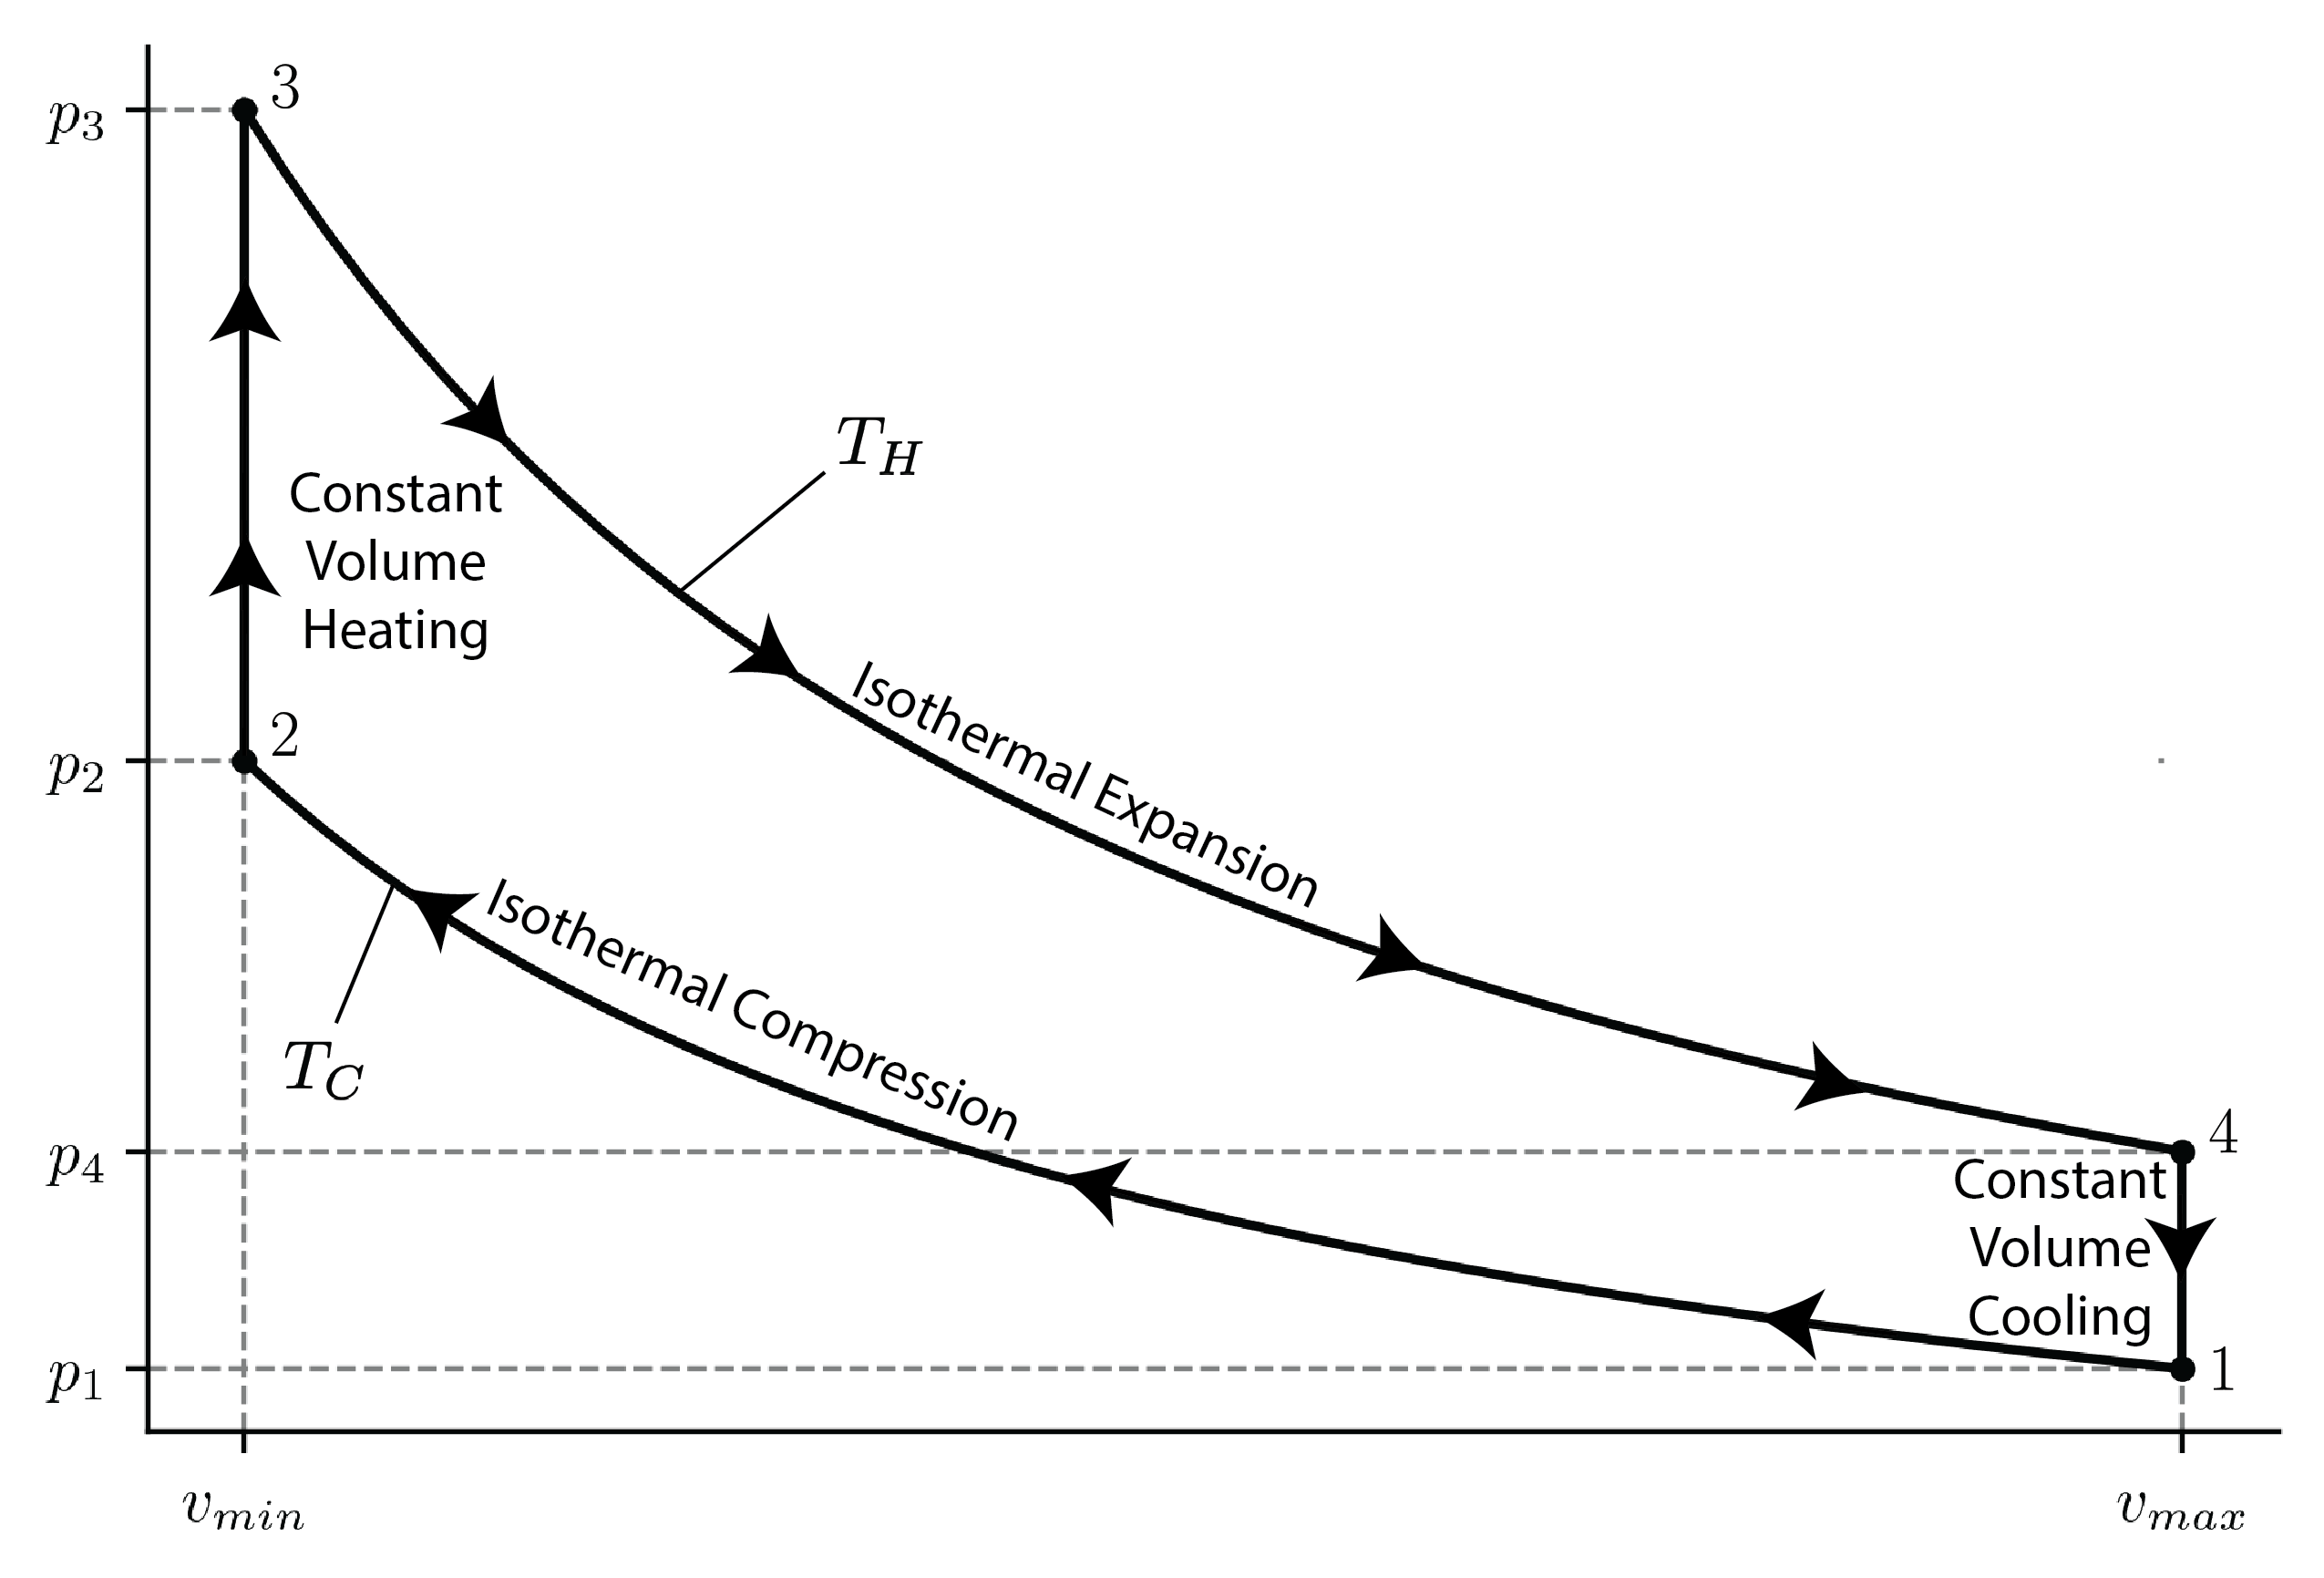
\includegraphics[width=0.75\textwidth]{StirlingDiagram}
\caption{The states of the Stirling engine cycle.}
\label{fig:ch3_stirlingDiagram}
\end{figure}

% --------------------------------------------------------------------
\subsection{Process 1$\rightarrow$2 -- Isothermal Compression}
We start our analysis at State 1, which is the coolest and least compressed point of the cycle.

\begin{figure}[H]
\centering
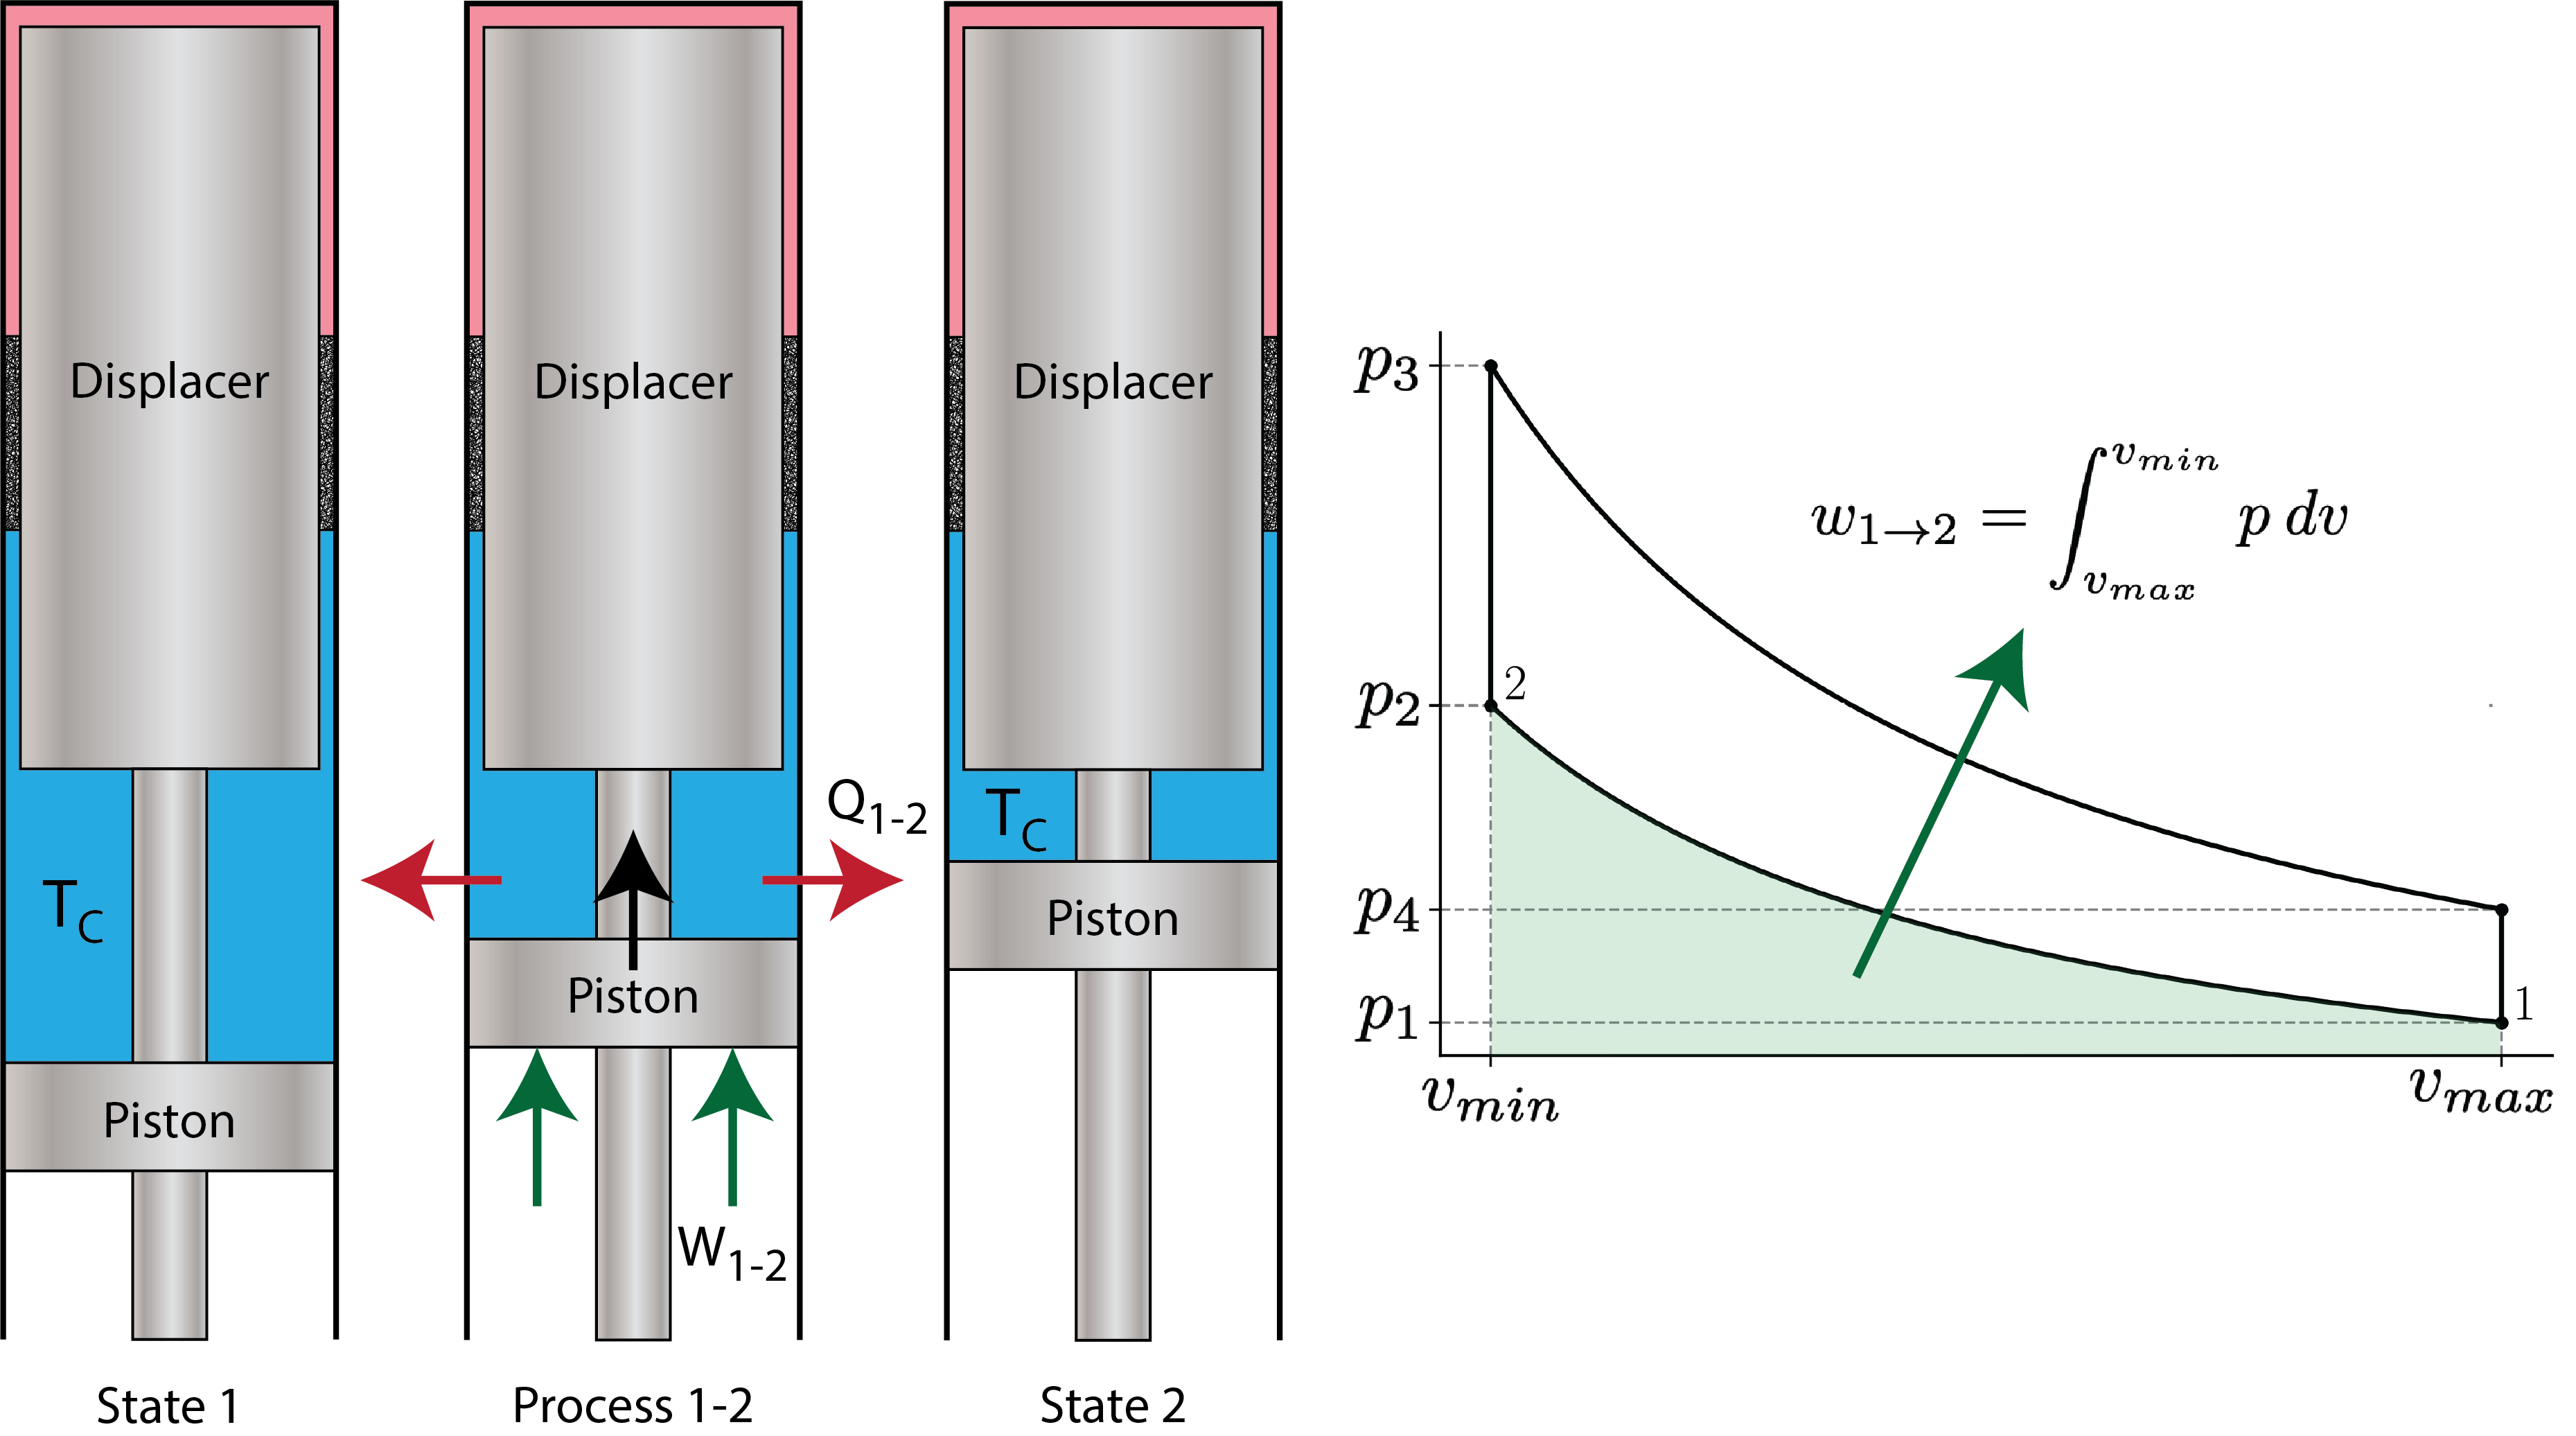
\includegraphics[width=0.9\textwidth]{StirlingEngineProcess1-2}
\caption{The compression process of the Stirling Engine.}
\label{fig:ch3_stirling12}
\end{figure}

Figure \ref{fig:ch3_stirling12} shows the compression from State 1 to State 2.  In process 1-2, the gas is compressed by the piston while the displacer is at the top of the cylinder. Thus during this process the gas is cooled in order to maintain a constant temperature $T_C$.  Note that without cooling, the work added by compression would increase the internal energy, and by extension temperature.

The work $W_{1-2}$ required to compress the gas is shown as the area under the $p$-$V$ curve, and is evaluated as follows, using the ideal gas law with the constant temperature during compression to say $p = \frac{R T_C}{v}$.

\begin{equation} \label{eq:stirlingCompWork}
  w_{1-2} = \int_{v_1}^{v_2} p\:dv=R T_C \int_{v_1}^{v_2} \frac{dv}{v}=RT_C\cdot  \ln\left(\frac{v_2}{v_1}\right)
\end{equation}

Another consequence of the constant temperature is that the internal energy of the gas will also stay unchanged.

\begin{equation}
  q_{1-2} - w_{1-2} = \cancelto{0}{\Delta u_{1-2}} \quad \rightarrow \quad q_{1-2} = w_{1-2}
\end{equation}

% --------------------------------------------------------------------
\subsection{Process 2$\rightarrow$3 -- Constant Volume Heating}

After compression, the displacer piston pushes the air from the cold region to the hot region, warming it up as it moves through the regeneration matrix.

\begin{figure}[H]
\centering
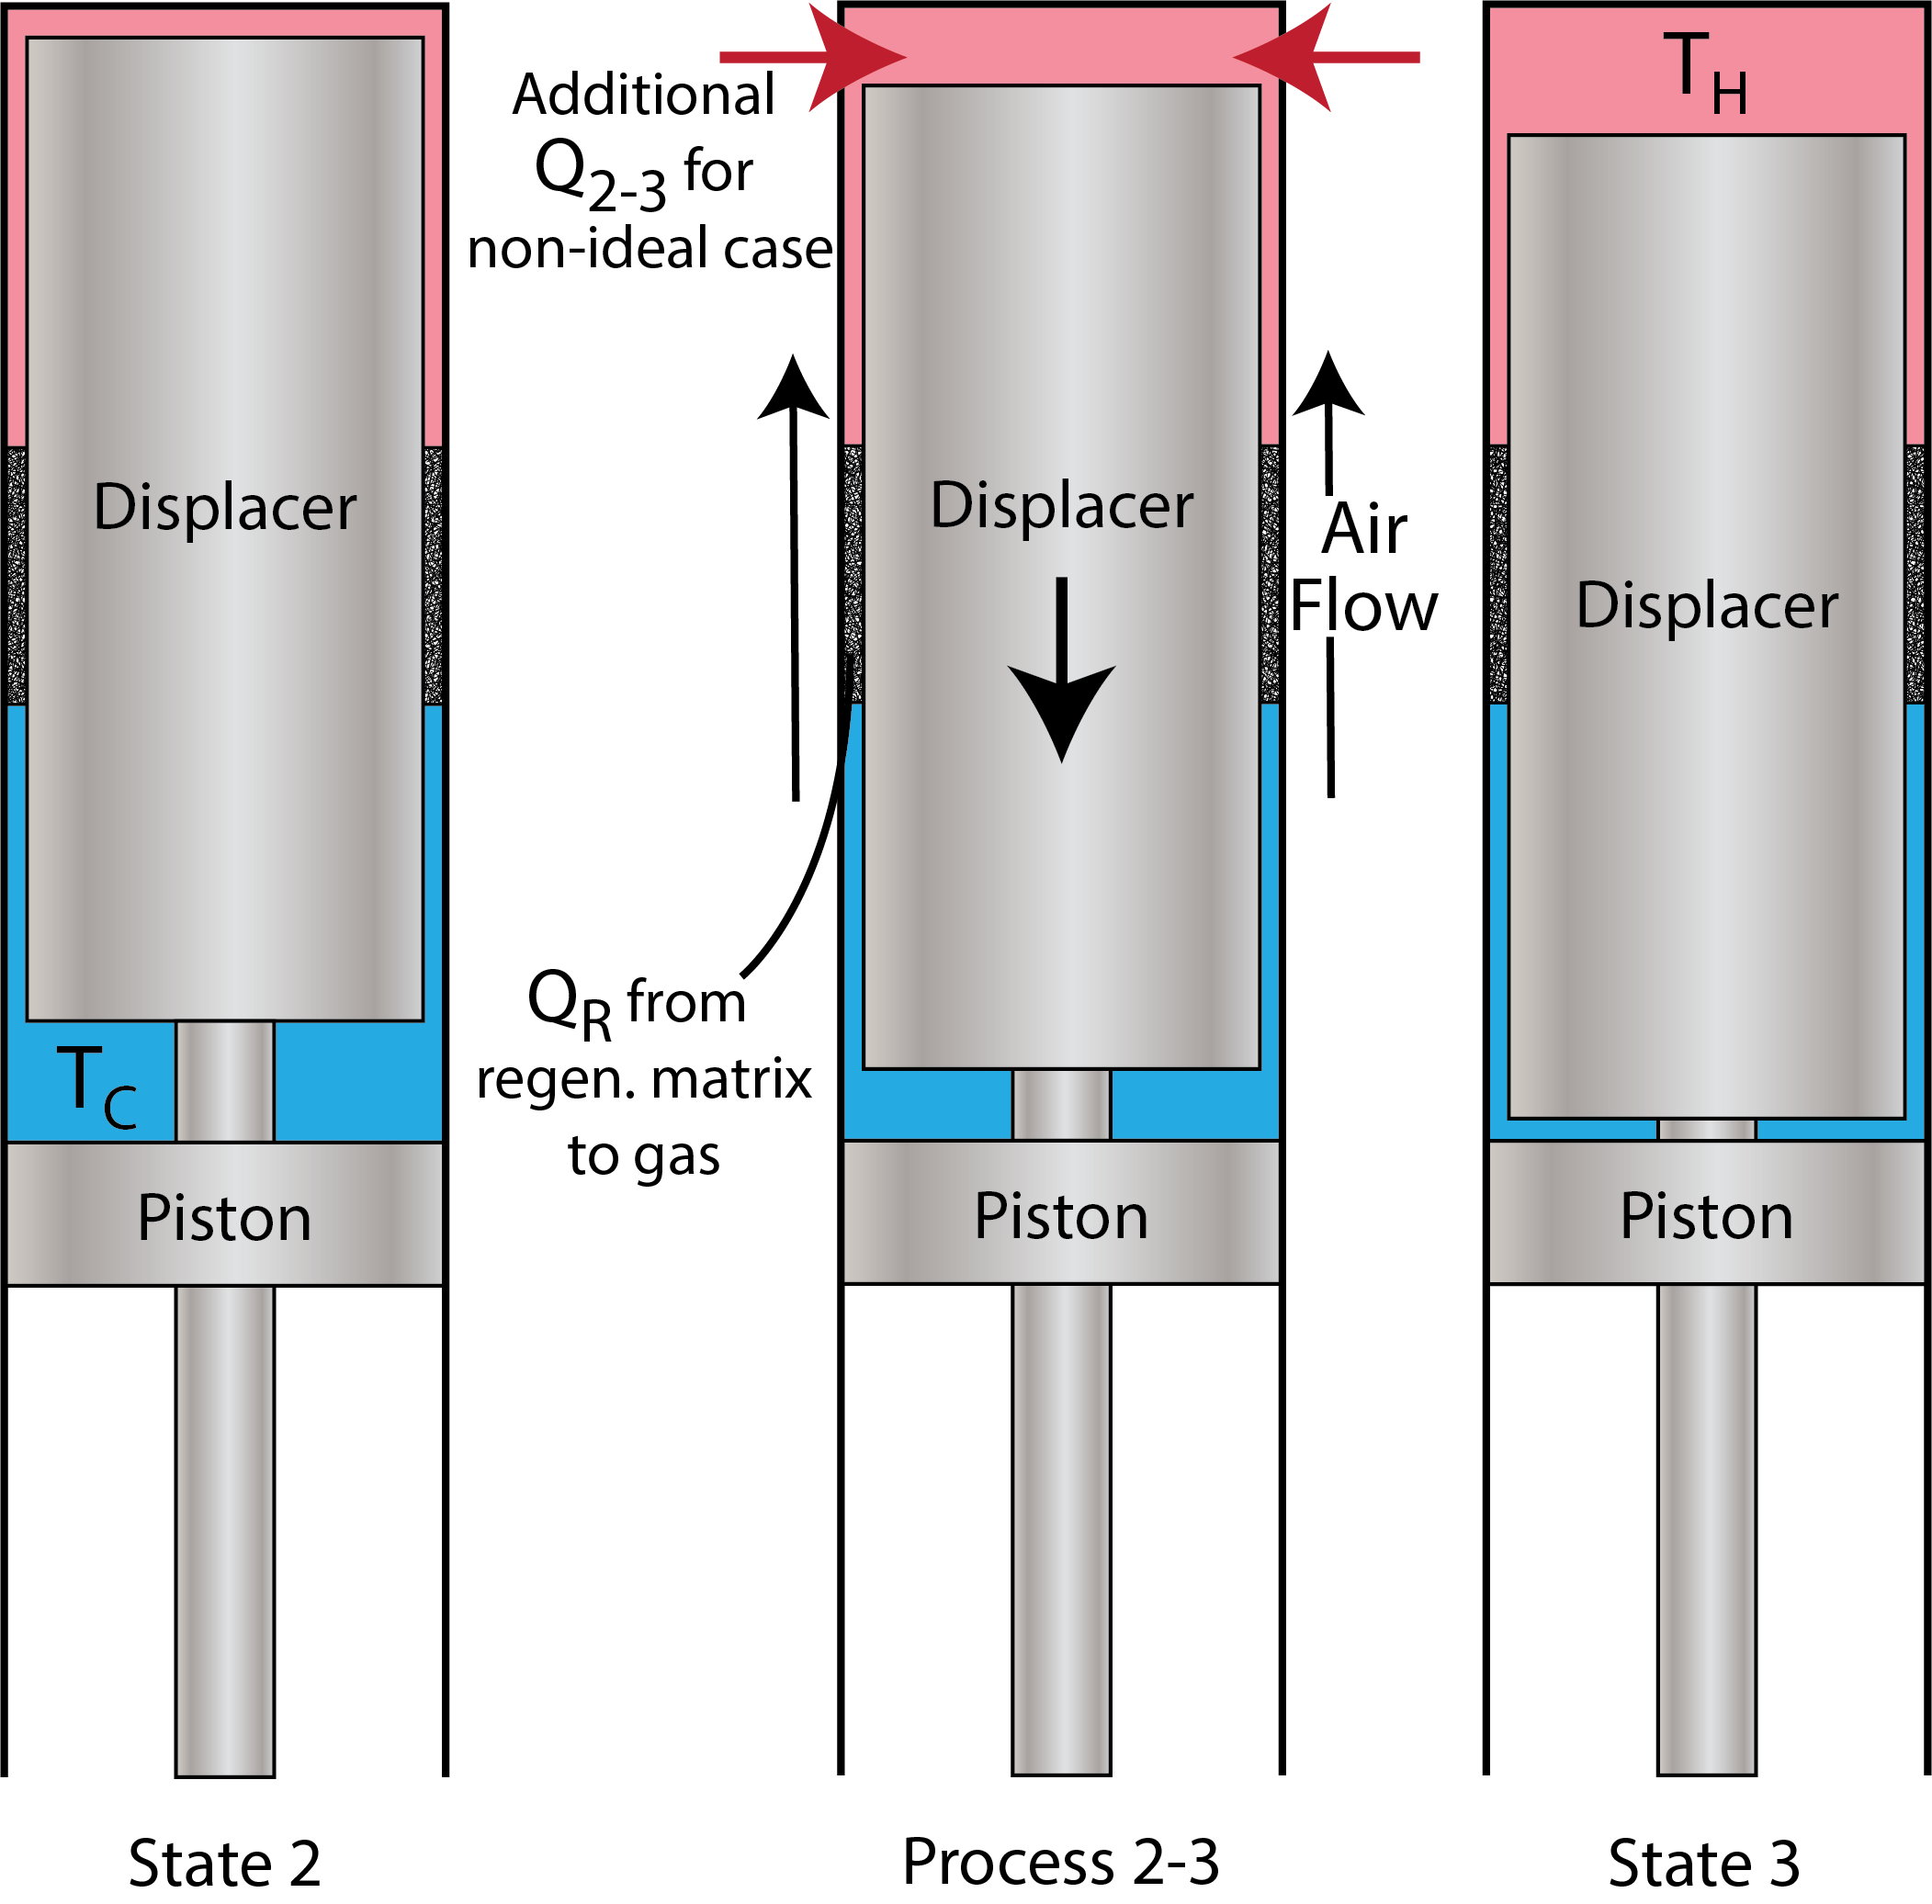
\includegraphics[width=0.6\textwidth]{StirlingEngineProcess2-3}
\caption{The heating process of the Stirling Engine.}
\label{fig:ch3_stirling23}
\end{figure}


Figure \ref{fig:ch3_stirling23} shows the movement of the displacer down into the cold region.  This in turn drives the air through the regenerator into the hot region.  The end result of this is that the air is significantly heated and ends up at $T_H$.

Importantly, there is no compression or expansion in Process 2-3.  This means no work is done between the two states, greatly simplifying our analysis:
\begin{equation} \label{eq:stirlingRegenerator}
  \Delta u_{2-3} = q_{2-3} - \cancelto{0}{w_{2-3}} \quad \rightarrow \quad q_{2-3} = c_v \left(T_H - T_C\right)
\end{equation}

% --------------------------------------------------------------------
\subsection{Process 3$\rightarrow$4 -- Isothermal Expansion}

After the air is displaced, the hot air expands, forcing back the piston.  Once again, this process is isothermal, but this time at a temperature $T_H$.

Figure \ref{fig:ch3_stirling34} shows Process 3-4, the expansion of the air at constant temperature.  The analysis mirrors that of Process 1-2.

\begin{figure}[H]
\centering
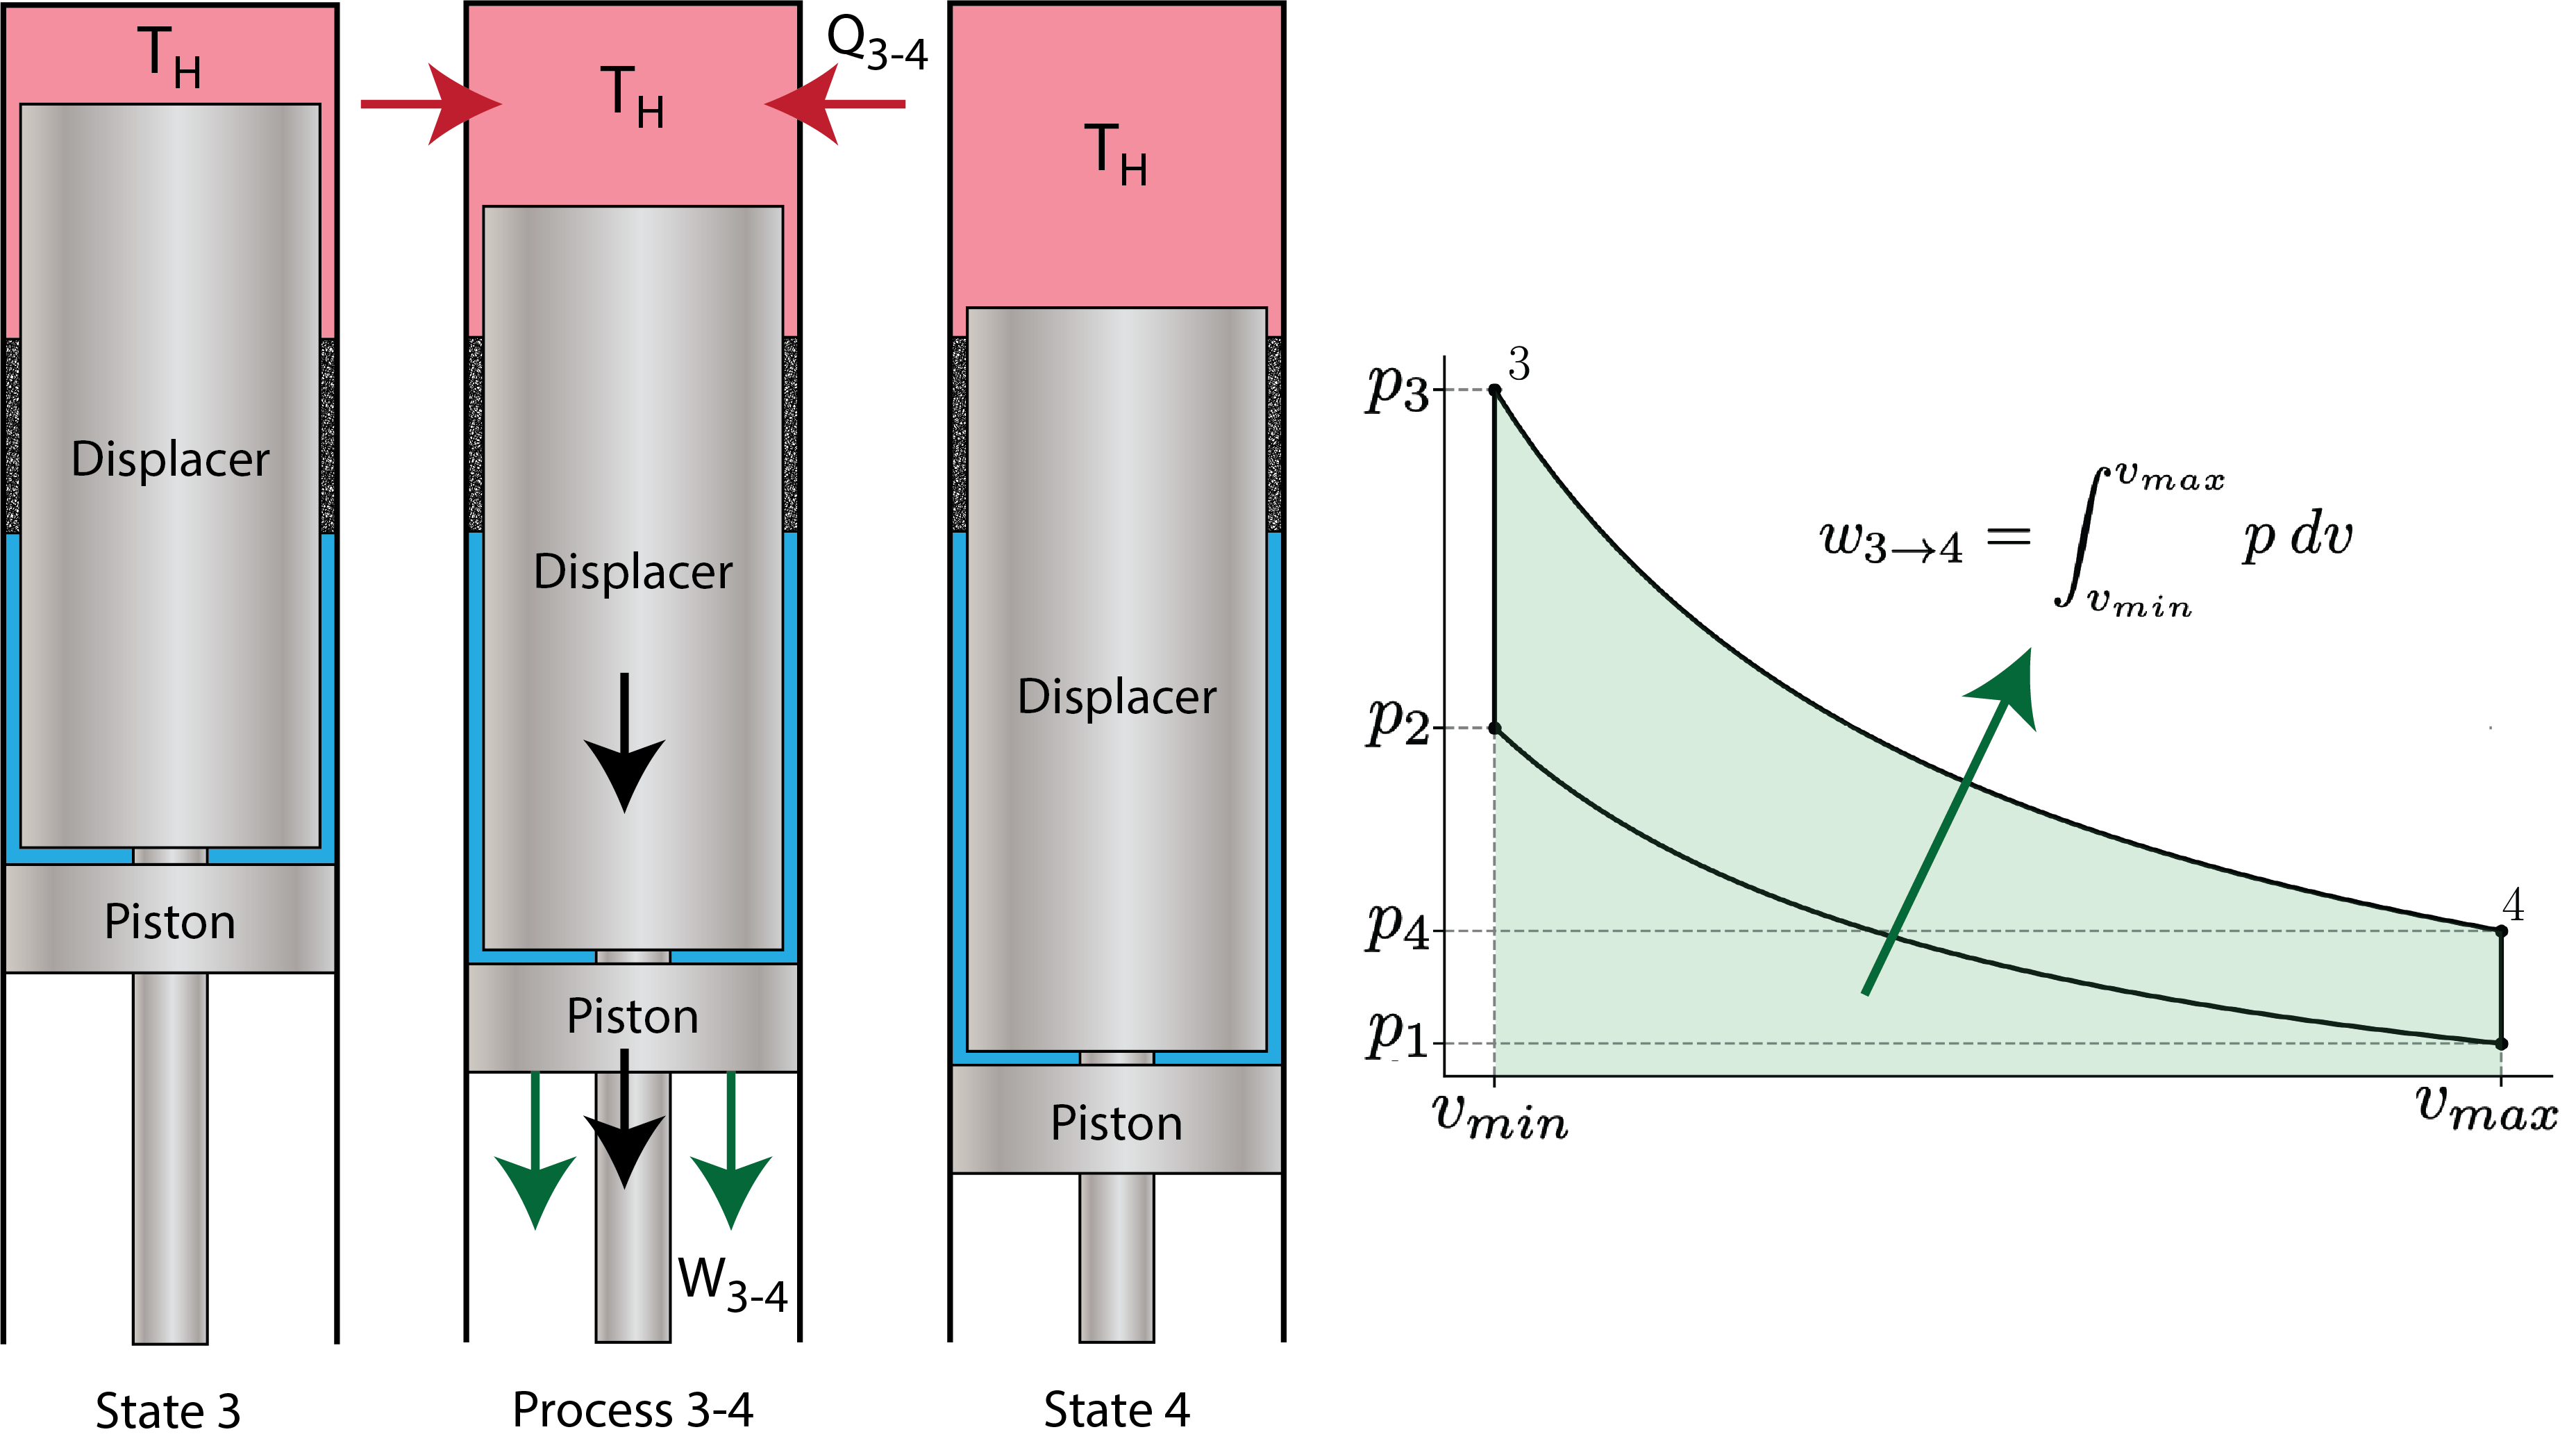
\includegraphics[width=0.9\textwidth]{StirlingEngineProcess3-4}
\caption{The expansion process of the Stirling Engine.}
\label{fig:ch3_stirling34}
\end{figure}

\begin{equation} \label{eq:stirlingExpWork}
  w_{3-4} = \int_{v_3}^{v_4} p\:dv= R T_H \int_{v_3}^{v_4} \frac{dv}{v}=RT_H\cdot  \ln\left(\frac{v_4}{v_3}\right)
\end{equation}

Fortunately, because Processes 2-3 and 4-1 are isometric (constant volume), we can make the replacements $v_3 \rightarrow v_2$ and $v_4\rightarrow v_1$ in Equation \ref{eq:stirlingExpWork}:

\begin{equation}
  w_{3-4} = RT_H \cdot \ln\left(\frac{v_1}{v_2}\right) = - \frac{T_H}{T_C} w_{1-2}
\end{equation}
\newpage
% --------------------------------------------------------------------
\subsection{Process 4$\rightarrow$1 -- Constant Volume Cooling}

Finally, Process 4-1 (shown in Figure \ref{fig:ch3_stirling41}) is essentially Process 2-3 in reverse (though with a larger volume).  The gas loses its heat to the regenerator matrix and is cooled back to $T_C$.

\begin{figure}[H]
\centering
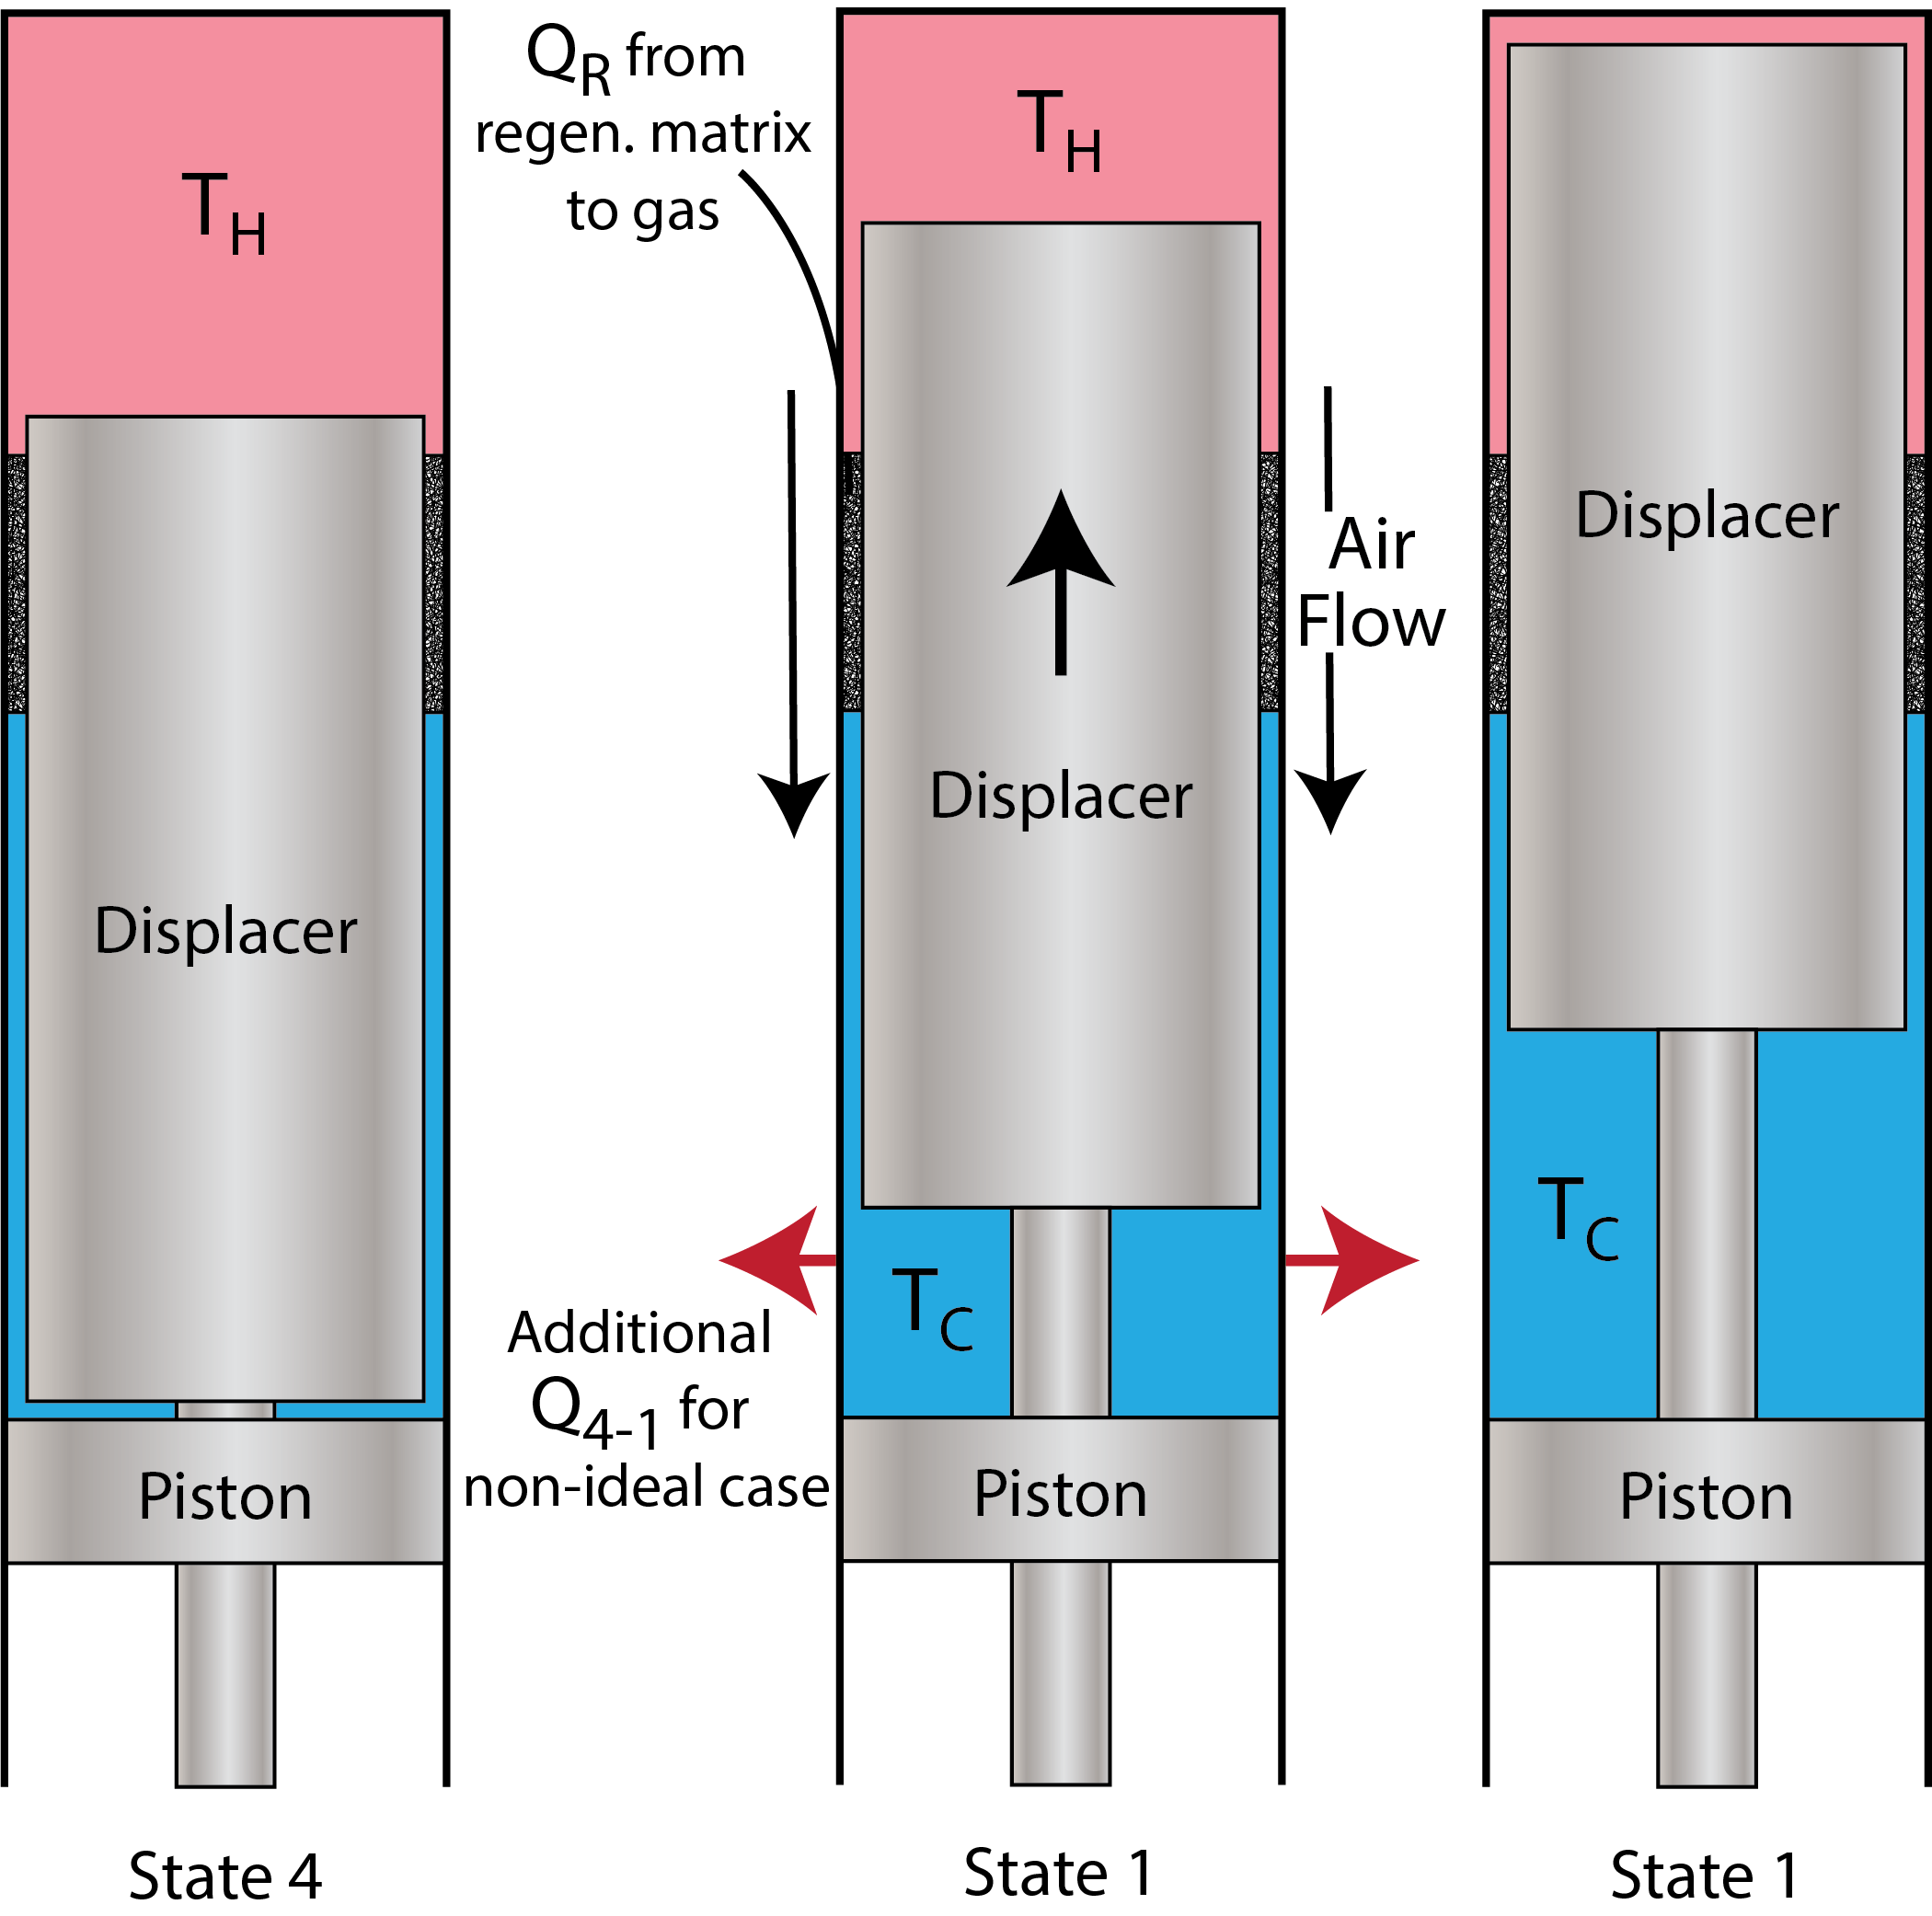
\includegraphics[width=0.6\textwidth]{StirlingEngineProcess4-1}
\caption{The cooling process of the Stirling Engine.}
\label{fig:ch3_stirling41}
\end{figure}

Again, the heat transfer is purely based on the change in temperature, as there is no work involved: $q_{4-1} = -c_v (T_H-T_C)$.  The sign is opposite of that for $q_{2-3}$ since we are cooling, rather than heating.

% --------------------------------------------------------------------
\subsection{Ideal Stirling Cycle Analysis}
For cycles, it is often helpful to write out the energy equation in tabular format, as shown in Table \ref{tab:ch3_stirling}.

\begin{table}[H]
  \centering
\def\arraystretch{1.5}
\caption{Tabular Representation of Energy Equation for Stirling Cycle}
\label{tab:ch3_stirling}
\begin{tabular}{r|ccc}
            & $\Delta u$        & $q$                                     & $w$                                    \\ \hline
Process 1-2 & 0                 & $-RT_C\cdot \ln\left(\frac{v_1}{v_2}\right)$ & $-RT_C\cdot \ln\left(\frac{v_1}{v_2}\right)$ \\
Process 2-3 & $ c_v (T_H-T_C)$ & $ c_v (T_H-T_C)$                        & 0                                      \\
Process 3-4 & 0                 &  $RT_H\cdot \ln\left(\frac{v_1}{v_2}\right)$ & $RT_H\cdot \ln\left(\frac{v_1}{v_2}\right)$ \\ 
Process 4-1 & $- c_v (T_H-T_C)$& $- c_v (T_H-T_C)$                        &  0                                    \\ \hhline{=|===}
Total (net) & 0                 & $R(T_H-T_C)\cdot \ln\left(\frac{v_1}{v_2}\right)$ & $R(T_H-T_C)\cdot \ln\left(\frac{v_1}{v_2}\right)$
\end{tabular}
\def\arraystretch{1.0}
\end{table}

We expect that $\Delta u$ for a cycle is always zero, as the cycle starts and ends at the same point.  This implies in turn that $q_{net} = w_{net}$, which is exactly what we see in Table \ref{tab:ch3_stirling}.  In fact, the purpose of the Stirling engine is to turn the net heat transfer into work.  The heat transfer to and from the regenerator doesn't come into play, as the heat transfer in Process 2-3 perfectly cancels with the heat transfer in Process 4-1.  The total work done (and the total heat added to the system) can be simplified to:

\begin{equation} \label{eq:ch3_netWorkStirling}
  q_{net} = w_{net} = R\Delta T\cdot \ln (r)
\end{equation}

where $\Delta T$ is the difference between the hot and cold temperatures and $r$ is the {\bf compression ratio}, defined as:
\begin{equation}\label{eq:ch3_compressionRatio}
  r = \frac{v_{\rm max}}{v_{\rm min}}=\frac{V_{\rm max}}{V_{\rm min}}
\end{equation}
We can also define the {\bf thermal efficiency} as the ratio between the input heat and the net work.  This efficiency is a picture of how much work we can get out of an engine based on the amount of fuel we burn.
\begin{align} \label{eq:ch3_StirlingEfficiency}
  \nonumber \eta_{th} &= \frac{w_{net}}{q_{in}} = \frac{w_{net}}{q_{3-4}} = \frac{R\Delta T\cdot \ln (r)}{RT_H\cdot \ln(r)} \\
  \eta_{th} &= \frac{\Delta T}{T_H} = 1 - \frac{T_C}{T_H}
\end{align}

Equation \ref{eq:ch3_StirlingEfficiency} is the maximum theoretical efficiency achievable from a heat engine, and is typically referred to as the {\bf Carnot efficiency}.

% --------------------------------------------------------------------
\subsection{Stirling Engines without Regeneration}
Note that the ideal case assumes that the regenerator is able to fully heat/cool the air in Processes 2-3 and 4-1.  If this is not the case (or if there is no regenerator present), then the extra heat $Q_{2-3}$ must be provided by the heater, which will reduce the efficiency.  In the case of no regenerator, the efficiency becomes:
\begin{equation} \label{eq:ch3_StirlingEfficiencyNoRegen}
  \nonumber \eta_{th} = \frac{w_{net}}{q_{in} + q_{2-3}} = \frac{R\Delta T\cdot \ln (r)}{(RT_H\cdot \ln(r)+c_v\Delta T)}
\end{equation}

This is a little difficult to draw conclusions from, but let's look at a sample case with air as the working fluid ($c_v \approx 2.5 R$), $T_C = 300\ {\rm K}$, $T_H = 600\ {\rm K}$, and $r = 1.3$.  That gives us an ideal thermal efficiency of $\eta_{th, {\rm regen}} = 0.5$ with the regenerator, and an ideal thermal efficiency of $\eta_{th, {\rm no\ regen}} = 0.097$!  Having a regenerator is hugely important!

Another important note is that even with a regenerator, the practical Stirling cycle has many losses associated with it and does not really involve isothermal processes, nor ideal regeneration. Furthermore, Stirling cycle machines do not typically start and stop the pistons perfectly, meaning that the $p$-$V$ diagram has a more oval shape, rather than the sharp edges defined in the above diagrams. Nevertheless we use the ideal Stirling cycle to get an initial understanding and appreciation of the cycle performance.
\newpage
\begin{example}{Stirling Cycle Engine/Generator} 
  This exercise concerns the ideal performance of the \href{https://www.microgen-engine.com/engines/}{Microgen 1050 Watt engine} which is gas fired and was designed to generate electricity (1kWe) as well as to provide hot water for a private home. This engine has a similar configuration to the Stirling engine discussed in Section \ref{sec:idealStirling}.  (Note that the values presented here are not actual values of the Microgen Engine, however were devised by your instructor for purposes of this exercise only).

  The working fluid is helium, which has an gas constant $R$ = 2.077 kJ/kg K, and constant volume specific heat $c_v$ = 3.116 kJ/kg K. (refer: Ideal Gas Properties).  State (1) is defined at a maximum volume of 650 $\rm cm^3$ and a pressure of 10 bar, and State (2) is defined at a minimum volume of 550 $\rm cm^3$.  Process 1-2 is isothermal compression at $T_C$ = 50°C, Process 2-3 is isometric heating, using a regenerator to source the heat.  Process 3-4 is isothermal expansion at $T_H$ = 500°C, and Process 4-1 is isometric cooling, again using the regenerator as a heat sink.
  \begin{enumerate}[a)]
  \item From the given conditions at state 1 determine the mass of working gas (helium) used in the cycle.
    
  \item Determine the net work done per cycle (kiloJoules): $W_{exp}$ + $W_{comp}$ (Note that the compression work $W_{comp}$ is always negative). At a frequency of 50 Hertz (cycles per second) determine the power output produced by the engine.
    
  \item Determine the heat absorbed in the expansion space $Q_{in}$ during the expansion process (3)-(4).
    
  \item Evaluate the Thermal Efficiency $\eta_{th}$, defined as: $\eta_{th} = (W_{exp} + W_{comp}) / Q_{in}$. (Net mechanical work done divided by the heat supplied externally by the gas burner).
    
  \item Determine the amount of thermal power rejected to the cooling water. Note that at a temperature of 50°C this is suitable for providing hot water for the home, as well as providing home space heating capability.
    
  \item Determine the amount of heat transferred to the working fluid $Q_R$ as it passes through the regenerator during process (2)-(3). If this heat were to be supplied externally by the gas burner, (i.e. no regenerator) what would be the new value of thermal efficiency $\eta_{th}$? 
  \end{enumerate}
  
  {\bf Solution Approach}
  \begin{enumerate}[a)]
  \item  We can find the mass through the ideal gas law, letting 1 $\rm cm^3$ = $1\times 10^{-6}m^3$:
    \begin{align*}
      p_1v_1=RT_1 \quad\quad \rightarrow & \quad\quad v_1 = \frac{RT_1}{p_1} \\
      & \quad\quad v_1 = \frac{2.077 {\rm\ kJ/kgK} \cdot 323.15{\rm\ K}}{1000\ \rm kPa} \\
      & \quad\quad \redbox{v_1 = 0.6712 \rm\ m^3/kg} \\
      v_1 = \frac{V_1}{m} \quad\quad \rightarrow & \quad\quad \redbox{m = \frac{6.5\times 10^{-4} \rm\ m^3}{0.6712\ \rm m^3/kg} = 9.68\times 10^{-4}\ \rm kg}
    \end{align*}
  \item The net work comes from Equation \ref{eq:ch3_netWorkStirling}:
    \begin{align*}
      W_{net} &= m R \left(T_H-T_C\right) \ln{\left(\frac{V_1}{V_2}\right)} \\
      W_{net} &= ({0.968\ \rm g}) \left(2.077\frac{\rm kJ}{\rm kg K}\right) (450\ {\rm K}) \ln{\left(\frac{650\ \rm cm^3}{550\ \rm cm^3}\right)} \quad\rightarrow\quad \redbox{W_{net} = 0.151\ \rm kJ}
    \end{align*}
    We can convert from work to power by multiplying by the frequency (units of Hz are the same as 1/s):
    \begin{equation*}
      \dot{W}_{net} = W_{net} \cdot f = {0.151\ \rm kJ} \cdot 50 \frac{1}{\rm s} \quad\rightarrow\quad \redbox{\dot{W}_{net} = 7.55\rm\ kW}
    \end{equation*}
  \item The heat absorbed in the expansion space can be calculated from Equation \ref{eq:stirlingExpWork}, recognizing that the constant-temperature process results in no change in internal energy:
    \begin{align*}
      W_{exp} &= Q_{exp} = m R T_H \ln{\left(\frac{V_4}{V_3}\right)} \\
      Q_{exp} &= ({0.968\ \rm g}) \left(2.077\frac{\rm kJ}{\rm kg K}\right) (773.15\ {\rm K}) \ln{\left(\frac{650\ \rm cm^3}{550\ \rm cm^3}\right)} \ \rightarrow\ \redbox{Q_{exp} = 0.260\ \rm kJ}
    \end{align*}
    This is equivalent to $\redbox{\dot{Q}_{exp} = 13.0\rm\ kJ}$.
  \item We can find the thermal efficiency from the results of the previous two parts:
    \begin{equation*}
      \eta_{th} = \frac{W_{net}}{Q_{in}} = \frac{0.151\rm\ kJ}{0.260\rm\ kJ} \quad\rightarrow\quad \redbox{\eta_{\th} = 58\%}
    \end{equation*}
  \item The heat rejected to the cooling water can be calculated directly as in part c), or by recognizing that $Q_{in} - Q_{out} = W_{net}$.
    \begin{equation*}
      Q_{out} = Q_{in} - W_{net} = 0.260{\rm\ kJ} - 0.151{\rm\ kJ} \quad\rightarrow\quad \redbox{Q_{out} = 0.109{\rm\ kJ}}
    \end{equation*}
  \item The regenerator transfers enough heat to change the temperature of the helium from 50°C to 500°C.  This heat can be calculated through the definition of the $c_v$, as in Equation \ref{eq:stirlingRegenerator}:
    \begin{equation*}
      Q_R = m c_v \Delta T = ({0.968\ \rm g})\left(3.116\frac{\rm kJ}{\rm kg K}\right) (450\ {\rm K}) \quad\rightarrow\quad \redbox{Q_R = 1.36\rm\ kJ}
    \end{equation*}
    Adding the regenerator heat transfer to the heat supplied to the gas burner allows us to find the new thermal efficiency:
    \begin{equation*}
      \eta_{th} = \frac{W_{net}}{Q_{in}+Q_R} = \frac{0.151\rm\ kJ}{0.260\rm\ kJ + 1.35\rm\ kJ} \quad\rightarrow\quad \redbox{\eta_{th} = 9.3\%}
    \end{equation*}
    This value is in line with the efficiency calculated in the previous section.
  \end{enumerate}
  
\end{example}

% --------------------------------------------------------------------
\section{Stirling Cycle Cooling} \label{sec:ch3_StirlingCooling}
% --------------------------------------------------------------------

One important aspect of Stirling cycle machines that we need to consider is that the cycle can be reversed - if we put net work into the cycle then it can be used to pump heat from a low temperature source to a high temperature sink.  This results in a very compact refrigerator, which can reach very low temperatures.  This technology has been used in a few specific instances, primarily in \href{https://www.stirlingultracold.com}{ultra-low-temperature freezers for biomedical uses}.  The cycle used in standard air conditioning units is discussed in Section \ref{sec:Refrigeration}.

\begin{figure}[H]
\centering
\scalebox{1}[-1]{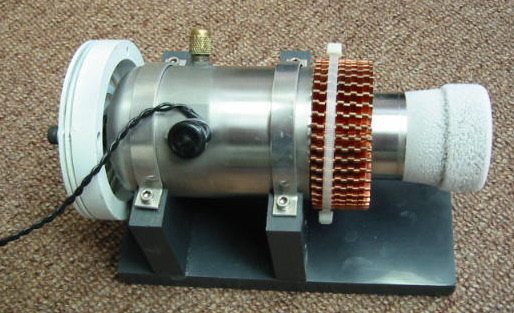
\includegraphics[angle=180, width=0.75\textwidth]{StirlingCooler}}
\caption{The M100B Stirling Cooler from Global Cooling (now Stirling Ultracold).}
\label{fig:ch3_stirlingCooler}
\end{figure}

Figure \ref{fig:ch3_stirlingCooler} shows an example of a Stirling Cooler.  Power is provided through the small electrical cord, while ice crystals can be seen forming on the left-hand side of the cooler.  Refer to the schematic in Figure \ref{fig:ch3_M100BSchematic} to identify the various parts of the cooler.

\begin{figure}[H]
\centering
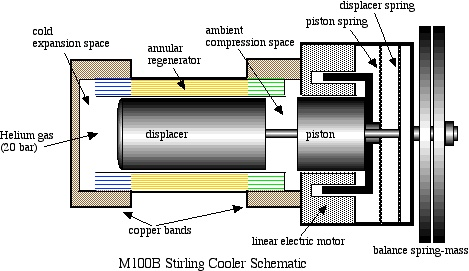
\includegraphics[width=0.75\textwidth]{M100Bschem}
\caption{Schematic of M100B Stirling Cooler from Global Cooling.}
\label{fig:ch3_M100BSchematic}
\end{figure}

%Conceptually the cooler is an extremely simple device, consisting essentially of only two moving parts - a piston and a displacer. The displacer shuttles the working gas (helium) between the compression and expansion spaces. The phasing between the piston and displacer is such that when the most of the gas is in the ambient compression space then the piston compresses the gas while rejecting heat to the ambient. The displacer then displaces the gas through the regenerator to the cold expansion space, and then both displacer and piston allow the gas to expand in this space while absorbing heat at a low temperature.

Figure \ref{fig:ch3_StirlingCoolingCycle} shows the cycle used by the Stirling Cooler.  Heat is rejected to the environment ($Q_H$) in Process 1-2, rejected to the regenerator ($Q_R$) in Process 2-3, absorbed from the refrigerated space ($Q_C$) in Process 3-4, and finally absorbed from the regenerator ($Q_R$) in Process 4-1. More work is required to drive Process 1-2 than is regained in Process 3-4, meaning that the net work for this cycle is negative.  In other words, work is required to move heat from the cold side to the hot side.

\begin{figure}[H]
\centering
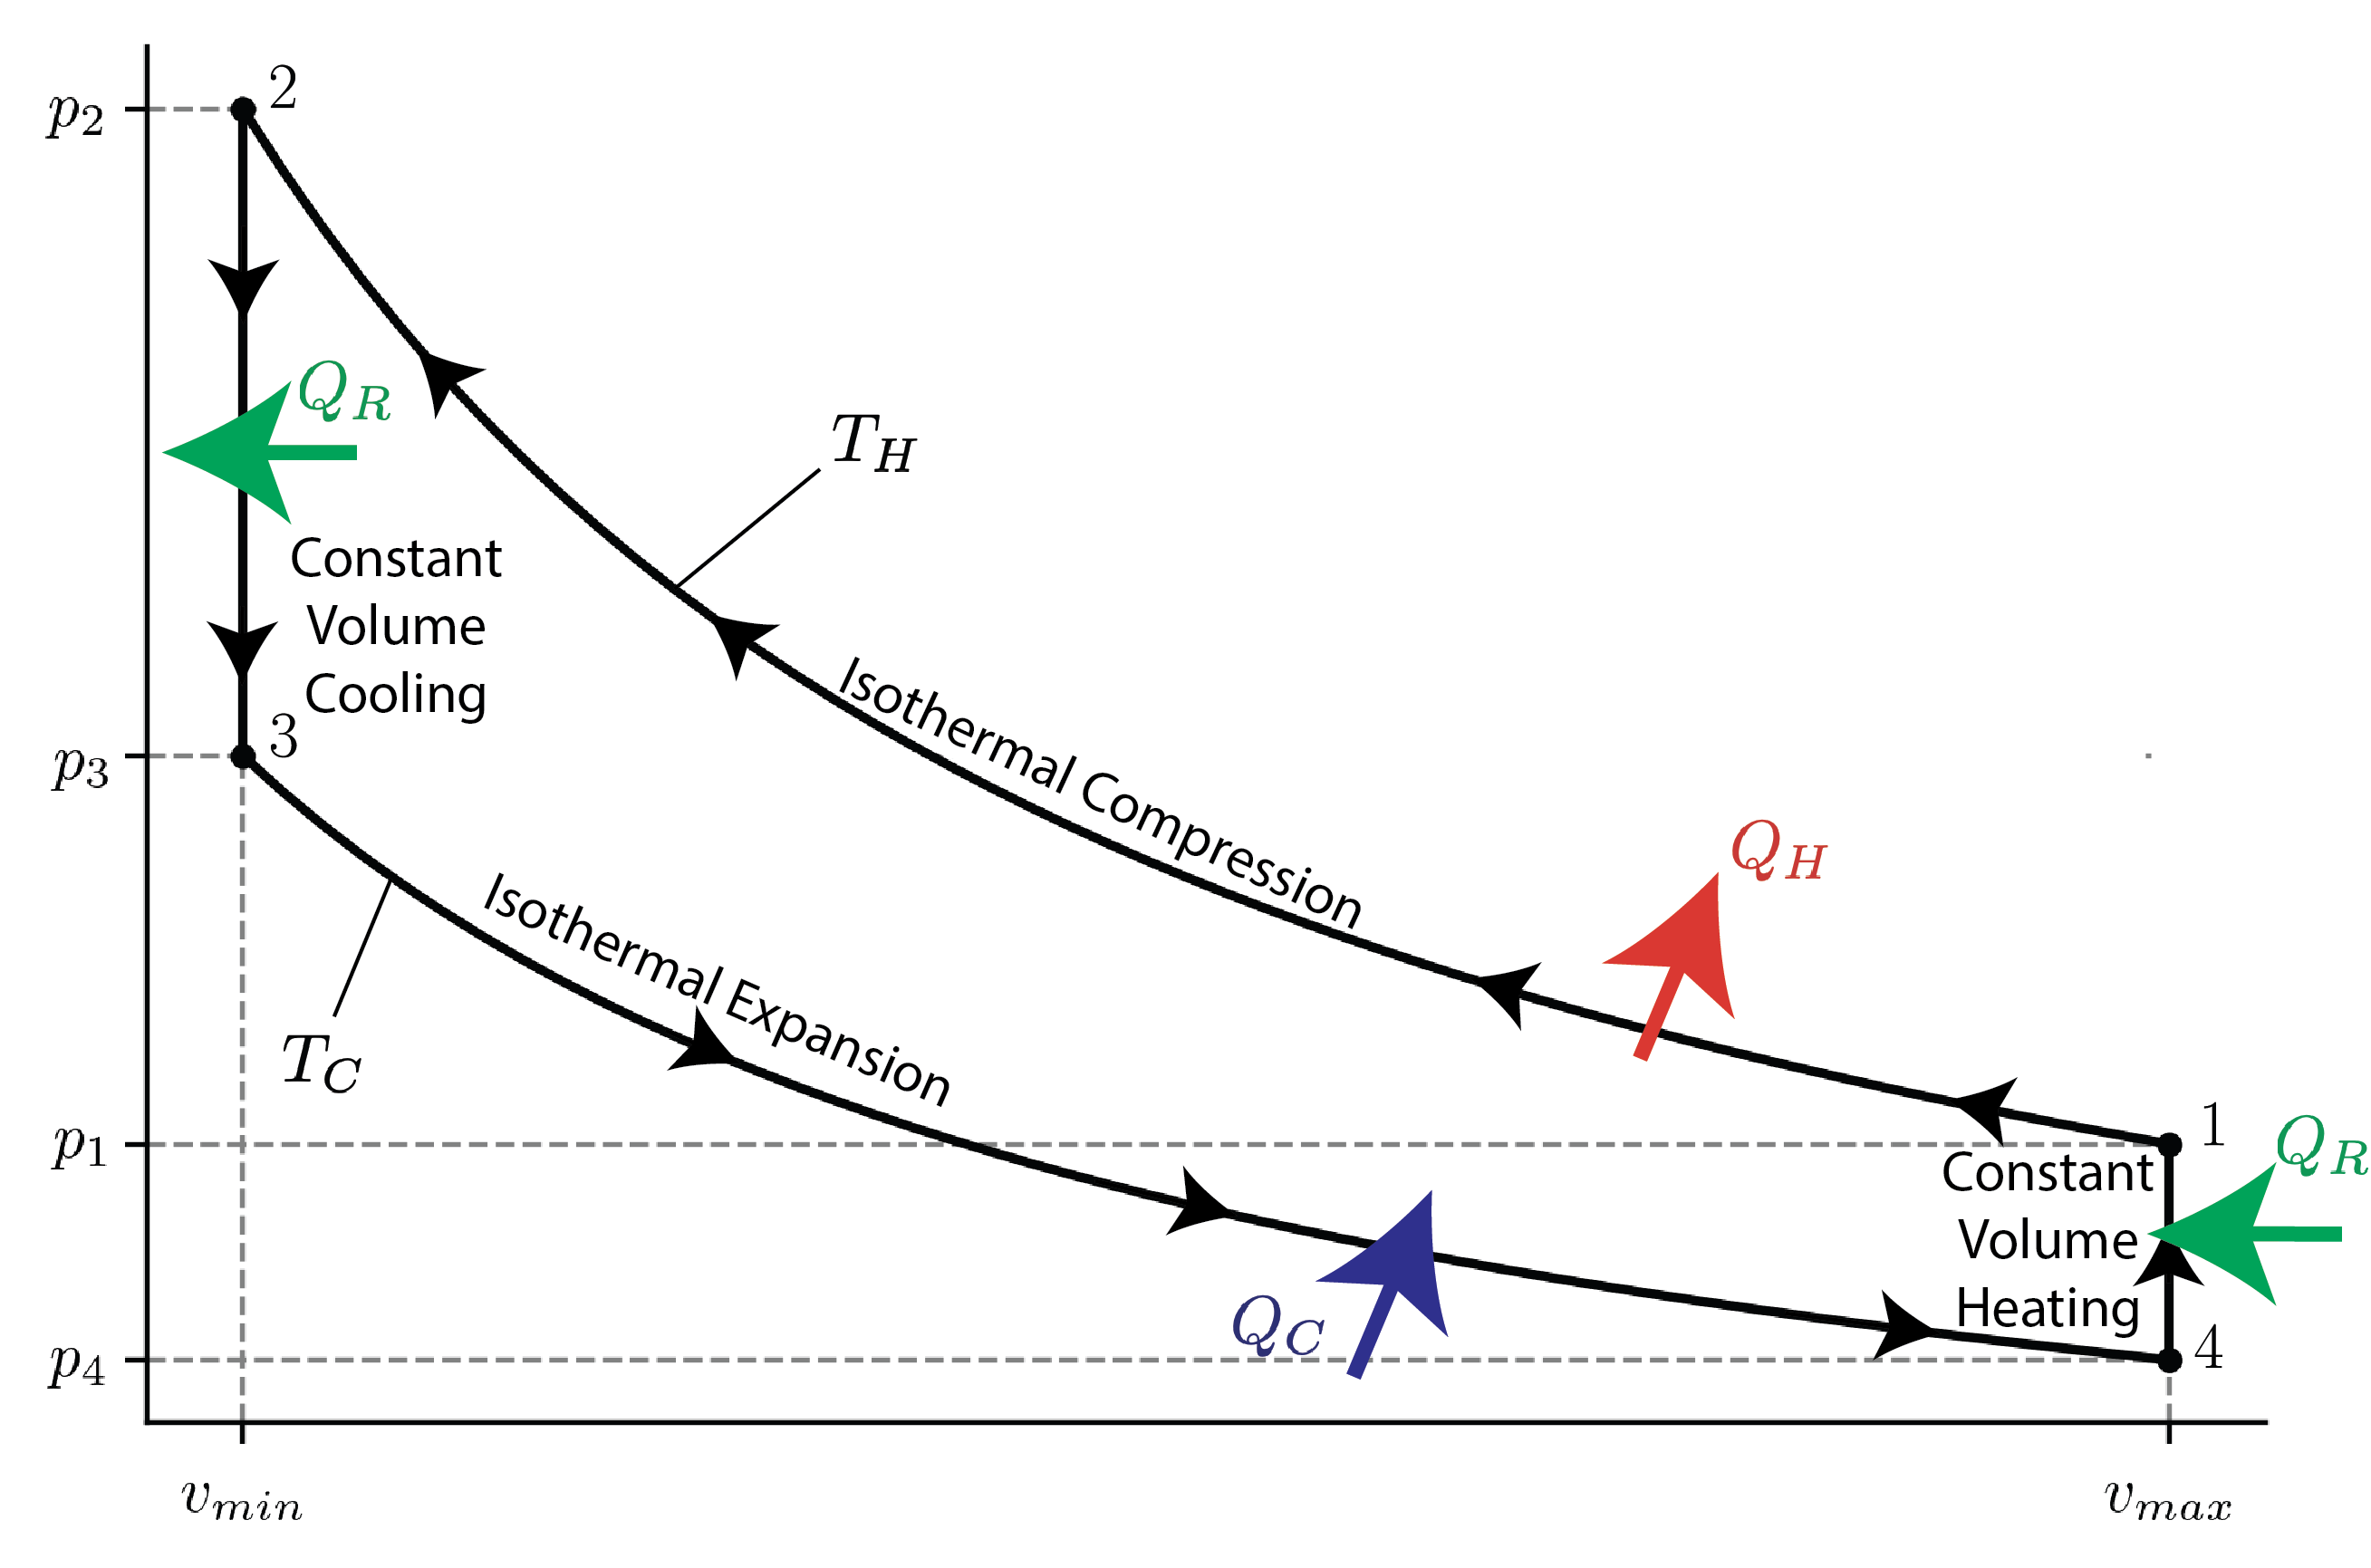
\includegraphics[width=0.75\textwidth]{StirlingCoolingDiagram}
\caption{$p$-$v$ diagram of the Stirling Cooling Cycle.}
\label{fig:ch3_StirlingCoolingCycle}
\end{figure}

Cooling cycles do not use the thermal efficiency as an indicator of performance.  Following the general idea that ``efficiency'' is ``what we get out''/''what we put in'', the efficiency of a cooling cycle is defined at the Coefficient of Performance for a refrigeration cycle, $COP_R$:
\begin{equation*}
  COP_R = \frac{q_{in}}{w_{net}}
\end{equation*}

The heat absorbed, $q_{in}$, is the benefit we get from the cooling cycle, as we are seeking to remove heat from a refrigerated space.  The net work, $w_{net}$, is what we have to pay to get that benefit, as we are doing work on the cycle.

Conversely, if we chose to think of this cycle as a way to add heat to a heated space, we would arrive at the Coefficient of Performance for a heat pump cycle, $COP_{HP}$:
\begin{equation*}
  COP_{HP} = \frac{q_{out}}{w_{net}}
\end{equation*}

In this case, the heat rejected to the heated space is the benefit from the cycle, which leads to a change in our ``efficiency'' calculations.

Example \ref{ex:StirlingCooling} investigates the Stirling cooling cycle in more detail.
\newpage
\begin{example}[label={ex:StirlingCooling}]{Stirling Cycle Cooling}

  A Stirling cooling cycle is defined as follows:
  \begin{itemize}
  \item Compression occurs at a constant temperature of $T_H$ = 30°C.
  \item Expansion occurs at a constant temperature of $T_C$ = -20°C.
  \item The maximum volume is 35 $\rm cm^3$
  \item The minimum volume is 30 $\rm cm^3$
  \item The pressure immediately before compression is 1.9 MPa.
  \item The working fluid is helium, which has an gas constant $R$ = 2.077 kJ/kg K, and constant volume specific heat $C_v$ = 3.116 kJ/kg K.
  \end{itemize}

\begin{enumerate}[a)]
\item Determine the heat absorbed in the expansion stroke (Joules). Determine also the heat power absorbed (Watts). Note that the cycle frequency is the line frequency (f = 60 Hz).

\item Determine the net work done per cycle (Joules): $W_{net} = W_{comp} + W_{exp}$ (Note that the compression work $W_{comp}$ is always negative). Determine also the power supplied to the linear electric motor (Watts).
  
\item Evaluate the Coefficient of Performance of the refrigerator defined as: $COP_R = Q_C / W_{net}$. (heat absorbed in the expansion space divided by the net work done). 

\item Determine the amount of heat rejected by the working fluid $Q_R$ as it passes through the regenerator matrix during constant volume cooling.

\item If there were no regenerator present then this heat would need to be removed from the gas by the expansion process in order to reduce the temperature to the cold temperature of the freezer. How would this affect the performance of the cooler? Discuss the importance of an effective regenerator in the Stirling cycle cooler.
\end{enumerate}

{\bf Solution Approach}

First off, let's find the mass of the working fluid.

For the first state, pressure and temperature are both defined, as is the total volume.  This is sufficient for us to find the mass of the working fluid.  As part of the process, we need to convert 35 $\rm cm^3$ to $3.5\times 10^{-5} \rm m^3$.
\begin{align*}
  p_1v_1=RT_1 \quad\quad \rightarrow & \quad\quad v_1 = \frac{RT_1}{p_1} \\
  & \quad\quad v_1 = \frac{2.077 {\rm\ kJ/kgK} \cdot 303.15{\rm\ K}}{1900\ \rm kPa} \\
  & \quad\quad \redbox{v_1 = 0.3314 \rm\ m^3/kg} \\
  v_1 = \frac{V_1}{m} \quad\quad \rightarrow & \quad\quad \redbox{m = \frac{3.5\times 10^{-5} \rm\ m^3}{0.3314\ \rm m^3/kg} = 1.056\times 10^{-4}\ \rm kg}
\end{align*}

\begin{enumerate}[a)]
\item Once we have the mass, we can use Table \ref{tab:ch3_stirling} for the analysis, except we need to replace $T_C$ with $T_H$ and vice-versa. The heat transfer is therefore:
  \begin{align*}
    Q_{exp} &= m R T_C \ln{\left(\frac{v_4}{v_3}\right)} = m R T_C \ln{\left(\frac{V_4}{V_3}\right)} \\
    Q_{exp} &= ({0.1056\ \rm g}) \left(2.077\frac{\rm kJ}{\rm kg K}\right) (253.15\ {\rm K}) \ln{\left(\frac{35\ \rm cm^3}{30\ \rm cm^3}\right)} \quad\rightarrow\quad \redbox{Q = 8.56\ \rm J}
  \end{align*}

  We can get to heat power absorbed simply by multiplying by the frequency of 60 Hz.
  \begin{equation*}
    \dot{Q}_{exp} = Q \cdot f = {8.56\ \rm J} \cdot 60 \frac{1}{\rm s} \quad\rightarrow\quad \redbox{\dot{Q}_{exp} = 513.6\rm\ W}
  \end{equation*}

\item The net work can be obtained from Equation \ref{eq:ch3_netWorkStirling}, again with $T_C$ and $T_H$ switched.
  \begin{align*}
    W_{net} &= m R \left(T_C-T_H\right) \ln{\left(\frac{V_1}{V_2}\right)} \\
    W_{net} &= ({0.1056\ \rm g}) \left(2.077\frac{\rm kJ}{\rm kg K}\right) (50\ {\rm K}) \ln{\left(\frac{35\ \rm cm^3}{30\ \rm cm^3}\right)} \quad\rightarrow\quad \redbox{W_{net} = -1.69\ \rm J}
  \end{align*}
  Note that the work done is negative, indicating that work is performed on the cycle, rather than provided by it.

  We can again find the power by multiplying by $f$.  This becomes $\redbox{\dot{W}_{net} = -101\rm\ W}$.
\item The Coefficient of Performance is easily determined from the two previous results.
  \begin{equation*}
    COP_R = \frac{Q_C}{W_{net}} = \frac{8.56\ \rm J}{1.69\ \rm J} \quad\rightarrow\quad \redbox{COP_R = 5.07}
  \end{equation*}

\item The heat absorbed/rejected by the regeneration matrix can be found from Equation \ref{eq:stirlingRegenerator}.
  \begin{equation*}
    Q_R = m c_v \Delta T = ({0.1056\ \rm g})\left(3.116\frac{\rm kJ}{\rm kg K}\right) (50\ {\rm K}) \quad\rightarrow\quad \redbox{Q_R = 16.45 J}
  \end{equation*}
  This equates to $\redbox{\dot{Q}_{R} = 988\rm\ W}$.
\item Without regeneration, we would expect a drastically lower $COP_R$ value.  It's difficult to see exactly how this comes about, as there is no easy mechanism through which we can compensate for the lack of a regenerator (like we simply added more heat in the Stirling engine).
\end{enumerate}


\end{example}

%% The process between state 1 and 2 is isothermal compression, meaning that $T_2 = T_1$, and $V_2$ is given as 35 $\rm cm^3$.  We can calculate the new pressure using the ideal gas law.  While we could plug in all the values directly, I prefer to create a ratio of the two ideal gas law equations, as follows:
%% \begin{align*}
%%   \frac{p_2}{p_1}\frac{v_2}{v_1} &= \cancel{\frac{R}{R}}\cancel{\frac{T_2}{T_1}} = 1 \\
%%   p_2 &= p_1 \frac{v_1}{v_2} \\
%%   p_2 &= 1.9 {\rm\ MPa} \cdot \frac{35 \rm\ cm^3}{30 \rm\ cm^3} \quad \rightarrow \quad \redbox{p_2 = 2.217\rm\ MPa}
%% \end{align*}
%% Process 2-3 is constant volume cooling to $T_3$ = -20°C.  We can again find the new pressure using the ratio of ideal gas law equations:
%% \begin{align*}
%%   \frac{p_3}{p_2}\cancel{\frac{v_3}{v_2}} &= \cancel{\frac{R}{R}}\frac{T_3}{T_2} = 1 \\
%%   p_3 &= p_2 \frac{T_3}{T_2} \\
%%   p_3 &= 2.217 {\rm\ MPa} \cdot \frac{253.15 \rm\ K}{303.15 \rm\ K} \quad \rightarrow \quad \redbox{p_3 = 1.851\rm\ MPa}
%% Process 3-4 is constant temperature expansion back to $V_4=V_1=35\rm\ cm^3$.  We can find $p_4$ the same way as before:
%% \begin{align*}
%%   \frac{p_4}{p_3}\frac{v_4}{v_3} &= \cancel{\frac{R}{R}}\cancel{\frac{T_4}{T_3}} = 1 \\
%%   p_4 &= p_3 \frac{v_3}{v_4} \\
%%   p_4 &= 1.851 {\rm\ MPa} \cdot \frac{30 \rm\ cm^3}{35 \rm\ cm^3} \quad \rightarrow \quad \redbox{p_4 = 1.586\rm\ MPa}
%% \end{align*}



% --------------------------------------------------------------------
\section{Ideal Gas Adiabatic Processes} \label{sec:ch3_idealGasAdiabatic}
The next two cycles both rely heavily on {\bf adiabatic} processes.  In order to discuss those cycles, we will look closer at adiabatic processes for an ideal gas.

Adiabatic processes are simply processes without heat transfer.  This means that the change in internal energy is purely due to the work done.

\begin{equation*}
  \cancelto{0}{\delta q} - \delta w = du
\end{equation*}

Substituting $\delta w = p\: dV$ and $du = c_v dT$ gives us:
\begin{equation*}
  -p dv = c_v dT
\end{equation*}

With $pv = RT$, we calculate:

\begin{equation*}
  -\frac{RT}{v} dv = c_v dT \quad \rightarrow \quad c_v dT + \frac{RT}{v} dv =0 \quad \rightarrow \quad c_v \frac{dT}{T} + R \frac{dv}{v} = 0
\end{equation*}

Now we integrate:

\begin{align*}
  \int_1^2 \left(c_v \frac{dT}{T} + R \frac{dv}{v}\right) &= 0\\
  \int_{T_1}^{T_2} c_v \frac{dT}{T} + \int_{v_1}^{v_2} R \frac{dv}{v} &= 0 \\
  c_v \ln \frac{T_2}{T_1} + R \ln \frac{v_2}{v_1} &= 0
\end{align*}

Rearranging slightly gives us:

\begin{equation} \label{eq:ch3_adiabaticTv}
  \ln \frac{T_2}{T_1} = -\frac{R}{c_v} \ln \frac{v_2}{v_1}
\end{equation}

Remembering that $e^{c \ln x} = x^c$, we can arrive at:

\begin{equation*}
  \frac{T_2}{T_1} = \left(\frac{v_2}{v_1}\right)^{-\frac{R}{c_v}}
\end{equation*}

Now, we can define the {\bf ratio of specific heats}, $\gamma$:

\begin{equation} \label{eq:ch3_gammadef}
  \gamma = \frac{c_p}{c_v}
\end{equation}

With the definition of $\gamma$, we can use Equation \ref{eq:ch3_cpcvR}  to define both $c_p$ and $c_v$ with respect to $\gamma$ and $R$.  This is done as follows:
\begin{align}
  \nonumber c_p &= c_v + R\\
  \nonumber \gamma c_v &= c_v + R\\
  \nonumber \left(\gamma - 1\right) c_v &= R
\end{align}
\begin{align}
  \label{eq:ch3_cvgammaR} \redbox{c_v = \frac{1}{\gamma - 1} R} \\
  \label{eq:ch3_cpgammaR} \redbox{c_p = \frac{\gamma}{\gamma -1} R}
\end{align}

Using Equation \ref{eq:ch3_cvgammaR} with Equation \ref{eq:ch3_adiabaticTv} allows us a relationship between the temperature ratios and the volume ratios based only on $\gamma$:
\begin{align} \label{eq:ch3_adiabaticIdealGasTV}
  \redbox{\frac{T_2}{T_1} = \left(\frac{v_2}{v_1}\right)^{-(\gamma -1)}}
\end{align}

Going back to the ideal gas law:

\begin{equation*}
  \frac{p_2 v_2}{p_1 v_1} = \frac{\cancel{R}T_2}{\cancel{R}T_1}
\end{equation*}

Substituting the temperature ratio with Equation \ref{eq:ch3_adiabaticIdealGasTV} gives us:
\begin{align}
  \nonumber \frac{p_2}{p_1} \frac{v_2}{v_1}= \left(\frac{v_2}{v_1}\right)^{-(\gamma -1)} =  \left(\frac{v_1}{v_2}\right)^{(\gamma -1)}\\
  \label{eq:ch3_adiabaticIdealGaspV} \redbox{\frac{p_2}{p_1} = \left(\frac{v_2}{v_1}\right)^{-\gamma} = \left(\frac{v_1}{v_2}\right)^{\gamma}}
\end{align}

Substituting the volume ratio instead gives us:
\begin{align}
  \nonumber \frac{p_2}{p_1} \left(\frac{T_2}{T_1}\right)^{-\frac{1}{\gamma -1}} = \frac{T_2}{T_1} \\
  \label{eq:ch3_adiabaticIdealGaspT} \redbox{\frac{p_2}{p_1} = \left(\frac{T_2}{T_1}\right)^{\frac{\gamma}{\gamma -1}}}
\end{align}

Equations \ref{eq:ch3_adiabaticIdealGasTV}, \ref {eq:ch3_adiabaticIdealGaspV}, and \ref{eq:ch3_adiabaticIdealGaspT} are collectively known as the {\bf isentropic relations} for an ideal gas.  Isentropic means constant {\bf entropy}, which will be discussed further in Chapter 6.

\newpage
% --------------------------------------------------------------------
\section{Air-standard Otto Cycle}
% --------------------------------------------------------------------

The Air Standard Otto cycle is the ideal cycle for Spark-Ignition (SI) internal combustion engines, first proposed by Nikolaus Otto over 130 years ago, and which is currently used most motor vehicles. The following link by the Kruse Technology Partnership presents a description of the \href{http://www.kruse-ltc.com/otto.php}{four-stroke Otto cycle} operation including a short history of Nikolaus Otto. Once again we have excellent animations produced by Matt Keveney presenting the operation for both the \href{http://animatedengines.com/otto.html}{four-stroke} and the \href{http://animatedengines.com/twostroke.html}{two-stroke} spark-ignition internal combustion engines.

\begin{figure}[H]
\centering
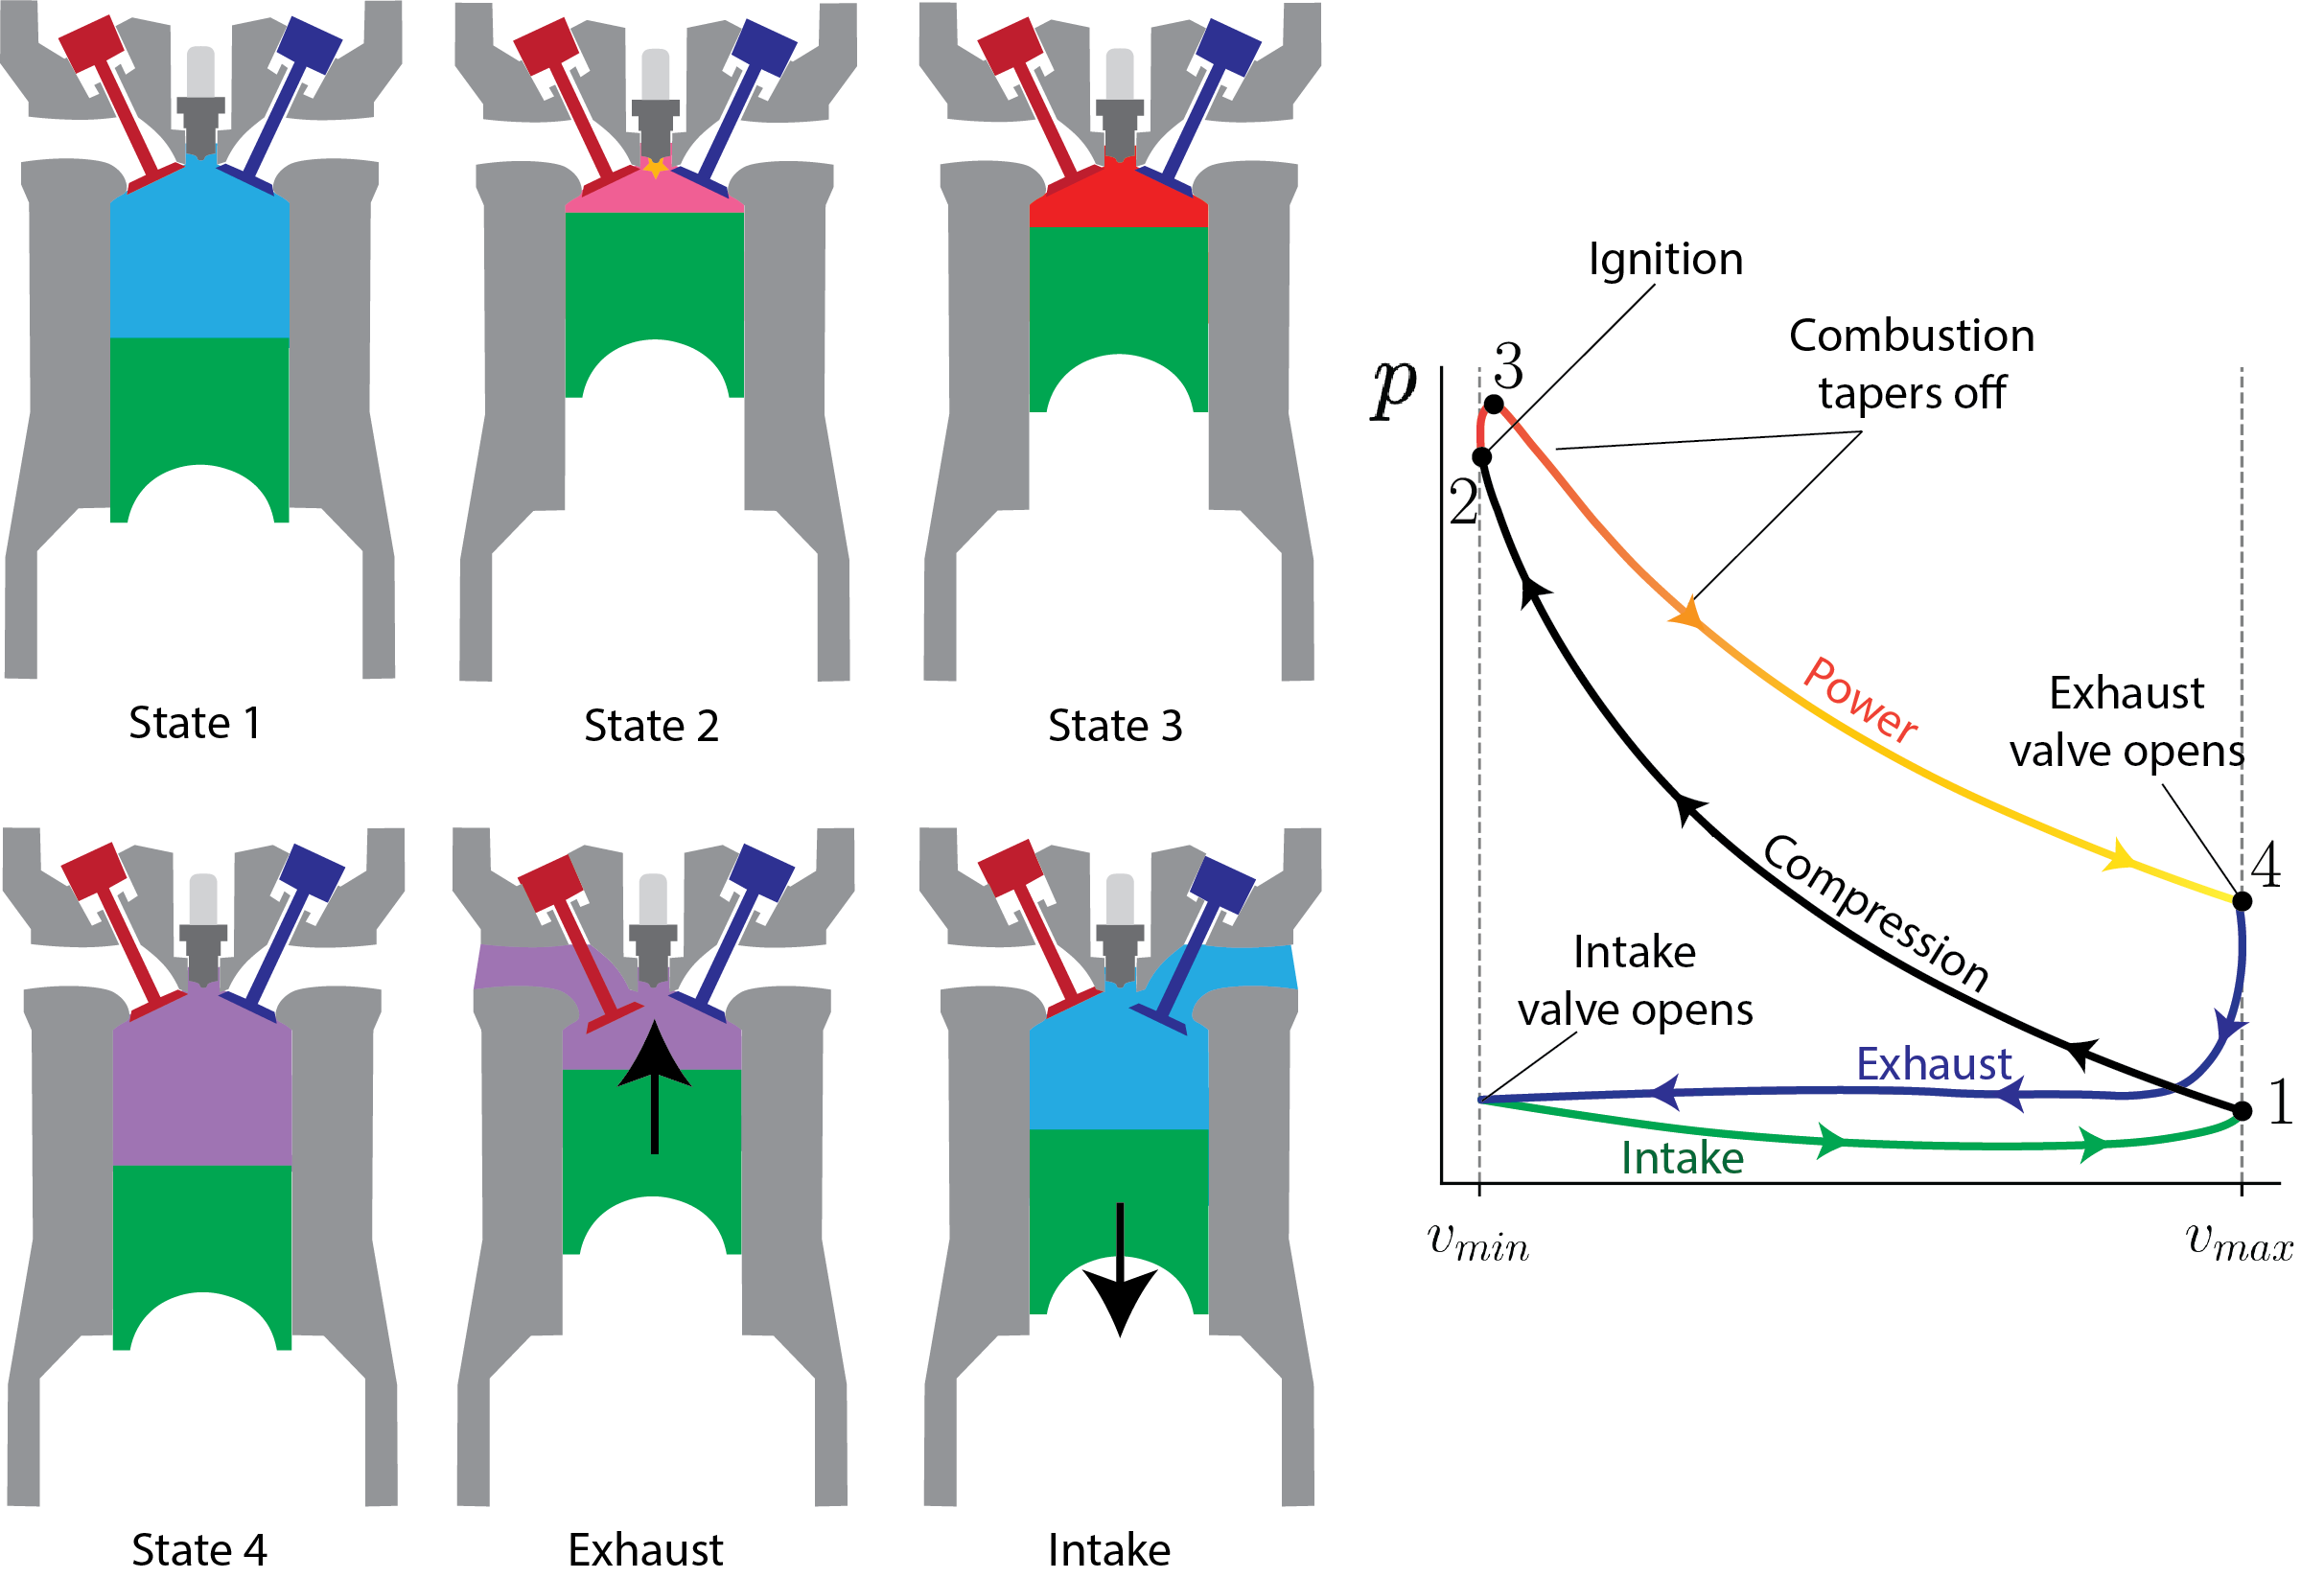
\includegraphics[width=0.9\textwidth]{FourStrokeCycle}
\caption{States of the four-stroke Otto Cycle with $p$-$v$ diagram.}
\label{fig:ch3_fourStroke}
\end{figure}

Figure \ref{fig:ch3_fourStroke} gives an approximate picture of an actual four-stroke spark-ignition cycle. It is extremely complex, both due to the gradual release of heat after ignition, as well as the mass transfer that occurs as the exhaust and intake valves open and close.  A perfect representation also needs to deal with the chemistry of combustion, the dynamics of fuel mixing, and the timing of various parts of the cycle.

Because the actual spark-ignition cycle is so complex, we make a number of simplifying assumptions.  First off, we use an ideal "air-standard" assumption, in which the working fluid is a fixed mass of air undergoing the complete cycle.  This simplification removes both the need for the exhaust/intake strokes and the need to consider the chemistry of combustion.  Instead of ignition, we use instantaneous heat addition between states 2 and 3.  Finally, the exhaust and intake strokes are replace by heat rejection between states 4 and 1.

\begin{figure}[H]
\centering
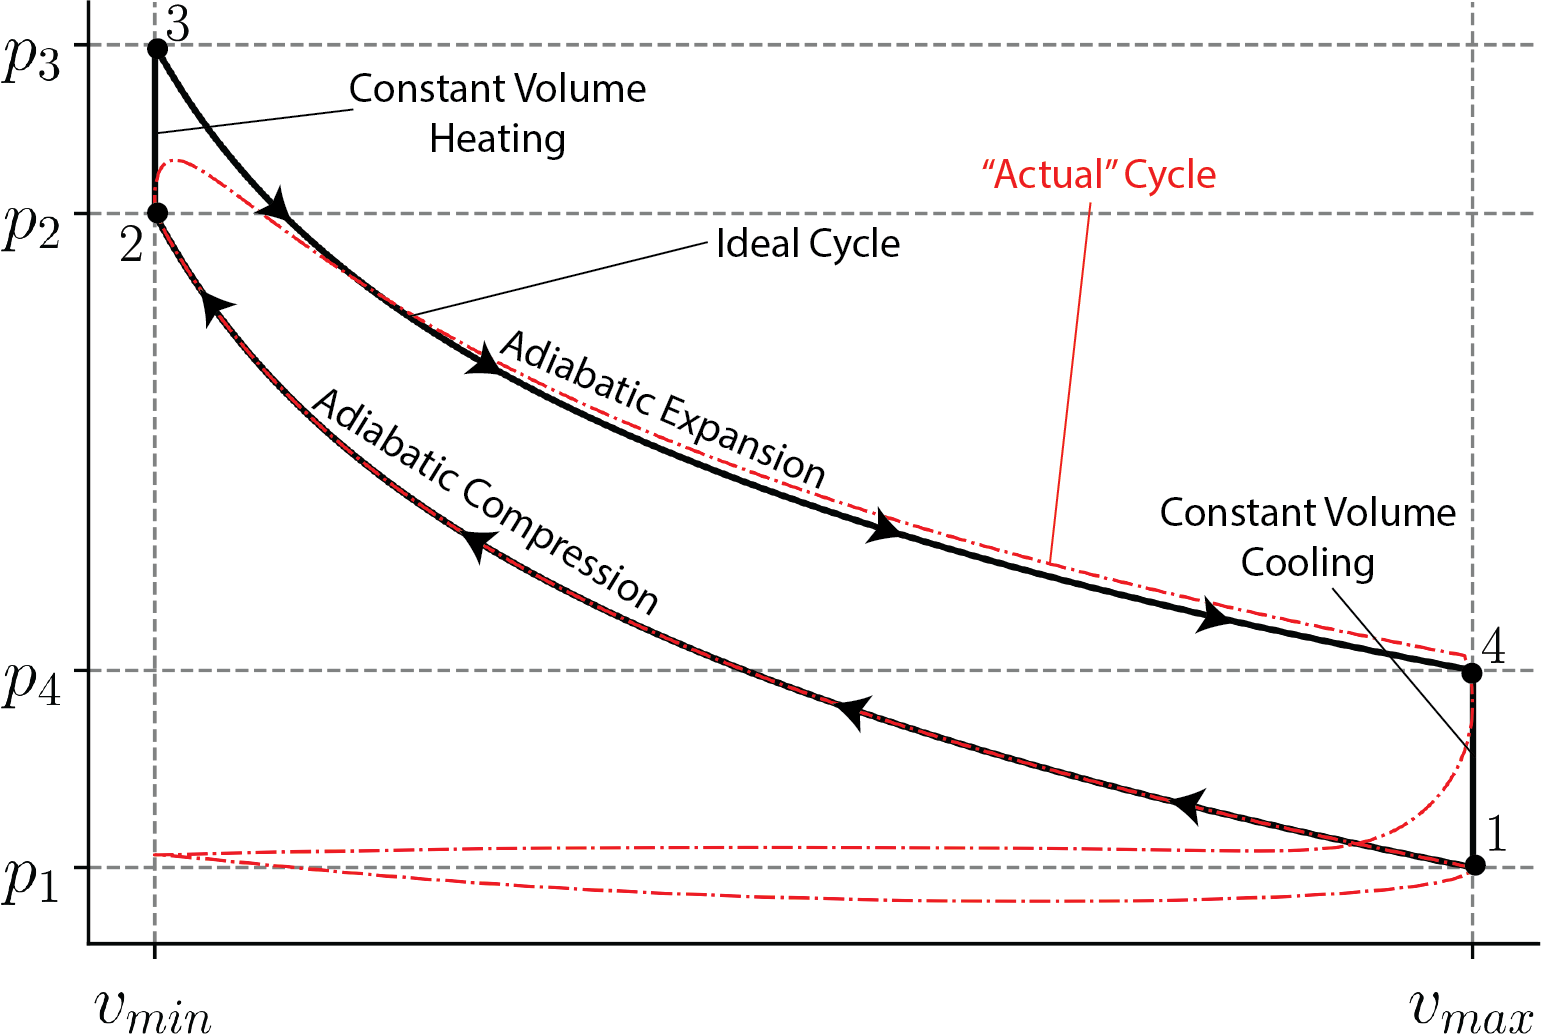
\includegraphics[width=0.75\textwidth]{OttoIdealCycle}
\caption{Ideal Otto cycle $p$-$v$ diagram compared to a simulated Otto cycle.}
\label{fig:ch3_ottoCycle}
\end{figure}

The end result is the cycle shown in Figure \ref{fig:ch3_ottoCycle}.  This looks very similar to the Stirling Cycle discussed in Section \ref{sec:ch3_stirling}.  The major difference between the two is that the compression between states 1 and 2 and the expansion between states 3 and 4 are both {\bf adiabatic}, rather than isothermal.  Analysis of these processes depends on the analysis done in Section \label{sec:ch3_idealGasAdiabatic}.

Note that the ideal cycle in Figure \ref{fig:ch3_ottoCycle} reaches significantly higher pressures than the actual cycle.  Additionally, the pressure at state 4 is slightly lower in the ideal cycle.  Both of these occur because of the assumption of instantaneous heat addition in the ideal cycle.  The actual cycle never reaches the high temperatures because expansion happens at the same time as heating, and the temperature is higher at state 4 because heat is added at a lower temperature, which means the air has a lower $c_v$ value.

The omission of the exhaust and intake strokes results in better efficiency for the ideal cycle, as work is required to both push out extra combustion products and to suck in fresh air. 
% --------------------------------------------------------------------
\subsection{Otto Cycle Analysis}

The Otto Cycle looks very similar to the Stirling Cycle discussed in Section \ref{sec:ch3_stirling}, with the key difference that the expansion and compression are adiabatic (no heat transfer) instead of isothermal.

The results of this can be seen in Table \ref{tab:ch3_otto}.  $\Delta u$ is always $c_v \Delta T$, though the definition of $\Delta T$ changes for each process.  For processes 1-2 and 3-4, $q=0$ because the processes are adiabatic.  For processes 2-3 and 4-1, $w=0$ because no work can be developed in a constant volume process.  The First Law ($\Delta u = q - w$) is used to fill in the remaining blanks.

\begin{table}[H]
  \centering
\def\arraystretch{1.5}
\caption{Tabular Representation of Energy Equation for the Otto Cycle}
\label{tab:ch3_otto}
\begin{tabular}{r|ccc}
            & $\Delta u$        & $q$             & $w$           \\ \hline
Process 1-2 & $ c_v (T_2-T_1)$ & 0                 &  $ -c_v (T_2-T_1)$ \\
Process 2-3 & $ c_v (T_3-T_2)$ & $ c_v (T_3-T_2)$   & 0       \\
Process 3-4 & $ c_v (T_4-T_3)$ & 0                 &  $ -c_v (T_4-T_3)$ \\ 
Process 4-1 & $ c_v (T_1-T_4)$ & $ c_v (T_1-T_4)$  &  0          \\ \hhline{=|===}
Total (net) & 0                 & $c_v (T_1-T_2+T_3-T_4)$ & $c_v (T_1-T_2+T_3-T_4)$
\end{tabular}
\def\arraystretch{1.0}
\end{table}

We are often interested in the {\bf thermal efficiency} of an engine, which is defined as $\eta_{th} = q_{in}/w_{net}$ in Equation \ref{eq:ch3_StirlingEfficiency}.  For the Otto engine, this becomes:
\begin{equation*}
  \eta_{th} = \frac{\cancel{c_v} \left(T_1-T_2+T_3-T_4\right)}{ \cancel{c_v} \left(T_3-T_2\right)} = 1 + \frac{T_1 - T_4}{T_3 - T_2}
\end{equation*}

Now we define the {\bf compression ratio}, $r$:
\begin{equation} \label{eq:ch3_comprat}
  r = \frac{v_{max}}{v_{min}}
\end{equation}
We can recognize that $v_{max}=v_1=v_4$ and $v_{min}=v_2=v_3$ to say that $r=v_1/v_2=v_4/v_3$.

We can then use the adiabatic relation for $T$ and $v$ from Equation \ref{eq:ch3_adiabaticTv} to make the following definitions:
\begin{align*}
  T_2 &= T_1 (v_2/v_1)^{-(\gamma-1)} = T_1 r^{\gamma-1}\\
  T_3 &= T_4 (v_3/v_4)^{-(\gamma-1)} = T_4 r^{\gamma-1}
\end{align*}

Using this, we can simplify the efficiency as follows:
\begin{align}
  \nonumber \eta_{th} &= 1 + \frac{ T_1-T_4}{ T_4 r^{\gamma-1} -T_1 r^{\gamma-1}} \\
  \nonumber \eta_{th} &= 1-\cancel{\frac{\left(T_4 - T_1\right)}{\left(T_4 - T_1\right)}} \frac{1}{r^{\gamma-1}} \\
  \label{eq:ch3_ottoeff} \eta_{th} &= 1 - \frac{1}{r^{\gamma-1}}
\end{align}

Equation \ref{eq:ch3_ottoeff} shows that the thermal efficiency is a function only of the compression ratio, $r$, and the ratio of specific heats, $\gamma$.  This simplified analysis requires the assumption that $\gamma$ is a constant over the entire cycle.  As long as $\gamma$ is chosen at or near $T_{avg}=\frac{1}{2}\left(T_{max}+T_{min}\right)$, this is a very reasonable assumption.

Example \ref{ex:ch3_otto} provides a closer look at an ideal Otto cycle.
\newpage
\begin{example}[label=ex:ch3_otto]{Otto Cycle}
  An ideal air-standard Otto cycle engine has a compression ratio of 8. At the beginning of the compression process, the working fluid is at 100 kPa, 27°C (300 K), and 800 kJ/kg heat is supplied during the constant volume heat addition process. Neatly sketch the pressure-volume [$p$-$v$] diagram for this cycle, and using the specific heat values for air at a typical average cycle temperature of 900 K determine:
\begin{enumerate}[a)]
\item the temperature and pressure of the air at the end of each process
\item the net work output/cycle [kJ/kg], and
\item the thermal efficiency [$\eta_{th}$] of this engine cycle.
\end{enumerate}

The first step is to draw the $p$-$v$ diagram of the complete cycle, including all the relevant information. We notice that neither volume nor mass have been provided, hence the diagram and solution will be in terms of specific quantities.

\begin{center}
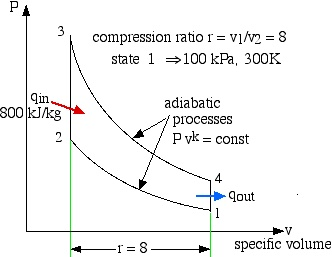
\includegraphics[width=0.65\textwidth]{OttoPV}
%\captionof{figure}{}
%\label{fig:ch2_example1}
\end{center}

We assume that the fuel-air mixture is represented by pure air. The relevant equations of state, internal energy and adiabatic process for air follow:
\begin{align*}
  pv&=RT & R &= 0.287 \frac{\rm kJ}{\rm kg\ K}\\
  \Delta u &= c_v \Delta T \\
  \frac{p_2}{p_1} &= \left(\frac{v_1}{v_2}\right)^{\gamma} & \frac{T_2}{T_1} &= \left(\frac{v_1}{v_2}\right)^{\gamma -1}
\end{align*}

Note that values for $c_v$ and $\gamma$ should come from the average value of temperature.  We won't know what the actual average temperature is until we solve the problem, but we are asked to use the ``typical average cycle temperature'' of 900 K.  We get this from the table of Specific Heat Capacities of Air.

\begin{equation*}
  c_{v,900\rm\ K} = 0.834 \frac{\rm kJ}{\rm kg\ K} \quad\quad\quad \gamma_{900\rm\ K} = 1.344
\end{equation*}

Compare these values to the nominal specific heat capacity values used for air at 300K: $C_v$ = 0.717 kJ/kg K and $\gamma$ = 1.4, and you will see the importance of using the Ideal Gas Tables.

We now go through all four processes in order to determine the temperature and pressure at the end of each process, as well as the work done and heat transferred during each process.

{\bf Process 1-2 - Adiabatic Compression:}
\begin{equation*}
  p_1 = 100\ {\rm kPa}, \quad \quad T_1 = 300\ {\rm K}
\end{equation*}
Starting at state 1, we compress the fluid adiabatically with a compression ratio of 8.  Keep in mind that the specific volume of state 1 will be {\bf larger} than that of state 2.
\begin{align*}
  &{\rm \bf Adiabatic} &\rightarrow& \redbox{q_{12} = 0\ \frac{\rm kJ}{\rm kg}} \\
  r &= \frac{v_1}{v_2} = 8 \\
  \frac{T_2}{T_1} &= \left(\frac{v_1}{v_2}\right)^{\gamma -1} = 8^{0.344} = 2.045 &\rightarrow & \redbox{T_2 = 613\ {\rm K}} \\
  \frac{p_2}{p_1} &= \left(\frac{v_1}{v_2}\right)^{\gamma} = 8^{1.344} = 16.359 &\rightarrow& \redbox{ p_2 = 1635\ {\rm kPa}}\\
\Delta u_{12} &= c_v \Delta T_{12} = \cancelto{0}{q_{12}} - w_{12} &\rightarrow& \redbox{w_{12} = -261\ \frac{\rm kJ}{\rm kg}}
\end{align*}

Note that we could also find the work through $\int p\: dv$.  The above approach is much simpler.

{\bf Process 2-3 - Constant Volume Combustion:}
From state 2, we add heat at constant volume ($v_3 = v_2$).
\begin{align*}
  &{\rm \bf Constant\ Volume} &\rightarrow& \redbox{w_{23} = 0\ \frac{\rm kJ}{\rm kg}} \\
   &{\rm \bf Given} &\rightarrow& \redbox{q_{23} = 800\ \frac{\rm kJ}{\rm kg}} \\
  q = c_v \Delta T \quad&\rightarrow\quad T_3 - T_2 = \frac{q}{c_v} \\
  T_3 - T_2 &= \frac{800\ \rm kJ/kg}{0.834\ \rm kJ/kgK} &\rightarrow &\redbox{T_3 = 1572 \ {\rm K}}\\
  \frac{p_3 }{p_2 } \frac{\cancel{v_3}}{\cancel{v_2}}&= \frac{\cancel{R}}{\cancel{R}}\frac{T_3}{T_2} &\rightarrow &\redbox{p_3 = 4193\ {\rm kPa}}
\end{align*}
\newpage
{\bf Process 3-4 - Adiabatic Expansion:}
From state 3 to 4, we again use the compression ratio, but recognize that $v_4 > v_3$.
\begin{align*}
  &{\rm \bf Adiabatic} &\rightarrow& \redbox{q_{34} = 0\ \frac{\rm kJ}{\rm kg}} \\
  r &= \frac{v_3}{v_4} = \frac{1}{8} \\
  \frac{T_4}{T_3} &= \left(\frac{v_3}{v_4}\right)^{\gamma -1} = \frac{1}{8}^{0.344} = 0.489 &\rightarrow &\redbox{T_3 = 769\ {\rm K}} \\
  \frac{p_4}{p_3} &= \left(\frac{v_3}{v_4}\right)^{\gamma} = \frac{1}{8}^{1.344} = 0.0611 &\rightarrow &\redbox{p_4 = 256\ {\rm kPa}} \\
  \Delta u_{12} &= c_v \Delta T_{12} = \cancelto{0}{q_{12}} - w_{12} &\rightarrow& \redbox{w_{34} = 670\ \frac{\rm kJ}{\rm kg}}
\end{align*}

{\bf Process 4-1 - Constant Volume Heat Rejection:}
From state 4, we reject heat at constant volume ($v_1 = v_4$).
\begin{align*}
  &{\rm \bf Constant\ Volume} &\rightarrow& \redbox{w_{23} = 0\ \frac{\rm kJ}{\rm kg}} \\
  \Delta u_{41} &= c_v \Delta T_{41} = q_{41} - \cancelto{0}{w_{12}} &\rightarrow& \redbox{q_{41} = -391\ \frac{\rm kJ}{\rm kg}}
\end{align*}

{\bf Cycle Summary:} Now we can build a summary of the processes using Table \ref{tab:ch3_otto}.
\begin{table}[H]
  \centering
\def\arraystretch{1.5}
%\caption{Tabular Representation of Energy Equation for Otto Cycle}
%\label{tab:ch3_stirling}
\begin{tabular}{r|ccc}
            & $\Delta U$        & $Q$      &$W$     \\ \hline
Process 1-2 & -261 kJ/kg        & 0 &  -261 kJ/kg  \\
Process 2-3 & 800 kJ/kg   & 800 kJ/kg & 0               \\
Process 3-4 & 670 kJ/kg   & 0              &  670 kJ/kg \\ 
Process 4-1 & -391 kJ/kg   &  -391 kJ/kg &  0  \\ \hhline{=|===}
Total (net) & 0                 &  409 kJ/kg & 409 kJ/kg
\end{tabular}
\def\arraystretch{1.0}
\end{table}

The net work created by a single cycle was 409 kJ/kg, and the heat added per cycle was 800 kJ/kg.  We can find the thermal efficiency as follows:
\begin{align*}
  \eta_{th} &= \frac{w_{net}}{q_{in}} = \frac{409\ {\rm kJ/kg}}{800\ {\rm kJ/kg}} &\rightarrow& \redbox{\eta_{th} = 51\%}
\end{align*}

Note that using constant specific heat values over the cycle we can determine the thermal efficiency directly from the ratio of specific heat capacities $\gamma$ and the compression ratio $r$ using Equation \ref{eq:ch3_ottoeff}:
\begin{equation*} 
  \eta_{th} = 1 - \frac{1}{r^{\gamma-1}} = 1 - \frac{1}{8^{0.344}}= 0.511
\end{equation*}
This matches closely with the analysis above.

\end{example}



% --------------------------------------------------------------------
\section{Air-Standard Diesel Cycle}
% --------------------------------------------------------------------

The Air Standard Diesel cycle is the ideal cycle for Spark-Ignition (CI) reciprocating engines, first proposed by Rudolph Diesel over 100 years ago. The following link by the Kruse Technology Partnership describes the \href{http://www.kruse-ltc.com/diesel.php}{four-stroke diesel cycle} operation including a short history of Rudolf Diesel. The four-stroke diesel engine is usually used in motor vehicle systems, whereas larger marine systems usually use the \href{https://auto.howstuffworks.com/diesel-two-stroke1.htm}{two-stroke diesel cycle}. Once again we have an excellent animation produced by Matt Keveney presenting the operation of the \href{http://animatedengines.com/diesel.html}{four-stroke diesel cycle}.

The analysis of the Diesel cycle is very similar to that of the Otto cycle which we analyzed in the previous section. We will use the ideal "air-standard" assumption in our analysis. Thus the working fluid is a fixed mass of air undergoing the complete cycle which is treated throughout as an ideal gas. All processes are ideal, combustion is replaced by heat addition to the air, and exhaust is replaced by a heat rejection process which restores the air to the initial state.

\begin{figure}[H]
\centering
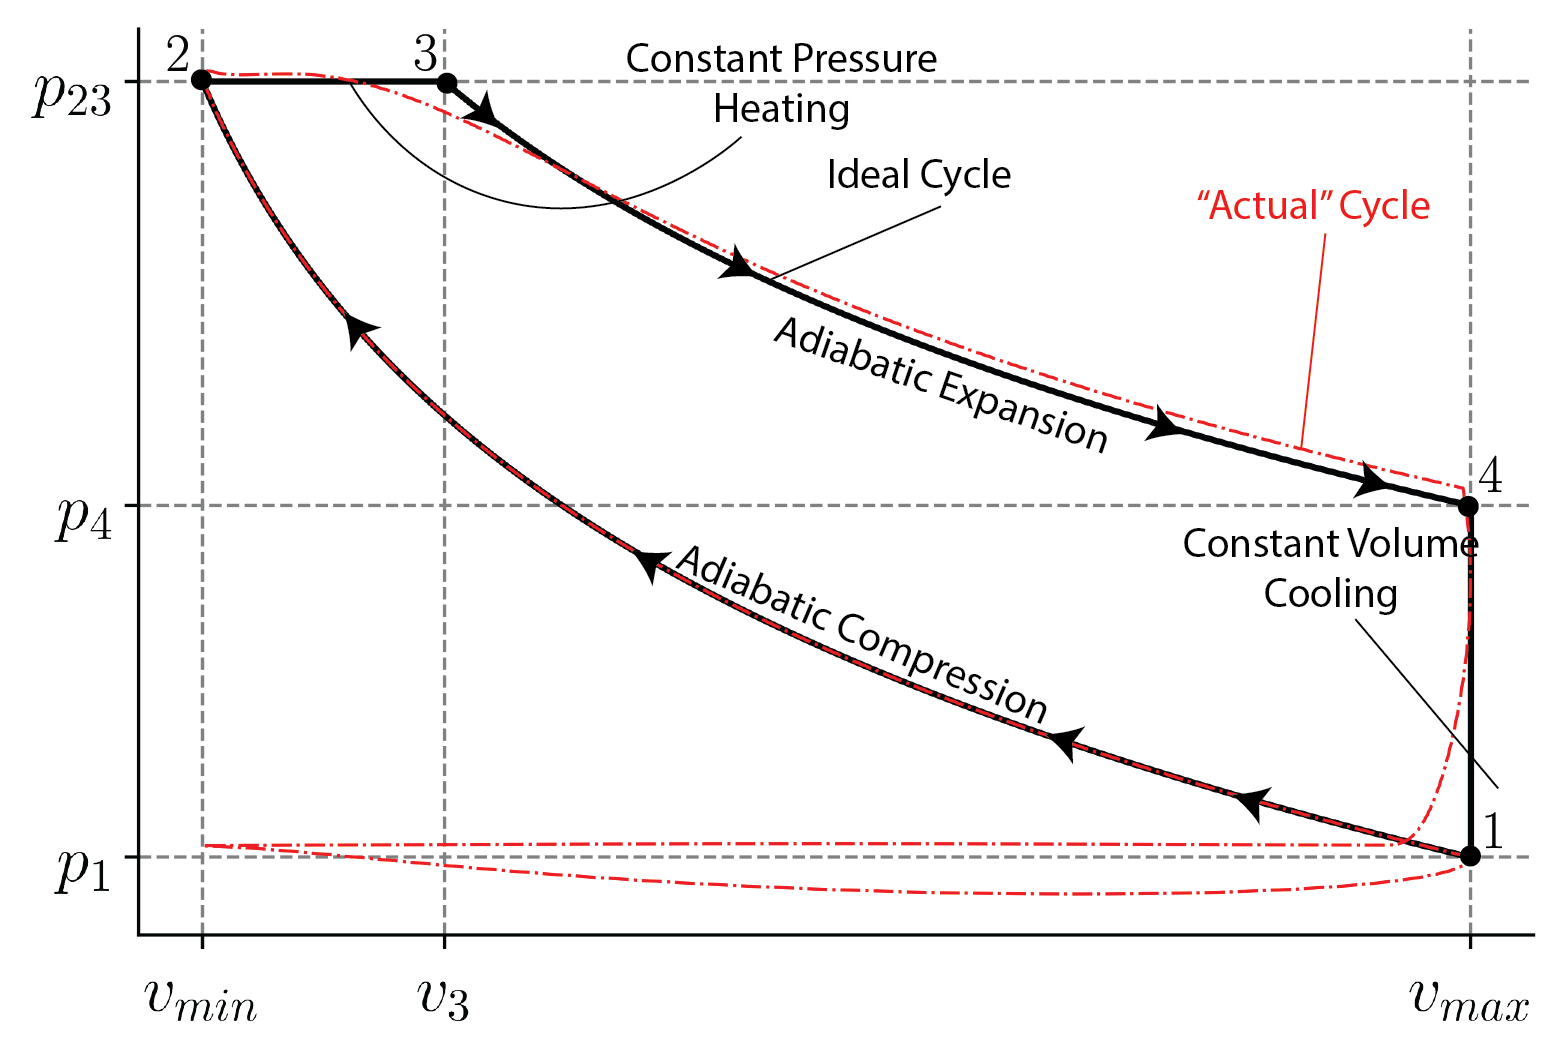
\includegraphics[width=0.75\textwidth]{DieselIdealCycle}
\caption{Ideal Diesel Cycle $p$-$v$ diagram compared to a simulated Diesel Cycle.}
\label{fig:ch3_dieselCycle}
\end{figure}

The most significant difference between the ideal Otto cycle and the ideal Diesel cycle is the method of igniting the fuel-air mixture.  For the Otto cycle, spark-ignition allows us to maintain a relatively low compression ratio (around 8:1), and time the combustion such that it results in a sudden jump in pressure while the volume remains essentially constant.

In contrast, in order to self-ignite, the ideal Diesel cycle needs an extremely high compression ratio (around 18:1) to allow the air to reach the ignition temperature of the fuel. Only then is the fuel injected.  The timing of ignition is such that combustion adds heat as the piston is in the process of expanding, which leads to combustion at nearly a constant pressure, as seen in Figure \ref{fig:ch3_dieselCycle}.

After combustion, the rest of the cycle (expansion and exhaust) is essentially identical to that of the ideal Otto cycle.

\subsection{Diesel Cycle Analysis}

The Diesel cycle is very similar to the Otto cycle, with the major change that heating occurs at constant pressure, rather than constant volume.  The major complication is that work occurs at the same time as heat transfer, unlike in the Otto cycle, where work and heat transfer are perfectly decoupled.

\begin{table}[H]
  \centering
\def\arraystretch{1.5}
\caption{Tabular Representation of Energy Equation for the Diesel Cycle}
\label{tab:ch3_diesel}
\begin{tabular}{r|ccc}
            & $\Delta u$        & $q$             & $w$           \\ \hline
Process 1-2 & $ c_v (T_2-T_1)$ & 0                 &  $ -c_v (T_2-T_1)$ \\
Process 2-3 & $ c_v (T_3-T_2)$ & $ c_p (T_3-T_2)$   & $p_{23} (v_3 - v_2) = R(T_3-T_2)$ \\
Process 3-4 & $ c_v (T_4-T_3)$ & 0                 &  $ -c_v (T_4-T_3)$ \\ 
Process 4-1 & $ c_v (T_1-T_4)$ & $ c_v (T_1-T_4)$  &  0          \\ \hhline{=|===}
Total (net) & 0                 & $c_v (T_1-T_4)+c_p(T_3-T_2)$ & $c_v (T_1-T_4) + c_p(T_3-T_2)$
\end{tabular}
\def\arraystretch{1.0}
\end{table}

Let's again find the thermal efficiency:
\begin{equation*}
  \eta_{th} = \frac{c_v \left(T_1-T_4\right)+c_p\left(T_3-T_2\right)}{ c_p \left(T_3-T_2\right)} = 1-\frac{\left(T_4-T_1\right)}{\gamma \left(T_3-T_2\right)}
\end{equation*}

Often, rather than indicating the amount of heat from combustion, the heat addition process is defined by a {\bf cutoff ratio}.  This is another volume ratio, defined as:
\begin{equation} \label{eq:ch3_cutoffRatio}
  r_c = \frac{v_3}{v_2}
\end{equation}

The cutoff ratio will always be less than the compression ratio (Equation \ref{eq:ch3_compressionRatio}).  Additionally, this ratio allows us to link each of our temperatures using $r$, $r_c$, and $\gamma$:
\begin{align*}
  T_2 &= T_1\: r^{\gamma-1}  &\quad& \text{from adiabatic relations}\\
  T_3 &= T_2\: r_c &\quad& \text{from the ideal gas law}\\
  T_4 &= T_3 \left(\frac{r_c}{r}\right)^{\gamma-1} &\quad& \text{from adiabatic relations}
\end{align*}

We can simplify $T_3$ and $T_4$ as follows:
\begin{align*}
  T_3 &= T_1\: r^{\gamma-1}\: r_c \\
  T_4 &= T_1\: \cancel{r^{\gamma-1}}\: r_c \left(\frac{r_c}{\cancel{r}}\right)^{\gamma-1} = T_1 r_c r_c^{\gamma-1} = T_1 r_c^{\gamma}
\end{align*}

Substituting the above relationships into the thermal efficiency gives us the following:
\begin{align}
  \nonumber \eta_{th} &= 1 - \frac{T_1 r_c^{\gamma} - T_1}{\gamma \left(T_1 \: r^{\gamma-1}\: r_c -  T_1\: r^{\gamma-1}\right)} \\
  \label{eq:ch3_dieseleff} \eta_{th} &= 1 - \frac{1}{\gamma\:r^{\gamma-1}}\frac{r_c^{\gamma} - 1}{r_c -  1}
\end{align}

As $r_c\rightarrow 1$, Equation \ref{eq:ch3_dieseleff} approaches Equation \ref{eq:ch3_ottoeff}, the Otto efficiency.

Example \ref{ex:ch3_diesel} provides a closer look at an ideal Diesel cycle.

\begin{example}[label=ex:ch3_diesel]{Diesel Cycle}
  An ideal air-standard Diesel cycle engine has a compression ratio of 18 and a cutoff ratio of 2. At the beginning of the compression process, the working fluid is at \mbox{100 kPa}, 27°C (300 K).
\begin{enumerate}[a)]
\item Determine the temperature and pressure of the air at the end of each process.
\item Determine the net work output per cycle [kJ/kg].
\item Determine the thermal efficiency.
\end{enumerate}

The first step is to draw a diagram representing the problem, including all the relevant information. We notice that neither volume nor mass is given, hence the diagram and solution will be in terms of specific quantities. The most useful diagram for a heat engine is the $p$-$v$ diagram of the complete cycle:

\begin{center}
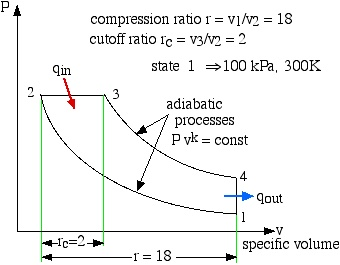
\includegraphics[width=0.75\textwidth]{DieselPv}
%\captionof{figure}{}
%\label{fig:ch2_example1}
\end{center}

In order to use constant specific heats, we must guess the average temperature of the cycle.  For this analysis, we will use 900 K to calculate the specific heats.  We will then check that value at the end of the analysis.

\begin{equation*}
  c_{p,900\rm\ K} = 1.121\ \frac{\rm kJ}{\rm kg\ K} \quad\quad\quad \gamma_{900\rm\ K} = 1.344
\end{equation*}

We now go through all four processes in order to determine the temperature and pressure at the end of each process, as well as the work done and heat transferred during each process.

{\bf Process 1-2 - Adiabatic Compression:}
\begin{equation*}
  p_1 = 100\ {\rm kPa}, \quad \quad T_1 = 300\ {\rm K}
\end{equation*}
Starting at state 1, we compress the fluid adiabatically with a compression ratio of 18.  Keep in mind that the specific volume of state 1 will be {\bf larger} than that of state 2.
\begin{align*}
  &{\rm \bf Adiabatic} &\rightarrow& \redbox{q_{12} = 0\ \frac{\rm kJ}{\rm kg}} \\
  r &= \frac{v_1}{v_2} = 18 \\
  \frac{T_2}{T_1} &= \left(\frac{v_1}{v_2}\right)^{\gamma -1} = 18^{0.344} = 2.703 &\rightarrow & \redbox{T_2 = 811\ {\rm K}} \\
  \frac{p_2}{p_1} &= \left(\frac{v_1}{v_2}\right)^{\gamma} = 18^{1.344} = 48.650 &\rightarrow& \redbox{ p_2 = 4865\ {\rm kPa}}%\\
%\Delta u_{12} &= c_v \Delta T_{12} = \cancelto{0}{q_{12}} - w_{12} &\rightarrow& \redbox{w_{12} = -261 \frac{\rm kJ}{\rm kg}}
\end{align*}

{\bf Process 2-3 - Constant Pressure Combustion:}
From state 2, we add heat at constant pressure ($p_3 = p_2$), with a cutoff ratio of 2.
\begin{align*}
  &{\rm \bf Constant\ Pressure}  &\rightarrow& \redbox{p_3 = 4865\ {\rm kPa}} \\
  \frac{\cancel{p_3}}{\cancel{p_2} } \cancelto{2}{\frac{v_3}{v_2}}&= \frac{\cancel{R}}{\cancel{R}}\frac{T_3}{T_2} &\rightarrow &\redbox{T_3 = 1622\ {\rm K}}
\end{align*}
For this process, both work and heat transfer are present.  However, we can find the heat transfer by using the constant pressure specific heat, $c_p$:
\begin{align*}
    q_{23} = c_p (T_3 - T_2) =1.121\ \frac{\rm kJ}{\rm kg\ K} \cdot \left(1622\ {\rm K} - 811\ {\rm K}\right)\quad&\rightarrow& \redbox{q_{23} = 909\ \frac{\rm kJ}{\rm kg}}
\end{align*}

{\bf Process 3-4 - Adiabatic Expansion:}
To calculate the volume ratio between states 3 and 4, we simply divide the compression ratio by the cutoff ratio:
\begin{equation*}
  \frac{v_4}{v_3} = \frac{v_1}{v_3} = \frac{v_2}{v_3}\frac{v_1}{v_2} = \frac{r}{r_c}
\end{equation*}
This allows us to follow a similar pattern to Process 1-2.
\begin{align*}
  &{\rm \bf Adiabatic} &\rightarrow& \redbox{q_{34} = 0\ \frac{\rm kJ}{\rm kg}} \\
  \frac{v_3}{v_4} = \frac{r_c}{r}=\frac{1}{9} \\
  \frac{T_4}{T_3} &= \left(\frac{v_3}{v_4}\right)^{\gamma -1} = \frac{1}{9}^{0.344} = 0.470 &\rightarrow &\redbox{T_3 = 762\ {\rm K}} \\
  \frac{p_4}{p_3} &= \left(\frac{v_3}{v_4}\right)^{\gamma} = \frac{1}{8}^{1.344} = 0.0522 &\rightarrow &\redbox{p_4 = 254\ {\rm kPa}}
\end{align*}

{\bf Process 4-1 - Constant Volume Heat Rejection:}
From state 4, we reject heat at constant volume ($v_1 = v_4$).
\begin{align*}
  \Delta u_{41} &= c_v \Delta T_{41} = q_{41} - \cancelto{0}{w_{12}} &\rightarrow& \redbox{q_{41} = -385\ \frac{\rm kJ}{\rm kg}}
\end{align*}

{\bf Cycle Summary:} Notice that we didn't calculate the work for any of the processes.  The reason for this is we can more easily obtain the net work, $w_{net}$, by finding the net heat transfer, $q_{net}$.  For a cycle, the net work and the net heat transfer will be equal.
\begin{equation*}
  w_{net} = q_{net} = 909\ \frac{\rm kJ}{\rm kg} - 385\ \frac{\rm kJ}{\rm kg} \quad \rightarrow \quad \redbox{w_{net} = 524\ \frac{\rm kJ}{\rm kg}}
\end{equation*}

We can find the thermal efficiency as follows:
\begin{align*}
  \eta_{th} &= \frac{w_{net}}{q_{in}} = \frac{524\ {\rm kJ/kg}}{909\ {\rm kJ/kg}} &\rightarrow& \redbox{\eta_{th} = 58\%}
\end{align*}

As a side note, our maximum temperature was about 1600 K, so an average temperature of 900 K for finding $c_p$ and $\gamma$ is reasonable.

You may wonder at the unrealistically high thermal efficiency obtained in this example. In this idealized analysis we have ignored many loss effects that exist in practical heat engines. We will begin to understand some of these loss mechanisms when we study the Second Law in Chapter 5.
\end{example}

\section{Using Software: Plotting a Cycle in Python}
In Section \ref{sec:ch1_colab}, we introduced the various plotting options available in Python through \href{https://colab.research.google.com}{Google Colab}.  In Section \ref{sec:ch2_colab}, we used Colab in order to implement the ideal gas law.

In this section, we will combine the two in order to plot the Otto cycle in Python.

\subsection{Solving the Otto Cycle in Colab}
To start off, let's solve Example 3.5 in Colab.  We still need to start off by including our library imports:

\begin{Verbatim}[commandchars=\\\{\}]
\textcolor{OliveGreen}{# Clear all variable definitions}
\textcolor{blue}{\%reset} -f                         
\textcolor{violet}{from} numpy \textcolor{violet}{import} *               \textcolor{OliveGreen}{# Import common numerical functions (like sqrt)}
\textcolor{violet}{from} matplotlib.pyplot \textcolor{violet}{import} *   \textcolor{OliveGreen}{# Import plotting functions (like plot)}
\textcolor{violet}{import} CoolProp.CoolProp \textcolor{violet}{as} CP    \textcolor{OliveGreen}{# Import CoolProp library}
\end{Verbatim}

With those in place, we define the known values for this Otto cycle:
\begin{Verbatim}[commandchars=\\\{\}]
\textcolor{OliveGreen}{# Given Values}                
cv    = \textcolor{JungleGreen}{0.834}      \textcolor{OliveGreen}{# Constant volume specific heat for air at 900 K (kJ/kgK)}
gamma = \textcolor{JungleGreen}{1.344}      \textcolor{OliveGreen}{# Ratio of specific heats for air at 900 K (-)}
Rgas = \textcolor{JungleGreen}{8.314}/\textcolor{JungleGreen}{28.97} \textcolor{OliveGreen}{# Gas constant for air (kJ/kgK)}
r = \textcolor{JungleGreen}{8}              \textcolor{OliveGreen}{# Compression ratio of cycle (-)}
qin = \textcolor{JungleGreen}{800}          \textcolor{OliveGreen}{# Combustion heat transfer (kJ/kg)}
T1 = \textcolor{JungleGreen}{300}           \textcolor{OliveGreen}{# Initial temperature (K)}
p1 = \textcolor{JungleGreen}{100}           \textcolor{OliveGreen}{# Initial pressure (kPa)}
\end{Verbatim}

The compression ratio is our path to state 2, so we need to start off by finding the specific volume of state 1:

\begin{Verbatim}[commandchars=\\\{\}]
\textcolor{OliveGreen}{# Find v2}                
v1 = Rgas * T1 / p1  \textcolor{OliveGreen}{# Ideal Gas Law}
v2 = v1 / r          \textcolor{OliveGreen}{# compression ratio r = v1/v2}
\end{Verbatim}

The pressure and temperature of state 2 can be found using the adiabatic ideal gas equations (Equations \ref{eq:ch3_adiabaticIdealGasTV} and \ref{eq:ch3_adiabaticIdealGaspV}):

\begin{Verbatim}[commandchars=\\\{\}]
\textcolor{OliveGreen}{# Find p2 and T2 with adiabatic ideal gas equations}                
T2 = T1 * (v1/v2)**(gamma-1)
p2 = p1 * (v1/v2)**gamma  
\end{Verbatim}

The volume at state 3 is the same as at state 2.  The temperature at state 3 is found using the equation for constant-volume heat addition.  The pressure can be found through the ideal gas law.
\begin{Verbatim}[commandchars=\\\{\}]
\textcolor{OliveGreen}{# Find values of state 3 (constant volume heat addition)}                
v3 = v2             \textcolor{OliveGreen}{# constant volume process}
T3 = T2 + qin/cv    \textcolor{OliveGreen}{# q = cv*deltaT}
p3 = T3*Rgas/v3     \textcolor{OliveGreen}{# Ideal gas law}
\end{Verbatim}

The volume at state 4 is the same as state 1.  The temperature and pressure can be found through the adiabatic ideal gas law equations.

\begin{Verbatim}[commandchars=\\\{\}]
\textcolor{OliveGreen}{# Find p4 and T4 with adiabatic ideal gas equations}                
v4 = v1
T4 = T3 * (v3/v4)**(gamma-1)
p4 = p3 * (v3/v4)**gamma  
\end{Verbatim}

At this point, we have each of our four states fully defined.  If we want to know the values, we can use the print command:

\begin{Verbatim}[commandchars=\\\{\}]
\textcolor{OliveGreen}{# Output state values}                
print(\textcolor{purple}{'State    Pressure    Temperature    Spec. Volume'})
print(\textcolor{purple}{'  1     %9.3f    %9.3f    %9.3f'}% (p1, T1, v1))
print(\textcolor{purple}{'  2     %9.3f    %9.3f    %9.3f'}% (p2, T2, v2))
print(\textcolor{purple}{'  3     %9.3f    %9.3f    %9.3f'}% (p3, T3, v3))
print(\textcolor{purple}{'  4     %9.3f    %9.3f    %9.3f'}% (p4, T4, v4))
\end{Verbatim}

This set of commands gives us the following table:
\begin{verbatim}
State    Pressure    Temperature    Spec. Volume
  1       100.000      300.000        0.861
  2      1635.886      613.457        0.108
  3      4193.839     1572.690        0.108
  4       256.365      769.095        0.861
\end{verbatim}

This print command looks a lot different than what we've used in the past.  Instead of manually putting in each of the values we wanted to print, we used {\bf placeholders}, which were then filled after we completed the format.  This allows us to create a small table without having to spend a ton of time fidgeting with spacing.

The placeholders have three components:
\begin{itemize}
\item The first value (9) indicates how much total space to give the number.  A smaller number will provide less white space.  If the number requires more space than given, Python will automatically give as much as needed (which would mess up our table).
\item The second piece (.3) indicates the precision, or how many numbers after the decimal point will be included.
\item The final piece (f) is an argument or conversion specifier.  You may want to use \verb~%9.3e~ instead for very large or small numbers to use an exponential format (e.g. \verb~4.194e+03~ instead of \verb~4193.839~).
\end{itemize}

\subsection{Plotting the States}
With our states fully known, let's plot the properties on a $p$-$v$ diagram.

We only have four values, so we can create our list manually:

\begin{verbatim}
plot([v1, v2, v3, v4], [p1, p2, p3, p4])
\end{verbatim}

This results in the following plot:
\begin{center}
\includegraphics[width=0.6\textwidth]{initialPVDiagram}
%\captionof{figure}{}
%\label{fig:ch2_example1}
\end{center}

This plot has a number of issues.  We need labels and better limits for the axes, the cycle doesn't make a full circuit, and the adiabatic compression and expansion are straight lines, rather than following the path they should.
Additionally, it would be nice to label each of the states with a number.  Let's tackle each of these.
\subsection{Revising the Plot}
\subsubsection{Axis Labels and Limits}
We've done this before in Section \ref{sec:ch1_colab}, but to re-cap, we'll use the \verb~xlabel~, \verb~ylabel~, and \verb~axis~ commands.
\begin{Verbatim}[commandchars=\\\{\}]
xlabel(\textcolor{purple}{'Spec. Volume [m^3/kg]'})
ylabel(\textcolor{purple}{'Pressure [kPa]'})
axis([\textcolor{ForestGreen}{0}, \textcolor{ForestGreen}{1}, \textcolor{ForestGreen}{0}, \textcolor{ForestGreen}{4500}])
\end{Verbatim}

\subsubsection{Adiabatic Compression/Expansion Lines} \label{sec:plottingCurvedLines}
This one is a bit more difficult.  In order to create curved lines, we need to create an array to work with.  We know the limits of specific volume, so we'll use that as our base.
\begin{Verbatim}[commandchars=\\\{\}]
vArray = linspace(v2, v1, \textcolor{ForestGreen}{100})
\end{Verbatim}

Once we have that in hand, we want define our pressure array by substituting the volume array for $v_2$ in Equation \ref{eq:ch3_adiabaticIdealGaspV}.

\begin{Verbatim}[commandchars=\\\{\}]
pArrayComp = p1*(vArray/v1)**-gamma
\end{Verbatim}

We can do the exact same thing for the expansion stroke by substituting $p_1$ for $p_3$ and $v_1$ for $v_3$:
\begin{Verbatim}[commandchars=\\\{\}]
pArrayExp = p3*(vArray/v3)**-gamma
\end{Verbatim}

Let's add two plot commands to plot these two lines, making them both blue.
\begin{Verbatim}[commandchars=\\\{\}]
plot(vArray, pArrayComp, \textcolor{purple}{'b'})
plot(vArray, pArrayExp, \textcolor{purple}{'b'})
\end{Verbatim}

\subsubsection{Adding State Labels}

To label the states, we use matplotlib's \verb~text~ command:

\begin{Verbatim}[commandchars=\\\{\}]
text(v1+.01, p1-50, \textcolor{purple}{'1'})  \textcolor{OliveGreen}{# Place the text '1' next to state 1}
text(v2-.03, p2-50, \textcolor{purple}{'2'})
text(v3-.03, p3+50, \textcolor{purple}{'3'})
text(v4+.01, p4+50, \textcolor{purple}{'4'})
\end{Verbatim}

The first two arguments tell Colab where to place the text, and the third argument is what text to type.  This can be finicky, and the easiest way to determine correct placement is just to alter the values added or subtracted from the specific volume and pressure.

After all of the changes above, we end up with the following:
\begin{center}
\includegraphics[width=0.6\textwidth]{secondPVDiagram}
%\captionof{figure}{}
%\label{fig:ch2_example1}
\end{center}

\subsubsection{Finishing Up}
To clean up the plot, we want to get rid of our original lines and manually put in the lines for constant volume heating and cooling.

For the first bit, we'll change our lines to simple circles by adding \verb~'ob'~ to the end of the plot command.  The \verb~o~ piece makes small circles instead of the lines, while \verb~b~ keeps the circles blue.

The command becomes:
\begin{Verbatim}[commandchars=\\\{\}]
plot([v1, v2, v3, v4], [p1, p2, p3, p4], \textcolor{purple}{'ob'})
\end{Verbatim}

In order to create the constant volume lines, we just connect the two points:
\begin{Verbatim}[commandchars=\\\{\}]
plot([v2, v3], [p2, p3], \textcolor{purple}{'b'})
plot([v4, v1], [p4, p1], \textcolor{purple}{'b'})
\end{Verbatim}

After all this, we end up with the final plot:
\begin{center}
\includegraphics[width=0.6\textwidth]{finalPVDiagram}
%\captionof{figure}{}
%\label{fig:ch2_example1}
\end{center}

\subsubsection{Semi-log Plots}
There's an argument for using semi-log or log-log plots, depending on differences in pressure.

Replacing all of the \verb~plot~ commands with \verb~semilogy~ and changing the y-axis from a $0<p<4500$ to $50<p<5000$ yields the following plot:

\begin{center}
\includegraphics[width=0.6\textwidth]{finalPVDiagramSemilog}
%\captionof{figure}{}
%\label{fig:ch2_example1}
\end{center}

In order for the plot to come out well, it is also necessary to fiddle with the \verb~text~ commands.  In addition, to fix the tick labels on the $y$ axis, it is also necessary to add a \verb~yticks~ command:
\begin{Verbatim}[commandchars=\\\{\}]
yticks(ticks=[\textcolor{ForestGreen}{50}, \textcolor{ForestGreen}{100}, \textcolor{ForestGreen}{200}, \textcolor{ForestGreen}{500}, \textcolor{ForestGreen}{1000}, \textcolor{ForestGreen}{2000}, \textcolor{ForestGreen}{5000}], 
       labels=[\textcolor{ForestGreen}{50}, \textcolor{ForestGreen}{100}, \textcolor{ForestGreen}{200}, \textcolor{ForestGreen}{500}, \textcolor{ForestGreen}{1000}, \textcolor{ForestGreen}{2000}, \textcolor{ForestGreen}{5000}])
\end{Verbatim}

\section{Summary}
The main result from this chapter was the explanation of three engine cycles: Stirling, Otto, and Diesel.  Each of these cycles can convert excess heat, typically from combustion, to work.  The Stirling cycle can also use work in order to transfer heat from a cold environment to a hot environment, thus acting as either a heater or a refrigerator.  All of these cycles typically use ideal gases as the working fluid, so the ideal gas law was used in abundance.

In order to analyze these cycles, we introduced the First Law of Thermodynamics:
\begin{equation*}
  \Delta U = Q - W,
\end{equation*}
which is a statement of the conservation of energy.  The change in internal energy can be determined from the temperature change between states:
\begin{align*}
  \Delta U = U_2 - U_1 &= m c_v (T_2 - T_1) & \Delta u = u_2 - u_1 &= c_v (T_2 - T_1)
\end{align*}
The work is typically found through integration, which results in the following for special cases:
\begin{align*}
  {\rm Isobaric} & &\rightarrow& & W &= mp (v_2 - v_1) = p(V_2 - V_1)\\
  {\rm Isothermal} & &\rightarrow& & W &= mRT \ln \left(\frac{v_2}{v_1}\right)  = mRT \ln \left(\frac{V_2}{V_1}\right)\\
  {\rm Adiabatic} & &\rightarrow& & W &= m\:\frac{p_1 v_1 - p_2 v_2}{\gamma - 1} = m c_v (T_2-T_1)\\
  {\rm Isometric} & &\rightarrow& & W &= 0
\end{align*}

For the special case of constant pressure, the heat transfer for a process can be found using the constant pressure specific heat, $c_p$:

\begin{equation*}
  Q = m c_p (T_2 - T_1)
\end{equation*}

In all other circumstances, the heat transfer can only be determined through the First Law.

Finally, because two of the cycles use adiabatic compression/expansion, it was necessary to develop equations for the properties.  These are summarized below:

\begin{align*}
  \frac{p_2}{p_1} &= \left(\frac{T_2}{T_1}\right)^{\frac{\gamma}{\gamma -1}} = \left(\frac{v_1}{v_2}\right)^{\gamma} \\
  \frac{T_2}{T_1} &= \left(\frac{p_2}{p_1}\right)^{\frac{\gamma-1}{\gamma}} = \left(\frac{v_1}{v_2}\right)^{(\gamma -1)} \\
  \frac{v_2}{v_1} &= \left(\frac{p_1}{p_2}\right)^{\frac{1}{\gamma}} = \left(\frac{T_1}{T_2}\right)^{\frac{1}{(\gamma -1)}}
\end{align*}

\begin{homework}
  %{\bf Conceptual Questions}
  % Section 3.1 - First Law
  \question Look at Figure \ref{fig:ch3_pV}.  Which process would require the most work to complete?  What does this say about the heat transfer during that process?
  
  \question Why is work negative in the First Law of Thermodynamics?

  % Section 3.2 - Enthalpy
  \question In what circumstances is enthalpy useful?  In other words, why would we use enthalpy instead of internal energy?
  
  \question Which is larger, internal energy or enthalpy?  Is this always true?  Why?

  % Section 3.3 - Specific Heats
  \question In what ways is specific heat different between gases and solids?
  
  \question In words, what is $c_p$?

  % Section 3.4 - Stirling Cycle Engine
  \question What is the function of the regenerator?  Without a regenerator, what would be the effect on the engine?
  
  \question Is there heating that occurs during constant temperature expansion/compression?  If so, how much?
  
  % Section 3.5 - Stirling Cycle Cooling
  \question Draw the cycles in a $p$-$v$ diagram for the Stirling Cycle Engine and Stirling Cycle Cooler.  What is different between the two? Label all heat flow and work in and out of the the system.  Use $Q_H$, $Q_C$, $Q_R$, $W_{in}$, and $W_{out}$ for your labels.

  % Section 3.6 - Ideal Gas Adiabatic Processes
  \question What is $\gamma$?  How does it change with temperature (see Table \ref{sec:idealGasAir})?
  
  \question What assumptions are necessary to use Equations \ref{eq:ch3_adiabaticIdealGasTV}, \ref {eq:ch3_adiabaticIdealGaspV}, and \ref{eq:ch3_adiabaticIdealGaspT}?
  
  % Section 3.7 - Otto Cycle
  \question How does the Otto cycle differ from the Stirling cycle?
  
  \question What parameters determine the efficiency of the Otto cycle?
  
  % Section 3.8 - Diesel Cycle
  \question How does the Diesel cycle differ from the Stirling and Otto cycles?
  
  \question Why does the Diesel cycle typically use a higher compression ratio than the Otto cycle?


  % Work-out Questions
  %{\bf Work-out Questions}
  % Section 3.1 - 1st Law
  \question Four kilograms of water at 50°C are placed in a piston cylinder device under 6 MPa of pressure.  Heat is added to the water at constant pressure until the temperature of the steam reaches 400°C.
  \begin{questionparts}
  \item Determine the work done by the fluid ($W$) \answer{[1.1 kJ]} and the heat transferred to the fluid ($Q$) \answer{[11.9 kJ]} during this process. 
  \item Plot the process on a $p$-$v$ diagram.
  \end{questionparts}
  \newpage
  % Section 3.2 - Enthalpy
  \question For each of the following states, use the steam tables (or CoolProp) to check the relationship $h=u+pv$:
  \begin{questionparts}
  \item Steam at 300°C and a pressure of 200 kPa \\ \answer{[3072.1 kJ/kg = 2808.8 kJ/kg + 200 kPa $\cdot$ 1.3162 $\rm m^3/kg$]}
  \item R-134a at a specific volume of 1 $\rm m^3$/kg and an internal energy of 200 kJ/kg \answer{[206.5 kJ/kg]}
  \item Carbon dioxide at a temperature of -50°C and a pressure of 100 kPa (use CoolProp) \answer{[444.7 kJ/kg]}
  \item Helium at a temperature of -150°C and a pressure of 5 MPa (use CoolProp)\answer{[658.4 kJ/kg]}
  \end{questionparts}
  
  % Section 3.3 - Specific Heats
  \question How much heat is required to raise the temperature of Helium by 50°C at constant pressure? \answer{[259.7 kJ/kg]} What about at constant volume? \answer{[155.8 kJ/kg]}
  
  % Section 3.4 - Stirling Engine
  \question Analyze a Stirling cycle engine which uses air as a working fluid.  Let the minimum pressure be 400 kPa, the maximum volume be 1000 $\rm cm^3$, and the minimum volume be 400 $\rm cm^3$.  The temperature of the hot side is 100°C, and the temperature of the cold side is 20°C.
  \begin{questionparts}
  \item Sketch each process and state on a $p$-$v$ diagram.
  \item Find the pressure at each state. \answer{[$p_1 = 400 \rm kPa$, $p_2 = 1000 \rm kPa$, $p_3 = 1273 \rm kPa$, $p_4 = 509 \rm kPa$]}
  \item Create a table with the pressure, temperature, and specific volume at each state.
  \item Find the change of internal energy, work, and heat transfer for each process.  Put this information in a table.
  \item Find the net work of a cycle \answer{[100 J]}, the input heat transfer \answer{[466 J]}, and the thermal efficiency \answer{[21\%]}.
  \end{questionparts}
  \newpage
  %
  % Section 3.5 - Stirling Cooling
   \question Analyze a Stirling cycle cooler which uses helium as a working fluid.  Let the minimum pressure be 800 kPa, the maximum volume be 200 $\rm cm^3$, and the minimum volume be 150 $\rm cm^3$.  The temperature of the hot side is 20°C, and the temperature of the cold side is -30°C.
  \begin{questionparts}
  \item Sketch each process and state on a $p$-$v$ diagram.
  \item Find the pressure at each state. \answer{[$p_1 = 965 \rm kPa$, $p_2 = 1286 \rm kPa$, $p_3 = 1067 \rm kPa$, $p_4 = 800 \rm kPa$]}
  \item Create a table with the pressure, temperature, and specific volume at each state.
  \item Find the change of internal energy, work, and heat transfer for each process.  Put this information in a table.
  \item Find the net work per cycle \answer{[-9.5 J]}, the heat transfer from the refrigerated side \answer{[46 J]}, and the coefficient of performance \answer{[4.86]}.
  \end{questionparts}
  %
  % Section 3.6 - Ideal Gas Adiabatic Processes
  \question A frictionless piston-cylinder device contains 0.2 kg of air at 100 kPa and 27°C. The air is now compressed adiabatically until it reaches a final temperature of 77°C.

  \begin{questionparts}
  \item Sketch the P-V diagram of the process with respect to the relevant constant temperature lines, and indicate the work done on this diagram.
    
  \item Using the basic definition of boundary work done determine the boundary work done during the process \answer{[-7.18 kJ]}.
    
  \item Using the energy equation determine the heat transferred during the process \answer{[0 kJ]}, and verify that the process is in fact adiabatic.
  \end{questionparts}
  %
  Use values of specific heat capacity defined at 300K for the entire process.

  % Section 3.7 - Otto Cycle
  \question This is an extension of Example \ref{ex:ch3_otto}, in which we wish to use throughout all four processes the nominal standard specific heat capacity values for air at 300K. Using the values $c_v$ = 0.717 kJ/kgK and $\gamma$ = 1.4, determine:
  \begin{questionparts}
  \item the temperature and pressure of the air at the end of each process \answer{ [$p_2$ = 1838 kPa, $T_2$ = 689K, $T_3$ = 1805K, $p_3$ = 4815 kPa, $p_4$ = 262 kPa, $T_4$ = 786K] }

  \item  the net work output/cycle \answer{ [451.5 kJ/kg]}, and

  \item  the thermal efficiency of this engine cycle. \answer{ [$\eta_{th}$ = 56\%]}
  \end{questionparts}
  \newpage
  %
  % Section 3.8 - Diesel Cycle
  \question Consider the expansion stroke of a typical Air Standard Diesel cycle engine which has a compression ratio of 20 and a cutoff ratio of 2. At the beginning of the process (fuel injection) the initial temperature is 627°C, and the air expands at a constant pressure of 6.2 MPa until cutoff. Subsequently the air expands adiabatically (no heat transfer) until it reaches the maximum volume.
\begin{questionparts}
\item Sketch this process on a $p$-$v$ diagram showing clearly all three states. Shade on the diagram the total work done during the entire expansion process.
\item Determine the temperatures reached at the end of the constant pressure (fuel injection) process \answer{ [1800K]}, as well as at the end of the expansion process \answer{ [830K]}, and draw the three relevant constant temperature lines on the $p$-$v$ diagram.
\item Determine the total work done during the expansion stroke \answer{ [1087 kJ/kg]}.
\item Determine the total heat supplied to the air during the expansion stroke \answer{ [1028 kJ/kg]}.
\item Using Google Colab and CoolProp, plot the three states and two processes on a $p$-$v$ diagram.  Use the methodology in Section \ref{sec:plottingCurvedLines} to plot the curved expansion process.
\end{questionparts}
Use the specific heat values defined at 1000K for the entire expansion process, obtained from the table of Specific Heat Capacities of Air.

\question For an ideal Diesel engine with $r_c = 2$, what does the compression ratio need to be to match the efficiency of an ideal Otto engine with a compression ratio of $r=8$?

\end{homework}



\chapter{The First Law for Open Systems} \label{ch:open_systems}
% --------------------------------------------------------------------
\section{Energy Conservation (First Law) for Open Systems}
% --------------------------------------------------------------------
In this course we consider three types of {\bf open systems} - steam power plants, refrigeration systems, and aircraft jet engines. These are complex systems, but we will break them down into components, then separately analyze each component. Figure \ref{fig:ch4_controlVolume} shows a representative component with mass flow, shaft work, and heat transfer.

\begin{figure}[H]
\centering
\includegraphics[width=0.75\textwidth]{ControlVolume}
\caption{Diagram of a control volume (open system).}
\label{fig:ch4_controlVolume}
\end{figure}

For every component we analyze in this class, we will assume that there will be no change over time inside the component.  This is a very reasonable assumption as long as the component has be running for a while without any changes to its conditions.  This is commonly known as the {\bf steady-state} assumption.

For open systems, the consistent mass flow rate means that our components operate continuously, rather than through cycles.  While we calculated the amount of energy in one cycle of operation for closed systems, we will calculate the amount of energy in one second of operation for open systems.  Thus, it is typically more convenient to use power [kW] rather than energy [kJ].  The mass specific energy [kJ/kg] will still be useful in our analyses.

% --------------------------------------------------------------------
\subsection{Mass Flow}

%Consider a differential mass $dm$ flowing through an inlet or outlet port of a control volume, having an area $A$, volume $dV$, length $dx$, and an average steady velocity $\vec{V}$, as follows.

%\begin{figure}[H]
%\centering
%\includegraphics[width=0.75\textwidth]{massFlow}
%\caption{The movement of a differential mass element through a control volume.}
%\label{fig:ch3_massFlow}
%\end{figure}

Looking again at Figure \ref{fig:ch4_controlVolume}, let's start by saying the change of mass inside the control volume, $m_{cv}$ is equal to the mass entering, $\dot{m}_{in}$, minus the mass leaving, $\dot{m}_{out}$.  The sums in Equation \ref{eq:ch4_massAccounting} are there to indicate that we may have multiple inlets and outlets in our problem.
\begin{equation} \label{eq:ch4_massAccounting}
  \frac{\partial m_{cv}}{\partial t} = \sum \dot{m}_{in} - \sum \dot{m}_{out}
\end{equation}

Assuming steady-state flow allows us to remove $\frac{\partial m_{cv}}{\partial t}$, as there should not be any change with respect to time:
\begin{equation} \label{eq:ch4_mdot}
  \sum \dot{m}_{in} = \sum \dot{m}_{out} = \dot{m}
\end{equation}



%Even if we assume steady-state flow (meaning no change in time), we can still have a {\bf mass flow rate}, represented by $\dot{m}$.  We can rewrite $\dot{m}$ by integrating across the boundary of the control volume:
%\begin{align*}
%  \dot{m}_{in} &= \int_{inlet} \rho \vec{V} dA \\
%  \dot{m}_{out} &= \int_{outlet} \rho \vec{V} dA
%\end{align*}

%Assuming that the density and velocity are constant across the inlet/outlet allows us to build a much simpler form.
%\begin{align*}
%  \dot{m}_{in} &= \rho_{in}\vec{V}_{in}A_{in} \\
%  \dot{m}_{out} &= \rho_{out}\vec{V}_{out}A_{out}
%\end{align*}

For a steady-state control volume with a single exit and outlet, we can simplify to the following:
\begin{equation*}
  \dot{m}_{in} = \dot{m}_{out} = \dot{m}
\end{equation*}

In other words, the mass flow must be a constant value through each component for a steady-state problem.

%We can create several alternate forms for the mass flow rate:
%\begin{equation}\label{eq:ch4_massFlow}
%  \dot{m} = \rho A \vec{V} = \frac{A\vec{V}}{v} = \frac{Q}{v}
%\end{equation}

%$Q$ is known as the {\bf volumetric flow rate}.

% --------------------------------------------------------------------
\subsection{Flow Work}

The fluid mass flows through the inlet and exit ports of the control volume.  As it flows in, it performs pressure work on the fluid inside the control volume.  This {\bf flow work} is equivalent to the amount of work it would take to move a piston at the pressure of the incoming fluid.

\begin{figure}[H]
\centering
\includegraphics[width=0.6\textwidth]{FlowWork}
\caption{Fluid entering a control volume performs work just as if it were moving a piston.}
\label{fig:ch3_flowWork}
\end{figure}

Let us calculate the amount of work done by the flow coming in over a time $\Delta t$.
\begin{equation} \label{eq:ch4_flowWork}
  W_{flow} = \int F\,dx = \int_0^V p\, dV = pV = mpv
\end{equation}

In other words, the amount of work done in $\Delta t$ is equal to the pressure of the incoming flow times the amount of volume of fluid coming in over the same time period.

Considering the time that the operation takes, we rearrange Equation \ref{eq:ch4_flowWork} as follows:
\begin{equation*}
  \frac{W_{flow}}{\Delta t} = \frac{mpv}{\Delta t} \qquad \rightarrow \qquad
  \dot{W}_{flow} = \dot{m}pv
\end{equation*}

The dotted values simply represent the quantity of work or mass {\bf per unit time}.  Thus, we can say that $m = \dot{m}\Delta t$.

We can define specific values in a similar manner to closed systems by using $\dot{m}$ instead of $m$:
\begin{equation} \label{eq:ch4_specificFlowWork}
  w_{flow} = \frac{\dot{W}_{flow}}{\dot{m}} = pv
\end{equation}

This result will be useful as we develop the complete energy equation in the next section.

% --------------------------------------------------------------------
\subsection{Conservation of Energy for an Open System}
Let's look again at a sample control volume, but this time we will consider energy flow instead of mass flow.

\begin{figure}[H]
\centering
\includegraphics[width=0.6\textwidth]{ControlVolumeEnergy}
\caption{Diagram showing all sources of energy affecting an open system.}
\label{fig:ch4_CVenergyConservation}
\end{figure}

Figure \ref{fig:ch4_CVenergyConservation} shows that energy enters the control volume through mass flow at 1 ($\dot{m} e_1$) and through heat transfer ($\dot{Q}$) and work ($\dot{W}$).  Likewise, energy leaves the control volume through mass flow at 2 ($\dot{m} e_2$). As in closed systems, work is defined such that work performed on the system is negative.

\begin{equation*}
  \dot{m} e_1 + \dot{Q} - \dot{W} = \dot{m} e_2
\end{equation*}

At this point, we should talk about the energy, $e$.  There are many different types of energy, and in the broadest sense, $e$ incorporates all of them.  We've discussed potential, kinetic, and internal energy back in Chapter 1.  We could also include chemical energy (combustion, etc.), nuclear energy (for nuclear reactors), or other more exotic forms.  For the sake of this discussion, we will limit ourselves to the three types discussed in Chapter 1.

\begin{equation} \label{eq:energyDefinition}
  e = u + \frac{1}{2}\vec{V}^2 + gz
\end{equation}

The $\dot{W}$ term will encompass three types of work.  First, we will incorporate the flow work from Equation \ref{eq:ch4_flowWork}.  Then, we will split our shaft work into work done to the system by pumps and compressors ($\dot{W}_{pumps}$) and work extracted from the system by turbines ($\dot{W}_{turbines}$).

\begin{equation} \label{eq:flowWork}
  \dot{W} = \dot{m}(p_2 v_2 - p_1 v_1) - \dot{W}_{pumps} + \dot{W}_{turbines}
\end{equation}

Our energy equation now has the following form:
\begin{equation*}
  \dot{m}\left(u_1 + \frac{1}{2}\vec{V_1}^2 + gz_1\right) + \dot{Q} - \left(\dot{m}(p_2 v_2 - p_1 v_1) -\dot{W}_{pumps} + \dot{W}_{turbines}\right)= \dot{m}\left(u_2 + \frac{1}{2}\vec{V_2}^2 + gz_2\right)
\end{equation*}

We can distribute the flow work to group it with the other forms of energy, and move the $\dot{W}$ terms to the right hand side:
\begin{equation*}
  \dot{m}\left(u_1 + p_1v_1 + \frac{1}{2}\vec{V_1}^2 + gz_1\right) + \dot{Q} = \dot{m}\left(u_2 + p_2v_2 + \frac{1}{2}\vec{V_2}^2 + gz_2\right) -\dot{W}_{pumps} + \dot{W}_{turbines}
\end{equation*}

Using the definition of enthalpy from Section \ref{sec:ch3_enthalpy}, we recognize that $u+pv = h$.
\begin{equation} \label{eq:controlVolumeEnergyEquation}
  \dot{m}\left(h_1 + \frac{1}{2}\vec{V_1}^2 + gz_1\right) + \dot{Q} = \dot{m}\left(h_2 + \frac{1}{2}\vec{V_2}^2 + gz_2\right) -\dot{W}_{pumps} + \dot{W}_{turbines}
\end{equation}

For many problems, we neglect the effects of kinetic and potential energy.  In those situations, we can further simplify:
\begin{equation*} 
  \dot{m}h_1 + \dot{Q} = \dot{m}h_2 -\dot{W}_{pumps} + \dot{W}_{turbines}
\end{equation*}

If we define $\Delta h = h_2 - h_1$, we can get an equation very similar to Equation \ref{eq:1stLawClosed}.
\begin{equation}
  \label{eq:controlVolumeEnergyNoKEPE}
  \dot{m} \Delta h = \dot{Q} + \dot{W}_{pumps} - \dot{W}_{turbines}
\end{equation}

Finally, we can get the specific form of the equation by dividing through by $\dot{m}$.
\begin{equation}\label{eq:ch4_firstLawOpenSystems}
  \Delta h = q + w_{pumps} - w_{turbines}
\end{equation}

Notice that enthalpy $h$ is fundamental to the energy equation for open systems.

% --------------------------------------------------------------------
\section{The $p$-$h$ (Pressure-Enthalpy) Diagram}

  When dealing with closed systems we found that sketching $T$-$v$ or $p$-$v$ diagrams was a significant aid in describing and understanding the various processes. In steady flow systems we find that the pressure-enthalpy ($p$-$h$) diagrams serve a similar purpose, and we will use them extensively. In this course we consider two pure fluids - water and refrigerant R134a, and we have provided $p$-$h$ diagrams for each in Appendices \ref{app:phsteam} and \ref{app:phr134a}. We will illustrate their use in the following examples. The $p$-$h$ diagram for water is shown below.

  
\begin{figure}[H]
\centering
\includegraphics[width=0.9\textwidth]{p-h_water}
\caption{Pressure-enthalpy diagram for water.  Note the vertical isothermal lines at high enthalpy and low pressure (ideal gas) and for supercooled water (incompressible), as well as the horizontal isothermal lines for the saturated mixture.}
\label{fig:ch3_phWater}
\end{figure}

Importantly, in the ideal gas range, enthalpy is primarily determined by temperature ($\Delta h = c_p \Delta T$), leading to the vertical isothermal lines in that region.  The same is true in the compressed liquid, as liquids are typically incompressible.  For liquid-vapor mixtures, the enthalpy changes mostly with quality.  Finally, in the supercritical region, both temperature and pressure will have an impact on enthalpy.

% --------------------------------------------------------------------
\section{Components of Thermodynamic Systems}
% --------------------------------------------------------------------
In open systems, fluids are transferred between multiple components, each of which has a specialized purpose.  Most simply, a component will add or extract heat, perform work on the fluid as it passes through, or extract energy in the form of work from the fluid as it passes through.  This is a different paradigm from the closed systems of Chapter \ref{ch:closed_systems}, in which fluid was stuck in piston, heat was added, and work was extracted.

Cycles for open systems are created by chaining these components.  For instance, in a Rankine Power Plant (see Section \ref{sec:RankinePower}), water will move from a turbine to a condenser, then through a pump and a boiler, and finally back to the turbine.  The states are defined between the various components, and each component is described as a thermodynamic process.

The rest of this section is devoted to describing the various components.  Turbines, compressors, and pumps all deal with work. Boilers, condensers, and evaporators either add or remove heat. Finally, mixers, throttles, heat exchangers, and de-aerators all have other impacts on the fluid.

%-----------------------------------------------------------------------------
\subsection{Turbines} \label{sec:ch4_turbines}

Typically, anything that extracts work from a moving fluid (either liquid or gas) is known as a turbine.  While there are many different varieties of turbines, all of them use high pressure within the fluid to provide torque to a rotating shaft, typically by way of specially designed blades.  In the case of power plants, the rotating shaft is connected to an alternator, which turns the rotational mechanical energy into electrical energy.

\begin{figure}[H]
  \centering
  \begin{subfigure}[b]{0.55\textwidth}
    \centering
    \includegraphics[width=1.0\textwidth]{TurbineImage}
   
  \end{subfigure}
  \hfill
  \begin{subfigure}[b]{0.35\textwidth}
    \centering
    \includegraphics[width=1.0\textwidth]{TurbineDiagram}
  \end{subfigure}
   \caption{Left: From \href{https://commons.wikimedia.org/wiki/File:BalNPP_m_st2.jpg}{Wikipedia}.  A large steam turbine without its cover.  \\ Right: A typical representation of a turbine for cycle diagrams.}
\label{fig:ch4_turbineDiagram}
\end{figure}

\begin{figure}[H]
\centering
\includegraphics[width=0.75\textwidth]{Turbineph}
\caption{Typical turbine process plotted on a $p$-$h$ diagram for steam.}
\label{fig:ch4_turbineph}
\end{figure}

Within a turbine, you should expect the pressure, enthalpy, and temperature to decrease while the specific volume increases.  For a well designed steam turbine, the flow should start superheated or supercritical, and end either as saturated steam or as a gas-liquid mixture with a quality of at least 90\%.  If the quality drops too low, the large number of water droplets will begin to erode the turbine blades.


Figure \ref{fig:ch4_turbineph} shows a turbine process on a $p$-$h$ diagram, which highlights the drop in pressure and enthalpy, as well as the final state of water being at a fairly high quality.  In Example \ref{ex:RankineReheat}, we will see a Rankine cycle with two separate turbines.  In modern power plants, the turbine is often subdivided even further to account for high temperature steam being bled off for various purposes.  This can be seen in Example \ref{ex:ch4FeedwaterHeater}, in which some of the steam is used to preheat the water before boiling.

% --------------------------------------------------------------------
\subsection{Compressors and Pumps} \label{sec:ch4_pumps}

Compressors and pumps both act to add energy to a fluid through work.  The primary difference is that pumps act on liquids, while compressors work on gases.  Compressors and pumps come in many forms, varying from rotary compressors that look like the turbine in Figure \ref{fig:ch4_turbineDiagram} (though usually smaller) to reciprocating pumps that use pistons driven by a crankshaft, along with many other varieties.


\begin{figure}[H]
  \centering
  \begin{subfigure}[b]{0.3\textwidth}
    \centering
    \includegraphics[width=1.0\textwidth]{PumpDiagram}
   
  \end{subfigure}
  \hspace{1 in}
  \begin{subfigure}[b]{0.3\textwidth}
    \centering
    \includegraphics[width=1.0\textwidth]{CompressorDiagram}
  \end{subfigure}
   \caption{Left: Pump in for cycle diagrams. Right: Compressor in for cycle diagrams.}
\label{fig:ch4_compressorDiagram}
\end{figure}

\begin{figure}[H]
\centering
\includegraphics[width=0.75\textwidth]{Compressorph}
\caption{Typical compressor and pump processes plotted on a $p$-$h$ diagram for steam.}
\label{fig:ch4_compressorph}
\end{figure}

Thermodynamically, compressors are nearly the opposite of turbines, as can be seen by comparing Figures \ref{fig:ch4_turbineph} and \ref{fig:ch4_compressorph}.  Pressure, enthalpy, and temperature all increase through the compressor, while specific volume decreases.  One note is that compressors typically operate only in the superheated and supercritical regimes.  In other words, droplets of liquid, as are present in the quality region, are typically worse for compressors than they are for turbines.


Pumps operate in liquids, which are usually modeled as incompressible.  The result of this is that the amount of enthalpy change over a pump is very small compared to compressors.  In fact, we can often neglect the energy requirements of the pump in our analysis, and expect less that 1\% error in our final results.  An example pump is also shown in Figure \ref{fig:ch4_compressorph}.  If we do choose to calculate the enthalpy change in the pump, we can expand $\Delta h$ as follows:
\begin{align}
  \nonumber \Delta h &= \Delta u + \Delta (pv) \\
  \nonumber \Delta h &= c \cancelto{0}{\Delta T} + p\cancelto{0}{\Delta v} + v\Delta p \\
\label{eq:ch4_pumpEnthalpy} \Delta h &= v\Delta p
\end{align}

The temperature change $\Delta T$ is assumed small, and the change in specific volume can be removed by assuming liquid water is incompressible.  The only remaining term occurs due to the change in pressure with constant volume.

Like compressors, pumps should not operate in the quality region.  Whereas droplets of water can cause erosion of the compressor machinery, bubbles of steam can occur as cavitation, which cause significantly more serious pressure spikes that can damage or destroy pump machinery.

% --------------------------------------------------------------------
\subsection{Boilers, Evaporators, and Steam Generators}  \label{sec:ch4_boilers}

\begin{figure}[H]
  \centering
  \begin{subfigure}[b]{0.55\textwidth}
    \centering
    \includegraphics[width=1.0\textwidth]{BoilerDiagram}
   
  \end{subfigure}
  \hfill
  \begin{subfigure}[b]{0.42\textwidth}
    \centering
    \includegraphics[width=1.0\textwidth]{EvaporatorDiagram}
  \end{subfigure}
   \caption{Left: Gas fired boiler, showing the inflow and burning of fuel and gas, the cooling of combustion products as the heat is transferred to the water, and the conversion of water into steam. Right: Evaporator, showing the flow of refrigerant as it evaporates inside the pipes, as well as the air flowing outside of the pipes.}
\label{fig:ch4_boilerDiagram}
\end{figure}

Boilers, evaporators, and steam generators all add heat to a fluid, and the end result is a gas, as shown in Figure \ref{fig:ch4_boilerph}.  Boilers and steam generators both add heat at elevated pressure.  A boiler adds heat to a compressed liquid, changing its phase to steam through the vapor envelope.  Steam generators do not literally boil the liquid, as the starting point is water at supercritical pressure.  As heat is added, the vapor envelope is avoided completely, and the end result is supercritical vapor.

\begin{figure}[H]
\centering
\includegraphics[width=0.75\textwidth]{Boilerph}
\caption{Typical boiler, evaporator, and steam generator processes plotted on a $p$-$h$ diagram for steam.}
\label{fig:ch4_boilerph}
\end{figure}

Evaporators typically operate at lower pressure and temperature, and find use in HVAC (air conditioning) units.  In this class, we will see evaporators using R134a, though they are used for water in the food industry (concentration of juices, for instance).

In all three cases, the pressure is assumed to remain constant while the enthalpy increases.  In reality, there is typically a slight pressure decrease associated with friction in the fluid flow, but this is neglected in this class.
% --------------------------------------------------------------------
\subsection{Condensers}  \label{sec:ch4_condensers}

A condenser is a type of heat exchanger in which heat is extracted from the steam or refrigerant in our system/cycle and sent into water or air outside of the system/cycle.

Like boilers and evaporators, the pressure is assumed to remain constant through a condenser, while the enthalpy drops drastically.  For power plants, condensation occurs at relatively low temperatures, while for air conditioning units, condensation occurs at relatively high temperatures.  Both are shown in Figure \ref{fig:ch4_condenserph}.

\begin{figure}[H]
\centering
\includegraphics[width=0.75\textwidth]{Condenserph}
\caption{Typical condenser processes for power plants and air conditioning units plotted on a $p$-$h$ diagram for steam.}
\label{fig:ch4_condenserph}
\end{figure}

Condensers in power plants typically consist of many small pipes containing cold water, with steam flowing over the pipes while cooling and condensing.  The cold water heats up, and the steam condenses back to liquid water.  Condensers therefore require a constant supply of cold water, typically from a nearby river or lake.  The amount of water required can be reduced through the use of a cooling tower, which uses evaporative cooling to extract large amount of energy.

Condensers for HVAC applications are normally a single pipe containing the refrigerant, over which air is blown.  Because of the high pressure of the refrigerant in HVAC systems, the air is normally significantly cooler, which allows the refrigerant to condense in the pipe.  In essence, this works opposite from the evaporator shown in Figure \ref{fig:ch4_boilerDiagram}.
% --------------------------------------------------------------------
\subsection{Mixers}  \label{sec:ch4_mixers}
Mixers allow multiple streams of fluid to reunite as a single stream.  The output of a mixer is governed by the following equation:
\begin{equation} \label{eq:ch4_mixer}
  \dot{m}_{out} h_{out} = \sum \dot{m}_{in} h_{in}
\end{equation}
Equation \ref{eq:ch4_mixer} assumes that the mixing process requires no work and is adiabatic.

Open feedwater heaters are examples of mixers that are seen in more advanced power cycles.  A portion of the hot steam is siphoned off after some work has been extracted, and that steam is mixed with water after condensation.  The end result is that the water can be heated to near the boiling point, and less fuel is needed in the boiler.

%The $p$-$h$ diagram for a mixer is shown in Figure \ref{fig:ch4_mixerph}.  

\begin{figure}[H]
\centering
\includegraphics[width=0.75\textwidth]{Mixerph}
\caption{Typical mixer process plotted on a $p$-$h$ diagram for steam.}
\label{fig:ch4_mixerph}
\end{figure}
% --------------------------------------------------------------------
\subsection{Throttles}  \label{sec:ch4_throttles}
Throttles are components used primarily in HVAC systems.  They are able to reduce the pressure by changing mechanical energy to thermal energy through friction.  Essentially, they force the refrigerant to flow through very small holes or tubes to maximize the pressure loss.  In the HVAC profession, the throttle will be called a metering device, which could be either a capillary tube (typical for refrigerators) or an expansion valve (for residential A/C or more complex units).

\begin{figure}[H]
\centering
\includegraphics[width=0.75\textwidth]{Throttleph}
\caption{Typical throttle process plotted on a $p$-$h$ diagram for R-134a.}
\label{fig:ch4_throttleph}
\end{figure}

Throttles have no moving parts, and so cannot perform or extract any work.  Additionally, it is typically assumed that throttles are adiabatic.  Without any work or heat transfer, throttles cannot change the enthalpy in the flow.  That is, the throttling process is isenthalpic, or constant enthalpy, resulting in a vertical process in a $p$-$h$ diagram, as shown in Figure \ref{fig:ch4_throttleph}.
% --------------------------------------------------------------------
\subsection{Heat Exchangers}  \label{sec:ch4_heatExchangers}

Heat exchangers come in many shapes and sizes.  The key concept is bringing a hot fluid in close thermal contact to a cold fluid, and letting the heat naturally move from hot to cold.  As you can see in Figure \ref{fig:ch4_heatexchangerph}, the hot side of the heat exchanger is losing enthalpy, while the cold side is gaining it.  
\begin{figure}[H]
\centering
\includegraphics[width=0.75\textwidth]{HeatExchangerph}
\caption{Both hot side and cold side of a heat exchanger plotted on a $p$-$h$ diagram for steam.}
\label{fig:ch4_heatexchangerph}
\end{figure}

The amount of enthalpy gained/lost must satisfy conservation of energy, as written in the Equation \ref{eq:ch4_heatExchanger}.
\begin{equation} \label{eq:ch4_heatExchanger}
  \dot{Q}_{hot} = \dot{m}_{hot} \left(h_{hot, in} - h_{hot, out}\right) = \dot{m}_{cold} \left(h_{cold, out} - h_{cold, in}\right) = \dot{Q}_{cold}
\end{equation}

In reality, boilers, condensers, etc. all qualify as heat exchangers.  The difference is purely in analysis.  We typically consider both the hot and cold flows of heat exchangers, while we are only interested in the heat transfer in boilers, condensers, etc.
% --------------------------------------------------------------------
\subsection{De-aerators}  \label{sec:ch4_deaerators}
De-aerators are used to remove dissolved gases (mostly oxygen) from water in steam power plants, so that they cannot corrode the metal piping or components.  They are therefore an important design consideration for power plants, even though they do not serve a thermodynamic purpose.

In other words, the level of analysis we will perform on these components is minimal.  In Example \ref{ex:ch4FeedwaterHeater}, the de-aerator is combined with the open feedwater heater (a mixer), which is about as in-depth as we get.  Because de-aerators don't significantly change the properties of the fluid, they typically show up as a single state on a $p$-$h$ diagram, rather than a process.

The operation principle behind de-aerators is that the trapped gases have lower solubility (the ability to be dissolved) in hot water than in cold water.  By heating the water up, the trapped gases are forced out of the water, and are then released through a pressure valve.
%
% --------------------------------------------------------------------
\section{Basic Rankine Cycle} \label{sec:RankinePower}
The most basic form of a steam power plant uses the Rankine cycle, shown in Figure \ref{fig:ch4_RankineCycle}.  There are four components in the Rankine cycle: the turbine, boiler, condenser, and pump.

State 1 is traditionally located at the highest temperature/pressure combination, which occurs immediately after the boiler.  The turbine removes work from the system in Process 1-2 (see Section \ref{sec:ch4_turbines}).  State 2 is usually either saturated steam or vapor-liquid mixture with a fairly high quality ($x_2>0.9$).  This steam is piped into a condenser in Process 2-3, which removes enough heat to turn the steam into saturated water (see Section \ref{sec:ch4_condensers}).  Process 3-4 consists of a pump, which significantly increases the pressure of the water by adding work (see Section \ref{sec:ch4_pumps}).  Finally, the water is turned back into steam in the boiler of Process 4-1 (see Section \ref{sec:ch4_boilers}).  This cycle is depicted in Figure \ref{fig:ch4_RankineCycle}.

\begin{figure}[H]
\centering
\includegraphics[width=0.75\textwidth]{RankineDiagram}
\caption{Diagram describing the Rankine Cycle for steam power plants.}
\label{fig:ch4_RankineCycle}
\end{figure}

Ideally, for each process, there is an assumption that only work or heat transfer occurs.  In the case of pumps and turbines, this occurs through an adiabatic assumption, which is reasonable given sufficient insulation.  The assumption of no work done occurs in the boiler and condenser because there are typically no moving parts in either of these components, which is a necessary part of adding or extracting energy through work.

For the analysis of this system, we are typically interested in the thermal efficiency, which is defined almost identically to our original definition in Equation \ref{eq:ch3_StirlingEfficiency}.  Of course, we use $\dot{Q}$ instead of $Q$ and $\dot{W}$ instead of $W$:
\begin{equation*} 
  \eta_{th} = \frac{\dot{W}_{net}}{\dot{Q}_{in}} = \frac{w_{net}}{q_{in}}
\end{equation*}

The net work for the Rankine cycle can be defined as $w_{net} = w_{turb}-w_{pump}$.  Often, we neglect the work from the pump, meaning that the net work can be assumed to be equal to the work from the turbine ($w_{net}\approx w_{turb}$).  The heat transfer into the system occurs in the boiler, so $q_{in} = q_{boiler}$.

This gives us an efficiency for the Rankine cycle:
\begin{equation} \label{eq:ch4_RankineEfficiency}
  \eta_{th} = \frac{w_{turb} - w_{pump}}{q_{boiler}} \approx \frac{w_{turb}}{q_{boiler}}
\end{equation}

\begin{figure}[H]
\centering
\includegraphics[width=0.9\textwidth]{Rankineph}
\caption{The four processes of the Rankine cycle plotted on a $p$-$h$ diagram for steam.}
\label{fig:ch4_rankineph}
\end{figure}

Because no work occurs in the boiling process, and no heat transfer occurs in the turbine, Equation \ref{eq:controlVolumeEnergyNoKEPE} can be used almost trivially for both the turbine and the boiler:
\begin{align*}
  \dot{m} \Delta h_{1-2} &= \cancelto{0}{\dot{Q}_{1-2}} - \dot{W}_{1-2}  \quad\quad\rightarrow\quad\quad w_{turb} = h_1 - h_2 \\
  \dot{m} \Delta h_{4-1} &= \dot{Q}_{4-1} - \cancelto{0}{\dot{W}_{1-2}}  \quad\quad\rightarrow\quad\quad q_{boil} = h_1 - h_4
\end{align*}
Both of these differences can be seen visually in Figure \ref{fig:ch4_rankineph} as the horizontal distance between states 1 and 2, and states 4 and 1.  Clearly, $h_2 - h_1 < h_1 - h_4$, meaning that more heat is added to the boiler than is extracted from the turbine, giving us an efficiency of less than one, as expected.

We can rewrite the efficiency using only the state enthalpies as follows:
\begin{equation} \label{eq:ch4_RankineEfficiencySimplified}
  \eta_{th} \approx \frac{w_{turb}}{q_{boiler}} = \frac{h_1-h_2}{h_1 - h_4}
\end{equation}

Example \ref{ex:RankineCycle} analyzes a specific Rankine cycle.

%===================================================
\begin{example}[label=ex:RankineCycle]{Rankine Cycle}
  A steam power plant has been designed using the Rankine cycle.  The turbine inlet temperature was chosen to be 500°C, with a pressure at that point of 10 MPa.  After the turbine, the pressure will be 20 kPa, with a quality of 90\%.  The condenser will cool the water to 40°C, and a pump and boiler will complete the cycle.  The flow rate of steam through the power plant will be 8 kg/s.

  Using this information, do the following:
  \begin{enumerate}[a)]
  \item draw each of the states and processes on the $p$-$h$ diagram for water
  \item find the power of the turbine and feedwater pump
  \item find the heat transfer rates of the boiler and condenser
  \item calculate the thermal efficiency of the system
  \end{enumerate}

  \subsection*{Solution Methodology}
  To start, we will create a table with the given information of each of the states, looking at Figure \ref{fig:ch4_RankineCycle} to define each state.  For instance, the ``turbine inlet'' refers to State 1, as it is the state immediately before the turbine.

  After we find the relevant information for all of the states, we will create a $p$-$h$ diagram for part a), then use that diagram to find the power and heat transfer rates for each of the components.  The thermal efficiency will naturally follow once we know the specific work and heat transfer for each process.

  \subsubsection{State 1 and 2 Properties}
  It is possible to fill in the remaining information for States 1 and 2, as both have two properties defined.  In this case, $h_1$ can be read directly from Appendix \ref{app:steam_super}, and $h_2$ can be found using Appendix \ref{app:steam_satP} and Equation \ref{eq:quality}:
  \begin{equation*}
    h_2 = x h_g + (1-x) h_f = 0.9 \left(2608.9\  \frac{\rm kJ}{\rm kg}\right) + 0.1 \left(251.42\ \frac{\rm kJ}{\rm kg}\right) = 2373.2\ \frac{\rm kJ}{\rm kg}
  \end{equation*}

  \begin{table}[H]
    \centering
    \def\arraystretch{1.5}
    %\caption{Tabular Representation of Energy Equation for Stirling Cycle}
    %\label{tab:ch3_stirling}
    \begin{tabular}{r|cccc}
      & State 1 & State 2 & State 3 & State 4 \\ \hline
      Pressure    & 10 MPa  & 20 kPa  &         &         \\
      Temperature & 500°C   & ${\color{Red} 60.06{\rm °C}}$   &  40°C   &     \\
      Enthalpy    & ${\color{Red} 3375.1 \frac{\rm kJ}{\rm kg}}$        & ${\color{Red} 2373.2 \frac{\rm kJ}{\rm kg}}$       &         &         \\
      Quality     & -       & 0.9     &         & 
    \end{tabular}
    \def\arraystretch{1.0}
  \end{table}
  
% --------------------------------------------------------------------
\subsubsection*{State 3 Properties}

To find the properties of State 3, we refer to Section \ref{sec:ch4_condensers}.  The key assumption for us here is that the pressure will remain constant across the condenser.  This gives us a pressure of $p_3 = 20\ \rm kPa$, which allows us to find the rest of the properties.

Unfortunately, we run into a small hitch in this process, which is that the most relevant chart, Appendix \ref{app:water_compressed} does not have data anywhere near 20 kPa.  We therefore use the assumption that the enthalpy will be very near the enthalpy of saturated water at 40°C.  This gives us an enthalpy of $h_3 = 167.53\ \frac{\rm kJ}{\rm kg}$.

Alternatively, we can use CoolProp to determine the properties, including the effect of the slightly higher pressure.  After our normal setup, we use the following command (converting to Pascals and Kelvin as needed):
\begin{Verbatim}[commandchars=\\\{\}]
print( CP.PropsSI(\textcolor{purple}{'H'}, \textcolor{purple}{'P'}, \textcolor{JungleGreen}{20e3}, \textcolor{purple}{'T'}, \textcolor{JungleGreen}{40} + \textcolor{JungleGreen}{273.15}, \textcolor{purple}{'water'}) )
\end{Verbatim}
This command returns a value of 167544.2, which, according to Table \ref{tab:ch2_CoolProp}, has units of J/kg.  Converting to kJ/kg, we get that $h_3 = 167.54\ \frac{\rm kJ}{\rm kg}$, which is functionally equivalent to the value from the tables.

% --------------------------------------------------------------------
\subsubsection*{State 4 Properties}

To find the properties of State 4, we refer to Section \ref{sec:ch4_pumps} and Section \ref{sec:ch4_boilers}.  The assumption that boilers operate under constant pressure allows us to set $p_4 = p_1 = 10\ \rm MPa$, while the assumption that pumps operate under constant temperature allows us to set $T_4 = T_3 = 40\rm °C$.  The enthalpy after the pump can therefore be read directly from Appendix \ref{app:water_compressed} as $h_4 = 176.36\ \frac{\rm kJ}{\rm kg}$.

Alternatively, if the tables are not so clean, we can follow the methodology from Equation \ref{eq:ch4_pumpEnthalpy}:
\begin{align*}
  \Delta h &= v\Delta p \quad \rightarrow \quad h_4 - h_3 = v(p_4 - p_3) \\
  h_4 &= 167.54\ \frac{\rm kJ}{\rm kg} + 0.001\ \frac{\rm m^3}{\rm kg} \left(10,000 {\rm kPa} - 20 kPa \right) = 177.52\ \frac{\rm kJ}{\rm kg} 
\end{align*}

While this is not perfect, it is a fair approximation.

This allows us to complete our property table.
  \begin{table}[H]
    \centering
    \def\arraystretch{1.5}
    %\caption{Tabular Representation of Energy Equation for Stirling Cycle}
    %\label{tab:ch3_stirling}
    \begin{tabular}{r|cccc}
      & State 1 & State 2 & State 3 & State 4 \\ \hline
      Pressure    & 10 MPa  & 20 kPa  &  {\color{Red} 20 kPa} &  {\color{Red} 10 MPa}       \\
      Temperature & 500°C   & 60.06°C &  40°C   & ${\color{Red} 40{\rm °C}}$  \\
      Enthalpy    & 3375.1 $\frac{\rm kJ}{\rm kg}$  & 2373.2 $\frac{\rm kJ}{\rm kg}$  &  $\color{Red} 167.54 \frac{\rm kJ}{\rm kg}$  & $\color{Red}176.36 \frac{\rm kJ}{\rm kg}$     \\
      Quality     & -       & 0.9     &   -      &  -
    \end{tabular}
    \def\arraystretch{1.0}
  \end{table}
  % --------------------------------------------------------------------
  \subsubsection*{$p$-$h$ Diagram}
  With the pressure and enthalpy defined for each state, we can now complete our $p$-$h$ diagram. $\Delta h$ for each process can be clearly seen by looking at the horizontal distance between the two states.  Thus we see that the heat added in the boiler is the largest contribution, while the work done by the pump is negligible.

  \begin{figure}[H]
    \centering
    \includegraphics[width=0.9\textwidth]{RankineExample}
    %\caption{The four processes of the Rankine cycle plotted on a $p$-$h$ diagram for steam.}
  \end{figure}

  Additionally, plotting our cycle on the $p$-$h$ diagram allows us to double check our enthalpies at each state.  We can see that $h_1$ is about 3400 kJ/kg, $h_2$ is approximately 2300 kJ/kg, and both $h_3$ and $h_4$ are between 100 and 200 kJ/kg.  These match our calculated values and let us know we are on the right track.
  \subsubsection*{Process Work and Heat Transfer}

  With our enthalpies calculated, it is straightforward to calculate the work and heat transfer for each process.  Both pumps and turbines are typically assumed to be adiabatic, meaning that we can say $w_{turb} = h_1 - h_2 = 1002\ \rm\frac{kJ}{kg}$ and $w_{pump} = h_4 - h_3 = 11\ \rm\frac{kJ}{kg}$.  Both of these are typically defined to be positive, even though the turbine results in positive work, while the pump is associated with negative work.

  Likewise, no work occurs in the condenser or boiler, meaning that $q_{boil} = h_1 - h_4 =  3199\ \rm\frac{kJ}{kg}$ and $q_{cond} = h_2 - h_3 = 2206\ \rm\frac{kJ}{kg}$.  Again, both heat transfers are defined to be positive, even though the condenser removes heat from the system.

  The $w$ and $q$ values are all mass-specific.  In order to find the actual values for the power plant, we need to multiply by the mass flow rate, $\dot{m}$.

  \begin{align*}
    \dot{W}_{turb} &= \dot{m}\ w_{turb} = 8\ \frac{\rm kg}{\rm s} \cdot 1002\ \frac{\rm kJ}{\rm kg} = 8016\ {\rm kW} = 8.0\ {\rm MW} \\
    \dot{W}_{pump} &= \dot{m}\ w_{pump} = 8\ \frac{\rm kg}{\rm s} \cdot 11\ \frac{\rm kJ}{\rm kg} = 88\ {\rm kW} = 0.088\ {\rm MW} \\
    \dot{Q}_{boil} &= \dot{m}\ q_{boil} = 8\ \frac{\rm kg}{\rm s} \cdot 3199\ \frac{\rm kJ}{\rm kg} = 25,592\ {\rm kW} = 25.6\ {\rm MW} \\
    \dot{Q}_{cond} &= \dot{m}\ q_{cond} = 8\ \frac{\rm kg}{\rm s} \cdot 2206\ \frac{\rm kJ}{\rm kg} = 17,648\ {\rm kW} = 17.6\ {\rm MW} 
  \end{align*}

  \subsubsection*{Thermal Efficiency}

  Finally, we can calculate the efficiency of the process.  The net work is simply $w_{net} = w_{turb} - w_{pump}$, and the heat transfer into the system occurs solely in the boiler: $q_{in} = q_{boil}$.
  \begin{equation*}
    \eta_{th} = \frac{w_{net}}{q_{in}} = \frac{w_{turb}-w_{pump}}{q_{boil}}=\frac{1002\ \rm\frac{kJ}{kg} - 11\ \rm\frac{kJ}{kg}}{3199\ \rm\frac{kJ}{kg}} = 0.310
  \end{equation*}

  Thus, the thermal efficiency of the system above is 31.0\%.  Neglecting the work from the pump results in an efficiency of 31.3\%.  Clearly it is more accurate to include the work spent on running the pump, but there is a question whether the increased accuracy justifies the extra work in this case.  Quite frankly, there are other losses and assumptions that are substantially more significant, and unless we address those, neglecting the pump is perfectly reasonable.
  
\end{example}
%===================================================

% --------------------------------------------------------------------
\section{Modifications to the Rankine Cycle}
% --------------------------------------------------------------------
The Rankine cycle is a good baseline to understand steam power plants.  However, most power plants require additional components to create an accurate model.  Most commonly, there is not a single turbine, but several, typically labeled as ``high pressure'' and ``low pressure'' turbines.  Functionally, there is no difference between having a single turbine or multiple turbines, except that it provides an opportunity to do something with the steam in between.

Section \ref{sec:ch4_reheat} looks at the possibility of {\bf re-heating} the steam in between the high pressure and low pressure turbines.  The power plant in Section \ref{sec:ch4_regen} extracts some of the steam between the turbines and mixes it with cold water before the pump in a process called {\bf regeneration}.

Other modifications to the cycle include getting heat from more than one source in a {\bf hybrid} plant, or using excess heat for other purposes (known as {\bf cogeneration}).  These modifications are looked at in the homework problems for this chapter.

\subsection{Rankine Cycle with Reheat} \label{sec:ch4_reheat}
% --------------------------------------------------------------------
The Rankine Cycle with reheat includes a separation between the low pressure and high pressure turbines, which allows for steam to be sent back to the boiler.  The steam is reheated either to around the same temperature as State 1, and is then sent to the low pressure turbine.  As before, the boiler does not change the pressure of the steam in the reheat process.

\begin{example}[label=ex:RankineReheat]{Nuclear Power Plant with Reheat}
  Modern nuclear power plants typically use pressurized water to transport heat outside of the core.  Because of this, they tend to be rather limited in temperature (one of the benefits of molten salt nuclear reactors is the ability of the salt to transport heat at much higher temperatures).

  For this example, we are looking at a steam turbine loosely based off of \href{https://www.ge.com/steam-power/products/steam-turbines}{General Electric's  steam turbines for nuclear applications}.  The high-pressure turbine inlet pressure and temperature will be 7.5 MPa and 300°C, respectively.  After the high-pressure turbine, the steam goes back to the boiler and is again heated to 300°C.  This lower pressure steam is sent to the low-pressure turbine, after which it finally goes through the rest of the cycle.  The diagram for this is shown in the figure below.

  \begin{center}
    \includegraphics[width=0.75\textwidth]{RankineWithReheat}
    %\captionof{figure}{}
    %\label{fig:ch2_example1}
  \end{center}
  \subsection*{Solution Methodology}
  In this example, we will first build the $p$-$h$ diagram, then fill out the table of properties afterwards.  We know that State 1 is at 7.5 MPa and 300°C from GE's specifications.  We will choose State 2 to be 2.5 MPa, with a quality of 0.9.  State 3 will have the same pressure as State 2, but with a temperature of 300°C again.  Again, we choose a quality of 0.9 for State 4, this time with a pressure of 100 kPa.  The condenser will cool the water at State 5 to 60°C, still with a pressure of 100 kPa.  Finally, the pump will maintain a temperature of 60°C for State 6, but return the pressure to 7.5 MPa.

  With this information, we will be able to perform the following:

  \begin{enumerate}[a)]
  \item Plot the cycle on a $p$-$h$ diagram, using temperature, pressure, and quality lines to find the states.
  \item Complete a table of properties for each state.
  \item Determine the work extracted from the turbines per kg of steam.
  \item Determine the total energy needed from heat transfer in the boiler and reheat processes per kg of steam.
  \item Find the amount of heat rejected by the condenser per kg of steam.
  \item Determine the amount of work required to run the pump per kg of steam.  Compare values from CoolProp and using the incompressible assumption.
  \item Find the mass flow rate of steam needed to generate 450 MW of power in the turbines.
  \item Find the efficiency of the power plant and the total heat transfer rate required from the nuclear reactor.
  \end{enumerate}

  \subsubsection*{$p$-$h$ Diagram}
  
  \begin{center}
    \includegraphics[width=0.9\textwidth]{RankineReheatph}
    %\captionof{figure}{}
    %\label{fig:ch2_example1}
  \end{center}

  The beauty of the $p$-$h$ diagram is that we can get a picture of the cycle without ever looking at tables.
  \begin{itemize}
  \item The relatively low temperature of State 1 means that the HP Turbine cannot extract much work without bringing the steam below a quality of 0.9.
  \item The heat absorbed in the reheat process is substantially less than the original boiling.
  \item The LP turbine is able to extract much more heat than the HP turbine, in conjunction with a much larger pressure drop.
  \end{itemize}

  \subsubsection*{Property Table}
  The properties of States 1, 3, and 6 are simple table look-ups (with interpolation required for States 1 and 6).  States 2 and 4 require use of Equation \ref{eq:quality}, and State 5 can either be assumed to be equivalent to saturated water at 60°C or evaluated using CoolProp.  The table below is populated purely from CoolProp, so small differences may be present compared to interpolation of tables.  Quantities in black are taken from the problem statement, and quantities in red are calculated.
  \begin{table}[H]
    \centering
    \def\arraystretch{1.5}
    %\caption{Tabular Representation of Energy Equation for Stirling Cycle}
    %\label{tab:ch3_stirling}
    \begin{tabular}{r|cccc}
      State & Pressure & Temperature & Enthalpy & Quality \\ \hline
      1 & 7.5 MPa & 300°C & {\color{Red} 2814.4 $\frac{\rm kJ}{\rm kg}$} & - \\
      2 & 2.5 MPa & {\color{Red} 224°C} & {\color{Red} 2617.9 $\frac{\rm kJ}{\rm kg}$} & 0.9 \\
      3 & 2.5 MPa & 300°C & {\color{Red} 3009.6 $\frac{\rm kJ}{\rm kg}$} & - \\
      4 & 100 kPa & {\color{Red} 100°C} & {\color{Red} 2449.2 $\frac{\rm kJ}{\rm kg}$} & 0.9 \\
      5 & 100 kPa & 60°C & {\color{Red} 251.3 $\frac{\rm kJ}{\rm kg}$} & - \\
      6 & 7.5 MPa & 60°C & {\color{Red} 257.5 $\frac{\rm kJ}{\rm kg}$} & - 
    \end{tabular}
    \def\arraystretch{1.0}
  \end{table}
  \subsubsection*{Turbine/Pump Work, Boiler/Reheat/Condenser Heat Transfer}
  The specific work obtained from each turbine is exactly the difference in enthalpy between the states, due to the assumption of adiabatic turbines.  Thus:
  \begin{align*}
    w_{HPT} &= h_1 - h_2 = 2814.4\ \frac{\rm kJ}{\rm kg} - 2617.9\ \frac{\rm kJ}{\rm kg} = 196.5\ \frac{\rm kJ}{\rm kg} \\
    w_{LPT} &= h_3 - h_4 = 3009.6\ \frac{\rm kJ}{\rm kg} - 2449.2\ \frac{\rm kJ}{\rm kg} = 560.4\ \frac{\rm kJ}{\rm kg} \\
    w_{turb} &= w_{HPT} + w_{LPT} = \redbox{756.9\ \frac{\rm kJ}{\rm kg}}
  \end{align*}

  The pump can be found the same way:
  \begin{equation*}
    w_{pump} = h_6 - h_5 = 257.5\ \frac{\rm kJ}{\rm kg} - 251.3\ \frac{\rm kJ}{\rm kg} = \redbox{6.2\ \frac{\rm kJ}{\rm kg}}
  \end{equation*}

  Alternatively, we can use Equation \ref{eq:ch4_pumpEnthalpy}:
  \begin{equation*}
    w_{pump} = 0.001\ \frac{\rm m^3}{\rm kg} \left(7500\ {\rm kPa} - 100\ {\rm kPa}\right) = \redbox{7.4\ \frac{\rm kJ}{\rm kg}}
  \end{equation*}

  We'll use the CoolProp value of 6.2 $\frac{\rm kJ}{\rm kg}$.
  
  Similarly, there is no work that occurs in the boiler or reheat cycle, meaning we can again use the difference in enthalpy:
  \begin{align*}
    q_{boiler} &= h_1 - h_6 = 2814.4\ \frac{\rm kJ}{\rm kg} - 257.5\ \frac{\rm kJ}{\rm kg} = 2556.9\ \frac{\rm kJ}{\rm kg} \\
    q_{reheat} &= h_3 - h_2 = 3009.6\ \frac{\rm kJ}{\rm kg} - 2617.9\ \frac{\rm kJ}{\rm kg} = 391.7\ \frac{\rm kJ}{\rm kg} \\
    q_{in} &= w_{boiler} + w_{reheat} = \redbox{2948.6\ \frac{\rm kJ}{\rm kg}}
  \end{align*}

  Finally, we can calculate the heat transfer in the condenser, again assuming no work occurs:
   \begin{equation*}
    q_{cond} = h_4 - h_5 = 2449.2\ \frac{\rm kJ}{\rm kg} - 251.3\ \frac{\rm kJ}{\rm kg} = \redbox{2197.9\ \frac{\rm kJ}{\rm kg}}
  \end{equation*}
  \subsubsection*{Mass Flow Rate of Steam, Efficiency, and Total Heat Transfer}
  Using the requirement of 450 MW of net power, we can find the mass flow rate through the equation $\dot{W}_{net} = \dot{m}w_{net}$:
  \begin{equation*}
    \dot{m} = \frac{\dot{W}_{net}}{w_{turb}-w_{pump}} = \frac{450\ \rm MW}{756.9\ \frac{\rm kJ}{\rm kg}-6.2\ \frac{\rm kJ}{\rm kg}} = \redbox{599.4\ \frac{\rm kg}{\rm s}}
  \end{equation*}

  The efficiency can be found with the total work from the turbines, the work from the pump, and the total heat in from the boiler and reheat processes:
  \begin{equation*}
    \eta_{th} = \frac{w_{turb} - w_{pump}}{q_{in}} = \frac{756.9\ \frac{\rm kJ}{\rm kg} - 6.2\ \frac{\rm kJ}{\rm kg}}{2948.6\ \frac{\rm kJ}{\rm kg}} = \redbox{25.5\%}
  \end{equation*}
  This efficiency is not great, and a good part of the reason for that is the low maximum temperature of the cycle.  However, the cost of nuclear fuel tends to be substantially cheaper than the cost of coal or natural gas, meaning that in kJ/\$, this power plant may be cheaper to operate than an similar sized coal-fired or gas-fired plant.

  We can find the necessary amount of heat from the reactor one of two ways.  First, we could use the efficiency, which works equally for extensive or intensive values.  Alternatively, we could use the mass flow rate of steam to find the extensive equivalent of $q_{in}$.  Both will give the same result, albeit with the possibility of rounding error.
  \begin{equation*}
    \dot{Q}_{in} = \dot{m} q_{in} = \left(599.4\ \frac{\rm kg}{\rm s}\right) \left(2948.6\ \frac{\rm kJ}{\rm kg}\right) = \redbox{1.768\ {\rm GW}}
  \end{equation*}
  Thus, we need our nuclear reactor to generate about 1.77 GW of heat.
\end{example}


% --------------------------------------------------------------------
\subsection{Rankine Cycle with Regeneration} \label{sec:ch4_regen}

There are a number of ways to increase the efficiency of steam power plants.  In general, increasing the maximum temperature is the most straightforward method.  However, higher temperatures also require more heat-resistant materials, which can drastically increase production costs or simply not be available.

The other primary method is making use of the waste heat in one way or another.  One way of doing this is through {\bf cogeneration systems}.  Cogeneration refers to the simultaneous generation of electric and thermal energy.  While this is typically easier to design for industrial applications, where large sources of heat are useful, it has also been developed for residential power, where the waste heat can be used to heat water or for the heating side of air conditioning.

The following example will use waste heat (residual heat in the steam after work is extracted) to preheat the incoming cold feedwater, which allows us to use less fuel in the heating process.

\begin{example}[label=ex:ch4FeedwaterHeater]{Supercritical Steam Power Plant with Feedwater Heater}
  In this example, we are again looking at a steam turbine from  \href{https://www.ge.com/steam-power/products/steam-turbines}{General Electric}.  This steam turbine is designed for ``ultra-supercritical'' steam, which is typically defined as steam with temperature in the range of 700°C and pressures up to 35 MPa.
Specifically, our turbine will be designed for a main steam temperature of 650°C, a main steam pressure of 33 MPa, and a reheat steam temperature of 670°C.  We will choose a power output of 1,000 MW for the plant.
  
Additionally, we will include consideration of a feedwater heater, which mixes steam from after the HP Turbine with cold water from the condenser.  This mixing vessel will also serve as a de-aerator (see Section \ref{sec:ch4_deaerators}), though this does not significantly impact our thermodynamic analysis.

  \begin{center}
    \includegraphics[width=0.75\textwidth]{RankineWithRegen}
    %\captionof{figure}{}
    %\label{fig:ch2_example1}
  \end{center}  

  This system is referred to as a {\bf regenerative reheat} cycle, and we will find that this simple extension of our previous system, along with the significantly higher maximum temperature, will result in an increase in thermal efficiency of the power plant.

  Note in particular the {\bf mass fraction of steam}, $y$, that is taken directly from the outlet of the HP turbine to the feedwater heater.  The remainder, $1-y$, goes through reheat, the LP turbine, and the condenser.  Also, we've changed the name of the boiler to a steam generator, since we are heating at supercritical temperatures, where boiling is not defined.

  \subsection*{Solution Methodology}
  \subsubsection*{$p$-$h$ Diagram}
  In order to build the $p$-$h$ diagram, we need to define some additional parameters.  First off, the outlet of the HP turbine will be at 1.5 MPa and 200°C.  This also sets the pressure of the LP turbine inlet and the pressure of the feedwater heater.  The outlet of the LP turbine will be at 10 kPa and 60°C.  The condenser output water at 30°C, and the feedwater heater will output saturated water.  This is sufficient to define all 8 states.
  
  \begin{center}
    \includegraphics[width=0.9\textwidth]{RankineRegenph}
    %\captionof{figure}{}
    %\label{fig:ch2_example1}
  \end{center}

  Note that only $(1-y)\dot{m}$ of steam goes through States 3-6, while $y\dot{m}$ of steam goes directly from State 2 to 7.  This results in less work output from the LP turbine, but also significantly less energy required from the boiler.  The net effect is better thermal efficiency from the cycle as a whole.  Otherwise, we will use our state definitions to find the enthalpy of each state, and analyze the cycle in a very similar way to Examples \ref{ex:RankineCycle} and \ref{ex:RankineReheat}.

  \subsubsection*{Property Table}
  As in Example \ref{ex:RankineReheat}, most properties are simple table look-ups, often with interpolation.  States 5 and 6 require either the assumption of equivalence to saturated water at the same temperature, or evaluation with CoolProp.  The property table below was generated solely with CoolProp.  Quantities in black are taken from the problem statement, and quantities in red are calculated.
  \begin{table}[H]
    \centering
    \def\arraystretch{1.5}
    %\caption{Tabular Representation of Energy Equation for Stirling Cycle}
    %\label{tab:ch3_stirling}
    \begin{tabular}{r|cccc}
      State & Pressure & Temperature & Enthalpy & Quality \\ \hline
      1 & 33 MPa & 650°C & {\color{Red} 3576.2 $\frac{\rm kJ}{\rm kg}$} & - \\
      2 & 1.5 MPa & 200°C & {\color{Red} 2796.0 $\frac{\rm kJ}{\rm kg}$} & - \\
      3 & 1.5 MPa & 670°C & {\color{Red} 3852.6 $\frac{\rm kJ}{\rm kg}$} & - \\
      4 & 10 kPa &  60°C & {\color{Red} 2611.2 $\frac{\rm kJ}{\rm kg}$} & - \\
      5 & 10 kPa &  30°C & {\color{Red} 125.7 $\frac{\rm kJ}{\rm kg}$} & - \\
      6 & 1.5 MPa & 30°C & {\color{Red} 127.1 $\frac{\rm kJ}{\rm kg}$} & - \\
      7 & 1.5 MPa & {\color{Red} 198°C} & {\color{Red} 844.6 $\frac{\rm kJ}{\rm kg}$} & 0.0 \\
      8 & 33 MPa & {\color{Red} 198°C} & {\color{Red} 859.1 $\frac{\rm kJ}{\rm kg}$} & - \\
    \end{tabular}
    \def\arraystretch{1.0}
  \end{table}
  We can check these values against the approximate locations of the States in the $p$-$h$ diagram, and we see that each of the enthalpies is reasonable.

  \subsubsection*{Finding $y$}
  The big unknown of the analysis at this point is the mass fraction of steam that goes directly from State 2 to State 7.  In order to perform this analysis, we look at Equation \ref{eq:ch4_mixer}:
  \begin{align*}
    \dot{m}_{out} h_{out} &= \sum \dot{m}_{in} h_{in} \\
    \cancel{\dot{m}}\, h_7 &= y \cancel{\dot{m}}\, h_2 + (1-y)\cancel{\dot{m}}\,h_6 \\
    h_7 - h_6 &= y(h_2 - h_6) \\
    y &= \frac{h_7 - h_6}{h_2-h_6}
  \end{align*}
  Plugging in values here gives us the following:
  \begin{equation*}
    y = \frac{844.6\ \frac{\rm kJ}{\rm kg} - 127.1\ \frac{\rm kJ}{\rm kg}}{2796.0\ \frac{\rm kJ}{\rm kg}-127.1\ \frac{\rm kJ}{\rm kg}} = \redbox{0.269 = 26.9\%}
  \end{equation*}
  Thus, 26.9\% of the steam is diverted to the mixer, while 73.1\% is reheated and sent to the LP turbine.

  \subsubsection*{Turbine/Pump Work, Boiler/Reheat/Condenser Heat Transfer}
  The analysis here is nearly identical to that done in Example \ref{ex:RankineReheat}, with the exception of some change in State numbers for the pumps.  Additionally, we will wait to lump together the turbines and heats until we can calculate the mass flow rates of steam through each component.

  The turbines are found through the difference in enthalpies:
  \begin{align*}
    w_{HPT} &= h_1 - h_2 = 3576.2\ \frac{\rm kJ}{\rm kg} - 2796.0\ \frac{\rm kJ}{\rm kg} = \redbox{780.2\ \frac{\rm kJ}{\rm kg}} \\
    w_{LPT} &= h_3 - h_4 = 3852.6\ \frac{\rm kJ}{\rm kg} - 2611.2\ \frac{\rm kJ}{\rm kg} = \redbox{1241.4\ \frac{\rm kJ}{\rm kg}}
  \end{align*}

  The pumps can be found the same way:
  \begin{align*}
    w_{pump, 5-6} &= h_6 - h_5 = 127.1\ \frac{\rm kJ}{\rm kg} - 125.7\ \frac{\rm kJ}{\rm kg} = \redbox{1.4\ \frac{\rm kJ}{\rm kg}} \\
    w_{pump, 7-8} &= h_8 - h_7 = 859.1\ \frac{\rm kJ}{\rm kg} - 844.6\ \frac{\rm kJ}{\rm kg} = \redbox{14.5\ \frac{\rm kJ}{\rm kg}}
  \end{align*}

  Again, we could use Equation \ref{eq:ch4_pumpEnthalpy}, though we choose to skip that analysis for this cycle.
  
  There is no work that occurs in the boiler or reheat cycle, meaning we can again use the difference in enthalpy:
  \begin{align*}
    q_{boiler} &= h_1 - h_8 = 3576.2\ \frac{\rm kJ}{\rm kg} - 859.1\ \frac{\rm kJ}{\rm kg} = \redbox{2717.1\ \frac{\rm kJ}{\rm kg}} \\
    q_{reheat} &= h_3 - h_2 = 3852.6\ \frac{\rm kJ}{\rm kg} - 2796.0\ \frac{\rm kJ}{\rm kg} = \redbox{1056.6\ \frac{\rm kJ}{\rm kg}}
  \end{align*}

  Finally, we can calculate the heat transfer in the condenser, again assuming no work occurs:
   \begin{equation*}
    q_{cond} = h_4 - h_5 = 2611.2\ \frac{\rm kJ}{\rm kg} - 125.7\ \frac{\rm kJ}{\rm kg} = \redbox{2485.5\ \frac{\rm kJ}{\rm kg}}
   \end{equation*}

   \subsubsection*{Mass Flow Rates of Steam, Efficiency, and Total Heat Transfer}
   The total mass flow rate, $\dot{m}$, must be sufficient to provide 1,000 MW of net power.  We can calculate the net power, accounting for the mass fraction of steam that bypasses the LP Turbine, as follows:
   \begin{equation*}
     \dot{W}_{net} = \dot{m}\:w_{HPT} + (1-y)\dot{m}\,w_{LPT} - (1-y)\dot{m}\,w_{pump, 5-6} - \dot{m}\,w_{pump, 7-8}
   \end{equation*}
   Thus, we are looking at the mass flow rate through each component to determine its contribution to the net work.  Alternatively, we could define $\dot{W}_{net} = \dot{m} w_{net}$, and calculate the following:
   \begin{equation*}
     w_{net} = \frac{\dot{W}_{net}}{\dot{m}}=w_{HPT} + (1-y)w_{LPT} - (1-y)w_{pump, 5-6} - w_{pump, 7-8}
   \end{equation*}
   Plugging in numbers, we get the following:
   \begin{equation*}
      w_{net} = 780.2\ \frac{\rm kJ}{\rm kg} + 0.731 \left(1241.4\ \frac{\rm kJ}{\rm kg}\right) - 0.731 \left(1.4\ \frac{\rm kJ}{\rm kg}\right) - 14.5\ \frac{\rm kJ}{\rm kg} = \redbox{1672.1\ \frac{\rm kJ}{\rm kg}}
   \end{equation*}

   Calculating $\dot{m}$ is now trivial:
   \begin{equation*}
    \dot{m} = \frac{\dot{W}_{net}}{w_{net}} = \frac{1,000\ \rm MW}{1672.1\ \frac{\rm kJ}{\rm kg}} = \redbox{598.1\ \frac{\rm kg}{\rm s}}
   \end{equation*}

   Defining $\dot{Q}_{in} = \dot{m}\,q_{in} = \dot{m}\,q_{boiler}+(1-y)\dot{m}\,q_{reheat}$, we calculate the following for $q_{in}$:
   \begin{equation*}
     q_{in} = q_{boiler} + (1-y)q_{reheat} = 2717.1\ \frac{\rm kJ}{\rm kg} + 0.731 \left(1056.6\ \frac{\rm kJ}{\rm kg}\right) = \redbox{3489.5\ \frac{\rm kJ}{\rm kg}}
   \end{equation*}
   This allows us to calculate our efficiency:
   \begin{equation*}
     \eta_{th} = \frac{w_{net}}{q_{in}} = \frac{1672.1\ \frac{\rm kJ}{\rm kg}}{3489.5\ \frac{\rm kJ}{\rm kg}} = 0.479 = \redbox{47.9\%}
   \end{equation*}
   This is greatly improved from the efficiencies found in the previous examples of this chapter.

   As a side-note, if we had chosen to forego the feedwater heater, we would have increased $w_{net}$ to $2005.7\ \frac{\rm kJ}{\rm kg}$, due to the increased mass flow rate in the LP turbine. However, we would have simultaneously increased $q_{in}$ to $4491.2\ \frac{\rm kJ}{\rm kg}$, because of the increased heating load on the boiler, as well as the increased mass flow rate through the re-heater.  Without the feedwater heater, the cycle would have had an efficiency of only 44.7\% (which is still much better than the previous examples).

   Finally, we will look at the total heat transfer required from the boiler and re-heater.
   \begin{equation*}
     \dot{Q}_{in} = \dot{m}\, q_{in} = \left(598.1\ \frac{\rm kg}{\rm s}\right)\left(3489.5\ \frac{\rm kJ}{\rm kg}\right) = \redbox{2.087\ \rm GW}
   \end{equation*}
   Assuming perfect combustion, this requires 72 kg of high-quality (bituminous) coal a second, or 6200 tons of coal a day.
\end{example}

% --------------------------------------------------------------------
\section{Refrigeration Cycle} \label{sec:Refrigeration}
% --------------------------------------------------------------------

\subsection{Types of Refrigerants}
% --------------------------------------------------------------------
Refrigeration cycles typically do not use air or steam.  Instead, a great deal of chemical research is focused around finding substances that have $p$-$h$ curves that are significantly more conducive to the refrigeration cycle.

In the early days of refrigeration, the two refrigerants in common use were ammonia and carbon dioxide. Both were problematic - ammonia is toxic and carbon dioxide requires extremely high pressures and pressures (roughly 100 atmospheres and 160°C).

In the last century or so, a large number of different refrigerants have been manufactured.  The Heating, Refrigeration, and Air Conditioning Institute of Canada maintains a \href{https://www.hrai.ca/uploads/userfiles/files/refrigerant_table_June2019.pdf}{list of refrigerants} with possible uses and dangers, including flammability, toxicity, and possible damage to the environment.

\subsubsection{R12 (Phase-out started 1989) / R22 (Phase-out started 2010)}
When the refrigerant R12 (dichloro-diflouro-methane) was discovered it took over as the refrigerant of choice. It is an extremely stable, non-toxic fluid, and it operates at pressures always somewhat higher than atmospheric, so that if any leakage occurred, air would not leak into the system.  Thus, a technician can recharge a refrigeration system without having to apply vacuum.

Unfortunately when the refrigerant does ultimately leak, it will make its way up to the ozone layer. The ultraviolet radiation from the sun breaks up the molecule, it releases the highly active chlorine radicals, which deplete the ozone layer. Because of this environmental problem, R12 and other chloro-fluoro-carbons (CFCs) have since been banned from usage on a global scale.

For home air conditioning, most new units starting in the 1980s were using R22, which became the standard as Freon 12 was phased out.  R22 has 5\% of the ozone depletion potential of R12, but this is still considered too high for safe use.  Currently, R22 cannot be produced or imported, and current units using R22 must rely on recycled or stockpiled materials.

\subsubsection{R134a (Phase-out started 2021) / R410a (Phase-out starts 2025)}
In order to replace R12, chlorine free R134a (tetraflouro-ethane) was introduced for automotive air conditioners.  R410a has been the most common replacement for R22 in residential HVAC systems in the last decade.  Neither R134a nor R410a is known to cause ozone depletion.

Recently, however, the international scientific consensus is that Global Warming is caused by human energy related activity, and various man made substances are defined on the basis of Global Warming Potential (GWP) with reference to carbon dioxide (GWP=1).

R134a has been found to have a GWP of 1300 and, as of model year 2021, automobile air conditioning systems will be barred from using R134a as a refrigerant.  Likewise, R410a has a GWP of 2088, and has a phasedown beginning in 2025.

\subsubsection{Replacements for R134a}
The option to replace R134a that has been adopted by most car manufacturers is the refrigerant R1234yf.  R1234yf has a GWP of around 1 (roughly the same global warming potential as carbon dioxide), but is somewhat flammable.  The risk of fire due to the refrigerant is negligible, but additional safety requirements have been set in place \href{https://www.epa.gov/mvac/refrigerant-transition-environmental-impacts}{by the EPA}.

Alternatively, a return to carbon dioxide (R744) is suggested.  As mentioned before, this requires a much higher pressure than other refrigerants, and results in a much higher compressor temperature.  There are no vehicles currently using R744, but several foreign automobile manufacturers are exploring its use.

\subsubsection{Replacements for R410a}
New residential air conditioning systems are changing from R410a to R32.  Like R1234yf, R32 has a lower GWP (around 677).  Ironically, R410a is a mixture that contains R32 and R125.  R32 requires a slightly higher pressure than R410a, but significantly less refrigerant.  While this is an improvement over R410a, it will likely be phased out in the next several decades as research into refrigerants with lower GWP continues.


\subsection{Refrigeration}
% --------------------------------------------------------------------
\begin{figure}[H]
\centering
\includegraphics[width=0.75\textwidth]{RefrigerationDiagram}
\caption{Diagram describing the refrigeration cycle.}
\label{fig:ch4_RefrigerationCycle}
\end{figure}

Refrigeration cycles typically consist of a compressor, condenser, throttle, and evaporator.  State 1 begins at low temperature, immediately before the compressor.  Work is applied through the compressor in Process 1-2, which increases the pressure and temperature, and also provides the energy to move the fluid through the cycle (see Section \ref{sec:ch4_pumps}).  State 2 is the highest temperature point of the cycle.  In Process 2-3, heat is extracted from the system (added to the environment) at high temperature from the condenser (see Section \ref{sec:ch4_condensers}).  State 3 is either saturated liquid or supercooled liquid.  The throttle reduces the pressure across Process 3-4, similar to a turbine, but with no work extracted (see Section \ref{sec:ch4_throttles}).  State 4 is a mixture of liquid and vapor at low pressure and temperature.  The evaporator in Process 4-1 adds heat to the system (extracts heat from the environment) at low temperature (see Section \ref{sec:ch4_boilers}), and brings the system back to State 1.

As in the Rankine Cycle, only heat transfer occurs in the evaporator and condenser, as there are no moving parts in those components.  The compressor is the only component that does work, and neither work nor heat transfer occurs in the throttle.

When considering efficiency, we look at the coefficient of performance, as originally defined in Section \ref{sec:ch3_StirlingCooling}.
\begin{equation*}
  COP_R = \frac{\dot{Q}_{in}}{|\dot{W}_{net}|} = \frac{q_{in}}{|w_{net}|}
\end{equation*}

The net work for the refrigeration cycle comes solely from the compressor: $w_{net} = w_{comp}$.  The heat transfer into the system (and out of the environment) comes from the evaporator, so $q_{in} = q_{evap}$.

\begin{figure}[H]
\centering
\includegraphics[width=0.9\textwidth]{Refrigerationph}
\caption{The states and processes of the refrigeration cycle shown on a $p$-$h$ diagram.}
\label{fig:ch4_Refrigerationph}
\end{figure}

Because no work occurs in the evaporation process, and no heat transfer occurs in the compressor, Equation \ref{eq:controlVolumeEnergyNoKEPE} can again be used trivially for both components:
\begin{align*}
  \dot{m} \Delta h_{1-2} &= \cancelto{0}{\dot{Q}_{1-2}} - \dot{W}_{1-2}  \quad\quad\rightarrow\quad\quad w_{comp} = h_1 - h_2 \\
  \dot{m} \Delta h_{4-1} &= \dot{Q}_{4-1} - \cancelto{0}{\dot{W}_{1-2}}  \quad\quad\rightarrow\quad\quad q_{evap} = h_1 - h_4
\end{align*}

Note that $w_{comp}$ is actually negative, as $h_2$ will be larger than $h_1$.  This makes sense, as we are spending work to effect heat transfer from cold to hot.

We can rewrite the coefficient of performance using only the state enthalpies as follows:
\begin{equation} \label{eq:ch4_COPRSimplified}
  COP_{R} = \frac{q_{evap}}{w_{comp}} = \frac{h_1-h_4}{h_2 - h_1}
\end{equation}

Note that it is possible to have a $COP$ that is greater than 1.  In fact, most residential HVAC units have $COP$ values around 4, and the $COP$ for AC units in cars is usually between 2 and 3.

The refrigeration cycle can also be used as a heat pump.  The effect of a heat pump is still to move heat from cold to hot, but in this case our goal is to heat up an already warm environment, rather than cooling an already chilled environment.  In this case, the ``output'' is the heat entering the environment from the condenser, $q_{cond}$.

In this case, we find that the coefficient of performance is as follows:
\begin{equation} \label{eq:ch4_COPHPSimplified}
  COP_{HP} = \frac{q_{cond}}{w_{comp}} = \frac{h_2-h_3}{h_2 - h_1}
\end{equation}

The coefficient of performance for a heat pump will always be exactly 1 greater than that for a refrigerator ($COP_{HP} = COP_R + 1$).

Example \ref{ex:ch4_refrigeration} contains an more detailed analysis of a simple refrigeration system.

\begin{example}[label=ex:ch4_refrigeration]{A Basic R134a Vapor-Compression Refrigeration System}
  A residential HVAC system uses R134a to transport heat out of the cooled living space and into the warmer outdoor environment.  The refrigerant will be 60°C leaving the compressor (hot enough to lose heat to the environment on a hot summer day), and 5°C entering the evaporator (cold enough to take heat from the indoor space, but warm enough to avoid collecting freezing water vapor on the evaporator coils).
  The pressure in the condenser will be 1.2 MPa, the temperature leaving the condenser will be slightly supercooled at 40°C, and the temperature leaving the evaporator will be slightly superheated at 10°C.
  Using this information, do the following:
  \begin{enumerate}[a)]
    
  \item draw each of the states and processes on the $p$-$h$ diagram for R134a

  \item find the power of the compressor

  \item find the heat transfer rates of the evaporator and condenser

  \item calculate the coefficient of performance (COP) of the system, either as a refrigerator or as a heat pump
  \end{enumerate}

  \subsection*{Solution Methodology}
  As before, we will use the information provided in order to plot the states and processes on the $p$-$h$ diagram (this time for R134a).  Once we have the diagram, we will find the enthalpy of each state using either CoolProp or interpolation from tables.  Finally, we can find the various power and heat transfer rates, which will lead to the coefficient of performance.

  \subsubsection*{$p$-$h$ Diagram}

  In order to plot the $p$-$h$ diagram, we do need some additional properties:
  \begin{itemize}
  \item The temperature of State 1 is defined as 10°C, but we need to find the pressure in the evaporator.
  \item State 2 is fully defined, with a pressure equal to the condenser pressure of 1.2 MPa, and the outlet temperature of the compressor defined as 60°C.
  \item State 3 is fully defined, again using the condenser pressure, but with a temperature of 40°C.
  \item State 4 again needs the pressure in the evaporator, though we know the temperature is 5°C.
  \end{itemize}

  The pressure inside the condenser is related to the temperature of state 4, as it is a saturated liquid-gas mixture.  We can therefore find the pressure from Appendix \ref{sec:R134aSatT}.  Some quick interpolation gives us $p_4 = p_1 = 350$ kPa.  With that, everything is defined, and we can create the diagram.

  \begin{figure}[H]
    \centering
    \includegraphics[width=0.9\textwidth]{RefrigerationExampleph}
    %\caption{The states and processes of the refrigeration cycle shown on a $p$-$h$ diagram.}
    %\label{fig:ch4_Refrigerationph}
  \end{figure}

  \subsubsection*{Property Table}

  We now know the pressure and temperature of each state, but this is actually not enough to define the enthalpy of State 4, as it is in the saturated region.  Fortunately, because Process 3-4 is a throttle (which are isenthalpic), the enthalpy of State 4 will be equivalent to that of State 3.  As before, CoolProp is used for all enthalpies, properties in black are taken from the problem statement, and quantities in red are calculated.

  \begin{table}[H]
    \centering
    \def\arraystretch{1.5}
    %\caption{Tabular Representation of Energy Equation for Stirling Cycle}
    %\label{tab:ch3_stirling}
    \begin{tabular}{r|cccc}
      & State 1 & State 2 & State 3 & State 4 \\ \hline
      Pressure    & {\color{Red} 350 kPa}  & 1.2 MPa  &  1.2 MPa &  {\color{Red} 350 kPa}       \\
      Temperature & 10°C   & 60°C &  40°C   & 5°C  \\
      Enthalpy    & $\color{Red} 406.1\ \frac{\rm kJ}{\rm kg}$ & $\color{Red} 437.8\ \frac{\rm kJ}{\rm kg}$ & $\color{Red} 256.4\ \frac{\rm kJ}{\rm kg}$ & $\color{Red} 256.4\ \frac{\rm kJ}{\rm kg}$ \\
      Quality     & -       & -     &   -      &  0.25
    \end{tabular}
    \def\arraystretch{1.0}
  \end{table}

  Once again, each of the values for enthalpy matches well with the locations of the States in the $p$-$h$ diagram.

  \subsubsection*{Compressor Work, Evaporator/Condenser Heat Transfer}

  Because the compressor is assumed to be adiabatic, and there are no moving parts in the evaporator or condenser, the specific work and heat transfer can be found directly through the difference in enthalpies.

  The compressor sits between States 1 and 2:
  \begin{equation*}
    w_{comp} = h_2 - h_1 = 437.8\ \frac{\rm kJ}{\rm kg} - 406.1\ \frac{\rm kJ}{\rm kg} = \redbox{31.7\ \frac{\rm kJ}{\rm kg}}
  \end{equation*}

  The condenser is between States 2 and 3, and the evaporator is between States 4 and 1:
  \begin{align*}
    q_{cond} &= h_2 - h_3 = 437.8\ \frac{\rm kJ}{\rm kg} - 256.4\ \frac{\rm kJ}{\rm kg}= \redbox{181.4\ \frac{\rm kJ}{\rm kg}} \\
    q_{evap} &= h_1 - h_4 = 406.1\ \frac{\rm kJ}{\rm kg} - 256.4\ \frac{\rm kJ}{\rm kg}= \redbox{149.7\ \frac{\rm kJ}{\rm kg}}
  \end{align*}

  There is no work or heat transfer associated with the throttle.

  \subsubsection*{Coefficients of Performance}
  This system is designed for refrigeration of a living space, so we are primarily interested in the heat absorbed by the evaporator, $q_{evap}$.  This means that the coefficient of performance can be calculated as follows:
  \begin{equation*}
    COP_R = \frac{q_{evap}}{w_{comp}} = \frac{149.7\ \frac{\rm kJ}{\rm kg}}{31.7\ \frac{\rm kJ}{\rm kg}} = 4.72
  \end{equation*}

  This is significantly higher than typical coefficients of performance for residential AC, which usually run between 2 and 4.  Likely, this means that our compressor is too efficient, and a real compressor for this system would require more energy in order to create the same increase in pressure.

  If the goal of this refrigeration unit was instead heating up the inside of the home, and the evaporator and condenser temperatures were exactly the same (reasonable for a chilly day, with an indoor temperature around 20°C), we would instead use the condenser heat transfer to calculate the coefficient of performance:
  \begin{equation*}
    COP_{HP} = \frac{q_{evap}}{w_{comp}} = \frac{181.4\ \frac{\rm kJ}{\rm kg}}{31.7\ \frac{\rm kJ}{\rm kg}} = 5.72
  \end{equation*}

  This value is exactly 1 higher than $COP_R$, which matches our analysis of the Stirling Cooling cycle back in Section \ref{sec:ch3_StirlingCooling}.
  
\end{example}

\section{Summary}
In this chapter, we analyzed several variations of the Rankine Cycle, including both reheat and regeneration.  The Rankine Cycle is commonly used in steam power plants.  Additionally, we looked at the vapor-compression refrigeration cycle, which is commonly used in air conditioning units and refrigerators.

Each of these cycles used the First Law of Thermodynamics, modified for open systems:
\begin{equation*}
  \Delta h = q-w
\end{equation*}

Because we used steam or refrigerant R134a for our examples, we were typically given enough information to find the enthalpies of each state, with only constant pressure processes being used to jump between states.  Tables are provided to calculate these properties through linear interpolation, or CoolProp can be used to find properties directly.

Finally, we considered the efficiency of systems, which is defined as the thermal efficiency, $\eta_{th}$, for power plants, and as the coefficient of performance, $COP_R$ or $COP_{HP}$ for refrigerators or heat pumps:
\begin{align*}
  \eta_{th} &= \frac{w_{net}}{q_{in}} \\
  COP_R &= \frac{q_{evap}}{w_{comp}} \\
  COP_{HP} &= \frac{q_{cond}}{w_{comp}}
\end{align*}

\begin{homework}
  %% Conceptual Questions
  % Section 4.1 (Energy Equation)
  \question Thinking about the energy equation, how do we get the enthalpy term?  What concept gives us the additional term to change $u$ into $h$?
  
  \question What does the dot mean in $\dot{m}$, $\dot{W}$, and $\dot{Q}$?  What units do each of those terms have?
  
  % Section 4.2 (p-h Diagram)
  \question For an adiabatic process, how would we represent work on a $p$-$h$ diagram?
  
  \question Why are the constant temperature lines vertical to the left and right of the $p$-$h$ diagram?  Is enthalpy more dependent on temperature or pressure in those regions?
  
  \question Why is the constant temperature line horizontal in the central point of the diagram?  Assuming constant temperature, what is the primary property that would determine enthalpy in that region?
  
  % Section 4.3 (Components of Thermo Systems)
  \question Which components add or remove energy as work from a system?
  
  \question Which components add or remove energy as heat from a system?
  
  \question Which components move heat within the system?
  
  \question Which components do not add or remove energy as either work or heat?

  \question What limitations are placed on pumps and turbines? (i.e. where in the $p$-$h$ diagram are they allowed to operate?)
  
  % Section 4.4 (Basic Rankine Cycle)
  \question What four components are present in the Rankine cycle?
  
  \question Why do we sometimes neglect the energy to run the pump?
  
  \question How do we define efficiency for a Rankine cycle?  What are we ``getting out'' of the cycle?  What are we ``putting in''?
  
  % Section 4.5 (Rankine with Mods)
  \question What value did the reheat process add?  Thinking about Example \ref{ex:ch4_supercrit}, what would have happened without re-heating?  What would the quality have been at the outlet of the LP turbine?  Is that acceptable for turbines?
  
  \question How did the efficiency equation change when we considered a reheat?
  
  \question What value did regeneration add in Example \ref{ex:ch4FeedwaterHeater}? Without regeneration, what happens to the heat added in the steam generator?  What happens to the total work output? What happens to the efficiency?
  
  % Section 4.6 (Refrigeration)
  \question What has motivated the change in refrigerants over the years?
  
  \question What makes R1234yf preferable to R134a?  What makes it worse?
  
  \question Why do we use a throttle instead of a turbine for a refrigeration cycle?
  
  \question A furnace directly burns fuel to heat homes.  How does this differ from a heat pump?  What about electric space heaters?  For each, what are we paying for to get the end product of heat inside our house?
  
  \question Do refrigerators move heat from cold to hot? If so, how?
  \newpage
  %---------------------------------------------------------------------------
  %% Work-out Questions
  \question A small community of about 500 households have discovered an underground geothermal brine source that can be used to boil water at 100°C and would like to use this to generate power. The following diagram shows the initial design of a low pressure geothermal plant in which the water is boiled by the geothermal source to 100°C and subsequently superheated to 200°C by a wood-fired superheater. Notice that the high pressure of the system is at 100kPa allowing a convenient de-aerator to be placed at the pump outlet.
  \begin{center}
    \includegraphics[width=0.75\textwidth]{ch4_HW_geo}
  \end{center}
  \begin{questionparts}
  \item Neatly sketch the complete cycle on the pressure-enthalpy $p$-$h$ diagram for water, indicating clearly all 5 stations on the diagram.
  \item Assuming that the turbine is adiabatic, determine the power output of the turbine \answer{[729kW]}.
  \item Assuming that the feedwater pump is adiabatic, and that the compressed liquid experiences no change in temperature while passing through the pump, determine the power required to drive the pump \answer{ [0.23kW]}.
  \item Using steam tables, determine the heat transferred to the boiler \answer{ [6271kW]} as well as the heat transferred to the superheater \answer{ [500kW]}.
  \item Determine the overall thermal efficiency $\eta_{th}$ of this power plant \answer{ [11\%]}. (Thermal efficiency is defined as the net work done by the system (turbine and feedwater pump) divided by the total heat supplied externally).  Is this the best measure of efficiency for this power plant?
  \item Discuss the proposed system with respect to its environmental impact and feasibility. Is this a well designed system? What do you consider to be the major advantages and disadvantages of this system? Your discussion should include a comparison of the external fuel used and the turbine power.
  \end{questionparts}
\newpage
  \question We wish to evaluate the proposed Solar-Pond Steam Power Plant shown in the following diagram. A solar pond is a large body of water having a varying salinity gradient (halocline) which traps the sun's energy such that the storage layer at the bottom of the pond can reach temperatures of greater than 100°C. The diagram following shows the initial design of a low pressure solar-pond steam power plant, using the storage layer as the boiler heat source, and the upper layer as the heat sink. Notice the wood-fired superheater in which the steam at the outlet of the boiler is heated from 100°C to 250°C.
  \begin{center}
     \includegraphics[width=0.75\textwidth]{ch4_HW_solar}
  \end{center}
  \begin{questionparts}
  \item Neatly sketch the complete cycle on the pressure-enthalpy $p$-$h$ diagram for water, indicating clearly all 5 stations on the diagram.
  \item Assuming that the turbine is adiabatic, determine the power output of the turbine \answer{ [976kW]}.
  \item Assuming that the feedwater pump is adiabatic, and that the compressed liquid experiences no change in temperature while passing through the pump, determine the power required to drive the pump \answer{ [0.23kW]}.
  \item Using steam tables, determine the heat transferred to the boiler \answer{ [6210kW]} as well as the heat transferred to the superheater \answer{ [747kW]}.
  \item Determine the overall thermal efficiency $\eta_{th}$ of this power plant \answer{ [14\%]}. (Thermal efficiency is defined as the net work done by the system (turbine and feedwater pump) divided by the total heat supplied externally).  Is this the best measure of efficiency for this power plant?
  \item Discuss the proposed system with respect to its environmental impact and feasibility. Is this a well designed system? What do you consider to be the major advantages and disadvantages of this system? Your discussion should include a comparison of the external fuel used and the turbine power.
  \end{questionparts}
  \question In an effort to decentralize the power grid and utilize the waste heat which accompanies power generation, the Athenai Power Consulting Corp. has proposed a Cogeneration system for O'Bleness Hospital to provide both 500 kW electric power and hot water at 60°C. The basic approach to this unique design is shown in the following schematic diagram:
  \begin{center}
    \includegraphics[width=0.75\textwidth]{ch4_HW_cogen}
  \end{center}
  \begin{questionparts}
  \item Neatly sketch the complete cycle on the pressure-enthalpy $p$-$h$ diagram for water, indicating clearly all 8 stations on the diagram.
  \item Determine the mass flow rate of the steam through the cycle required in order to provide the turbine output power of 500kW \answer{[0.691 kg/s]}.
  \item Determine the power required to drive the feedwater pump \answer{ [2.69 kW]}.
  \item Determine the overall thermal efficiency $\eta_{th}$ of this power plant. (Recall that thermal efficiency is defined as the net work done divided by the total heat supplied externally to the boiler \answer{[23\%]}.
  \item Determine the cooling power in the condenser required to condense the steam exiting the turbine at station (2) and subcool the condensed steam to 60°C at station (3) \answer{[1628 kW]}.
  \item Assuming that the water in the hot water distribution system is heated from 25°C to 60°C, and that no river cooling is provided, determine the mass flow rate of the hot water required to subcool the condenser water to 60°C \answer{ [11.1 kg/s]}
  \item In the lull period when no hot water is required, determine the mass flow rate of water from the Hocking River required to subcool the condenser water to 60°C. Note that the river water temperature rise must not exceed 10°C \answer{ [39 kg/s]}.
  \item Discuss the proposed system with respect to its environmental impact and feasibility.
  \end{questionparts}
  \question We wish to do a preliminary thermodynamic evaluation of a refrigeration system designed for home usage which will use refrigerant R134a. Consider the following system flow diagram:
  \begin{center}
    \includegraphics[width=0.75\textwidth]{ch4_HW_refrig}
  \end{center}
  \begin{questionparts}
  \item Neatly sketch the complete cycle on the pressure-enthalpy $p$-$h$ diagram for R134a, indicating clearly all 4 stations on the diagram.
  \item Determine the work done by the compressor \answer{ [54 kJ/kg]}.
  \item Determine the heat absorbed by the evaporator \answer{ [137 kJ/kg]}, and that rejected by the condenser \answer{ [191 kJ/kg]}.
  \item Determine the Coefficient of Performance of the refrigerator ($COP_R$) (defined as the heat absorbed in the evaporator divided by the work done on the compressor - always presented as a positive value even though the work done $w_c$ is negative) \answer{[$COP_R$ = 2.53]}.
  \end{questionparts}
  \newpage
  \question It is common practice in the refrigeration industry to use an internal heat exchanger to subcool the refrigerant at the outlet of the condenser by means of the refrigerant exiting the evaporator. This practice obtains a much larger refrigeration capacity using the same components.

  Continuing the previous problem, we will add a heat exchanger as indicated.
  \begin{center}
    \includegraphics[width=0.75\textwidth]{ch4_HW_refrigHX}
  \end{center}

  Notice that we have included an internal heat exchanger that heats the refrigerant exiting the evaporator (as a saturated vapor at 140kPa) to 20°C. We have chosen a state numbering system (1x, 2x, and so on) so as to allow the new system to be plotted on the same $p$-$h$ diagram as above, and thus to be able to qualitatively compare the increase and improvement of performance provided by adding the internal heat exchanger.
  \begin{questionparts}
  \item Add the 4 states (1x, 2x, 3x, 4x) to the pressure-enthalpy $p$-$h$ diagram from the previous problem and sketch the new cycle.
  \item Determine the heat transferred in the internal heat exchanger, assuming it to be externally adiabatic \answer{ [32.2 kJ/kg]}, and the temperature of the subcooled liquid entering the throttle (3x) \answer{[13.4°C]}.  The heat transferred can be calculated through the equation:
    \begin{equation*}
      q = h_{1x} - h_1 = h_3 - h_{3x}
    \end{equation*}
  \item Determine the heat absorbed by the evaporator \answer{[169 kJ/kg]}.
  \item Determine the heat rejected by the condenser \answer{[235 kJ/kg]}.
  \item Determine the Coefficient of Performance of the refrigerator ($COP_R$) (defined as the heat absorbed in the evaporator divided by the work done on the compressor) \answer{[$COP_R$ = 2.65].}
  \end{questionparts}

  \newpage
  \question We wish to do a preliminary thermodynamic evaluation of a 1kW input power home heat pump system for space heating using refrigerant R134a. Consider the following system flow diagram:
  \begin{center}
    \includegraphics[width=0.75\textwidth]{ch4_HW_heatpump}
  \end{center}

  Thus the heat pump system absorbs heat from the evaporator placed outside in order to pump heat into the air flowing through the insulated duct over the condenser section. The fan provides an air flow of 8 ${\rm m^3/min}$, which is enough to cool the refrigerant in the condenser to 30°C, In this analysis we will neglect the power provided to the fan. We also assume that the duct is adiabatic, and that all the heat rejected by the condenser is absorbed by the air flowing in the duct.

  \begin{questionparts}
  \item Neatly sketch the complete cycle on the pressure-enthalpy $p$-$h$ diagram for R134a, indicating clearly all 4 stations on the diagram (stations 5 and 6 are air, and are therefore not on the same $p$-$h$ diagram).
  \item Determine the mass flow rate of the refrigerant R134a \answer{[0.0185kg/s]}.
  \item Determine the mass flow rate of the air flowing in the insulated duct \answer{[0.161kg/s]}.
  \item Determine the heat rejected by the condenser \answer{[3.7kW]}. Assuming that all this heat is absorbed by the air, determine the exit temperature of the air at station (6) \answer{[37.9°C]}. Is this value reasonable? Why?
  \item Determine the heat absorbed by the evaporator \answer{[2.7kW]}.
  \item Determine the Coefficient of Performance of the heat pump ($COP_{HP}$) (defined as the heat rejected by the condenser divided by the work done on the compressor) \answer{[3.7]}.
  \end{questionparts}

  \newpage
  \question We wish to do a preliminary thermodynamic evaluation of a 500W input power home heat pump system as applied to summertime use for both hot water heating to 50°C, and space cooling (air conditioning), and thus maintain the inside home temperature at a comfortable 20°C.

  \begin{center}
    \includegraphics[width=0.75\textwidth]{ch4_HW_AC}
  \end{center}

  This unique combined air conditioning / hot water heating system is designed to absorb heat from the air flowing through the insulated duct in order to pump heat into the hot water heating tank. The fan provides enough air flow over the evaporator to cool the air by 10°C as it passes through the duct, and the hot water is heated to a maximum of 50°C. In this analysis we neglect the power provided to the fan. We also assume that both the duct and the hot water tank are externally adiabatic.
  
  \begin{questionparts}
  \item Neatly sketch the complete cycle on the pressure-enthalpy $p$-$h$ diagram for R134a, indicating clearly all 5 stations on the diagram.
  \item Determine the enthalpy values at all five stations [kJ/kg], and indicate these values on the $p$-$h$ diagram.
  \item Determine the mass flow rate of the refrigerant R134a \answer{[0.0133 kg/s]}.
  \item Determine the heat rejected by the condenser \answer{[2.09 kW]}. Assuming that all this heat is absorbed by the water in the hot water tank, determine the time taken for 150 liters of water at 30°C to reach the required temperature of 50°C \answer{[1 hr 40 min]}.
  \item Determine the heat power absorbed by the refrigerant in the evaporator \answer{[2.04 kW]}. Assuming that all this heat is absorbed from the air in the duct and neglecting the fan power, determine the required mass flow rate of the in order reduce the air temperature by 10°C while passing through the duct \answer{[0.204 kg/s]}.
  \item Determine the Coefficient of Performance of the hot water heater ($COP_{HW}$) (defined as the heat rejected by the condenser divided by the work done on the compressor) \answer{[$COP_{HW}$ = 4.17]}.
  \item Determine the Coefficient of Performance of the air conditioner ($COP_{AC}$) (defined as the heat absorbed by the evaporator divided by the work done on the compressor) \answer{[$COP_{AC}$ = 4.07]}.
  \item If we bypass the outside subcooler (State (4) becomes saturated liquid as in State (3)) determine the change in Coefficient of Performance of the air conditioner evaluated above. Indicate this change on the $p$-$h$ diagram and discuss the relevance of the outside subcooling section in this system. \answer{[$COP_{AC}$ reduced to 3.17]}.
  \end{questionparts}
\end{homework}



\chapter{The Second Law and Entropy} \label{ch:second_law}
In this chapter, we discuss the Second Law of Thermodynamics, and how it ties to entropy, which is the final property we will discuss in this book.  The Second Law helps us determine which processes are possible, and does so through entropy balance.  We will start with a brief discussion of entropy.

%--------------------------------------------------------------------
\section{Entropy}
%--------------------------------------------------------------------

Entropy is a property that is typically associated with the disorder of a system.  In other words, when a system is perfectly ordered (crystalline structure, with no atoms out of place), entropy will be at a minimum.  Disorder for a system means that it is hard to tell where an atom or molecule is at any particular point in time.  Figure \ref{fig:molecularEntropy} shows the relative level of disorder for solids, liquids, and gases.

\begin{figure}[H]
\centering
\begin{subfigure}{.3\textwidth}
  \centering
  \includegraphics[width=.9\linewidth]{molecularSolid}
  \caption{In many solids, atoms can vibrate, but rarely change position in their lattice structure.}
  \label{fig:molecularSolid}
\end{subfigure}\hfill
\begin{subfigure}{.3\textwidth}
  \centering
  \includegraphics[width=.9\linewidth]{molecularLiquid}
  \caption{In liquids, molecules are able to move relative to one another, but are closely confined.}
  \label{fig:molecularLiquid}
\end{subfigure}\hfill
\begin{subfigure}{.3\textwidth}
  \centering
  \includegraphics[width=.9\linewidth]{molecularGas}
  \caption{In gases, molecules are able to move freely, only occasionally colliding with other molecules.}
  \label{fig:molecularGas}
\end{subfigure}
\caption{Entropy is related to the amount of disorder in a system, which varies significantly between solids, liquids, and gases.}
\label{fig:molecularEntropy}
\end{figure}

For solids, atoms are mostly constrained, though there will be some vibration as temperature increases.  This means that there are relatively few options for an atoms location, and thus, minimal disorder.  For liquids, molecules are able to move somewhat freely, but are generally packed closely together with other molecules, which leads to significantly more entropy than for solids.  For gases, molecules are even more free to move than in liquids, with only occasional collisions with other molecules.  Thus, we assume that gases will have more disorder (and more entropy) than either liquids or solids.

\subsection{Entropy as a Property}
%--------------------------------------------------------------------

In addition to the difference between phases, we also know that temperature leads to an increase of the average movement of molecules within a substance.  An increase in temperature, therefore, can be assumed to increase the level of entropy.

Likewise, more volume available for a substance to spread out in leads to more locations for a given molecule to be at a given time.  So larger specific volume is also associated with higher entropy.  Figure \ref{fig:EntropyTv} is a contour plot of entropy on the $T$-$v$ diagram for water.

\begin{figure}[H]
  \centering
  \includegraphics[width=.8\linewidth]{EntropyTv}
  \caption{A contour plot of entropy overlaid on the vapor curve in the $T$-$v$ diagram.}
  \label{fig:EntropyTv}
\end{figure}%

Finally, thinking of the ideal gas law, higher pressure will lead to lower specific volume for a given temperature, so we typically associate higher pressure with lower entropy.

\subsection{Entropy in Statistical Mechanics}
%--------------------------------------------------------------------

There is a way to determine the entropy by considering the number of {\bf microstates} that could make up a given state.  A microstate is a specific arrangement of molecules, including their position, velocity, vibration, and rotation.  States with more entropy could be generated through a greater number of microstates.  Entropy is defined as follows:
\begin{equation}\label{eq:Boltzmann}
  S = k_B \log \Omega
\end{equation}
In Equation \ref{eq:Boltzmann}, $S$ is the entropy of the system in $\frac{\rm kJ}{\rm K}$, $k_B$ is the Boltzmann constant: $1.381\times 10^{-26}\frac{\rm kJ}{\rm K}$, and $\Omega$ is the number of microstates for a given volume, number of atoms, and internal energy of the state.

Note that if only a single arrangement of molecules could define a state, the entropy would be exactly zero.  This occurs for molecules in crystalline solids (restricting their position) with zero energy (restricting their movement).  However, for common use, a reference value is typically chosen to be a zero point.  In this book, for instance, the triple point of water is given both an internal energy and entropy of zero, even though it could be cooled below that point.  In other words, if you see a negative entropy value, it means that it is less than a reference point, not negative in a true sense.

%The details of statistical mechanics are far beyond the scope of this book, so for our analysis, we will treat entropy as simply another tool in our toolbox.

%--------------------------------------------------------------------
\section{Reversibility} \label{sec:reversibility}
%--------------------------------------------------------------------

Entropy plays a central role as we consider {\bf ideal} processes.  Specifically, entropy is {\bf generated} any time we have a non-ideal process.  Non-ideal processes occur primarily because of friction, but can also occur when we violate the {\bf quasi-equilibrium} assumption that we discussed back in Section \ref{sec:states}.

\subsection{Friction}
%--------------------------------------------------------------------

Consider a block being pushed up a hill.  In the idealized case (no friction between the block and the hill), all of the work done is transferred to potential energy.  We could theoretically return down the hill, letting the block push us instead, and the net amount of work would be exactly zero.  This situation, where we can return to an initial state with no net loss is a {\bf reversible} process.

In a more real scenario, we could consider friction between the block and the hill.  In this situation, some fraction of our work will be used to overcome friction.  The potential energy at the top of the hill will be less than the amount of work we used to push the block.  If we tried to extract our work this time, we would start at a deficit, and then lose even more as friction stole energy on the way down!  This more realistic situation is an example of an {\bf irreversible} process.

Thinking about the First Law of Thermodynamics, it may seem like the irreversible process above violates the conservation of energy.  However, friction takes mechanical energy and transforms it into thermal energy.  After pushing the block and returning to the bottom, we have lost some amount of work, but the block has gained an equivalent amount of heat.

\subsection{Non-equilibrium Processes}
%--------------------------------------------------------------------
Another possibility of wasting work can occur when we perform a process too quickly.  Consider the piston undergoing compression shown in Figure \ref{fig:reversibility}.  Pressure does not change instantaneously.  In fact, any movement of the piston will create a wave in the volume which moves at the speed of sound.

\begin{figure}[H]
  \centering
  \includegraphics[width=.75\linewidth]{NonEquilibrium}
  \caption{A piston undergoing high-speed compression experiences higher pressure close to the piston.}
  \label{fig:reversibility}
\end{figure}

If the piston continues to compress before the pressure wave travels through the volume, it will push on air that has a higher pressure than the average within the volume.  Higher pressure means more work, but eventually, the pressure will even out. In the end, there will be no additional compression because of the higher work.  Instead, that additional energy will be transformed into heat.

Likewise, in an expansion process, if the pressure is not given a chance to equilibrate, it will be lower near the piston, meaning that less work will be extracted than expected.  Once again, the energy that was not extracted will be converted into heat.

Thus, in both types of irreversibility, we see that the final effect is to lose some amount of mechanical energy (work), with a commensurate increase in the internal energy (heat) of our system.

\subsection{Reversibility and Entropy} \label{sec:reversibilityEntropy}
%--------------------------------------------------------------------
We stated above that entropy was generated for non-ideal, or irreversible processes.  Based off the generation of heat for both types of irreversible processes above, we can guess that there will also be a change of entropy whenever heat is transferred in or out of a system.

However, when a process is reversible and no heat is transferred, there will be no change in entropy.  Recall our discussion of adiabatic processes in Section \ref{sec:ch3_idealGasAdiabatic}, in which we teased the term {\bf isentropic relations}.  In fact, there is an additional requirement to use those equations: the processes must be reversible.  Any friction or non-equilibrium effects will lead to conversion of work energy to heat energy, breaking the validity of the equations.

For isentropic (adiabatic and reversible) processes in steam or R134a, we can instead use the steam tables or CoolProp, assuming that $\Delta s = 0$.

For adiabatic and irreversible processes, we know that entropy will be generated.  This means that $\Delta s > 0$.  There cannot be an adiabatic process in which entropy is reduced.  In order to reduce entropy within a system, we must transfer it out of the system.  That will be the subject of Section \ref{sec:entropyTransfer}.

One final note: there is no real process that is also reversible.  In fact, we often use the word {\bf ideal} to mean reversible and {\bf real} to mean irreversible.  

% -------------------------------------------------------------------
\section{Entropy Transfer} \label{sec:entropyTransfer}
% -------------------------------------------------------------------
We saw in Section \ref{sec:reversibility} that entropy was related to heat energy.  In fact, heat transfer is the only way to transfer entropy into or out of a system.

\subsection{Entropy Transfer in Statistical Mechanics}
%--------------------------------------------------------------------
From a molecular point of view, the only ``true'' properties are the internal energy (how fast are the molecules moving, vibrating, or spinning on average), entropy (how many microstates are possible for a given macrostate), and specific volume (how much volume do these molecules inhabit).  With this context, we can return to an analysis similar to Section \ref{sec:specificHeats}:
\begin{align*}
  u &= u(s, v) \\
  du &= \frac{\partial u}{\partial s}ds + \frac{\partial u}{\partial v}dv \\
  du &= \left[\frac{d u}{d s}\right]_v ds + \left[\frac{d u}{d v}\right]_s dv
\end{align*}

Let us first think of an isentropic situation, and set $ds = 0$.  In this case, we get:
\begin{equation*}
  du = \left[\frac{d u}{d v}\right]_s dv
\end{equation*}
Now we are left to ask what sorts of situations can change the internal energy without changing entropy.  Because entropy is so closely related to heat transfer, we will assume that any heat transfer will cause a change in entropy.  Energy transfer through work is the only other option.  Knowing that $\delta w = p dv$ and $du = \delta q - \delta w$ leads us to the following realization:
\begin{equation} \label{eq:statMechPressure}
  \left[\frac{d u}{d v}\right]_s = -p
\end{equation}
Pressure emerges as a property that defines how the internal energy changes as volume changes.

Now, for constant volume, we know that heat transfer is the only way to affect the internal energy.
\begin{equation*}
  du = \delta q = \left[\frac{d u}{d s}\right]_v ds
\end{equation*}
Although we will not prove it here, this derivative is actually temperature:
\begin{equation} \label{eq:statMechPressure}
  \left[\frac{d u}{d s}\right]_v = T
\end{equation}
Like pressure, temperature emerges out of this molecular understanding of matter.  The end result of this exercise is a new form of the First Law of Thermodynamics, based solely on properties and their changes:
\begin{equation} \label{eq:FirstLawRevisited}
  du = T\,ds - p\,dv
\end{equation}

Finally, let's define the mechanism of entropy transfer:
\begin{equation} \label{eq:Tds}
  ds = \frac{\partial q}{T}
\end{equation}
Equation \ref{eq:Tds} states that heat transfer naturally yields a change in entropy, with heat transfer into a system causing an increase of entropy.
Additionally, more heat transfer is required at higher temperature to cause a change in entropy.  At low temperatures, less heat transfer is required to result in a large change in entropy.

\subsection{Defining Entropy for an Ideal Gas}
% -------------------------------------------------------------------

For ideal gases, we can go further in our analysis.  Taking the ideal gas law ($pv = RT$) in conjunction with Equation \ref{eq:FirstLawRevisited} allow us to write:
\begin{equation} \label{eq:idealEntropy1}
  ds  = \frac{du}{T}+ \frac{pdv}{T} \quad\rightarrow\quad ds = c_v \frac{dT}{T} + R\frac{dv}{v}
\end{equation}
Integrating \label{eq:idealEntropy1} (and assuming that $c_v$ is constant) results in:
\begin{align} 
  \nonumber  \int ds &= c_v \int \frac{dT}{T} + R \int \frac{dv}{v} \\
  \label{eq:idealEntropy2} s_2 - s_1 &= c_v \ln \left(\frac{T_2}{T_1}\right) + R \ln \left(\frac{v_2}{v_1}\right)
\end{align}

Alternatively, we can look back at the definition of enthalpy in Equation \ref{eq:dhExpanded} and replace $du$ in Equation \ref{eq:FirstLawRevisited} as follows:
\begin{equation*}
  dh - p\,dv - v\,dp = T\,ds - p\,dv
\end{equation*}
Following the same steps that led to Equation \ref{eq:idealEntropy2}:
\begin{align}
  \nonumber ds  &= \frac{dh}{T}- \frac{vdp}{T} \quad \rightarrow\quad ds = c_p \frac{dT}{T} + R\frac{dv}{v} \\
  \nonumber  \int ds &= c_p \int \frac{dT}{T} - R \int \frac{dp}{p} \\
  \label{eq:idealEntropy3} s_2 - s_1 &= c_p \ln \left(\frac{T_2}{T_1}\right) - R \ln \left(\frac{p_2}{p_1}\right)
\end{align}

Equations \ref{eq:idealEntropy2} and \ref{eq:idealEntropy3} describe the change of entropy in an ideal gas.

\begin{quoteWithTitle}{Change of Entropy in an Ideal Gas}%
  \begin{equation*}
    s_2 - s_1 = c_v \ln \left(\frac{T_2}{T_1}\right) + R \ln \left(\frac{v_2}{v_1}\right) =
    c_p \ln \left(\frac{T_2}{T_1}\right) - R \ln \left(\frac{p_2}{p_1}\right)
  \end{equation*}
\end{quoteWithTitle}

These equations can also be used to produce the adiabatic relations we derived in Section \ref{sec:ch3_idealGasAdiabatic} by setting the change in entropy ($s_2 -s_1$) equal to zero.

\subsection{Entropy for Liquids and Solids}
%--------------------------------------------------------------------
For liquids and solids, we can again use Equation \ref{eq:FirstLawRevisited}, recognizing that $dv$ is zero for incompressible materials:

\begin{equation*}
  du = Tds - p\cancelto{0}{dv} \quad\rightarrow\quad ds = \frac{du}{T}
\end{equation*}

Assuming that the specific heat is a constant $c$, we can integrate as follows:
\begin{equation} \label{eq:entropyChangeIncompressible}
  \int ds = c\int\frac{dT}{T} \quad\rightarrow\quad s_2 - s_1 = c \ln \left(
 \frac{T_2}{T_1}\right)
\end{equation}

Therefore, entropy is defined purely by the temperature change for solids and liquids.

\subsection{Additional Thoughts on Pressure and Temperature}
% -------------------------------------------------------------------
Consider a piston between two cavities, as shown in Figure \ref{fig:doublePistonWork}.  Each cavity is at a different pressure, the net effect of which is to cause a force on the piston.  Assuming a frictionless environment, the piston will move until the pressure is balanced on both sides.
\begin{figure}[H]
\centering
\begin{subfigure}{.45\textwidth}
  \centering
  \includegraphics[width=.6\linewidth]{PressureBalance}
  \caption{The difference in pressure will cause work on the piston until pressure is balanced between the two cavities.}
  \label{fig:doublePistonWork}
\end{subfigure}%
\hfill
\begin{subfigure}{.45\textwidth}
  \centering
  \includegraphics[width=.6\linewidth]{TemperatureBalance}
  \caption{The difference in temperature will cause heat transfer until temperature is balanced between the two cavities.}
  \label{fig:doubleCavityHeatTransfer}
\end{subfigure}
\caption{Work and heat transfer cause pressure and temperature to tend toward balance.}
\label{fig:statMechPressureAndTemp}
\end{figure}
Likewise, looking at Figure \ref{fig:doubleCavityHeatTransfer}, the difference in temperature across the two cavities leads to heat transfer across the boundary.  Heat will continue to flow until the temperature is balanced on both sides.  This process will transfer entropy from left to right, and also increase the total amount of entropy.  This process is investigated in Example \ref{ex:entropyMaximization}.

\begin{example}[label=ex:entropyMaximization]{Maximizing Entropy Through Heat Transfer}
  A thin barrier separates equal masses of water such that each side has a volume of 10 L and a mass of 0.1 kg.  The walls are insulated, meaning that no heat can escape.  On the left, the steam is at 300°C, and on the right, the steam is at 200°C.  Find the resting state of the steam, and evaluate the amount of entropy change in the system.

  \begin{enumerate}[a)]
  \item Find the entropy on each side prior to heat transfer, as well as the total amount of entropy in the system.
  \item Find the temperature of the final system.
  \item Find the entropy on each side after heat transfer, as well as the total amount of entropy in the system.
  \item How much did entropy change on each side?  How much did the total entropy change?
  \end{enumerate}
  \subsubsection*{Entropy Before Heat Transfer}
  The entropy prior to heat transfer can be determined from the steam tables.
  Each side has the same specific volume, calculated as follows:
  \begin{equation*}
    v = \frac{V}{m} = \frac{0.01\ \rm m^3}{0.1\ \rm kg} = 0.1\ \frac{\rm m^3}{\rm kg}
  \end{equation*}

  Thus, the left side is superheated steam, with $s_{left}=6.651\ \frac{\rm kJ}{\rm kg\,K}$.  The right side is a mixture with a quality of 0.784, leading to an entropy of $s_{left}=5.545\ \frac{\rm kJ}{\rm kg\,K}$.

  We can find the total amount of entropy as follows:
  \begin{equation*}
    S_i = \sum_j m_js_j = 0.1\ {\rm kg} \left(6.651\ \frac{\rm kJ}{\rm kg\,K}\right) + 0.1\ {\rm kg} \left(5.545\ \frac{\rm kJ}{\rm kg\,K}\right) = \redbox{ 1.220 \ \frac{\rm kJ}{\rm K}}
  \end{equation*}
  
  \subsubsection*{Final Temperature}
  At the end of heat transfer, both states should have the same temperature.  Since both also have the same specific volume, they will share the same state exactly.

  This means that we can calculate the total internal energy of the system, divide it up between the two sides, and we will have our final state.

  \begin{equation*}
    U = \sum_j m_j u_j = 0.1\ {\rm kg} \left(2762.8\ \frac{\rm kJ}{\rm kg}\right) + 0.1\ {\rm kg} \left(2217.8\ \frac{\rm kJ}{\rm kg\,K}\right) =  498.06 \ \rm kJ
  \end{equation*}

  The final internal energy will be $u_f = U/\sum_i m_i$, or 498.06 kJ / 0.2 kg.  Thus, $u_f = 2490.3 \ \frac{\rm kJ}{\rm kg}$.

  We again go to the tables (or CoolProp) with $u$ and $v$ to find temperature: $\redbox{ T_f = 208.86°C }$.  This occurs as a mixture with a quality of 0.937.

  \subsubsection*{Final Entropy}
  We head to the tables one final time to find the final entropy: $\redbox{s_f = 6.116 \frac{\rm kJ}{\rm kg\,K}}$.

  Since this is the same for both sides, we can find the total entropy through $S_f = 0.2\ {\rm kg} s_f$.  Thus, $\redbox{S_f = 1.223 \ \frac{\rm kJ}{\rm K}}$.

  \subsubsection*{Change in Entropy}
  We can see that the specific entropy on the left side decreased from 6.651$\ \frac{\rm kJ}{\rm K}$ to 6.116$\ \frac{\rm kJ}{\rm K}$, while the specific entropy on the right side increased from 5.545$\ \frac{\rm kJ}{\rm K}$ to 6.116$\ \frac{\rm kJ}{\rm K}$.
  \begin{align*}
    \Delta s_L &= 6.116\ \frac{\rm kJ}{\rm kg\,K} - 6.651\ \frac{\rm kJ}{\rm kg\,K} = \redbox{-0.535\ \frac{\rm kJ}{\rm kg\,K}} \\
    \Delta s_L &= 6.116\ \frac{\rm kJ}{\rm kg\,K} - 5.545\ \frac{\rm kJ}{\rm kg\,K} = \redbox{0.571\ \frac{\rm kJ}{\rm kg\,K}} \\
    \Delta S &= 1.223\ \frac{\rm kJ}{\rm K} - 1.220 \ \frac{\rm kJ}{\rm K} = \redbox{0.003 \ \frac{\rm kJ}{\rm K}}
  \end{align*}

  Working through the example more accuracy gives a change of entropy of 3.474 $\frac{\rm J}{\rm K}$.

  \subsubsection*{Discussion}
  First off, through heat transfer, we were able to transfer entropy as well. The entropy of the left side decreased, while the entropy of the right side increased.  However, the act of transferring heat also increased the total entropy of the system.  Thus, unlike energy, it is possible to {\bf generate} entropy.  Additionally, the entropy of an isolated system (like the one in the example) will always be maximized when all components are at the same temperature.
\end{example}

Example \ref{ex:entropyMaximization} showed that heat transfer naturally led to entropy transfer between two systems.  Section \ref{sec:SecondLaw} investigates the byproduct of that heat transfer: the entropy generated by an irreversible process.

% -------------------------------------------------------------------
\section{Defining the Second Law} \label{sec:SecondLaw}
% -------------------------------------------------------------------
The simplest form of the Second Law is as follows:

\begin{quoteWithTitle}{The Second Law}{There can be no process or cycle in which entropy decreases globally.}
\end{quoteWithTitle}

We saw the possibility of an isentropic process in Section \ref{sec:reversibilityEntropy}.  However, for irreversible processes without heat transfer, entropy increased.  In Section \ref{sec:entropyTransfer}, we saw the possibility of {\bf locally} decreasing entropy, but always at the cost of increasing it elsewhere.  For any realistic heat transfer, there will always be a {\bf global} increase of entropy in the process.

Global, in this context, means considering the system that includes the surroundings.  For a simplified problem, that often just means including the hot and cold {\bf reservoirs} attached to the system.  Reservoirs are regions that have enough heat capacity to maintain a constant temperature even with the heat transfer associated with our system.

In addition to this simple form, we will investigate two other statements of the Second Law: the Clausius Statement and the Kelvin-Planck Statement.

\subsection{The Clausius Statement of the Second Law}
%--------------------------------------------------------------------
\begin{quoteWithTitle}{The Clausius Statement}{It is impossible to construct a device which operates on a cycle and produces no other effect than the transfer of heat from a cooler body to a hotter body.}
\end{quoteWithTitle}

To unpack that, let's first consider the ``transfer of heat'' part.  We saw in Example \ref{ex:entropyMaximization} that the natural flow of hot to cold increases global entropy.  It stands to reason that heat flow from cold to hot would instead decrease entropy, which violates the simple form of the First Law.

It may be obvious that heat transfer will not naturally happen in this manner, but the Clausius Statement forbids any device from completing this feat.  This situation is pictured on the left of Figure \ref{fig:clausiusViolator}.

\begin{figure}[H]
  \centering
  \includegraphics[width=.85\linewidth]{Clausius Statement}
  \caption{A visual depiction of a device outlawed by the Clausius statement of the Second Law beside an ideal device.}
  \label{fig:clausiusViolator}
\end{figure}

It can be seen that in the case where $Q_C = Q_H$, there is more entropy entering the heat pump than is leaving.  This is a direct result of Equation \ref{eq:Tds}: $ds = \frac{\delta q}{T}$.  In order to balance the entorpy transferred through $Q_C$ and $Q_H$, more heat transfer is needed at $T_H$ than at $T_C$.  To get that extra energy without changing the inflow of entropy, we must add work to the heat pump.  The corrected situation is shown on the right side of Figure \ref{fig:clausiusViolator}.

There is an exception implicitly mentioned in the Clausius Statement: devices that do not ``operate on a cycle''.  It is technically possible to remove heat from a cold body and add heat to a hot body without violating the Second Law.  However, the only way this is possible is by increasing the overall entropy inside the device.  If the entropy inside the device increased, there is no way for it to return to its original state {\bf without some other effect}, and therefore it cannot form a cycle.

Bottom Line: a cycle requires an influx of energy as work to move heat from cold to hot.

\subsection{Kelvin-Planck Statement of the Second Law}
%--------------------------------------------------------------------
There is an alternative statement of the Second Law, known as the {\bf Kelvin-Planck Statement}:

\begin{quoteWithTitle}{The Kelvin-Planck Statement}{It is impossible to construct a device which operates on a cycle and produces no other effect than the transfer of heat from a single body in order to produce work.}
\end{quoteWithTitle}

Thinking only about the First Law of Thermodynamics (energy conservation), there is nothing in the Kelvin-Planck Statement that seems impossible.  Energy enters a system as heat and leaves as work, thus maintaining a constant amount of energy in the system.

Unfortunately, when we consider entropy flow, we run into trouble.  Heat transfer into the system will always bring entropy with it.  Work leaving the system will either generate entropy (irreversible processes) or maintain a constant amount of it (reversible processes). Combining the two, we know that there will be a net gain of entropy in the system.  Once again, with a net gain of entropy, we cannot form a cycle.

The left side of Figure \ref{fig:kelvinPlanck} shows a device breaking the Kelvin-Planck statement by absorbing heat from a heat reservoir at $T_H$ and transforming that heat into work.  Note that entropy is also absorbed with the heat, but there is nowhere that entropy is rejected.
%
\begin{figure}[H]
  \centering
  \includegraphics[width=.85\linewidth]{KP Statement}
  \caption{A visual depiction of a scenario outlawed by the Kelvin-Planck statement of the Second Law beside an ideal device.}
  \label{fig:kelvinPlanck}
\end{figure}%
%
The right side of Figure \ref{fig:kelvinPlanck} give the corrected picture.  In order to rid itself of excess entropy, the device must reject heat.

Bottom line: for a cycle to produce work, it must both accept and reject heat.

\subsection{Equivalence of Kelvin-Planck and Clausius Statements}
%--------------------------------------------------------------------
We showed above that the simple form of the Second Law implied both the Kelvin-Planck and Clausius Statements.  It should be no surpise, then, that we are able to show that both statements are equivalent.

First, let us consider the combination of cycles shown on the left side of \ref{fig:ClausiusEquivalence}.  First, we have a heat pump that violates the Clausius Statement, which we have labeled an ``impossible heat pump''.  Simultaneously, we run a perfectly legitimate engine.  The important thing to note here is that the heat transfer through the impossible heat pump perfectly matches the heat flow through the engine (the part not turned into work).

\begin{figure}[H]
  \centering
  \includegraphics[width=.9\linewidth]{Clausius KP Equivalence}
  \caption{A heat pump in violation of the Clausius Statement paired with a perfectly legal heat engine.}
  \label{fig:ClausiusEquivalence}
\end{figure}

A different grouping of the heat flows allows us to see the violation of the Kelvin-Planck Statement.  Combining the illegal heat flow with the heat flow through the legitimate engine creates a device in which all the heat flows cancel: a ``do-nothing device''.  What remains is an ``impossible engine'', which converts heat directly into work.

Thus, each of our statements of the Second Law are functionally equivalent.

%--------------------------------------------------------------------
\section{Carnot Cycles and Ideal Efficiency}
%--------------------------------------------------------------------
The Carnot cycle is a primarily theoretical cycle that is intended to provide the maximum efficiency between two temperature reservoirs.

Heat transfer into the system occurs isothermally at the highest temperature possible, to minimize the entropy transferred into the system.  Likewise, heat transfer out of the system occurs at the lowest temperature possible, to maximize the entropy transferred out of the system.  Temperature change occurs adiabatically and isentropically.  Figure \ref{fig:carnotph} shows the cycle drawn on a $p$-$h$ diagram. %Figure \ref{fig:carnotEngine} shows the Carnot cycle in a closed system, while Figure \ref{fig:carnotph} shows the cycle in a $p$-$h$ diagram.

%\begin{figure}[H]
%  \centering
%  \includegraphics[width=.75\linewidth]{CarnotEngine}
%  \caption{The processes involved in the ideal Carnot Engine.}
%  \label{fig:carnotEngine}
%\end{figure}

\begin{figure}[H]
  \centering
  \includegraphics[width=.9\linewidth]{CarnotPH}
  \caption{A Carnot Cycle plotted on a $p$-$h$ diagram for steam.}
  \label{fig:carnotph}
\end{figure}

Note the frequent switching between constant temperature environments (necessitating ample heat flow) and adiabatic environments (requiring zero heat flow).  This change of environment is the primary problem with the Carnot cycle for practical purposes.

As you can see in Figure \ref{fig:carnotph}, the difference in entropy between states 1 and 2 perfectly matches the difference between states 3 and 4.  In other words, the entropy entering the system through $Q_H$ exits the system through $Q_C$.

\subsection{Carnot Cycle Analysis}
%--------------------------------------------------------------------
By setting the inflow of entropy equal to the outflow, we can determine the maximum possible difference between $Q_H$ and $Q_C$, which in turn will maximize work (recall that $W = Q_H - Q_C$).

\begin{align*}
  ds_{in} &= \frac{\delta q}{T_H} &  ds_{out} &= \frac{\delta q}{T_C}\\
  \Delta s_{in} &= \int \frac{\delta q}{T_H} = \frac{Q_H}{T_H}  &
  \Delta s_{out} &= \int \frac{\delta q}{T_C} = \frac{Q_C}{T_C} 
\end{align*}
This leads to a relationship between the heat transfers and the temperatures:
\begin{equation*}
 \Delta s_{in} = \Delta s_{out} \qquad \rightarrow \qquad \frac{Q_H}{T_H} = \frac{Q_C}{T_C}
\end{equation*}

We can rearrange this to build an equivalence between the heat transfer ratio and the temperature ratio for the Carnot cycle.
\begin{equation} \label{eq:QTequivalence}
  \frac{Q_C}{Q_H} = \frac{T_C}{T_H}
\end{equation}

Finally, let's revisit the equation for efficiency of an engine, letting $Q_{in}=Q_H$.
\begin{equation*}
  \eta_{th} = \frac{W_{net}}{Q_H} = \frac{Q_H - Q_C}{Q_H} = 1 - \frac{Q_C}{Q_H}
\end{equation*}
Using Equation \ref{eq:QTequivalence}, we can find the efficiency for a Carnot cycle based purely on the temperature of the reservoirs:
\begin{equation} \label{eq:CarnotEfficiency}
  \eta_{th, max} = 1 - \frac{T_C}{T_H}
\end{equation}

With a bit of work, we can also come up with the maximum theoretical coefficient of power for the refrigeration and heat pump cycles.

\begin{align}
  \label{eq:CarnotCOPR}  COP_{R, max}  &= \frac{T_C}{T_H - T_C} \\
  \label{eq:CarnotCOPHP} COP_{HP, max} &= \frac{T_H}{T_H - T_C} 
\end{align}

As always, the coefficient of performance for a heat pump will be exactly 1 larger than that for a refrigerator.

\begin{example}{Reversible Home Air Conditioner and Hot Water Heater}
  We wish to do a preliminary thermodynamic evaluation of the following proposed heat pump system designed for summertime hot water heating and space cooling.
  \begin{center}
    \includegraphics[width=0.7\textwidth]{ch5_P1}
  \end{center}

  Assuming that this system is required to maintain the home air at 20°C and the hot water at 50°C, we wish to determine the maximum possible theoretical Coefficients of Performance that could be obtained under these conditions.

  \begin{enumerate}[a)]
  \item Draw a diagram representing the heat pump system showing the flow of energy and source and sink temperatures.
  \item Determine the maximum possible Coefficient of Performance of a hot water heater ($COP_{HW}$) that could be obtained by a reversible heat pump.
  \item Determine the maximum possible Coefficient of Performance of a space cooling air conditioner ($COP_{AC}$) that could be obtained by a reversible heat pump.
  \item The actual Coefficients of Performance for the system shown above were found to be $COP_{HW} = 4.41$ and $COP_{AC} = 3.41$.  Compare those values to those of the reversible heat pump determine if the actual heat pump shown above is feasible. State the reasons for your conclusion.
  \end{enumerate}
  {\bf Solution:}
  For a), b), and c) we need to reduce the system complexity shown above to an energy flow diagram showing only the basic requirements - cool the air to 20°C and heat the water to 50°C. Given the temperature if the heat source (20°C) and the heat sink (50°C) we can evaluate the respective reversible Coefficients of Performance.

  \begin{center}
    \includegraphics[width=0.7\textwidth]{rev_hotw_ac}
  \end{center}

  For question d) we use the accumulated knowledge that the conditions for thermal and mechanical reversibility are so difficult to realize that no practical heat pump or heat engine can attain more than 50\% to 60\% of the equivalent reversible (Carnot) performance. Thus comparing the actual to the reversible Coefficients of Performance we obtain:
  \begin{align*}
    \frac{COP_{HW, act}}{COP_{HW, rev}} &= \frac{4.4}{10.8} = 41\% \quad (<\ 50\%\quad \rightarrow \quad {\rm feasible!}) \\
    \frac{COP_{AC, act}}{COP_{AC, rev}} &= \frac{3.4}{9.8} = 35\% \quad (<\ 50\%\quad \rightarrow \quad {\rm feasible!})
  \end{align*}
  Both coefficients of performance were less than 50\% of their reversible values, meaning that they are indeed feasible.
\end{example}

\begin{homework}
  \question A heat pump is used to meet the heating requirements of a house and maintain it at 20°C. On a day when the outdoor air temperature drops to -10°C it is estimated that the house looses heat at the rate of 10 kW. Under these conditions the actual Coefficient of Performance ($COP_{HP}$) of the heat pump is 2.5.
  \begin{questionparts}
  \item Draw a diagram representing the heat pump system showing the flow of energy and the temperatures.
  \item Determine the actual power consumed by the heat pump \answer{[4 kW]}.
  \item Determine the power that would be consumed by a reversible heat pump under these conditions \answer{[1.02 kW]}.
  \item Determine the power that would be consumed by an electric resistance heater under these conditions \answer{[10 kW]}
  \item Determine if the performance of the actual heat pump is feasible.
  \end{questionparts}
  \question During an experiment conducted at 25°C, a student measured that a Stirling cycle refrigerator that draws 250W of power has removed 1000kJ of heat from the refrigerated space maintained at -30°C. The running time of the refrigerator during the experiment was 20 min.
  \begin{questionparts}
  \item Draw a diagram representing the refrigerator system showing the flow of energy and the temperatures.
  \item Determine the actual and reversible coefficients of performance \answer{[COPR = 3.33, COPR,rev = 4.42]}.
  \item Determine if these measurements are reasonable. \answer{[$COP_R/COP_{R,rev}$ = 75\% > 60\% - not feasible]}. State the reasons for your conclusions. 
  \end{questionparts}
\end{homework}



\chapter{Isentropic Efficiency and the Brayton Cycle} \label{ch:brayton}
In this chapter, we take another look at a number of components in thermodynamic systems, using entropy to compare their actual performance to their real performance.  After looking specifically at compressors and turbines, we will be able to revisit the Rankine and Refrigeration cycles, as well as explore the Brayton cycle, which is used in jet engines and gas generators.

%====================================================================
\section{Mollier ($h$-$s$) Diagram}
%====================================================================
The primary tool we will use to investigate the efficiency of components is the Mollier, or $h$-$s$ diagram.  In this case, the entalpy is plotted on the $y$-axis, and the entropy on the $s$ axis.  The $h$-$s$ diagram for water is shown in Figure \ref{fig:hs_water}.

\begin{figure}[H]
  \centering
  \includegraphics[width=.7\linewidth]{h-s_water}
  \caption{The Mollier, or $h$-$s$ diagram, for water}
  \label{fig:hs_water}
\end{figure}

Notice the focus on superheated steam.  While some of the vapor curve is visible, the vast majority is not shown on the diagram.  Typically, the $h$-$s$ diagram is used for processes which are primarily vapor.  For instance, we will plot a turbine on the $h$-$s$ diagram in Section \ref{sec:turbine_eff}, and a compressor in Section \ref{sec:compressor_eff}.

In some circumstances, an entire cycle can be plotted on the $h$-$s$ diagram.  This is the case for the Brayton cycle, which is used in gas generators and turbojets.  We will analyze the Brayton cycle in Section \ref{sec:Brayton}.

%====================================================================
\section{Isentropic Efficiency}
%====================================================================

One of the important applications of isentropic processes is in defining the ideal performance of various adiabatic components. These include turbines, compressors, pumps, and diffusers and nozzles in aircraft jet engines. Before, we have made the statement that steam turbines are designed to be adiabatic, and that any heat loss from the turbine will result in a reduction in output power. Now, however, we can make the statement that the ideal turbine is isentropic. This enables us to evaluate the {\bf isentropic efficiency} of these components.

\subsection{Isentropic Efficiency of Turbines} \label{sec:turbine_eff}
%--------------------------------------------------------------------
One important characteristic of the $h$-$s$ diagram is that the ideal turbine can be plotted as a vertical line.  An actual turbine will always have an increase of entropy, shown on the $h$-$s$ diagram as a deviation to the right. This is shown in Figure \ref{fig:turbine_eff}.
\begin{figure}[H]
  \centering
  \includegraphics[width=.75\linewidth]{turbinehs}
  \caption{An isentropic turbine process (1-2s) shown next to an actual turbine process (1-2).  Note that the pressure is the same between states 2 and 2s, but the enthalpy changes significantly.}
  \label{fig:turbine_eff}
\end{figure}
The common links between the two processes are the initial state and final pressure.  An increase of entropy with this constraint will always cause a decrease in the amount of work extracted (shown as the vertical distance on the $h$-$s$ diagram).  This leads to the definition of isentropic efficiency for a turbine:
\begin{equation} \label{eq:turbine_eff}
  \eta_T = \frac{\rm actual\ work}{\rm isentropic\ work} = \frac{w_a}{w_s} = \frac{h_1 - h_{2}}{h_1 - h_{2s}}
\end{equation}

The isentropic efficiency is used in Example \ref{ex:isentropicEffTurbine} as a link between the ideal and actual performance of a turbine.

% vvvvvvvvvvvvvvvvvvvvvvvvvvvvvvvvvvvvvvvvvvvvvvvvvvvvvvvvvvvvvvvvvvvv
\begin{example}[label=ex:isentropicEffTurbine]{Steam Turbine Isentropic Efficiency}
  Consider an adiabatic steam turbine having an isentropic efficiency of $\eta_T$ = 80\%, with 2 kg/s of steam coming into the inlet at 1 MPa and 500°C and exiting the turbine at 10 kPa.

  \begin{enumerate}[a)]
  \item Using steam tables, determine the enthalpy and entropy values at state (1) and state (2s) assuming that the turbine is isentropic.
  \item Determine the actual enthalpy and entropy values as well as the temperature at state (2). 
  \item Plot the actual and isentropic turbine processes on the $h$-$s$ diagram, then draw the specific work for each process.
  \item Determine the actual power output of the turbine (kW). 
  \end{enumerate}

  \subsubsection*{Enthalpy and Entropy - States 1 and 2s}
  Since we have two properties for state 1, we can use the steam tables to determine the enthalpy and entropy:

  \begin{align*}
    h_1 &= 3479 \frac{\rm kJ}{\rm kg} & s_1 &= 7.764 \frac{\rm kJ}{\rm kg\,K}
  \end{align*}

  In order to find state 2s, we use the entropy of state 1 (as the process 1-2s is isentropic) and the pressure of state 2, and again go to the steam tables.

  \begin{align*}
    h_{2s} &= 2461 \frac{\rm kJ}{\rm kg} & s_{2s} &= 7.764 \frac{\rm kJ}{\rm kg\,K}
  \end{align*}

  \subsubsection*{Enthalpy, Entropy, and Temperature - State 2a}

  In order to find the properties of state 2a, we need to use the isentropic efficiency:
  \begin{equation*}
    \eta_T = \frac{h_1 - h_2}{h_1 - h_{2s}} \qquad \rightarrow \qquad h_2 = h_1 - \eta_T \left( h_1 - h_{2s} \right)
  \end{equation*}

  Plugging in our values gives:
  \begin{equation*}
    h_2 = 3479 \frac{\rm kJ}{\rm kg} - 0.8 \left( 3479 \frac{\rm kJ}{\rm kg} - 2461 \frac{\rm kJ}{\rm kg} h_{2s} \right) = \redbox{ 2665 \frac{\rm kJ}{\rm kg}}
  \end{equation*}

  This gives us enough information (pressure and enthalpy) to go to the steam tables:

  \begin{align*}
    s_{2s} &= 7.764 \frac{\rm kJ}{\rm kg\,K} & T_{2} &= 88°C
  \end{align*}


  \subsubsection*{$h$-$s$ Diagram}
  \begin{center}
    \includegraphics[width=0.8\linewidth]{turbIsentropicEffExample}
  \end{center}
  
  \subsubsection*{Actual Turbine Power}
  The turbine power can be calculated through the simple equation $\dot{W} = \dot{m} w$:
  \begin{equation*}
    \dot{W} = \left(2 \frac{\rm kg}{\rm s}\right) \left(3479 \frac{\rm kJ}{\rm kg} - 2665 \frac{\rm kJ}{\rm kg}\right) = \redbox{1628 \rm kW}
  \end{equation*}
  
\end{example}
% vvvvvvvvvvvvvvvvvvvvvvvvvvvvvvvvvvvvvvvvvvvvvvvvvvvvvvvvvvvvvvvvvvvv

\subsection{Isentropic Efficiency of Compressors} \label{sec:compressor_eff}

As with ideal turbines, ideal compressors are a vertical line on the $h$-$s$ diagram.  Real systems add entropy, which means that the actual process will again veer to the right.  This is shown in Figure \ref{fig:compressor_eff}.

\begin{figure}[H]
  \centering
  \includegraphics[width=.75\linewidth]{compressorhs}
  \caption{An isentropic compressor process (1-2s) shown next to an actual turbine process (1-2).}
  \label{fig:compressor_eff}
\end{figure}

As with the turbine, both the ideal and actual processes modeling the compressor will start and end at the same pressure.  The increase of entropy in the actual compressor causes an increase in the final enthalpy, which means that the actual compressor requires more work to operate than an ideal compressor.  We therefore define the isentropic efficiency as the inverse of Equation \ref{eq:turbine_eff}:

\begin{equation}\label{eq:comp_eff}
  \eta_C = \frac{\rm isentropic\ work}{\rm actual\ work} = \frac{w_s}{w_a} = \frac{h_{2s} - h_{1}}{h_{2} - h_{1}}
\end{equation}

The isentropic efficiency of a compressor is calculated in Example \ref{ex:isentropicEffCompressor}.

\begin{example}[label=ex:isentropicEffCompressor]{Compressor Isentropic Efficiency}
  Consider an adiabatic compressor that has an inflow of R134a at 100 kPa and -20°C and an outflow at 1 MPa and 60°C.

  \begin{enumerate}[a)]
  \item Plot the actual and isentropic compression processes on the $h$-$s$ diagram, then draw the specific work for each process.
  \item Using R134a refrigerant tables, determine the enthalpy and entropy values at each state (1, 2s, 2).
  \item Calculate the specific work required to drive the compressor.
  \item Determine the isentropic efficiency of the compressor.
  \end{enumerate}
  \subsubsection*{$h$-$s$ Diagram}
  Because both states are known for the actual process, it is trivial to draw on the $h$-$s$ diagram.  In order to draw the ideal process, we simple draw a line straight up from state 1, and continue until we hit the outflow pressure of 1 MPa.

  \begin{center}
    \includegraphics[width=0.75\linewidth]{compIsentropicEffExample}
  \end{center}

  \subsubsection*{Table of Properties}
  The table below lists the pressure, temperature, enthalpy, and entropy for each state.  Properties in black are directly given by the problem statement, properties in blue are inferred based on knowledge of the processes involved, and properties in red are calculated through CoolProp or the R134a tables.
  \begin{table}[H]
    \centering
    \def\arraystretch{1.5}
    %\caption{Tabular Representation of Energy Equation for Stirling Cycle}
    %\label{tab:ch3_stirling}
    \begin{tabular}{r|ccc}
      & State 1 & State 2s & State 2  \\ \hline
      Pressure    & 100 kPa & {\color{Blue} 1 MPa} & 1 MPa  \\
      Temperature & -20°C   & {\color{Red} 56°C}  &   60°C   \\
      Enthalpy    & $\color{Red} 387.6\ \frac{\rm kJ}{\rm kg}$ & $\color{Red} 437.3\ \frac{\rm kJ}{\rm kg}$ & $\color{Red} 441.5\ \frac{\rm kJ}{\rm kg}$ \\
      Entropy     & $\color{Red} 1.768\ \frac{\rm kJ}{\rm kg\,K}$  & $\color{Blue} 1.768\ \frac{\rm kJ}{\rm kg\,K}$  & $\color{Red} 1.781\ \frac{\rm kJ}{\rm kg\,K}$ 
    \end{tabular}
    \def\arraystretch{1.0}
  \end{table}
  \subsubsection*{Specific Work and Isentropic Efficiency}
  Both specific works can be computed as the difference of enthalpies, due to the adiabatic assumption for compressors.
  \begin{align*}
    w_a &= h_2 - h_1 = 53.9 \frac{\rm kJ}{\rm kg} & w_s &= h_{2s} - h_1 = 49.6 \frac{\rm kJ}{\rm kg}
  \end{align*}

  With these in hand, we can use the definition of isentropic efficiency for a compressor:
  \begin{equation*}
    \eta_C = \frac{w_s}{w_a} = \redbox{0.92}
  \end{equation*}
  The isentropic efficiency of this compressor is 92\%.
\end{example}


%====================================================================
\section{The Brayton Cycle} \label{sec:Brayton}
%====================================================================

The Brayton cycle is very similar to the Diesel cycle.  Both are composed of isentropic compression, followed by combustion at constant pressure, followed by isentropic expansion.  Both cycles are plotted on $p$-$v$ and $h$-$s$ diagrams in Figure \ref{fig:BraytonDieselComp}.

\begin{figure}[H]
\centering
\begin{subfigure}{.5\textwidth}
  \centering
  \includegraphics[width=.95\linewidth]{BraytonDieselpv}
  %\caption{Photograph of the GE T700 engine.}
  %\label{fig:t700_baseline}
\end{subfigure}%
\begin{subfigure}{.5\textwidth}
  \centering
  \includegraphics[width=.95\linewidth]{BraytonDieselhs}
  %\caption{Section view schematic of GE T700 engine.}
  %\label{fig:t700_section}
\end{subfigure}
\caption{The Brayton and Diesel cycles plotted on the $p$-$v$ (left) and a $h$-$s$ (right) diagrams.  The Diesel cycle is plotted in green when it diverges from the Brayton cycle.}
\label{fig:BraytonDieselComp}
\end{figure}

The primary difference comes from the state after expansion.  For the Diesel cycle, the assumption is that the volume will be equal between states 1 and 4, but the pressures are different.  For the Brayton cycle, the pressures are equal, with different volumes.  Maintaining the Brayton cycle in a piston requires a significant amount of added complexity.  As such, the Brayton cycle is better suited for open systems, while the Diesel cycle is more suitable for closed systems.

Note the additional amount of work generated in the expansion of the Brayton cycle.  Assuming that the compression ratio is the same and the maximum temperature is the same between the two cycles, the Brayton cycle will have significantly higher efficiency.

\subsection{Basic Brayton Cycle}
%--------------------------------------------------------------------
The basic Brayton cycle is quite simple (composed of only three components), but as with the Rankine cycle, has the potential for a large variety of modifications.
The basic Brayton cycle has the following components:

\begin{itemize}
\item A compressor - does work on the air and increases the enthalpy and pressure.
\item A combustion chamber (or combustor) - adds energy to the air as heat at constant pressure.
\item A turbine - extracts energy from the air as work while reducing the pressure.
\end{itemize}

Figure \ref{fig:turboshaft} shows a fairly standard arrangement of a gas generator engine.  Cutaway views of actual gas generators can be seen on \href{https://www.ge.com/gas-power/products/gas-turbines}{GE's website}.
\begin{figure}[H]
  \centering
  \includegraphics[width=.7\linewidth]{turboshaftDiagram}
  \caption{A diagram showing the various components of a gas generator engine, which uses the Brayton Cycle. Credit: Mliu92, \href{https://commons.wikimedia.org/wiki/File:Turboshaft_operation_(multilanguage).svg}{Wikipedia}.}
  \label{fig:turboshaft}
\end{figure}

Air is typically used as the working fluid, as it is easily accessible and free to use.  Figure \ref{fig:turboshafths} shows the cycle on an $h$-$s$ diagram.  The cooling process which was present in Figure \ref{fig:BraytonDieselComp} is typically omitted, as the exhaust gas is vented, rather than being reused.

\begin{figure}[H]
  \centering
  \includegraphics[width=.7\linewidth]{gasgenhs}
  \caption{An example Brayton cycle plotted on the $h$-$s$ diagram for air.}
  \label{fig:turboshafths}
\end{figure}

Example \ref{ex:turboshaft} looks at power generation from a Brayton cycle.


\begin{example}[label=ex:turboshaft]{Brayton Cycle Power Generation}
  A Brayton cycle gas generator intakes air at 300 K and 100 kPa.  The compressor has a pressure ratio of 15, and the gas-generator turbine has an inlet temperature of 1500 K. The compressor and both turbines are isentropic.  

  \begin{enumerate}[a)]
  \item Plot each state and process on the $h$-$s$ diagram for air.
  \item Determine the temperature, pressure, enthalpy, and entropy of each state.
  \item Find the work/heat transfer of each component.
  \item Determine the efficiency of the gas generator.
  \end{enumerate}

  \subsubsection*{$h$-$s$ Diagram}
  The $h$-$s$ diagram is relatively straightforward for ideal cycles, as the compressor and turbines can be represented as vertical lines.  We can find each of the states as follows:
  \begin{itemize}
  \item {\bf State 1 - } The intersection of 300 K and 100 kPa
  \item {\bf State 2 - } Directly above state 1, at 1.5 MPa (from the pressure ratio of 15)
  \item {\bf State 3 - } The intersection of 1500 K and 1.5 MPa
  \item {\bf State 4 - } Directly below state 3, with the same enthalpy change as the compressor
  \item {\bf State 5 - } Directly below state 4, at a pressure of 100 kPa
  \end{itemize}

  \begin{center}
    \includegraphics[width=.8\linewidth]{gasGenExamplehs}
  \end{center}

  
  \subsubsection*{Properties}

  Because the compressor and turbines are isentropic, we can find the entropy at states 1 and 3, and copy those values to the other states.  Values in black are given, while values in red are found from CoolProp.
  
  \begin{table}[H]
    \centering
    \def\arraystretch{1.5}
    \begin{tabular}{r|cccc}
      State & Pressure & Temperature & Enthalpy & Entropy \\ \hline
      1 & 100 kPa & 300 K &  & {\color{Red} 3.891 $\frac{\rm kJ}{\rm kg\, K}$} \\
      2 & 1.5 MPa &  &  & {\color{Red} 3.891 $\frac{\rm kJ}{\rm kg\, K}$} \\
      3 & 1.5 MPa & 1500 K & & {\color{Red} 4.857 $\frac{\rm kJ}{\rm kg\, K}$} \\
      4 &  &  & & {\color{Red} 4.857 $\frac{\rm kJ}{\rm kg\, K}$} \\
      5 & 100 kPa &  & & {\color{Red} 4.857 $\frac{\rm kJ}{\rm kg\, K}$}
    \end{tabular}
    \def\arraystretch{1.0}
  \end{table}
  
  This is enough to give us values for everything except for state 4.  Again, new values are in red.
  
  \begin{table}[H]
    \centering
    \def\arraystretch{1.5}
    \begin{tabular}{r|cccc}
      State & Pressure & Temperature & Enthalpy & Entropy \\ \hline
      1 & 100 kPa & 300 K & {\color{Red} 426.3 $\frac{\rm kJ}{\rm kg}$} & 3.891 $\frac{\rm kJ}{\rm kg\, K}$ \\
      2 & 1.5 MPa & {\color{Red} 641 K} & {\color{Red} 777.5 $\frac{\rm kJ}{\rm kg}$} & 3.891 $\frac{\rm kJ}{\rm kg\, K}$ \\
      3 & 1.5 MPa & 1500 K & {\color{Red} 1763.6 $\frac{\rm kJ}{\rm kg}$} & 4.857 $\frac{\rm kJ}{\rm kg\, K}$ \\
      4 &  &  &  & 4.857 $\frac{\rm kJ}{\rm kg\, K}$ \\
      5 & 100 kPa & {\color{Red} 764 K} &  {\color{Red} 909.1 $\frac{\rm kJ}{\rm kg}$} & 4.857 $\frac{\rm kJ}{\rm kg\, K}$
    \end{tabular}
    \def\arraystretch{1.0}
  \end{table}
  
  Finally, the enthalpy of state 4 is determined by the relationship $w_{turb, gg} = w_{comp}$.
  
  \begin{equation*}
    h_4 = h_3 - (h_2 - h_1) =  1763.6\, \frac{\rm kJ}{\rm kg} - \left(777.5\, \frac{\rm kJ}{\rm kg} - 426.3\, \frac{\rm kJ}{\rm kg}\right) = 1412.4\, \frac{\rm kJ}{\rm kg}
  \end{equation*}
  
  Along with the entropy, this gives us enough information to finish the table.
  
  \begin{table}[H]
    \centering
    \def\arraystretch{1.5}
    \begin{tabular}{r|cccc}
      State & Pressure & Temperature & Enthalpy & Entropy \\ \hline
      1 & 100 kPa & 300 K & 426.3 $\frac{\rm kJ}{\rm kg}$ & 3.891 $\frac{\rm kJ}{\rm kg\, K}$ \\
      2 & 1.5 MPa & 641 K & 777.5 $\frac{\rm kJ}{\rm kg}$ & 3.891 $\frac{\rm kJ}{\rm kg\, K}$ \\
      3 & 1.5 MPa & 1500 K & 1763.6 $\frac{\rm kJ}{\rm kg}$ & 4.857 $\frac{\rm kJ}{\rm kg\, K}$ \\
      4 &  {\color{Red} 607 kPa} &  {\color{Red} 1206.7 K} &  {\color{Red} 1412.4 $\frac{\rm kJ}{\rm kg}$}  & 4.857 $\frac{\rm kJ}{\rm kg\, K}$ \\
      5 & 100 kPa & 764 K & 909.1 $\frac{\rm kJ}{\rm kg}$ & 4.857 $\frac{\rm kJ}{\rm kg\, K}$
    \end{tabular}
    \def\arraystretch{1.0}
  \end{table}
  
  \subsubsection*{Work, Heat Transfer, and Efficiency}
  As typical for open systems, finding the work and heat transfer for individual components is done simply by finding the change in enthalpy.  Thus, the work extracted from the free turbine and the heat transfer in the combustor are as follows:
  \begin{align*}
    w_{turb, free} &= h_4 - h_5 = 1412.4\, \frac{\rm kJ}{\rm kg} - 909.1\, \frac{\rm kJ}{\rm kg} = 503.3\, \frac{\rm kJ}{\rm kg} \\
    q_{comb} &= h_3 - h_2 = 1763.6\, \frac{\rm kJ}{\rm kg} - 777.5\, \frac{\rm kJ}{\rm kg} = \redbox{986.1\, \frac{\rm kJ}{\rm kg}}
  \end{align*}

  Because the work of the gas generator turbine and the compressor are equal, they will cancel out in the efficiency equation.  Without those two terms, the efficiency is simply:
  \begin{equation*}
    \eta_{th} = \frac{w_{turb, free}}{q_{comb}} = \frac{503.3\, \frac{\rm kJ}{\rm kg}}{986.1\, \frac{\rm kJ}{\rm kg}} = 0.51 = \redbox{51 \%}
  \end{equation*}

  Thus, the gas generator with ideal components has an efficiency of 51\%.
  
\end{example}

\subsection{Combined Cycle}
%--------------------------------------------------------------------
The waste heat of a gas generator tends to be at a much higher temperature than we are used to from engines.  Because of this, it can be used to power a Rankine cycle, in what is known as a {\bf combined cycle}.  Because the waste energy is essentially free, the paired Rankine cycle can only increase the overall efficiency of the two cycles.  Example \ref{ex:combinedCycle} examines a combined cycle to determine its overall efficiency.

\begin{example}[label=ex:combinedCycle]{Combined Cycle Efficiency}
  Using the results from Example \ref{ex:turboshaft}, consider pairing the Rankine cycle from Example \ref{ex:RankineReheat}, which was calculated to have an efficiency of 25.5\%.  Assume that the gas generator provides 10 MW of power on its own, and that the water in the boiler of the Rankine cycle can cool the air to a temperature of 400 K.
  
  \begin{enumerate}[a)]
  \item Determine the mass flow rate of air through the gas generator.
  \item Determine the total heat transfer into the boiler.
  \item Determine the work output of the Rankine cycle.
  \item Determine the overall efficiency of the combined cycle.
  \end{enumerate}

  \subsubsection*{Mass Flow Rate of Air}
  The mass flow rate can be found with the relationship $\dot{W} = \dot{m} w$, based on the free turbine:
  \begin{equation*}
    \dot{m} = \frac{\dot{W}_{turb, free}}{w_{turb, free}} = \frac{10\, {\rm MW}}{503.3\, \frac{\rm kJ}{\rm kg}} = \redbox{19.9\, \frac{\rm kg}{\rm s}}
  \end{equation*}

  \subsubsection*{Rankine Heat Transfer and Work}
  Let's take a look at the $h$-$s$ diagram for the gas generator again, this time adding heat transfer out of the air after gas generator turbine.

  \begin{center}
    \includegraphics[width=.8\linewidth]{gasGenExamplehs2}
  \end{center}
  The exact value for enthalpy after the heat transfer is 527.3\,$\frac{\rm kJ}{\rm kg}$, found from the pressure and temperature at state 6.  Now that $h_6$ is known, the heat transfer to the Rankine cycle can be determined by the enthalpy drop in the air:
  \begin{equation*}
    \dot{Q}_{R} = \dot{m} (h_5-h_6) = 19.9\, \frac{\rm kg}{\rm s} \left(909.1\, \frac{\rm kJ}{\rm kg} - 527.3\, \frac{\rm kJ}{\rm kg}\right) = \redbox{7.59\, {\rm MW}}
  \end{equation*}

  Using the efficiency of the Rankine cycle, we can find the extra work extracted:
  \begin{equation*}
    \dot{W}_{R} = \eta_{th, R}\dot{Q}_{R} = 0.255 \cdot 7.59\, {\rm MW} = \redbox{1.94\, {\rm MW}}
  \end{equation*}
  \subsubsection*{Overall Efficiency}
  The overall efficiency of the combined cycle is determined by the sum of all power generated divided by the total heat flow into the gas generator.  The heat flow into the Rankine cycle isn't counted, as it is repurposed waste heat from the Brayton cycle.
  \begin{equation*}
    \eta_{th, CC} = \frac{\dot{W}_{B} + \dot{W}_{R}}{\dot{Q}_{B}} = \frac{10\, {\rm MW} + 1.94\, {\rm MW}}{19.9\, \frac{\rm kg}{\rm s} \cdot 986.1\, \frac{\rm kJ}{\rm kg}} = \frac{11.94\, {\rm MW}}{19.59\, {\rm MW}} = 0.609 = \redbox{60.9\%}
  \end{equation*}

  By adding a Rankine cycle alongside the Brayton cycle to use the waste heat, we end up improving the overall efficiency substantially to almost 61\%.
\end{example}


%====================================================================
\section{Aircraft Engines} \label{sec:aircraft}
%====================================================================

There are many different forms and modifications of aircraft gas turbine engines, and in this course we discuss three variants - the ideal turbojet engine, the more modern turbofan, and the turboprop engine, which is conceptually similar to the engines used for helicopters.

\subsection{Turbojet Engine}
%--------------------------------------------------------------------
The turbojet engine is composed of five components:
\begin{itemize}
\item A diffuser - reduces velocity of incoming flow and transforms kinetic energy into enthalpy.
\item A compressor - does work on the air and increases the enthalpy and pressure.
\item A combustion chamber (or combustor) - adds energy to the air as heat at constant pressure.
\item A turbine - extracts energy from the air as work while reducing the pressure.
\item A nozzle - converts extra enthalpy into kinetic energy while returning the pressure back to atmospheric.
\end{itemize}

\begin{figure}[H]
  \centering
  \includegraphics[width=.7\linewidth]{turbojetDiagram}
  \caption{A diagram showing the various components of a turbojet engine. Credit: EmoScopes, \href{https://commons.wikimedia.org/wiki/File:Turbojet_operation-axial_flow-en.svg}{Wikipedia}.}
  \label{fig:turbojet}
\end{figure}

\subsubsection*{Kinetic Energy in the Diffuser and Nozzle}

There are some concepts here that we have not thoroughly covered.  For instance, the diffuser and nozzle are the first components for which the velocity of the fluid is important. Everywhere else in the engine and the book, we assume that kinetic energy is negligble, but we cannot ignore it in these two components.  In other words, we will not neglect the kinetic energies of states 1 and 6, which will be represented as $KE_1$ and $KE_6$ (extensive properties) or $ke_1$ and $ke_6$ (intensive properties).  However, the kinetic energies of all remaining states will be assumed to be negligible.

\subsubsection*{The Standard Atmosphere}
Second, jet engines only operate at ground level for a very short time in any given flight.  Most of the time is spent at altitude, which does not have the standard pressure and temperature.  To accurately choose values for state 1, we need to look at the {\bf standard atmosphere}, which is simple a list of pressures and temperatures at various altitudes.  Values from the International Standard Atmosphere are given in Appendix \ref{app:ISA}.

\subsubsection*{Thrust and Efficiency}
Finally, the purpose of jet engines is to provide {\bf thrust}.  The thrust can be calculated through the conservation of momentum.  The air moving through the engine requires a force to accelerate it from its inlet velocity to its exit velocity.  An equal and opposite force will act on the aircraft.  Since the air is accelerated toward the rear of the engine, the reaction force will propel the aircraft forward.

\begin{equation}\label{eq:thrust}
  \vec{T} = \dot{m} \left(\vec{V}_{out} - \vec{V}_{in}\right)
\end{equation}

In order to calculate the efficiency of a jet engine, we need to somehow compare the thrust to the heat provided through combustion of the fuel.  To do this, we define the {\bf propulsive power} as the dot product of the thrust $T$ and the velocity of the aircraft $\vec{V}_{\infty}$.
\begin{align}
  \nonumber \dot{W}_{prop} &= \vec{T} \cdot \vec{V}_{\infty} = \dot{m} \vec{V}_{\infty}\cdot\left(\vec{V}_{out} - \vec{V}_{in}\right)\\
  \label{eq:propulsivePower} w_{prop} &= \vec{V}_{\infty} \cdot \left(\vec{V}_{out} - \vec{V}_{in}\right)
\end{align}

As always, the efficiency of the engine is what we get out (propulsive power) divided by what we pay for it (heat from combustion), as shown in Equation \ref{eq:aircraftEfficiency}.

\begin{equation}\label{eq:aircraftEfficiency}
  \eta_{jet} = \frac{w_{prop}}{q_{comb}} = \frac{\vec{V}_{\infty} \cdot \left(\vec{V}_{out} - \vec{V}_{in}\right)}{h_4-h_3}
\end{equation}

Note that the efficiency is dependent not only on the thermodynamics of the cycle, but also the current speed of the aircraft.  For this reason, $\eta_{jet}$ is often called the {\bf overall efficiency}.  Often, the overall efficiency is broken into two parts, the {\bf propulsive efficiency} $\eta_{p}$ and the {\bf thermal efficiency}, $\eta_{th}$.

\begin{equation*}
  \eta_p = \frac{\vec{V}_{\infty} \cdot \left(\vec{V}_{out} - \vec{V}_{in}\right)}{h_6 - h_5} \qquad \qquad \eta_{th} = \frac{h_6 - h_5}{h_4 - h_3}
\end{equation*}

It can be seen that $\eta_p$ is the propulsive power divided by the excess enthalpy after the turbine, while $\eta_{th}$ is the excess enthalpy divided by the heat transfer in the combustion chamber.  Multiplying these two values together results in the overall efficiency.

\subsubsection{$h$-$s$ Diagram for a Turbojet}
Because air is superheated throughout the entire Brayton cycle, we can use the $h$-$s$ diagram of air to describe the turbojet, as shown in Figure \ref{fig:turbojet_hs}.

\begin{figure}[H]
  \centering
  \includegraphics[width=.7\linewidth]{jetEnginehs}
  \caption{$h$-$s$ diagram of a turbojet.}
  \label{fig:turbojet_hs}
\end{figure}

Note that the diffuser and nozzle are assumed to be perfectly isentropic.  While there is typically a small increase in entropy through those components, we will neglect it in this book.  Example \ref{ex:turbojetIsentropic} will analyze a jet engine, assuming all components are isentropic. Example \ref{ex:turbojetReal} will analyze the same engine, but incorporating the isentropic efficiency of the compressor and turbine.

\begin{example}[label=ex:turbojetIsentropic]{Isentropic Analysis of a Turbojet}
  A turbojet is flying at a speed of 200 m/s at an altitude of 20 kilometers.  Assuming the pressure ratio of the compressor is 12 and the turbine inlet tempearture is 1250 K, determine the thrust provided by the engine, assuming the flow rate of air is 10 kg/s.

  \begin{enumerate}[a)]
  \item Determine the temperature, pressure, and enthalpy of each state.  Find the kinetic energy of appropriate states.
  \item Plot each state and process on the $h$-$s$ diagram for air.
  \item Find the work/heat transfer of each component.
  \item Determine the thrust and efficiency of the turbojet ($\eta_{jet}$)
  \end{enumerate}

  \subsubsection*{State 1 Properties}
  The pressure and temperature for state 1 can be determined directly from the standard atmosphere table in Appendix \ref{app:ISA}. Enthalpy and entropy can be found using CoolProp. 

  \begin{align*}
    p_1 &= 5.529 {\rm\, kPa} & T_1 &= 216.7 {\rm\, K} \\
    h_1 &= 342.9\, \frac{\rm kJ}{\rm kg} &  s_1 &= 4.396\, \frac{\rm kJ}{\rm kg\,K}
  \end{align*}
  
  Additionally, we can find the kinetic energy for state 1 from the velocity:
  \begin{equation*}
    ke_1 = \frac{1}{2} \left(200\, \frac{\rm m}{\rm s}\right)^2 = 10\, \frac{\rm kJ}{\rm kg}
  \end{equation*}

  \subsubsection*{State 2 Properties}
  Air flows through the diffuser to get to state 2.  We assume that the diffuser is isentropic, meaning that $s_2 = s_1$.  Additionally, the diffuser transfers the kinetic energy in state 1 to enthalpy.  Thus, the enthalpy for state 2 is found through:
  \begin{equation*}
    h_2 = h_1 + ke_1 = 342.9\, \frac{\rm kJ}{\rm kg} + 10\, \frac{\rm kJ}{\rm kg} = 352.9\, \frac{\rm kJ}{\rm kg}
  \end{equation*}
  
  With $h_2$ and $s_2$, we can determine the temperature and pressure of state 2 from CoolProp:
  \begin{align*}
    p_2 &= 7.520 {\rm\, kPa} & T_2 &= 236.7 {\rm\, K} 
  \end{align*}

  \subsubsection*{State 3 Properties}
  The compressor has a given pressure ratio, meaning that $p_3$ can be found through the definition of pressure ratio:
  \begin{equation*}
    p_3 = PR \cdot p_2 = 12 \cdot 7.520 {\rm\, kPa} = 90.24 {\rm\, kPa}
  \end{equation*}
  Additionally, we assume that the compressor is isentropic, so $s_3 = s_2$.  This gives us values of enthalpy and temperature from CoolProp:
  \begin{align*}
    h_3 &= 608.6\, \frac{\rm kJ}{\rm kg} &  T_3 &= 479.8 {\rm\, K}
  \end{align*}

  \subsubsection*{State 4 Properties}
  The combustor operates under constant pressure, so $p_4 = p_3$.  Additionally, we are given the turbine inlet temperature, which is $T_4 = 1500$ K.  Once again, we go to CoolProp to find enthalpy and entropy.
  \begin{align*}
    h_4 &= 1762.4 \frac{\rm kJ}{\rm kg} &  s_4 &= 5.664 \frac{\rm kJ}{\rm kg\,K}
  \end{align*}
  
  \subsubsection*{State 5 Properties}
  The turbine produces only enough power to run the compressor.  We can express this through the following equation:
  \begin{align*}
    w_{comp} &= w_{turb} \\
    h_3 - h_2 &= h_4 - h_5 \\
    h_5 = h_4 + h_2 - h_3 &= 1762.4\, \frac{\rm kJ}{\rm kg} + 352.9\, \frac{\rm kJ}{\rm kg} - 608.6\, \frac{\rm kJ}{\rm kg} = 1516.7\, \frac{\rm kJ}{\rm kg}
  \end{align*}
  Additionally, we assume that the turbine is isentropic, so $s_5 = s_4$.  CoolProp provides temperature and pressure.
  \begin{align*}
    p_5 &= 48.874 {\rm\, kPa} & T_5 &= 1295.2 {\rm\, K} 
  \end{align*}

  \subsubsection*{State 6 Properties}
  The pressure of state 6 will again be atmospheric ($p_6 = 5.529 {\rm\ kPa}$).  Assuming an isentropic nozzle ($s_6 = s_5$), this gives us enough to go to CoolProp for the final properties.
  \begin{align*}
    h_6 &= 890.8\, \frac{\rm kJ}{\rm kg} &  T_6 &= 747.3 {\rm\, K}
  \end{align*}

  Because the nozzle converts enthalpy to kinetic energy, we can calculate the kinetic energy of state 6:
  \begin{equation*}
    ke_6 = h_5 - h_6 = 1516.7\, \frac{\rm kJ}{\rm kg} - 890.8\, \frac{\rm kJ}{\rm kg} = 625.8\, \frac{\rm kJ}{\rm kg}
  \end{equation*}

  \subsubsection*{$h$-$s$ Diagram}
  With all of the properties in hand, we can plot each of the states on the $h$-$s$ diagram.
  \begin{center}
    \includegraphics[width=0.75\linewidth]{isentropicTurbojetExample}
  \end{center}
  \subsubsection*{Component Analysis}
  The work for the compressor and turbine are equivalent:
  \begin{equation*}
    w_{comp} = w_{turb} = h_3 - h_2 = h_4 - h_5 = 245.7\, \frac{\rm kJ}{\rm kg}
  \end{equation*}

  The heat transfer from combustion is simply:
  \begin{equation*}
    q_{comb} = h_4 - h_3 = 1153.8\, \frac{\rm kJ}{\rm kg}
  \end{equation*}

  \subsubsection*{Thrust and Efficiency}
  In order to find thrust, we must first find the exit velocity.  This can be found from the kinetic energy at state 6:
  \begin{equation*}
    \vec{V}_6 = \sqrt{2 ke_6} = \sqrt{2 \left(625.8\, \frac{\rm kJ}{\rm kg}\right)} = 1118.7\, \frac{\rm m}{\rm s}
  \end{equation*}
  If the units feel weird above, keep in mind that a Joule can be broken down into $\rm N \cdot m$, which in turn becomes $\frac{\rm kg\, m}{\rm s^2} \cdot \rm m$.  Thus, a $\frac{\rm kJ}{\rm kg}$ is simply 1000 $\frac{\rm m^2}{\rm s^2}$.

  In any case, we can now calculate the thrust:
  \begin{equation*}
    \vec{T} = \dot{m} \left(\vec{V}_{out} - \vec{V}_{in}\right) = 10 \frac{\rm kg}{\rm s} \left(1118.7 \frac{\rm m}{\rm s} - 200 \frac{\rm m}{\rm s}\right) = \redbox{9187\, \rm N}
  \end{equation*}

  The propulsive power is:
  \begin{equation*}
    w_{prop} =  \left(\vec{V}_{out} - \vec{V}_{in}\right) \cdot \vec{V}_{\infty} = \left(1118.7\, \frac{\rm m}{\rm s} - 200\, \frac{\rm m}{\rm s}\right) \cdot 200\, \frac{\rm m}{\rm s} = 183.7\, \frac{\rm kJ}{\rm kg}
  \end{equation*}

  Finally, the turbojet efficiency is:
  \begin{equation*}
    \eta_{jet} = \frac{w_{prop}}{q_{comb}} = \frac{183.7\, \frac{\rm kJ}{\rm kg}}{1153.8\, \frac{\rm kJ}{\rm kg}} = \redbox{15.9\%}
  \end{equation*}
  This is a relatively low efficiency, which can be improved by:
  \begin{itemize}
  \item Reducing the exit velocity and increasing the flow rate, as is common in modern high-bypass turbofan engines
  \item Increasing the turbine inlet temperature, which can be accomplished through modern composite materials and active cooling (pumping coolant through microchannels in the turbine blades)
  \item Increasing the pressure ratio of the compressor
  \end{itemize}
\end{example}

% vvvvvvvvvvvvvvvvvvvvvvvvvvvvvvvvvvvvvvvvvvvvvvvvvvvvvvvvvvvvvvvvvvvv
\begin{example}[label=ex:turbojetReal]{Real Analysis of a Turbojet}

  The turbojet from Example \ref{ex:turbojetIsentropic} will again be analyzed, this time using an isentropic efficiency of 85\% for the compressor and an isentropic efficiency of 90\% for the turbine.

  A turbojet is flying at a speed of 200 m/s at an altitude of 20 kilometers.  Assuming the pressure ratio of the compressor is 12 and the turbine inlet tempearture is 1250 K, determine the thrust provided by the engine, assuming the flow rate of air is 10 kg/s.

  \begin{enumerate}[a)]
  \item Determine the temperature, pressure, and enthalpy of each state.  Find the kinetic energy of appropriate states.
  \item Plot each state and process on the $h$-$s$ diagram for air.
  \item Find the work/heat transfer of each component.
  \item Determine the thrust and efficiency of the turbojet ($\eta_{jet}$)
  \end{enumerate}

  \subsubsection*{Summary of Example \ref{ex:turbojetIsentropic}}
  The table below summarizes the results of the previous example.  Several states are no longer correct.  These states have been written in gray, while states that are still valid are in black.
  
  \begin{table}[H]
    \centering
    \def\arraystretch{1.5}
    %\caption{Tabular Representation of Energy Equation for Stirling Cycle}
    %\label{tab:ch3_stirling}
    \begin{tabular}{r|cccc}
      State & Pressure & Temperature & Enthalpy & Entropy \\ \hline
      1 & 5.53 kPa & 217 K & 342.9 $\frac{\rm kJ}{\rm kg}$ & 4.396 $\frac{\rm kJ}{\rm kg\,K}$ \\
      2 & 7.52 kPa & 237 K & 352.9 $\frac{\rm kJ}{\rm kg}$ & 4.396 $\frac{\rm kJ}{\rm kg\,K}$ \\
      3s & 90.2 kPa & 480 K & 608.6 $\frac{\rm kJ}{\rm kg}$ & 4.396 $\frac{\rm kJ}{\rm kg\,K}$ \\
      3 & 90.2 kPa & {\color{lightgray} 480 K} & {\color{lightgray} 608.6 $\frac{\rm kJ}{\rm kg}$} & {\color{lightgray}4.396 $\frac{\rm kJ}{\rm kg\,K}$} \\
      4 & 90.2 kPa & 1500 K & 1762.4 $\frac{\rm kJ}{\rm kg}$ & 5.664 $\frac{\rm kJ}{\rm kg\,K}$ \\
      {\color{lightgray} 5s} & {\color{lightgray} 48.874 kPa} & {\color{lightgray} 1295 K} & {\color{lightgray} 1516.7 $\frac{\rm kJ}{\rm kg}$} & {\color{lightgray} 5.664 $\frac{\rm kJ}{\rm kg\,K}$} \\
      {\color{lightgray} 5} & {\color{lightgray} 48.874 kPa} & {\color{lightgray} 1295 K} & {\color{lightgray} 1516.7 $\frac{\rm kJ}{\rm kg}$} & {\color{lightgray} 5.664 $\frac{\rm kJ}{\rm kg\,K}$} \\
      6 & 5.54 kPa & {\color{lightgray} 747 K} & {\color{lightgray} 890.8 $\frac{\rm kJ}{\rm kg}$} & {\color{lightgray} 5.664 $\frac{\rm kJ}{\rm kg\,K}$}
    \end{tabular}
    \def\arraystretch{1.0}
  \end{table}
  
  \subsubsection{State 3 Properties}
  In order to determine the properties after the real compressor, we need to follow the same process as in Example \ref{ex:isentropicEffCompressor}.  From the definition of the isentropic efficiency:
  \begin{align*}
    \eta_C &= \frac{w_s}{w_a} = \frac{h_{3s}-h_2}{h_3-h_2} \qquad \rightarrow \qquad h_{3} = \frac{1}{\eta_C} \left(h_{3s} -h_2\right) + h_2 \\
    h_{3} &= \frac{1}{0.85} \left(608.6 \frac{\rm kJ}{\rm kg} - 352.9 \frac{\rm kJ}{\rm kg} \right) + 352.9 \frac{\rm kJ}{\rm kg} = 652.0 \frac{\rm kJ}{\rm kg}
  \end{align*}

  Using the pressure and enthalpy of the new state 3, we can determine the entropy and temperature:
  
  \begin{align*}
    s_3 &= 4.482 \frac{\rm kJ}{\rm kg\, K} &  T_3 &= 521.9 {\rm K}
  \end{align*}

  As a result, the combustor now supplies slightly less heat:
  \begin{equation*}
    q_{comb} = h_4-h_3 = 1762.4 \frac{\rm kJ}{\rm kg} - 652.0 \frac{\rm kJ}{\rm kg} = 1110.4 \frac{\rm kJ}{\rm kg}
  \end{equation*}
  
  \subsubsection*{State 5s/5 Properties}
  At first glance, we do not have enough information to find all the properties for either state 5 or state 5s.  The entropy of state 5s will be the same as state 4 ($s_{5s}=s_4$), and the work of the real turbine must match the work of the real compressor ($h_3-h_2 = h_4-h_5$).  Thus, we have two separate states for which we know only one property, though we can say that:
  \begin{align*}
    s_{5s} &= 5.664 \frac{\rm kJ}{\rm kg\, K} &  h_5 &= 1473.3 \frac{\rm kJ}{\rm kg}
  \end{align*}
  
  Fortunately, states 5 and 5s are linked by the pressure ($p_5=p_{5s}$) and by the isentropic efficiency of the turbine ($\eta_T$).  These two additional constraints give us enough information to determine both states.

  We start with the definition of the isentropic efficiency:
  \begin{align*}
    \eta_T &= \frac{w_a}{w_s} = \frac{h_4-h_5}{h_4-h_{5s}} \qquad \rightarrow \qquad h_{5s} = \frac{1}{\eta_T} \left(h_5 -h_4\right) + h_4 \\
    h_{5s} &= \frac{1}{0.9} \left(1473.3\, \frac{\rm kJ}{\rm kg} -1762.4\, \frac{\rm kJ}{\rm kg}\right) + 1762.4\, \frac{\rm kJ}{\rm kg} = 1441.2\, \frac{\rm kJ}{\rm kg}
  \end{align*}

  Using CoolProp:
  \begin{align*}
    p_{5s} &= 39.690 {\rm\, kPa} & T_{5s} &= 1231.5 {\rm\, K} 
  \end{align*}

  Finally, we can use CoolProp with $p_5 = 39.69$ kPa and $h_5 = 1473.3\, \frac{\rm kJ}{\rm kg}$:
  \begin{align*}
    s_5 &= 5.690\, \frac{\rm kJ}{\rm kg\, K} &  T_5 &= 1258.7\, {\rm K}
  \end{align*}

  \subsubsection*{State 6 Properties}
  Finally, state 6 can be found assuming an isentropic nozzle ($s_6=s_5$), with the final pressure equivalent to atmospheric ($p_6=p_1$).  This is enough to use in CoolProp to find the enthalpy and temperature.
  
  \begin{align*}
    h_6 &= 910.3\, \frac{\rm kJ}{\rm kg} &  T_6 &= 765.3 {\rm\, K}
  \end{align*}

  \subsection*{$h$-$s$ Diagram}
  With all of the states updated, we can create an updated $h$-$s$ diagram for the engine.
  \begin{center}
    \includegraphics[width=0.75\linewidth]{realTurbojetExample}
  \end{center}
  
  
  \subsubsection*{Thrust and Efficiency}
  As in Example \ref{ex:turbojetIsentropic}, we find the kinetic energy at state 6, then use that to find the velocity.
  \begin{align*}
    ke_6 & = h_5 - h_6 = 1473.3\, \frac{\rm kJ}{\rm kg} - 910.3\, \frac{\rm kJ}{\rm kg} = 563.0\, \frac{\rm kJ}{\rm kg} \\
    \vec{V}_6 &= \sqrt{2 ke_6} = \sqrt{2 \left(563.0 \frac{\rm kJ}{\rm kg}\right)} = 1061.1\, \frac{\rm m}{\rm s}
  \end{align*}

  We can now calculate the thrust:
  \begin{equation*}
    \vec{T} = \dot{m} \left(\vec{V}_{out} - \vec{V}_{in}\right) = 10\, \frac{\rm kg}{\rm s} \left(1061.1\, \frac{\rm m}{\rm s} - 200\, \frac{\rm m}{\rm s}\right) = \redbox{8611\, \rm N}
  \end{equation*}

  The propulsive power is:
  \begin{equation*}
    w_{prop} =  \left(\vec{V}_{out} - \vec{V}_{in}\right) \cdot \vec{V}_{\infty} = \left(1061.1\, \frac{\rm m}{\rm s} - 200\, \frac{\rm m}{\rm s}\right) \cdot 200 \, \frac{\rm m}{\rm s} = 172.2\, \frac{\rm kJ}{\rm kg}
  \end{equation*}

  Finally, the turbojet efficiency is:
  \begin{equation*}
    \eta_{jet} = \frac{w_{prop}}{q_{comb}} = \frac{172.2 \frac{\rm kJ}{\rm kg}}{1110.4 \frac{\rm kJ}{\rm kg}} = 0.155
  \end{equation*}

  Thus, the efficiency is reduced from 15.9\% to 15.5\% by accounting for the non-ideal compressor and turbine.
  
\end{example}
% vvvvvvvvvvvvvvvvvvvvvvvvvvvvvvvvvvvvvvvvvvvvvvvvvvvvvvvvvvvvvvvvvvvv



\subsection{Turbofan Engine}
%--------------------------------------------------------------------
The turbofan adds the additional complication of splitting the gas flow, and introduces the concept of a {\bf bypass ratio} (BPR).
\begin{equation*}
  {\rm BPR} = \frac{\dot{m}_{bypass}}{\dot{m}_{comp}}
\end{equation*}

The various components of a turbofan can be seen in Figure \ref{fig:turbofan}.  Of note, the rotational speed of the fan is typically lower than what is required for the compressor, so there are typically two shafts (labelled low-pressure and high-pressure shafts).  For our analysis, we will neglect these details, and lump together the two compressors and the two turbines.

\begin{figure}[H]
  \centering
  \includegraphics[width=.7\linewidth]{turbofanDiagram}
  \caption{A diagram showing the various components of a turbofan engine. Credit: K.Aainsqatsi, \href{https://commons.wikimedia.org/wiki/File:Turbofan_operation_lbp.svg}{Wikipedia}.}
  \label{fig:turbofan}
\end{figure}



\subsection{Turboprop/Helicopter Gas Turbine Engine}
%--------------------------------------------------------------------
The gas turbine engine for usage in turboprops is shown below:

\begin{figure}[H]
  \centering
  \includegraphics[width=.7\linewidth]{turbopropDiagram}
  \caption{A diagram showing the various components of a turbofan engine. Credit: Emoscopes, \href{https://commons.wikimedia.org/wiki/File:Turboprop_operation-en.svg}{Wikipedia}.}
  \label{fig:turboprop}
\end{figure}

In this case we see that there is no diffuser or nozzle, and that the turbine section has been replaced by two independent turbines - a "gas generator", or "gassifier" turbine to drive the compressor, and an output turbine to drive the helicopter blades. A typical gas turbine engine of this type is the General Electric T700 engine shown below, which is used in the Army Black Hawk helicopter.

\begin{figure}[H]
\centering
\begin{subfigure}{.5\textwidth}
  \centering
  \includegraphics[width=.8\linewidth]{t700_baseline}
  \caption{Photograph of the GE T700 engine.}
  \label{fig:t700_baseline}
\end{subfigure}%
\begin{subfigure}{.5\textwidth}
  \centering
  \includegraphics[width=.8\linewidth]{t700_section}
  \caption{Section view schematic of GE T700 engine.}
  \label{fig:t700_section}
\end{subfigure}
%\caption{}
%\label{fig:minimalHeatEnginePump}
\end{figure}

% vvvvvvvvvvvvvvvvvvvvvvvvvvvvvvvvvvvvvvvvvvvvvvvvvvvvvvvvvvvvvvvvvvvv
\begin{example}[label=ex:T700]{GE T700 Gas Turbine Engine}
  We wish to do an ideal thermodynamic analysis of the General Electric T700 gas turbine engine.
  \begin{center}
    \includegraphics[width=.8\linewidth]{gas_turbine}
  \end{center}
  Notice that there are two turbines operating on independent output shafts. The High Pressure (first) turbine, named the Gas Generator Turbine, is directly connected by a shaft to the compressor. Its sole purpose is to drive the the axial/centrifugal compressor, thus the energy output of this turbine must equal the energy consumed by the compressor. The Low Pressure (second) turbine, named the Power Turbine, is connected via gearing to the helicopter rotor.

  {\bf Note:} Because of the large temperature variation throughout this problem we will need to consider the temperature dependence of the specific heat capacities of air. In the above schematic diagram we see that the temperature extremes of the system are 16°C - 1000°C (289 K - 1273 K), giving an average temperature of 781 K. From the table of Specific Heat Capacities of Air we see that at 800 K, $c_p$ = 1.099 [kJ/kgK] and the ratio of specific heat capacities $\gamma$ = 1.354, thus we use those values throughout this problem.
  
  Assume that the compressor and both turbines are isentropic, and that the combustion process occurs at constant pressure (isobaric). Using the information shown on the schematic diagram above, do the following:
  \begin{enumerate}[a)]
  \item  Sketch the entire process on an $h$-$s$ diagram, clearly showing the 5 stations on the diagram and the relevant isentropic and constant pressure lines.
  \item Determine the energy consumed by the compressor \answer{[$w_C$ = -328 kJ/kg]}, and the temperature at the outlet of the compressor \answer{[$T_2$ = 587 K]}.
  \item Determine the heat energy absorbed by the working gas in the combustion chamber \answer{[$q_H$ = 754 kJ/kg]}.
  \item Determine the temperature \answer{[$T_4$ = 975 K]} and the pressure \answer{[$p_4$ = 546 kPa]} at the outlet of the gas generator turbine.
  \item Determine the temperature \answer{[$T_5$ = 627 K]} and energy output of the power turbine \answer{[$w_{PT}$ = 382.5 kJ/kg]}.
  \item Given that the mass flow rate of the working gas through the system is 4.6 kg/s, determine the power output of the power turbine \answer{[1.76 MW]}.
  \end{enumerate}

  {\bf Solution:}
  information shown on the schematic diagram above, do the following:
  \begin{enumerate}[a)]
  \item  Sketch the entire process on an $h$-$s$ diagram, clearly showing the 5 stations on the diagram and the relevant isentropic and constant pressure lines.

    Unlike the case with a pure fluid such as steam, the $h$-$s$ diagram is not drawn to scale. Instead, is sketched in order to provide an intuitive graphical understanding of the problem.

    Furthermore, for an ideal gas the enthalpy is proportional to the temperature, hence the y-axis can be considered either an enthalpy or temperature axis. The various temperatures and pressures shown on this diagram are evaluated and plotted as we progress with the solution.

  \begin{center}
    \includegraphics[width=.9\linewidth]{T700_h_s}
  \end{center}
      
   
\item Determine the energy consumed by the compressor, and the temperature at the outlet of the compressor.

  Ideally both the compressor and the turbine are isentropic devices, thus given the pressure ratio, in order to determine the temperature we consider the isentropic relations developed for an ideal gas.

  
  \begin{center}
    \includegraphics[width=.9\linewidth]{compressor}
  \end{center}
  
\item Determine the heat energy absorbed by the working gas in the combustion chamber.
  
  \begin{center}
    \includegraphics[width=.9\linewidth]{combustor}
  \end{center}
  
\item Determine the temperature and the pressure at the outlet of the gas generator turbine.

  Once more. since both turbines are isentropic, we use the pressure temperature relations developed for an isentropic process of an ideal gas.

  \begin{center}
    \includegraphics[width=.9\linewidth]{gasgen_turb}
  \end{center}
    
\item Determine the temperature and energy output of the power turbine.
  
  \begin{center}
    \includegraphics[width=.9\linewidth]{power_turb}
  \end{center}
\item Given that the mass flow rate of the working gas through the system is 4.6 kg/s, determine the power output of the power turbine.

  \begin{equation*}
    \dot{W}_{PT} = \dot{m} w_{PT} = 4.6 \frac{\rm kg}{\rm s} \cdot 382.5\frac{\rm kJ}{\rm kg} = 1.76\ {\rm MW}
  \end{equation*}
  \end{enumerate}

  Note that the actual power output of the T700 engine is around 1800 hp, which is significantly less than the above value ($\approx$ 2360 hp). This is because we have assumed that the compressor and both turbines are isentropic, which will never occur in practice. In a later problem, we will extend this exercise to consider a non-isentropic compressor and turbines.
\end{example}
% vvvvvvvvvvvvvvvvvvvvvvvvvvvvvvvvvvvvvvvvvvvvvvvvvvvvvvvvvvvvvvvvvvvv


\begin{homework}
  \question Consider the adiabatic steam turbine shown below.
  \begin{center}
    \includegraphics[width=0.3\textwidth]{steamTurb}
  \end{center}
  \begin{questionparts}
  \item Carefully plot the turbine process on the $h$-$s$ diagram and indicate the turbine work done on the plot.
  \item Using steam tables determine the specific work output of the turbine \answer{[1015 kJ/kg]}.
  \item Using steam tables determine the entropy generated by this process. \answer{[0.01 kJ/kg.K]}.
  \item Discuss these results and determine if this is a feasible turbine design.
  \end{questionparts}

  \question Adiabatic Evaluation of a R134a Compressor
  A young engineer was assigned to evaluate the compressor of a proposed R-134a refrigeration system shown below, and assumed it to be adiabatic.
  \begin{questionparts}
  \item Under this assumption, and ignoring kinetic and potential energy effects, determine the specific work input to the compressor \answer{[48.3 kJ/kg]}.
  \item His supervisor checked the results and told him that his assumption was incorrect and not physically feasible. On the $h$-$s$ diagram for R134a, draw the actual compression process (as assumed) as well as the equivalent isentropic compression process.
  \item Using the $h$-$s$ diagram, as well as relevant data evaluated at the inlet and outlet of the compressor, explain how she arrived at that conclusion.
  \end{questionparts}
  \newpage
  \question Previously, we provided a problem concerning a home refrigerator, and examining it's performance before and after adding an internal heat exchanger.
  \begin{center}
    \includegraphics[width=0.5\textwidth]{ch4_HW_refrigHX}
  \end{center}
  \begin{questionparts}
  \item Plot the actual and the isentropic compressor processes on the enthalpy-entropy ($h$-$s$) diagram for both cases: with and without the internal heat exchanger.
  \item Using the R134a tables determine the actual compressor adiabatic efficiency ($\eta_C$) for both cases \answer{[75\%, 76\%]}
  \end{questionparts}

  \question A compressor is used to drive R134a through a heat pump.  R134a enters the compressor at a pressure $p_1$ = 400 kPa and a temperature $T_1$ = 40°C and leaves at a pressure $p_2$ = 1.6 MPa.  For the actual compressor, the exit tempearture is $T_2$ = 100°C.

  \begin{questionparts}
  \item Carefully plot the actual and isentropic compression processes on the $h$-$s$ diagram and indicate the actual and isentropic specific work done to drive the compressor on the plot.
  \item Using R134a refrigerant tables, determine the specific work required to drive the compressor \answer{[43.5 kJ/kg]}.
  \item Using R134a refrigerant tables, determine the adiabatic efficiency of the compressor \answer{[$\eta_C$ = 78\%]}.
  \item Discuss these results and determine if this is a feasible compressor design.
  \end{questionparts}
  \newpage
  \question In Example \ref{ex:T700} we did an ideal thermodynamic analysis of the General Electric T700 helicopter gas turbine engine, shown in the following schematic diagram:
  \begin{center}
    \includegraphics[width=.8\linewidth]{gas_turbine}
  \end{center}

  Notice again that there are two turbines operating on independent output shafts. The High Pressure (first) turbine, named the Gas Generator turbine, is directly connected by a shaft to the compressor. Its sole purpose is to drive the the compressor, thus the energy output of this turbine must equal the energy consumed by the compressor. The Low Pressure (second) turbine, named the Power turbine, is connected via gearing to the helicopter rotor.

  In Example \ref{ex:T700} we assumed that the compressor and both turbines were isentropic. In this exercise we wish to extend the analysis to non-isentropic compressor and turbines.

  Assume that the compressor adiabatic efficiency $\eta_C$ = 88\%, and that each turbine has an adiabatic efficiency $\eta_T$ = 86\%.

  \begin{questionparts}
  \item Sketch the entire process on an $h$-$s$ diagram, clearly showing the 5 stations on the diagram and the relevant isentropic and constant pressure lines. Indicate the relevant actual and isentropic work values on the sketch.
  \item Determine the actual energy consumed by the compressor \answer{[$w_{C,act}$ = 373 kJ/kg]}, and the actual temperature at the outlet of the compressor \answer{[$T_{2a}$ = 628K]}.
  \item Determine the heat energy absorbed by the working gas in the combustion chamber \answer{[$q_H$ = 709 kJ/kg]}.
  \item Determine the actual temperature [$T_{4a}$ = 934K] and the pressure [$P_4$ = 366 kPa] at the outlet of the gas generator turbine.
  \item Determine the actual temperature [$T_{5a}$] and energy output of the power turbine [$w_{PT,act}$ = 252 kJ/kg].
  \item Given that the mass flow rate of the working gas through the system is 4.6 kg/s, determine the actual power output of the power turbine \answer{[1161 kW]}.
  \item Determine the thermal efficiency ($\eta_{th}$) of the T700 gas turbine. Compare this value to the equivalent reversible thermal efficiency and discuss your results.
  \end{questionparts}

\end{homework}




%\chapter{Air Conditioning}
%\section{Humidity}
Atmospheric air includes dry air and water vapor. Recall that for an ideal gas, enthalpy ($h$) is a function of temperature only ($\Delta h = c_p\Delta T$). Notice also from the $h$-$s$ diagram for steam that at relatively low temperatures (<60°C) the water vapor in the air has a constant enthalpy at constant temperature from saturated vapor through the superheated region, thus can be treated as an ideal gas.

From Dalton's Law of Partial Pressures we have for a dry-air/water-vapor mixture that the total pressure $p$ is given by:

\begin{equation}
  p = p_a + p_v
\end{equation}
where subscript $a$ refers to the dry air, and $v$ to the water vapor.
We find it convenient to sketch our processes for the water-vapor component on a $T$-$v$ diagram (which we prefer to the ubiquitous $T$-$s$ diagram in common use, since entropy is not considered in this Section).

\begin{figure}[H]
  \centering
  \includegraphics[width=.6\linewidth]{ch7_Tv}
  \caption{A $T$-$v$ diagram illustrating the partial pressure of air and water vapor.}
  \label{fig:ch7_Tv}
\end{figure}

Consider the water vapor shown at state (1) on the diagram. We will find it convenient throughout this section to evaluate enthalpy with respect to $T_0$ = 0°C, since ultimately we only consider differences in enthalpy. From the above diagram:
\begin{equation}
  h_{v@T} = h_{g@T}
\end{equation}
where $g$ refers to the saturated vapor state.
Note that $h_{g@T}$ can be obtained from the saturated vapor tables, or one can use the following shortcut, which has a maximum error of 0.5\% at 60°C:
\begin{equation}
  h_{\rm vapor} = h_{g@T} \approx (2500 + 2 T\ {\rm [°C]})\ [\rm kJ/kg]
\end{equation}

We also evaluate the enthalpy of the dry air component with respect to $T_0$ = 0°C, thus:

\begin{equation}
  h_{\rm dry-air} = c_p T\approx T\ {\rm [°C]}\ [\rm kJ/kg]
\end{equation}

since at the temperatures under consideration, $c_p$ is approximately 1.00 [kJ/kg°C].

In order to evaluate the enthalpy of the atmospheric air we need to first find the mass flow rates of both the dry air and the vapor. We always evaluate these with respect to the mass flow rate of the dry air, and this in turn leads us to the definition of {\bf specific humidity} $\omega$, as follows:

\begin{align}
  \nonumber \dot{m}_a h_{\rm air + vap} &= \dot{m}_a h_a + \dot{m}_v h_v\\
  \nonumber h_{\rm air + vap} &= h_a + \omega h_v\\
  \label{eq:specificHumidity} \omega &= \frac{\dot{m}_{\rm vapor}}{\dot{m}_{\rm dry-air}} = \frac{\dot{m}_{v}}{\dot{m}_{a}}
\end{align}

Note that other terms in common usage are {\bf humidity ratio} or {\bf absolute humidity} to denote specific humidity. The specific humidity can be conveniently determined in terms of the partial pressures $p_a$ and $p_v$ as follows:

\begin{align*}
  \omega &= \frac{\dot{m}_{v}}{\dot{m}_{a}} = \frac{{m}_{v}}{{m}_{a}} = \frac{p_v V / (R_vT)}{p_a V / (R_a T)} = \frac{p_v}{p_a} \frac{R_a}{R_v} =\frac{p_v}{p_a}\frac{0.287\ \rm kJ/kgK}{0.4615\ \rm kJ/kgK}\\
  \omega &= 0.622 \frac{p_v}{p_a} = 0.622 \frac{p_v}{p - p_v}
\end{align*}

Referring to Figure \ref{fig:ch7_Tv}, we now define {\bf relative humidity} $\phi$ as the ratio between the current mass of water vapor and the mass of water vapor in saturated air at the current temperature:
\begin{equation}
  \phi = \frac{m_v}{m_g} =\frac{p_v V / (R_vT)}{p_g V / (R_g T)} = \frac{p_v}{p_g}
\end{equation}

%--------------------------------------------------------------------
\section{The Adiabatic Saturation Process}
%--------------------------------------------------------------------

There is no direct method of measuring specific humidity $\omega$ or relative humidity $\phi$ thus in this section we develop the {\bf adiabatic saturation process}, which leads to the practical {\bf wet \& dry bulb thermometer}, or {\bf sling psychrometer}.

Consider the channel below in which air of unknown humidity enters at station (1) and after absorbing moisture from the liquid pool, exits at 100\% relative humidity at station (2). This process is also shown on the $T$-$v$ diagram below.





%\chapter{Combustion}

%\backmatter
\appendix
%\renewcommand{\thesection}{\Alph{section}}
\renewcommand{\thechapter}{\Alph{chapter}}
\renewcommand{\thesection}{\Alph{chapter}.\arabic{section}}

%\addcontentsline{toc}{chapter}{Appendices}
%\chapter*{Appendices}
\appendixpage
%\newpage

% Saturation Tables
\newgeometry{margin=1.0 in}
\chapter{Steam Tables} \label{ch:appendixSteam}
Unless otherwise indicated, all data was sourced from the \href{https://webbook.nist.gov/chemistry/fluid/}{NIST Chemistry WebBook}, Accessed Dec. 2021.
\section{Saturation Properties for Steam - Temperature} \label{app:steam_satT}
\resetLTcolor
\begin{longtable}[!ht]{@{\zz\extracolsep{\fill}}cccccccccc}%{p{1cm}|p{1.5cm}|p{1.5cm}|p{1.5cm}|p{1.5cm}|p{1.5cm}|p{1.5cm}|p{1.5cm}|p{1.5cm}|p{1.5cm}}
%\begin{longtable}[!ht]{cccccccccc}%{p{1cm}|p{1.5cm}|p{1.5cm}|p{1.5cm}|p{1.5cm}|p{1.5cm}|p{1.5cm}|p{1.5cm}|p{1.5cm}|p{1.5cm}}
%    \centering
  %    \begin{tabular}{|l|l|l|l|l|l|l|l|l|l|}
  \multicolumn{1}{@{\fullwidthcolor{white}\extracolsep{\fill}}c}{\bf Temp.} & {\bf Pressure} & \multicolumn{2}{c}{\bf Spec. Volume} & \multicolumn{2}{c}{\bf Int. Energy} & \multicolumn{2}{c}{\bf Enthalpy} & \multicolumn{2}{c}{\bf Entropy} \\
  \multicolumn{1}{@{\fullwidthcolor{white}\extracolsep{\fill}}c}{$T$} & $p$  & $v_f$  & $v_g$  & $u_f$  & $u_g$  & $h_f$ & $h_g$  & $s_f$  & $s_g$  \\ %
  \multicolumn{1}{@{\fullwidthcolor{white}\extracolsep{\fill}}c}{°C} & MPa & $\rm m^3$/kg & $\rm m^3$/kg & kJ/kg & kJ/kg & kJ/kg & kJ/kg & kJ/kgK & kJ/kgK  \\ \hline\endhead 
  0.01 & 0.00061 & 0.00100 & 205.99 & 0 & 2374.9 & 0 & 2500.9 & 0.00 & 9.1555 \\ 
  5 & 0.00087 & 0.00100 & 147.01 & 21.019 & 2381.8 & 21.019 & 2510.1 & 0.0763 & 9.0248 \\ 
  10 & 0.00123 & 0.00100 & 106.3 & 42.020 & 2388.6 & 42.020 & 2519.2 & 0.1511 & 8.8998 \\ 
  15 & 0.00171 & 0.00100 & 77.875 & 62.980 & 2395.5 & 62.980 & 2528.3 & 0.2245 & 8.7803 \\ 
  20 & 0.00234 & 0.00100 & 57.757 & 83.912 & 2402.3 & 83.912 & 2537.4 & 0.2965 & 8.6660 \\ 
  25 & 0.00317 & 0.00100 & 43.337 & 104.83 & 2409.1 & 104.83 & 2546.5 & 0.3672 & 8.5566 \\ 
  30 & 0.00425 & 0.00100 & 32.878 & 125.73 & 2415.9 & 125.73 & 2555.5 & 0.4368 & 8.4520 \\ 
  35 & 0.00563 & 0.00101 & 25.205 & 146.63 & 2422.7 & 146.63 & 2564.5 & 0.5051 & 8.3517 \\ 
  40 & 0.00738 & 0.00101 & 19.515 & 167.53 & 2429.4 & 167.53 & 2573.5 & 0.5724 & 8.2555 \\ 
  45 & 0.00960 & 0.00101 & 15.252 & 188.43 & 2436.1 & 188.43 & 2582.4 & 0.6386 & 8.1633 \\ 
  50 & 0.01235 & 0.00101 & 12.027 & 209.33 & 2442.7 & 209.33 & 2591.3 & 0.7038 & 8.0748 \\ 
  55 & 0.01576 & 0.00101 & 9.5643 & 230.24 & 2449.3 & 230.24 & 2600.1 & 0.7680 & 7.9898 \\ 
  60 & 0.01995 & 0.00102 & 7.6672 & 251.16 & 2455.9 & 251.16 & 2608.8 & 0.8313 & 7.9081 \\ 
  65 & 0.02504 & 0.00102 & 6.1935 & 272.09 & 2462.4 & 272.09 & 2617.5 & 0.8937 & 7.8296 \\ 
  70 & 0.03120 & 0.00102 & 5.0395 & 293.03 & 2468.9 & 293.03 & 2626.1 & 0.9551 & 7.7540 \\ 
  75 & 0.03860 & 0.00103 & 4.1289 & 313.99 & 2475.2 & 313.99 & 2634.6 & 1.0158 & 7.6812 \\ 
  80 & 0.04741 & 0.00103 & 3.4052 & 334.96 & 2481.6 & 334.96 & 2643.0 & 1.0756 & 7.6111 \\ 
  85 & 0.05787 & 0.00103 & 2.8258 & 355.95 & 2487.8 & 355.95 & 2651.3 & 1.1346 & 7.5434 \\ 
  90 & 0.07018 & 0.00104 & 2.3591 & 376.97 & 2494.0 & 376.97 & 2659.5 & 1.1929 & 7.4781 \\ 
  95 & 0.08461 & 0.00104 & 1.9806 & 398.00 & 2500.0 & 398.00 & 2667.6 & 1.2504 & 7.4151 \\ 
  100 & 0.10142 & 0.00104 & 1.6718 & 419.06 & 2506.0 & 419.06 & 2675.6 & 1.3072 & 7.3541 \\ 
  105 & 0.12090 & 0.00105 & 1.4184 & 440.15 & 2511.9 & 440.15 & 2683.4 & 1.3633 & 7.2952 \\ 
  110 & 0.14338 & 0.00105 & 1.2093 & 461.26 & 2517.7 & 461.26 & 2691.1 & 1.4188 & 7.2381 \\ 
  115 & 0.16918 & 0.00106 & 1.0358 & 482.41 & 2523.3 & 482.41 & 2698.6 & 1.4737 & 7.1828 \\ 
  120 & 0.19867 & 0.00106 & 0.8912 & 503.60 & 2528.9 & 503.60 & 2705.9 & 1.5279 & 7.1291 \\ 
  125 & 0.23224 & 0.00106 & 0.7700 & 524.83 & 2534.3 & 524.83 & 2713.1 & 1.5816 & 7.0770 \\ 
  130 & 0.27028 & 0.00107 & 0.6680 & 546.09 & 2539.5 & 546.09 & 2720.1 & 1.6346 & 7.0264 \\ 
  135 & 0.31323 & 0.00107 & 0.5817 & 567.41 & 2544.7 & 567.41 & 2726.9 & 1.6872 & 6.9772 \\ 
  140 & 0.36154 & 0.00108 & 0.5085 & 588.77 & 2549.6 & 588.77 & 2733.4 & 1.7392 & 6.9293 \\ 
  145 & 0.41568 & 0.00109 & 0.4460 & 610.19 & 2554.4 & 610.19 & 2739.8 & 1.7907 & 6.8826 \\ 
  150 & 0.47616 & 0.00109 & 0.3925 & 631.66 & 2559.1 & 631.66 & 2745.9 & 1.8418 & 6.8371 \\ 
  155 & 0.54350 & 0.00110 & 0.3465 & 653.19 & 2563.5 & 653.19 & 2751.8 & 1.8924 & 6.7926 \\ 
  160 & 0.61823 & 0.00110 & 0.3068 & 674.79 & 2567.8 & 674.79 & 2757.4 & 1.9426 & 6.7491 \\ 
  165 & 0.70093 & 0.00111 & 0.2724 & 696.46 & 2571.9 & 696.46 & 2762.8 & 1.9923 & 6.7066 \\ 
  170 & 0.79219 & 0.00111 & 0.2426 & 718.20 & 2575.7 & 718.20 & 2767.9 & 2.0417 & 6.6650 \\ 
  175 & 0.8926 & 0.00112 & 0.2166 & 740.02 & 2579.4 & 740.02 & 2772.7 & 2.0906 & 6.6241 \\ 
  180 & 1.0028 & 0.00113 & 0.1938 & 761.92 & 2582.8 & 761.92 & 2777.2 & 2.1392 & 6.5840 \\ 
  185 & 1.1235 & 0.00113 & 0.1739 & 783.91 & 2586.0 & 783.91 & 2781.4 & 2.1875 & 6.5447 \\ 
  190 & 1.2552 & 0.00114 & 0.1564 & 806.00 & 2589.0 & 806.00 & 2785.3 & 2.2355 & 6.5059 \\ 
  195 & 1.3988 & 0.00115 & 0.1409 & 828.18 & 2591.7 & 828.18 & 2788.8 & 2.2832 & 6.4678 \\ 
  200 & 1.5549 & 0.00116 & 0.1272 & 850.47 & 2594.2 & 850.47 & 2792.0 & 2.3305 & 6.4302 \\ 
  205 & 1.7243 & 0.00116 & 0.1151 & 872.87 & 2596.4 & 872.87 & 2794.8 & 2.3777 & 6.3930 \\ 
  210 & 1.9077 & 0.00117 & 0.1043 & 895.39 & 2598.3 & 895.39 & 2797.3 & 2.4245 & 6.3563 \\ 
  215 & 2.1058 & 0.00118 & 0.0947 & 918.04 & 2599.9 & 918.04 & 2799.3 & 2.4712 & 6.3200 \\ 
  220 & 2.3196 & 0.00119 & 0.0861 & 940.82 & 2601.2 & 940.82 & 2800.9 & 2.5177 & 6.2840 \\ 
  225 & 2.5497 & 0.00120 & 0.0784 & 963.74 & 2602.2 & 963.74 & 2802.1 & 2.5640 & 6.2483 \\ 
  230 & 2.7971 & 0.00121 & 0.0715 & 986.81 & 2602.9 & 986.81 & 2802.9 & 2.6101 & 6.2128 \\ 
  235 & 3.0625 & 0.00122 & 0.0653 & 1010.0 & 2603.2 & 1010.0 & 2803.2 & 2.6561 & 6.1775 \\ 
  240 & 3.3469 & 0.00123 & 0.0597 & 1033.4 & 2603.1 & 1033.4 & 2803.0 & 2.7020 & 6.1423 \\ 
  245 & 3.6512 & 0.00124 & 0.0547 & 1057.0 & 2602.7 & 1057.0 & 2802.2 & 2.7478 & 6.1072 \\ 
  250 & 3.9762 & 0.00125 & 0.0501 & 1080.8 & 2601.8 & 1080.8 & 2800.9 & 2.7935 & 6.0721 \\ 
  255 & 4.3229 & 0.00126 & 0.0459 & 1104.8 & 2600.5 & 1104.8 & 2799.1 & 2.8392 & 6.0369 \\ 
  260 & 4.6923 & 0.00128 & 0.0422 & 1129.0 & 2598.7 & 1129.0 & 2796.6 & 2.8849 & 6.0016 \\ 
  265 & 5.0853 & 0.00129 & 0.0387 & 1153.4 & 2596.5 & 1153.4 & 2793.5 & 2.9307 & 5.9661 \\ 
  270 & 5.5030 & 0.00130 & 0.0356 & 1178.1 & 2593.7 & 1178.1 & 2789.7 & 2.9765 & 5.9304 \\ 
  275 & 5.9464 & 0.00132 & 0.0328 & 1203.1 & 2590.3 & 1203.1 & 2785.2 & 3.0224 & 5.8944 \\ 
  280 & 6.4166 & 0.00133 & 0.0302 & 1228.3 & 2586.4 & 1228.3 & 2779.9 & 3.0685 & 5.8579 \\ 
  285 & 6.9147 & 0.00135 & 0.0278 & 1253.9 & 2581.8 & 1253.9 & 2773.7 & 3.1147 & 5.8209 \\ 
  290 & 7.4418 & 0.00137 & 0.0256 & 1279.9 & 2576.5 & 1279.9 & 2766.7 & 3.1612 & 5.7834 \\ 
  295 & 7.9991 & 0.00138 & 0.0235 & 1306.2 & 2570.5 & 1306.2 & 2758.7 & 3.2080 & 5.7451 \\ 
  300 & 8.5879 & 0.00140 & 0.0217 & 1332.9 & 2563.6 & 1332.9 & 2749.6 & 3.2552 & 5.7059 \\ 
  305 & 9.2094 & 0.00143 & 0.0199 & 1360.2 & 2555.9 & 1360.2 & 2739.4 & 3.3028 & 5.6657 \\ 
  310 & 9.8651 & 0.00145 & 0.0183 & 1387.9 & 2547.1 & 1387.9 & 2727.9 & 3.3510 & 5.6244 \\ 
  315 & 10.556 & 0.00147 & 0.0169 & 1416.3 & 2537.2 & 1416.3 & 2715.1 & 3.3998 & 5.5816 \\ 
  320 & 11.284 & 0.00150 & 0.0155 & 1445.3 & 2526.0 & 1445.3 & 2700.6 & 3.4494 & 5.5372 \\ 
  325 & 12.051 & 0.00153 & 0.0142 & 1475.1 & 2513.4 & 1475.1 & 2684.3 & 3.5000 & 5.4908 \\ 
  330 & 12.858 & 0.00156 & 0.0130 & 1505.8 & 2499.2 & 1505.8 & 2666.0 & 3.5518 & 5.4422 \\ 
  335 & 13.707 & 0.00160 & 0.0118 & 1537.6 & 2483.0 & 1537.6 & 2645.4 & 3.6050 & 5.3906 \\ 
  340 & 14.601 & 0.00164 & 0.0108 & 1570.6 & 2464.4 & 1570.6 & 2621.8 & 3.6601 & 5.3356 \\ 
  345 & 15.541 & 0.00168 & 0.0098 & 1605.3 & 2443.1 & 1605.3 & 2594.9 & 3.7176 & 5.2762 \\ 
  350 & 16.529 & 0.00174 & 0.0088 & 1642.1 & 2418.1 & 1642.1 & 2563.6 & 3.7784 & 5.2110 \\ 
  355 & 17.570 & 0.00181 & 0.0079 & 1682.0 & 2388.4 & 1682.0 & 2526.6 & 3.8439 & 5.1380 \\ 
  360 & 18.666 & 0.00190 & 0.0069 & 1726.3 & 2351.8 & 1726.3 & 2481.5 & 3.9167 & 5.0536 \\ 
  365 & 19.821 & 0.00202 & 0.0060 & 1777.8 & 2303.8 & 1777.8 & 2422.9 & 4.0014 & 4.9497 \\ 
  370 & 21.044 & 0.00222 & 0.0050 & 1844.1 & 2230.3 & 1844.1 & 2334.5 & 4.1112 & 4.8012 \\ 
  373.9 & 22.052 & 0.00286 & 0.0034 & 1977.9 & 2058.6 & 1977.9 & 2133.5 & 4.3402 & 4.4831 \\ 

%    \end{tabular}
\end{longtable}
\newpage
\section{Saturation Properties for Steam - Pressure} \label{app:steam_satP}
\resetLTcolor

\begin{longtable}[!ht]{@{\zz\extracolsep{\fill}}cccccccccc}%{p{1cm}|p{1.5cm}|p{1.5cm}|p{1.5cm}|p{1.5cm}|p{1.5cm}|p{1.5cm}|p{1.5cm}|p{1.5cm}|p{1.5cm}}
%\begin{longtable}[!ht]{cccccccccc}%{p{1cm}|p{1.5cm}|p{1.5cm}|p{1.5cm}|p{1.5cm}|p{1.5cm}|p{1.5cm}|p{1.5cm}|p{1.5cm}|p{1.5cm}}
%    \centering
  %    \begin{tabular}{|l|l|l|l|l|l|l|l|l|l|}
  \multicolumn{1}{@{\fullwidthcolor{white}\extracolsep{\fill}}c}{\bf Pressure} & {\bf Temp.} & \multicolumn{2}{c}{\bf Spec. Volume} & \multicolumn{2}{c}{\bf Int. Energy} & \multicolumn{2}{c}{\bf Enthalpy} & \multicolumn{2}{c}{\bf Entropy} \\
  \multicolumn{1}{@{\fullwidthcolor{white}\extracolsep{\fill}}c}{$p$} & $T$  & $v_f$  & $v_g$  & $u_f$  & $u_g$  & $h_f$ & $h_g$  & $s_f$  & $s_g$  \\ %
  \multicolumn{1}{@{\fullwidthcolor{white}\extracolsep{\fill}}c}{MPa} & °C & $\rm m^3$/kg & $\rm m^3$/kg & kJ/kg & kJ/kg & kJ/kg & kJ/kg & kJ/kgK & kJ/kgK  \\ \hline\endhead 
        0.0010 & 6.970 & 0.00100 & 129.18 & 29.298 & 2384.5 & 29.299 & 2513.7 & 0.1059 & 8.9749 \\
        0.0012 & 9.654 & 0.00100 & 108.67 & 40.568 & 2388.2 & 40.569 & 2518.6 & 0.1460 & 8.9082 \\ 
        0.0014 & 11.969 & 0.00100 & 93.899 & 50.279 & 2391.3 & 50.280 & 2522.8 & 0.1802 & 8.8521 \\ 
        0.0016 & 14.010 & 0.00100 & 82.743 & 58.831 & 2394.1 & 58.833 & 2526.5 & 0.2100 & 8.8035 \\ 
%        0.0018 & 15.837 & 0.00100 & 74.011 & 66.487 & 2396.6 & 66.489 & 2529.9 & 0.2366 & 8.7608 \\ 
        0.002 & 17.495 & 0.00100 & 66.987 & 73.426 & 2398.9 & 73.428 & 2532.9 & 0.2606 & 8.7226 \\ 
        0.003 & 24.079 & 0.00100 & 45.653 & 100.97 & 2407.9 & 100.98 & 2544.8 & 0.3543 & 8.5764 \\ 
        0.004 & 28.960 & 0.00100 & 34.791 & 121.38 & 2414.5 & 121.39 & 2553.7 & 0.4224 & 8.4734 \\ 
        0.005 & 32.874 & 0.00101 & 28.185 & 137.74 & 2419.8 & 137.75 & 2560.7 & 0.4762 & 8.3938 \\ 
        0.006 & 36.159 & 0.00101 & 23.733 & 151.47 & 2424.2 & 151.48 & 2566.6 & 0.5208 & 8.3290 \\ 
        0.008 & 41.509 & 0.00101 & 18.099 & 173.83 & 2431.4 & 173.84 & 2576.2 & 0.5925 & 8.2273 \\ 
        0.010 & 45.806 & 0.00101 & 14.670 & 191.80 & 2437.2 & 191.81 & 2583.9 & 0.6492 & 8.1488 \\ 
        0.012 & 49.419 & 0.00101 & 12.358 & 206.90 & 2442.0 & 206.91 & 2590.3 & 0.6963 & 8.0849 \\ 
        0.014 & 52.547 & 0.00101 & 10.691 & 219.98 & 2446.1 & 219.99 & 2595.8 & 0.7366 & 8.0311 \\ 
        0.016 & 55.313 & 0.00101 & 9.4306 & 231.55 & 2449.8 & 231.57 & 2600.6 & 0.7720 & 7.9846 \\ 
%        0.018 & 57.798 & 0.00102 & 8.4431 & 241.95 & 2453.0 & 241.96 & 2605.0 & 0.8036 & 7.9437 \\ 
        0.02 & 60.058 & 0.00102 & 7.6480 & 251.40 & 2456.0 & 251.42 & 2608.9 & 0.8320 & 7.9072 \\ 
        0.03 & 69.095 & 0.00102 & 5.2284 & 289.24 & 2467.7 & 289.27 & 2624.5 & 0.9441 & 7.7675 \\ 
        0.04 & 75.857 & 0.00103 & 3.9930 & 317.58 & 2476.3 & 317.62 & 2636.1 & 1.0261 & 7.6690 \\ 
        0.05 & 81.317 & 0.00103 & 3.2400 & 340.49 & 2483.2 & 340.54 & 2645.2 & 1.0912 & 7.5930 \\ 
        0.06 & 85.926 & 0.00103 & 2.7317 & 359.84 & 2489.0 & 359.91 & 2652.9 & 1.1454 & 7.5311 \\ 
        0.08 & 93.486 & 0.00104 & 2.0871 & 391.63 & 2498.2 & 391.71 & 2665.2 & 1.2330 & 7.4339 \\ 
        0.10 & 99.606 & 0.00104 & 1.6939 & 417.40 & 2505.6 & 417.50 & 2674.9 & 1.3028 & 7.3588 \\ 
        0.12 & 104.78 & 0.00105 & 1.4284 & 439.23 & 2511.7 & 439.36 & 2683.1 & 1.3609 & 7.2977 \\ 
        0.14 & 109.29 & 0.00105 & 1.2366 & 458.27 & 2516.9 & 458.42 & 2690.0 & 1.4110 & 7.2461 \\ 
        0.16 & 113.30 & 0.00105 & 1.0914 & 475.21 & 2521.4 & 475.38 & 2696.0 & 1.4551 & 7.2014 \\ 
%        0.18 & 116.91 & 0.00106 & 0.97747 & 490.51 & 2525.5 & 490.70 & 2701.4 & 1.4945 & 7.1621 \\ 
        0.2 & 120.21 & 0.00106 & 0.88568 & 504.49 & 2529.1 & 504.70 & 2706.2 & 1.5302 & 7.1269 \\ 
        0.3 & 133.52 & 0.00107 & 0.60576 & 561.10 & 2543.2 & 561.43 & 2724.9 & 1.6717 & 6.9916 \\ 
        0.4 & 143.61 & 0.00108 & 0.46238 & 604.22 & 2553.1 & 604.65 & 2738.1 & 1.7765 & 6.8955 \\ 
        0.5 & 151.83 & 0.00109 & 0.37481 & 639.54 & 2560.7 & 640.09 & 2748.1 & 1.8604 & 6.8207 \\ 
        0.6 & 158.83 & 0.00110 & 0.31558 & 669.72 & 2566.8 & 670.38 & 2756.1 & 1.9308 & 6.7592 \\ 
        0.8 & 170.41 & 0.00111 & 0.24034 & 719.97 & 2576.0 & 720.86 & 2768.3 & 2.0457 & 6.6616 \\ 
        1.0 & 179.88 & 0.00113 & 0.19436 & 761.39 & 2582.7 & 762.52 & 2777.1 & 2.1381 & 6.5850 \\ 
        1.2 & 187.96 & 0.00114 & 0.16326 & 796.96 & 2587.8 & 798.33 & 2783.7 & 2.2159 & 6.5217 \\ 
        1.4 & 195.04 & 0.00115 & 0.14078 & 828.36 & 2591.8 & 829.97 & 2788.8 & 2.2835 & 6.4675 \\ 
        1.6 & 201.37 & 0.00116 & 0.12374 & 856.60 & 2594.8 & 858.46 & 2792.8 & 2.3435 & 6.4199 \\ 
%        1.8 & 207.11 & 0.00117 & 0.11037 & 882.37 & 2597.2 & 884.47 & 2795.9 & 2.3975 & 6.3775 \\ 
        2 & 212.38 & 0.00118 & 0.09959 & 906.14 & 2599.1 & 908.50 & 2798.3 & 2.4468 & 6.3390 \\ 
        3 & 233.85 & 0.00122 & 0.06666 & 1004.7 & 2603.2 & 1008.3 & 2803.2 & 2.6455 & 6.1856 \\ 
        4 & 250.35 & 0.00125 & 0.04978 & 1082.5 & 2601.7 & 1087.5 & 2800.8 & 2.7968 & 6.0696 \\ 
        5 & 263.94 & 0.00129 & 0.03945 & 1148.2 & 2597.0 & 1154.6 & 2794.2 & 2.9210 & 5.9737 \\ 
        6 & 275.58 & 0.00132 & 0.03245 & 1206.0 & 2589.9 & 1213.9 & 2784.6 & 3.0278 & 5.8901 \\ 
        8 & 295.01 & 0.00138 & 0.02353 & 1306.2 & 2570.5 & 1317.3 & 2758.7 & 3.2081 & 5.7450 \\ 
        10 & 311.00 & 0.00145 & 0.01803 & 1393.5 & 2545.2 & 1408.1 & 2725.5 & 3.3606 & 5.6160 \\ 
        12 & 324.68 & 0.00153 & 0.01426 & 1473.1 & 2514.3 & 1491.5 & 2685.4 & 3.4967 & 5.4939 \\ 
        14 & 336.67 & 0.00161 & 0.01149 & 1548.4 & 2477.1 & 1571.0 & 2637.9 & 3.6232 & 5.3727 \\ 
        16 & 347.35 & 0.00171 & 0.00931 & 1622.3 & 2431.8 & 1649.7 & 2580.8 & 3.7457 & 5.2463 \\ 
%        18 & 356.99 & 0.00184 & 0.00750 & 1699.0 & 2374.8 & 1732.1 & 2509.8 & 3.8718 & 5.1061 \\ 
        20 & 365.75 & 0.00204 & 0.00587 & 1786.4 & 2295.0 & 1827.2 & 2412.3 & 4.0156 & 4.9314 \\ 
        22 & 373.71 & 0.00270 & 0.00365 & 1951.8 & 2092.8 & 2011.3 & 2173.1 & 4.2945 & 4.5446 \\ 
        22.064 & 373.95 & 0.00311 & 0.00311 & 2015.7 & 2015.7 & 2084.3 & 2084.3 & 4.4070 & 4.4070 \\ 

%    \end{tabular}
\end{longtable}



% Superheated Tables
\newgeometry{margin=1.0in}
\section{Superheated Vapor Properties for Steam} \label{app:steam_super}
\resetLTcolor

% 10 kPa and 50 kPa
\begin{longtable}[!ht]{@{\zz\extracolsep{\fill}}c|cccc|cccc}
  \multicolumn{1}{@{\fullwidthcolor{white}\extracolsep{\fill}}c}{} & \multicolumn{4}{c|}{$p$ = 0.010 MPa ($T_{sat}$ = 45.8°C)} & \multicolumn{4}{c}{$p$ = 0.050 MPa ($T_{sat}$ = 81.3°C)} \\ \hline
  \multicolumn{1}{@{\fullwidthcolor{white}\extracolsep{\fill}}c|}{\bf Temp.} & {\bf Volume} & {\bf Energy} & {\bf Enthalpy} & {\bf Entropy}
  & {\bf Volume} & {\bf Energy} & {\bf Enthalpy} & {\bf Entropy} \\
  \multicolumn{1}{@{\fullwidthcolor{white}\extracolsep{\fill}}c|}{$T$} & $v$ & $u$ & $h$ & $s$ & $v$ & $u$ & $h$ & $s$ \\ %
  \multicolumn{1}{@{\fullwidthcolor{white}\extracolsep{\fill}}c|}{°C} & $\rm m^3$/kg & kJ/kg & kJ/kg & kJ/kgK & $\rm m^3$/kg & kJ/kg & kJ/kg & kJ/kgK \\ \hline\endhead 
          Sat. & 14.670 & 2437.2 & 2583.9 & 8.1488 & 3.2400 & 2483.2 & 2645.2 & 7.5930 \\ 
        50 & 14.867 & 2443.3 & 2592.0 & 8.1741 & ~ & ~ & ~ & ~ \\ 
        100 & 17.196 & 2515.5 & 2687.5 & 8.4489 & 3.4187 & 2511.5 & 2682.4 & 7.6953 \\ 
        150 & 19.513 & 2587.9 & 2783.0 & 8.6892 & 3.8897 & 2585.7 & 2780.2 & 7.9413 \\ 
        200 & 21.826 & 2661.3 & 2879.6 & 8.9049 & 4.3562 & 2660.0 & 2877.8 & 8.1592 \\ 
        250 & 24.136 & 2736.1 & 2977.4 & 9.1015 & 4.8206 & 2735.1 & 2976.1 & 8.3568 \\ 
        300 & 26.446 & 2812.3 & 3076.7 & 9.2827 & 5.2840 & 2811.6 & 3075.8 & 8.5386 \\ 
        350 & 28.755 & 2890.0 & 3177.5 & 9.4513 & 5.7469 & 2889.4 & 3176.8 & 8.7076 \\ 
        400 & 31.063 & 2969.3 & 3279.9 & 9.6094 & 6.2094 & 2968.9 & 3279.3 & 8.8659 \\ 
        450 & 33.371 & 3050.3 & 3384.0 & 9.7584 & 6.6717 & 3049.9 & 3383.5 & 9.0151 \\ 
        500 & 35.680 & 3132.9 & 3489.7 & 9.8998 & 7.1338 & 3132.6 & 3489.3 & 9.1566 \\ 
        550 & 37.988 & 3217.2 & 3597.1 & 10.034 & 7.5957 & 3217.0 & 3596.8 & 9.2913 \\ 
        600 & 40.296 & 3303.3 & 3706.3 & 10.163 & 8.0576 & 3303.1 & 3706.0 & 9.4201 \\ 
        650 & 42.603 & 3391.2 & 3817.2 & 10.287 & 8.5195 & 3391.0 & 3816.9 & 9.5436 \\ 
        700 & 44.911 & 3480.8 & 3929.9 & 10.406 & 8.9812 & 3480.6 & 3929.7 & 9.6625 \\ 
        750 & 47.219 & 3572.2 & 4044.4 & 10.520 & 9.4430 & 3572.0 & 4044.2 & 9.7773 \\ 
        800 & 49.527 & 3665.3 & 4160.6 & 10.631 & 9.9047 & 3665.2 & 4160.4 & 9.8882 \\ 
        850 & 51.835 & 3760.3 & 4278.6 & 10.739 & 10.366 & 3760.1 & 4278.5 & 9.9957 \\ 
        900 & 54.142 & 3856.9 & 4398.3 & 10.843 & 10.828 & 3856.8 & 4398.2 & 10.100 \\ 
        950 & 56.450 & 3955.2 & 4519.7 & 10.944 & 11.290 & 3955.1 & 4519.6 & 10.201 \\ 
        1000 & 58.758 & 4055.2 & 4642.8 & 11.043 & 11.751 & 4055.1 & 4642.7 & 10.300 

\end{longtable}

% 100 kPa and 200 kPa
\begin{longtable}[!ht]{@{\zz\extracolsep{\fill}}c|cccc|cccc}
  \multicolumn{1}{@{\fullwidthcolor{white}\extracolsep{\fill}}c}{} & \multicolumn{4}{c|}{$p$ = 0.10 MPa ($T_{sat}$ = 99.6°C)} & \multicolumn{4}{c}{$p$ = 0.20 MPa ($T_{sat}$ = 120.2°C)} \\ \hline
  \multicolumn{1}{@{\fullwidthcolor{white}\extracolsep{\fill}}c|}{\bf Temp.} & {\bf Volume} & {\bf Energy} & {\bf Enthalpy} & {\bf Entropy}
  & {\bf Volume} & {\bf Energy} & {\bf Enthalpy} & {\bf Entropy} \\
  \multicolumn{1}{@{\fullwidthcolor{white}\extracolsep{\fill}}c|}{$T$} & $v$ & $u$ & $h$ & $s$ & $v$ & $u$ & $h$ & $s$ \\ %
  \multicolumn{1}{@{\fullwidthcolor{white}\extracolsep{\fill}}c|}{°C} & $\rm m^3$/kg & kJ/kg & kJ/kg & kJ/kgK & $\rm m^3$/kg & kJ/kg & kJ/kg & kJ/kgK \\ \hline\endhead 
          Sat. & 1.6939 & 2505.6 & 2674.9 & 7.3588 & 0.8857 & 2529.1 & 2706.2 & 7.1269 \\ 
        100 & 1.6959 & 2506.2 & 2675.8 & 7.3610 & ~ & ~ & ~ & ~ \\ 
        150 & 1.9367 & 2582.9 & 2776.6 & 7.6148 & 0.9599 & 2577.1 & 2769.1 & 7.2810 \\ 
        200 & 2.1724 & 2658.2 & 2875.5 & 7.8356 & 1.0805 & 2654.6 & 2870.7 & 7.5081 \\ 
        250 & 2.4062 & 2733.9 & 2974.5 & 8.0346 & 1.1989 & 2731.4 & 2971.2 & 7.7100 \\ 
        300 & 2.6388 & 2810.6 & 3074.5 & 8.2172 & 1.3162 & 2808.8 & 3072.1 & 7.8941 \\ 
        350 & 2.8710 & 2888.7 & 3175.8 & 8.3866 & 1.4330 & 2887.3 & 3173.9 & 8.0644 \\ 
        400 & 3.1027 & 2968.3 & 3278.6 & 8.5452 & 1.5493 & 2967.1 & 3277.0 & 8.2236 \\ 
        450 & 3.3342 & 3049.4 & 3382.8 & 8.6946 & 1.6655 & 3048.5 & 3381.6 & 8.3734 \\ 
        500 & 3.5655 & 3132.2 & 3488.7 & 8.8361 & 1.7814 & 3131.4 & 3487.7 & 8.5152 \\ 
        550 & 3.7968 & 3216.6 & 3596.3 & 8.9709 & 1.8973 & 3215.9 & 3595.4 & 8.6502 \\ 
        600 & 4.0279 & 3302.8 & 3705.6 & 9.0998 & 2.0130 & 3302.2 & 3704.8 & 8.7792 \\ 
        650 & 4.2590 & 3390.7 & 3816.6 & 9.2234 & 2.1287 & 3390.2 & 3815.9 & 8.9030 \\ 
        700 & 4.4900 & 3480.4 & 3929.4 & 9.3424 & 2.2443 & 3479.9 & 3928.8 & 9.0220 \\ 
        750 & 4.7209 & 3571.8 & 4043.9 & 9.4572 & 2.3599 & 3571.4 & 4043.4 & 9.1369 \\ 
        800 & 4.9519 & 3665.0 & 4160.2 & 9.5681 & 2.4755 & 3664.7 & 4159.8 & 9.2479 \\ 
        850 & 5.1828 & 3760.0 & 4278.2 & 9.6757 & 2.5910 & 3759.6 & 4277.8 & 9.3555 \\ 
        900 & 5.4137 & 3856.6 & 4398.0 & 9.7800 & 2.7066 & 3856.3 & 4397.6 & 9.4598 \\ 
        950 & 5.6446 & 3955.0 & 4519.5 & 9.8813 & 2.8221 & 3954.7 & 4519.1 & 9.5612 \\ 
        1000 & 5.8754 & 4055.0 & 4642.6 & 9.9800 & 2.9375 & 4054.8 & 4642.3 & 9.6599

\end{longtable}


% 300 kPa and 400 kPa
\begin{longtable}[!ht]{@{\zz\extracolsep{\fill}}c|cccc|cccc}
  \multicolumn{1}{@{\fullwidthcolor{white}\extracolsep{\fill}}c}{} & \multicolumn{4}{c|}{$p$ = 0.30 MPa ($T_{sat}$ = 133.5°C)} & \multicolumn{4}{c}{$p$ = 0.40 MPa ($T_{sat}$ = 143.6°C)} \\ \hline
  \multicolumn{1}{@{\fullwidthcolor{white}\extracolsep{\fill}}c|}{\bf Temp.} & {\bf Volume} & {\bf Energy} & {\bf Enthalpy} & {\bf Entropy}
  & {\bf Volume} & {\bf Energy} & {\bf Enthalpy} & {\bf Entropy} \\
  \multicolumn{1}{@{\fullwidthcolor{white}\extracolsep{\fill}}c|}{$T$} & $v$ & $u$ & $h$ & $s$ & $v$ & $u$ & $h$ & $s$ \\ %
  \multicolumn{1}{@{\fullwidthcolor{white}\extracolsep{\fill}}c|}{°C} & $\rm m^3$/kg & kJ/kg & kJ/kg & kJ/kgK & $\rm m^3$/kg & kJ/kg & kJ/kg & kJ/kgK \\ \hline\endhead 
          Sat. & 0.6058 & 2543.2 & 2724.9 & 6.9916 & 0.4624 & 2553.1 & 2738.1 & 6.8955 \\ 
        150 & 0.6340 & 2571.0 & 2761.2 & 7.0791 & 0.4709 & 2564.4 & 2752.8 & 6.9306 \\ 
        200 & 0.7164 & 2651.0 & 2865.9 & 7.3131 & 0.5343 & 2647.2 & 2860.9 & 7.1723 \\ 
        250 & 0.7964 & 2728.9 & 2967.9 & 7.5180 & 0.5952 & 2726.4 & 2964.5 & 7.3804 \\ 
        300 & 0.8753 & 2807.0 & 3069.6 & 7.7037 & 0.6549 & 2805.1 & 3067.1 & 7.5677 \\ 
        350 & 0.9536 & 2885.9 & 3172.0 & 7.8750 & 0.7140 & 2884.4 & 3170.0 & 7.7399 \\ 
        400 & 1.0315 & 2966.0 & 3275.5 & 8.0347 & 0.7726 & 2964.9 & 3273.9 & 7.9002 \\ 
        450 & 1.1092 & 3047.5 & 3380.3 & 8.1849 & 0.8311 & 3046.6 & 3379.0 & 8.0508 \\ 
        500 & 1.1867 & 3130.6 & 3486.6 & 8.3271 & 0.8894 & 3129.8 & 3485.5 & 8.1933 \\ 
        550 & 1.2641 & 3215.3 & 3594.5 & 8.4623 & 0.9475 & 3214.6 & 3593.6 & 8.3287 \\ 
        600 & 1.3414 & 3301.6 & 3704.0 & 8.5914 & 1.0056 & 3301.0 & 3703.2 & 8.4580 \\ 
        650 & 1.4186 & 3389.7 & 3815.3 & 8.7153 & 1.0636 & 3389.1 & 3814.6 & 8.5820 \\ 
        700 & 1.4958 & 3479.5 & 3928.2 & 8.8344 & 1.1215 & 3479.0 & 3927.6 & 8.7012 \\ 
        750 & 1.5729 & 3571.0 & 4042.9 & 8.9494 & 1.1794 & 3570.6 & 4042.4 & 8.8162 \\ 
        800 & 1.6500 & 3664.3 & 4159.3 & 9.0604 & 1.2373 & 3663.9 & 4158.8 & 8.9273 \\ 
        850 & 1.7271 & 3759.3 & 4277.4 & 9.1680 & 1.2951 & 3759.0 & 4277.0 & 9.0350 \\ 
        900 & 1.8042 & 3856.0 & 4397.3 & 9.2724 & 1.3530 & 3855.7 & 4396.9 & 9.1394 \\ 
        950 & 1.8812 & 3954.4 & 4518.8 & 9.3739 & 1.4108 & 3954.2 & 4518.5 & 9.2409 \\ 
        1000 & 1.9582 & 4054.5 & 4642.0 & 9.4726 & 1.4686 & 4054.3 & 4641.7 & 9.3396 

\end{longtable}


% 500 kPa and 600 kPa
\begin{longtable}[!ht]{@{\zz\extracolsep{\fill}}c|cccc|cccc}
  \multicolumn{1}{@{\fullwidthcolor{white}\extracolsep{\fill}}c}{} & \multicolumn{4}{c|}{$p$ = 0.50 MPa ($T_{sat}$ = 151.8°C)} & \multicolumn{4}{c}{$p$ = 0.60 MPa ($T_{sat}$ = 158.8°C)} \\ \hline
  \multicolumn{1}{@{\fullwidthcolor{white}\extracolsep{\fill}}c|}{\bf Temp.} & {\bf Volume} & {\bf Energy} & {\bf Enthalpy} & {\bf Entropy}
  & {\bf Volume} & {\bf Energy} & {\bf Enthalpy} & {\bf Entropy} \\
  \multicolumn{1}{@{\fullwidthcolor{white}\extracolsep{\fill}}c|}{$T$} & $v$ & $u$ & $h$ & $s$ & $v$ & $u$ & $h$ & $s$ \\ %
  \multicolumn{1}{@{\fullwidthcolor{white}\extracolsep{\fill}}c|}{°C} & $\rm m^3$/kg & kJ/kg & kJ/kg & kJ/kgK & $\rm m^3$/kg & kJ/kg & kJ/kg & kJ/kgK \\ \hline\endhead 
          Sat. & 0.3748 & 2560.7 & 2748.1 & 6.8207 & 0.3156 & 2566.8 & 2756.1 & 6.7592 \\ 
        200 & 0.4250 & 2643.3 & 2855.8 & 7.0610 & 0.3521 & 2639.3 & 2850.6 & 6.9683 \\ 
        250 & 0.4744 & 2723.8 & 2961.0 & 7.2724 & 0.3939 & 2721.2 & 2957.6 & 7.1832 \\ 
        300 & 0.5226 & 2803.2 & 3064.6 & 7.4614 & 0.4344 & 2801.4 & 3062.0 & 7.3740 \\ 
        350 & 0.5702 & 2883.0 & 3168.1 & 7.6346 & 0.4743 & 2881.6 & 3166.1 & 7.5481 \\ 
        400 & 0.6173 & 2963.7 & 3272.3 & 7.7955 & 0.5137 & 2962.5 & 3270.8 & 7.7097 \\ 
        450 & 0.6642 & 3045.6 & 3377.7 & 7.9465 & 0.5530 & 3044.7 & 3376.5 & 7.8611 \\ 
        500 & 0.7109 & 3129.0 & 3484.5 & 8.0892 & 0.5920 & 3128.2 & 3483.4 & 8.0041 \\ 
        550 & 0.7576 & 3213.9 & 3592.7 & 8.2249 & 0.6309 & 3213.2 & 3591.8 & 8.1399 \\ 
        600 & 0.8041 & 3300.4 & 3702.5 & 8.3543 & 0.6698 & 3299.8 & 3701.7 & 8.2695 \\ 
        650 & 0.8506 & 3388.6 & 3813.9 & 8.4784 & 0.7085 & 3388.1 & 3813.2 & 8.3937 \\ 
        700 & 0.8970 & 3478.5 & 3927.0 & 8.5977 & 0.7473 & 3478.1 & 3926.4 & 8.5131 \\ 
        750 & 0.9433 & 3570.2 & 4041.8 & 8.7128 & 0.7859 & 3569.8 & 4041.3 & 8.6283 \\ 
        800 & 0.9897 & 3663.6 & 4158.4 & 8.8240 & 0.8246 & 3663.2 & 4157.9 & 8.7395 \\ 
        850 & 1.0360 & 3758.6 & 4276.6 & 8.9317 & 0.8632 & 3758.3 & 4276.2 & 8.8472 \\ 
        900 & 1.0823 & 3855.4 & 4396.6 & 9.0362 & 0.9018 & 3855.1 & 4396.2 & 8.9518 \\ 
        950 & 1.1285 & 3953.9 & 4518.2 & 9.1377 & 0.9404 & 3953.6 & 4517.8 & 9.0533 \\ 
        1000 & 1.1748 & 4054.0 & 4641.4 & 9.2364 & 0.9789 & 4053.7 & 4641.1 & 9.1521

\end{longtable}
\newpage
% 800 kPa and 1 MPa
\begin{longtable}[!ht]{@{\zz\extracolsep{\fill}}c|cccc|cccc}
  \multicolumn{1}{@{\fullwidthcolor{white}\extracolsep{\fill}}c}{} & \multicolumn{4}{c|}{$p$ = 0.80 MPa ($T_{sat}$ = 170.4°C)} & \multicolumn{4}{c}{$p$ = 1.0 MPa ($T_{sat}$ = 179.9°C)} \\ \hline
  \multicolumn{1}{@{\fullwidthcolor{white}\extracolsep{\fill}}c|}{\bf Temp.} & {\bf Volume} & {\bf Energy} & {\bf Enthalpy} & {\bf Entropy}
  & {\bf Volume} & {\bf Energy} & {\bf Enthalpy} & {\bf Entropy} \\
  \multicolumn{1}{@{\fullwidthcolor{white}\extracolsep{\fill}}c|}{$T$} & $v$ & $u$ & $h$ & $s$ & $v$ & $u$ & $h$ & $s$ \\ %
  \multicolumn{1}{@{\fullwidthcolor{white}\extracolsep{\fill}}c|}{°C} & $\rm m^3$/kg & kJ/kg & kJ/kg & kJ/kgK & $\rm m^3$/kg & kJ/kg & kJ/kg & kJ/kgK \\ \hline\endhead 
          Sat. & 0.2403 & 2576.0 & 2768.3 & 6.6616 & 0.1944 & 2582.7 & 2777.1 & 6.5850 \\ 
        200 & 0.2609 & 2631.0 & 2839.7 & 6.8176 & 0.2060 & 2622.2 & 2828.3 & 6.6955 \\ 
        250 & 0.2932 & 2715.9 & 2950.4 & 7.0401 & 0.2328 & 2710.4 & 2943.1 & 6.9265 \\ 
        300 & 0.3242 & 2797.5 & 3056.9 & 7.2345 & 0.2580 & 2793.6 & 3051.6 & 7.1246 \\ 
        350 & 0.3544 & 2878.6 & 3162.2 & 7.4106 & 0.2825 & 2875.7 & 3158.2 & 7.3029 \\ 
        400 & 0.3843 & 2960.2 & 3267.6 & 7.5734 & 0.3066 & 2957.9 & 3264.5 & 7.4669 \\ 
        450 & 0.4139 & 3042.8 & 3373.9 & 7.7257 & 0.3305 & 3040.9 & 3371.3 & 7.6200 \\ 
        500 & 0.4433 & 3126.6 & 3481.3 & 7.8692 & 0.3541 & 3125.0 & 3479.1 & 7.7641 \\ 
        550 & 0.4726 & 3211.9 & 3590.0 & 8.0054 & 0.3777 & 3210.5 & 3588.1 & 7.9008 \\ 
        600 & 0.5019 & 3298.7 & 3700.1 & 8.1354 & 0.4011 & 3297.5 & 3698.6 & 8.0310 \\ 
        650 & 0.5310 & 3387.1 & 3811.9 & 8.2598 & 0.4245 & 3386.0 & 3810.5 & 8.1557 \\ 
        700 & 0.5601 & 3477.2 & 3925.3 & 8.3794 & 0.4478 & 3476.2 & 3924.1 & 8.2755 \\ 
        750 & 0.5892 & 3569.0 & 4040.3 & 8.4947 & 0.4711 & 3568.1 & 4039.3 & 8.3909 \\ 
        800 & 0.6182 & 3662.4 & 4157.0 & 8.6061 & 0.4944 & 3661.7 & 4156.1 & 8.5024 \\ 
        850 & 0.6472 & 3757.6 & 4275.4 & 8.7139 & 0.5176 & 3757.0 & 4274.6 & 8.6103 \\ 
        900 & 0.6762 & 3854.5 & 4395.5 & 8.8185 & 0.5408 & 3853.9 & 4394.8 & 8.7150 \\ 
        950 & 0.7052 & 3953.1 & 4517.2 & 8.9201 & 0.5640 & 3952.5 & 4516.5 & 8.8166 \\ 
        1000 & 0.7341 & 4053.2 & 4640.5 & 9.0189 & 0.5872 & 4052.7 & 4639.9 & 8.9155  

\end{longtable}


% 1.2 MPa and 1.4 MPa
\begin{longtable}[!ht]{@{\zz\extracolsep{\fill}}c|cccc|cccc}
  \multicolumn{1}{@{\fullwidthcolor{white}\extracolsep{\fill}}c}{} & \multicolumn{4}{c|}{$p$ = 1.2 MPa ($T_{sat}$ = 188.0°C)} & \multicolumn{4}{c}{$p$ = 1.4 MPa ($T_{sat}$ = 195.0°C)} \\ \hline
  \multicolumn{1}{@{\fullwidthcolor{white}\extracolsep{\fill}}c|}{\bf Temp.} & {\bf Volume} & {\bf Energy} & {\bf Enthalpy} & {\bf Entropy}
  & {\bf Volume} & {\bf Energy} & {\bf Enthalpy} & {\bf Entropy} \\
  \multicolumn{1}{@{\fullwidthcolor{white}\extracolsep{\fill}}c|}{$T$} & $v$ & $u$ & $h$ & $s$ & $v$ & $u$ & $h$ & $s$ \\ %
  \multicolumn{1}{@{\fullwidthcolor{white}\extracolsep{\fill}}c|}{°C} & $\rm m^3$/kg & kJ/kg & kJ/kg & kJ/kgK & $\rm m^3$/kg & kJ/kg & kJ/kg & kJ/kgK \\ \hline\endhead 
  Sat. & 0.1633 & 2587.8 & 2783.7 & 6.5217 & 0.1408 & 2591.8 & 2788.8 & 6.4675 \\ 
        200 & 0.1693 & 2612.9 & 2816.1 & 6.5909 & 0.1430 & 2602.7 & 2803.0 & 6.4975 \\ 
        250 & 0.1924 & 2704.7 & 2935.6 & 6.8313 & 0.1636 & 2698.9 & 2927.9 & 6.7488 \\ 
        300 & 0.2139 & 2789.7 & 3046.3 & 7.0335 & 0.1823 & 2785.7 & 3040.9 & 6.9552 \\ 
        350 & 0.2346 & 2872.7 & 3154.2 & 7.2139 & 0.2003 & 2869.7 & 3150.1 & 7.1379 \\ 
        400 & 0.2548 & 2955.5 & 3261.3 & 7.3793 & 0.2178 & 2953.1 & 3258.1 & 7.3046 \\ 
        450 & 0.2748 & 3038.9 & 3368.7 & 7.5332 & 0.2351 & 3037.0 & 3366.1 & 7.4594 \\ 
        500 & 0.2946 & 3123.4 & 3476.9 & 7.6779 & 0.2522 & 3121.8 & 3474.8 & 7.6047 \\ 
        550 & 0.3143 & 3209.1 & 3586.3 & 7.8150 & 0.2691 & 3207.7 & 3584.5 & 7.7422 \\ 
        600 & 0.3339 & 3296.3 & 3697.0 & 7.9455 & 0.2860 & 3295.1 & 3695.4 & 7.8730 \\ 
        650 & 0.3535 & 3385.0 & 3809.2 & 8.0704 & 0.3028 & 3384.0 & 3807.8 & 7.9982 \\ 
        700 & 0.3730 & 3475.3 & 3922.9 & 8.1904 & 0.3195 & 3474.4 & 3921.7 & 8.1183 \\ 
        750 & 0.3924 & 3567.3 & 4038.2 & 8.3060 & 0.3362 & 3566.5 & 4037.2 & 8.2340 \\ 
        800 & 0.4118 & 3661.0 & 4155.2 & 8.4176 & 0.3529 & 3660.2 & 4154.3 & 8.3457 \\ 
        850 & 0.4312 & 3756.3 & 4273.8 & 8.5256 & 0.3695 & 3755.6 & 4273.0 & 8.4538 \\ 
        900 & 0.4506 & 3853.3 & 4394.0 & 8.6303 & 0.3861 & 3852.7 & 4393.3 & 8.5587 \\ 
        950 & 0.4699 & 3952.0 & 4515.9 & 8.7320 & 0.4027 & 3951.4 & 4515.2 & 8.6604 \\ 
        1000 & 0.4893 & 4052.2 & 4639.4 & 8.8310 & 0.4193 & 4051.7 & 4638.8 & 8.7594 

\end{longtable}
\newpage
% 1.6 MPa and 1.8 MPa
\begin{longtable}[!ht]{@{\zz\extracolsep{\fill}}c|cccc|cccc}
  \multicolumn{1}{@{\fullwidthcolor{white}\extracolsep{\fill}}c}{} & \multicolumn{4}{c|}{$p$ = 1.6 MPa ($T_{sat}$ = 201.4°C)} & \multicolumn{4}{c}{$p$ = 1.8 MPa ($T_{sat}$ = 207.1°C)} \\ \hline
  \multicolumn{1}{@{\fullwidthcolor{white}\extracolsep{\fill}}c|}{\bf Temp.} & {\bf Volume} & {\bf Energy} & {\bf Enthalpy} & {\bf Entropy}
  & {\bf Volume} & {\bf Energy} & {\bf Enthalpy} & {\bf Entropy} \\
  \multicolumn{1}{@{\fullwidthcolor{white}\extracolsep{\fill}}c|}{$T$} & $v$ & $u$ & $h$ & $s$ & $v$ & $u$ & $h$ & $s$ \\ %
  \multicolumn{1}{@{\fullwidthcolor{white}\extracolsep{\fill}}c|}{°C} & $\rm m^3$/kg & kJ/kg & kJ/kg & kJ/kgK & $\rm m^3$/kg & kJ/kg & kJ/kg & kJ/kgK \\ \hline\endhead 
          Sat. & 0.1237 & 2594.8 & 2792.8 & 6.4199 & 0.1104 & 2597.2 & 2795.9 & 6.3775 \\
        250 & 0.1419 & 2692.9 & 2919.9 & 6.6753 & 0.1250 & 2686.7 & 2911.7 & 6.6087 \\ 
        300 & 0.1587 & 2781.6 & 3035.4 & 6.8863 & 0.1403 & 2777.4 & 3029.9 & 6.8246 \\ 
        350 & 0.1746 & 2866.6 & 3146.0 & 7.0713 & 0.1546 & 2863.6 & 3141.8 & 7.0120 \\ 
        400 & 0.1901 & 2950.7 & 3254.9 & 7.2394 & 0.1685 & 2948.3 & 3251.6 & 7.1814 \\ 
        450 & 0.2053 & 3035.0 & 3363.5 & 7.3950 & 0.1821 & 3033.1 & 3360.9 & 7.3380 \\ 
        500 & 0.2203 & 3120.1 & 3472.6 & 7.5409 & 0.1955 & 3118.5 & 3470.4 & 7.4845 \\ 
        550 & 0.2352 & 3206.3 & 3582.6 & 7.6788 & 0.2088 & 3205.0 & 3580.8 & 7.6228 \\ 
        600 & 0.2500 & 3293.9 & 3693.9 & 7.8100 & 0.2220 & 3292.7 & 3692.3 & 7.7543 \\ 
        650 & 0.2647 & 3382.9 & 3806.5 & 7.9354 & 0.2351 & 3381.9 & 3805.1 & 7.8799 \\ 
        700 & 0.2794 & 3473.5 & 3920.5 & 8.0557 & 0.2482 & 3472.6 & 3919.4 & 8.0004 \\ 
        750 & 0.2940 & 3565.7 & 4036.1 & 8.1716 & 0.2613 & 3564.9 & 4035.1 & 8.1164 \\ 
        800 & 0.3087 & 3659.5 & 4153.3 & 8.2834 & 0.2743 & 3658.8 & 4152.4 & 8.2284 \\ 
        850 & 0.3232 & 3755.0 & 4272.2 & 8.3916 & 0.2872 & 3754.3 & 4271.3 & 8.3367 \\ 
        900 & 0.3378 & 3852.1 & 4392.6 & 8.4965 & 0.3002 & 3851.5 & 4391.9 & 8.4416 \\ 
        950 & 0.3523 & 3950.9 & 4514.6 & 8.5984 & 0.3131 & 3950.3 & 4514.0 & 8.5435 \\ 
        1000 & 0.3669 & 4051.2 & 4638.2 & 8.6974 & 0.3261 & 4050.7 & 4637.6 & 8.6426 

\end{longtable}

% 2.0 MPa and 2.5 MPa
\begin{longtable}[!ht]{@{\zz\extracolsep{\fill}}c|cccc|cccc}
  \multicolumn{1}{@{\fullwidthcolor{white}\extracolsep{\fill}}c}{} & \multicolumn{4}{c|}{$p$ = 2.0 MPa ($T_{sat}$ = 212.4°C)} & \multicolumn{4}{c}{$p$ = 2.5 MPa ($T_{sat}$ = 224.0°C)} \\ \hline
  \multicolumn{1}{@{\fullwidthcolor{white}\extracolsep{\fill}}c|}{\bf Temp.} & {\bf Volume} & {\bf Energy} & {\bf Enthalpy} & {\bf Entropy}
  & {\bf Volume} & {\bf Energy} & {\bf Enthalpy} & {\bf Entropy} \\
  \multicolumn{1}{@{\fullwidthcolor{white}\extracolsep{\fill}}c|}{$T$} & $v$ & $u$ & $h$ & $s$ & $v$ & $u$ & $h$ & $s$ \\ %
  \multicolumn{1}{@{\fullwidthcolor{white}\extracolsep{\fill}}c|}{°C} & $\rm m^3$/kg & kJ/kg & kJ/kg & kJ/kgK & $\rm m^3$/kg & kJ/kg & kJ/kg & kJ/kgK \\ \hline\endhead 
          Sat. & 0.0996 & 2599.1 & 2798.3 & 6.3390 & 0.0799 & 2602.1 & 2801.9 & 6.2558 \\
        250 & 0.1115 & 2680.2 & 2903.2 & 6.5475 & 0.0871 & 2663.3 & 2880.9 & 6.4107 \\ 
        300 & 0.1255 & 2773.2 & 3024.2 & 6.7684 & 0.0989 & 2762.2 & 3009.6 & 6.6459 \\ 
        350 & 0.1386 & 2860.5 & 3137.7 & 6.9583 & 0.1098 & 2852.5 & 3127.0 & 6.8424 \\ 
        400 & 0.1512 & 2945.9 & 3248.3 & 7.1292 & 0.1201 & 2939.8 & 3240.1 & 7.0170 \\ 
        450 & 0.1635 & 3031.1 & 3358.2 & 7.2866 & 0.1302 & 3026.2 & 3351.6 & 7.1767 \\ 
        500 & 0.1757 & 3116.9 & 3468.2 & 7.4337 & 0.1400 & 3112.8 & 3462.7 & 7.3254 \\ 
        550 & 0.1877 & 3203.6 & 3579.0 & 7.5725 & 0.1497 & 3200.1 & 3574.3 & 7.4653 \\ 
        600 & 0.1996 & 3291.5 & 3690.7 & 7.7043 & 0.1593 & 3288.5 & 3686.8 & 7.5979 \\ 
        650 & 0.2115 & 3380.8 & 3803.8 & 7.8302 & 0.1689 & 3378.2 & 3800.4 & 7.7243 \\ 
        700 & 0.2233 & 3471.6 & 3918.2 & 7.9509 & 0.1784 & 3469.3 & 3915.2 & 7.8455 \\ 
        750 & 0.2350 & 3564.0 & 4034.1 & 8.0670 & 0.1878 & 3562.0 & 4031.5 & 7.9620 \\ 
        800 & 0.2467 & 3658.0 & 4151.5 & 8.1790 & 0.1972 & 3656.2 & 4149.2 & 8.0743 \\ 
        850 & 0.2584 & 3753.6 & 4270.5 & 8.2874 & 0.2066 & 3752.0 & 4268.5 & 8.1830 \\ 
        900 & 0.2701 & 3850.9 & 4391.1 & 8.3925 & 0.2160 & 3849.4 & 4389.3 & 8.2882 \\ 
        950 & 0.2818 & 3949.8 & 4513.3 & 8.4945 & 0.2253 & 3948.4 & 4511.7 & 8.3904 \\ 
        1000 & 0.2934 & 4050.2 & 4637.0 & 8.5936 & 0.2347 & 4048.9 & 4635.6 & 8.4896 

\end{longtable}
\newpage
% 3.0 MPa and 3.5 MPa
\begin{longtable}[!ht]{@{\zz\extracolsep{\fill}}c|cccc|cccc}
  \multicolumn{1}{@{\fullwidthcolor{white}\extracolsep{\fill}}c}{} & \multicolumn{4}{c|}{$p$ = 3.0 MPa ($T_{sat}$ = 233.9°C)} & \multicolumn{4}{c}{$p$ = 3.5 MPa ($T_{sat}$ = 242.6°C)} \\ \hline
  \multicolumn{1}{@{\fullwidthcolor{white}\extracolsep{\fill}}c|}{\bf Temp.} & {\bf Volume} & {\bf Energy} & {\bf Enthalpy} & {\bf Entropy}
  & {\bf Volume} & {\bf Energy} & {\bf Enthalpy} & {\bf Entropy} \\
  \multicolumn{1}{@{\fullwidthcolor{white}\extracolsep{\fill}}c|}{$T$} & $v$ & $u$ & $h$ & $s$ & $v$ & $u$ & $h$ & $s$ \\ %
  \multicolumn{1}{@{\fullwidthcolor{white}\extracolsep{\fill}}c|}{°C} & $\rm m^3$/kg & kJ/kg & kJ/kg & kJ/kgK & $\rm m^3$/kg & kJ/kg & kJ/kg & kJ/kgK \\ \hline\endhead 
          Sat. & 0.0667 & 2603.2 & 2803.2 & 6.1856 & 0.0571 & 2602.9 & 2802.6 & 6.1243 \\
        250 & 0.0706 & 2644.7 & 2856.5 & 6.2893 & 0.0588 & 2624.0 & 2829.7 & 6.1764 \\ 
        300 & 0.0812 & 2750.8 & 2994.3 & 6.5412 & 0.0685 & 2738.8 & 2978.4 & 6.4484 \\ 
        350 & 0.0906 & 2844.4 & 3116.1 & 6.7449 & 0.0768 & 2836.0 & 3104.8 & 6.6601 \\ 
        400 & 0.0994 & 2933.5 & 3231.7 & 6.9234 & 0.0846 & 2927.2 & 3223.2 & 6.8427 \\ 
        450 & 0.1079 & 3021.2 & 3344.8 & 7.0856 & 0.0920 & 3016.1 & 3338.0 & 7.0074 \\ 
        500 & 0.1162 & 3108.6 & 3457.2 & 7.2359 & 0.0992 & 3104.5 & 3451.6 & 7.1593 \\ 
        550 & 0.1244 & 3196.6 & 3569.7 & 7.3768 & 0.1063 & 3193.1 & 3565.0 & 7.3014 \\ 
        600 & 0.1325 & 3285.5 & 3682.8 & 7.5103 & 0.1133 & 3282.5 & 3678.9 & 7.4356 \\ 
        650 & 0.1405 & 3375.6 & 3796.9 & 7.6373 & 0.1202 & 3372.9 & 3793.5 & 7.5633 \\ 
        700 & 0.1484 & 3467.0 & 3912.2 & 7.7590 & 0.1270 & 3464.7 & 3909.3 & 7.6854 \\ 
        750 & 0.1563 & 3559.9 & 4028.9 & 7.8758 & 0.1338 & 3557.8 & 4026.3 & 7.8027 \\ 
        800 & 0.1642 & 3654.3 & 4146.9 & 7.9885 & 0.1406 & 3652.5 & 4144.6 & 7.9156 \\ 
        850 & 0.1721 & 3750.3 & 4266.5 & 8.0973 & 0.1474 & 3748.6 & 4264.4 & 8.0247 \\ 
        900 & 0.1799 & 3847.9 & 4387.5 & 8.2028 & 0.1541 & 3846.4 & 4385.7 & 8.1303 \\ 
        950 & 0.1877 & 3947.0 & 4510.1 & 8.3051 & 0.1608 & 3945.6 & 4508.4 & 8.2328 \\ 
        1000 & 0.1955 & 4047.7 & 4634.1 & 8.4045 & 0.1675 & 4046.4 & 4632.7 & 8.3324 

\end{longtable}

% 4.0 MPa and 4.5 MPa
\begin{longtable}[!ht]{@{\zz\extracolsep{\fill}}c|cccc|cccc}
  \multicolumn{1}{@{\fullwidthcolor{white}\extracolsep{\fill}}c}{} & \multicolumn{4}{c|}{$p$ = 4.0 MPa ($T_{sat}$ = 250.4°C)} & \multicolumn{4}{c}{$p$ = 4.5 MPa ($T_{sat}$ = 257.4°C)} \\ \hline
  \multicolumn{1}{@{\fullwidthcolor{white}\extracolsep{\fill}}c|}{\bf Temp.} & {\bf Volume} & {\bf Energy} & {\bf Enthalpy} & {\bf Entropy}
  & {\bf Volume} & {\bf Energy} & {\bf Enthalpy} & {\bf Entropy} \\
  \multicolumn{1}{@{\fullwidthcolor{white}\extracolsep{\fill}}c|}{$T$} & $v$ & $u$ & $h$ & $s$ & $v$ & $u$ & $h$ & $s$ \\ %
  \multicolumn{1}{@{\fullwidthcolor{white}\extracolsep{\fill}}c|}{°C} & $\rm m^3$/kg & kJ/kg & kJ/kg & kJ/kgK & $\rm m^3$/kg & kJ/kg & kJ/kg & kJ/kgK \\ \hline\endhead 
          Sat. & 0.0498 & 2601.7 & 2800.8 & 6.0696 & 0.0441 & 2599.7 & 2797.9 & 6.0197 \\
        300 & 0.0589 & 2726.2 & 2961.7 & 6.3639 & 0.0514 & 2713.0 & 2944.2 & 6.2854 \\ 
        350 & 0.0665 & 2827.4 & 3093.3 & 6.5843 & 0.0584 & 2818.6 & 3081.5 & 6.5153 \\ 
        400 & 0.0734 & 2920.7 & 3214.5 & 6.7714 & 0.0648 & 2914.2 & 3205.6 & 6.7070 \\ 
        450 & 0.0800 & 3011.0 & 3331.2 & 6.9386 & 0.0708 & 3005.8 & 3324.2 & 6.8770 \\ 
        500 & 0.0864 & 3100.3 & 3446.0 & 7.0922 & 0.0765 & 3096.0 & 3440.4 & 7.0323 \\ 
        550 & 0.0927 & 3189.5 & 3560.3 & 7.2355 & 0.0821 & 3186.0 & 3555.6 & 7.1767 \\ 
        600 & 0.0989 & 3279.4 & 3674.9 & 7.3705 & 0.0877 & 3276.4 & 3670.9 & 7.3127 \\ 
        650 & 0.1049 & 3370.3 & 3790.1 & 7.4988 & 0.0931 & 3367.7 & 3786.6 & 7.4416 \\ 
        700 & 0.1110 & 3462.4 & 3906.3 & 7.6214 & 0.0985 & 3460.0 & 3903.3 & 7.5646 \\ 
        750 & 0.1170 & 3555.8 & 4023.6 & 7.7390 & 0.1039 & 3553.7 & 4021.0 & 7.6826 \\ 
        800 & 0.1229 & 3650.6 & 4142.3 & 7.8523 & 0.1092 & 3648.8 & 4140.0 & 7.7962 \\ 
        850 & 0.1289 & 3747.0 & 4262.4 & 7.9616 & 0.1145 & 3745.3 & 4260.3 & 7.9057 \\ 
        900 & 0.1348 & 3844.8 & 4383.9 & 8.0674 & 0.1197 & 3843.3 & 4382.1 & 8.0118 \\ 
        950 & 0.1407 & 3944.2 & 4506.8 & 8.1701 & 0.1250 & 3942.8 & 4505.2 & 8.1146 \\ 
        1000 & 0.1465 & 4045.1 & 4631.2 & 8.2697 & 0.1302 & 4043.9 & 4629.8 & 8.2144 

\end{longtable}
\newpage
% 5 MPa and 6 MPa
\begin{longtable}[!ht]{@{\zz\extracolsep{\fill}}c|cccc|cccc}
  \multicolumn{1}{@{\fullwidthcolor{white}\extracolsep{\fill}}c}{} & \multicolumn{4}{c|}{$p$ = 5.0 MPa ($T_{sat}$ = 263.9°C)} & \multicolumn{4}{c}{$p$ = 6.0 MPa ($T_{sat}$ = 275.6°C)} \\ \hline
  \multicolumn{1}{@{\fullwidthcolor{white}\extracolsep{\fill}}c|}{\bf Temp.} & {\bf Volume} & {\bf Energy} & {\bf Enthalpy} & {\bf Entropy}
  & {\bf Volume} & {\bf Energy} & {\bf Enthalpy} & {\bf Entropy} \\
  \multicolumn{1}{@{\fullwidthcolor{white}\extracolsep{\fill}}c|}{$T$} & $v$ & $u$ & $h$ & $s$ & $v$ & $u$ & $h$ & $s$ \\ %
  \multicolumn{1}{@{\fullwidthcolor{white}\extracolsep{\fill}}c|}{°C} & $\rm m^3$/kg & kJ/kg & kJ/kg & kJ/kgK & $\rm m^3$/kg & kJ/kg & kJ/kg & kJ/kgK \\ \hline\endhead 
          Sat. & 0.0394 & 2597.0 & 2794.2 & 5.9737 & 0.0324 & 2589.9 & 2784.6 & 5.8901 \\
        300 & 0.0453 & 2699.0 & 2925.7 & 6.2110 & 0.0362 & 2668.4 & 2885.5 & 6.0703 \\ 
        350 & 0.0520 & 2809.5 & 3069.3 & 6.4516 & 0.0423 & 2790.4 & 3043.9 & 6.3357 \\ 
        400 & 0.0578 & 2907.5 & 3196.7 & 6.6483 & 0.0474 & 2893.7 & 3178.2 & 6.5432 \\ 
        450 & 0.0633 & 3000.6 & 3317.2 & 6.8210 & 0.0522 & 2989.9 & 3302.9 & 6.7219 \\ 
        500 & 0.0686 & 3091.7 & 3434.7 & 6.9781 & 0.0567 & 3083.1 & 3423.1 & 6.8826 \\ 
        550 & 0.0737 & 3182.4 & 3550.9 & 7.1237 & 0.0610 & 3175.2 & 3541.3 & 7.0307 \\ 
        600 & 0.0787 & 3273.3 & 3666.8 & 7.2605 & 0.0653 & 3267.2 & 3658.7 & 7.1693 \\ 
        650 & 0.0836 & 3365.0 & 3783.2 & 7.3901 & 0.0694 & 3359.6 & 3776.2 & 7.3001 \\ 
        700 & 0.0885 & 3457.7 & 3900.3 & 7.5136 & 0.0735 & 3453.0 & 3894.3 & 7.4246 \\ 
        750 & 0.0934 & 3551.6 & 4018.4 & 7.6320 & 0.0776 & 3547.5 & 4013.2 & 7.5438 \\ 
        800 & 0.0982 & 3646.9 & 4137.7 & 7.7458 & 0.0816 & 3643.2 & 4133.1 & 7.6582 \\ 
        850 & 0.1029 & 3743.6 & 4258.3 & 7.8556 & 0.0857 & 3740.3 & 4254.2 & 7.7685 \\ 
        900 & 0.1077 & 3841.8 & 4380.2 & 7.9618 & 0.0896 & 3838.8 & 4376.6 & 7.8751 \\ 
        950 & 0.1124 & 3941.5 & 4503.6 & 8.0648 & 0.0936 & 3938.7 & 4500.3 & 7.9784 \\ 
        1000 & 0.1172 & 4042.6 & 4628.3 & 8.1648 & 0.0976 & 4040.1 & 4625.4 & 8.0786 

\end{longtable}

% 7 MPa and 8 MPa
\begin{longtable}[!ht]{@{\zz\extracolsep{\fill}}c|cccc|cccc}
  \multicolumn{1}{@{\fullwidthcolor{white}\extracolsep{\fill}}c}{} & \multicolumn{4}{c|}{$p$ = 7.0 MPa ($T_{sat}$ = 285.8°C)} & \multicolumn{4}{c}{$p$ = 8.0 MPa ($T_{sat}$ = 295.0°C)} \\ \hline
  \multicolumn{1}{@{\fullwidthcolor{white}\extracolsep{\fill}}c|}{\bf Temp.} & {\bf Volume} & {\bf Energy} & {\bf Enthalpy} & {\bf Entropy}
  & {\bf Volume} & {\bf Energy} & {\bf Enthalpy} & {\bf Entropy} \\
  \multicolumn{1}{@{\fullwidthcolor{white}\extracolsep{\fill}}c|}{$T$} & $v$ & $u$ & $h$ & $s$ & $v$ & $u$ & $h$ & $s$ \\ %
  \multicolumn{1}{@{\fullwidthcolor{white}\extracolsep{\fill}}c|}{°C} & $\rm m^3$/kg & kJ/kg & kJ/kg & kJ/kgK & $\rm m^3$/kg & kJ/kg & kJ/kg & kJ/kgK \\ \hline\endhead 
          Sat. & 0.0274 & 2581.0 & 2772.6 & 5.8148 & 0.0235 & 2570.5 & 2758.7 & 5.7450 \\
        300 & 0.0295 & 2633.5 & 2839.9 & 5.9337 & 0.0243 & 2592.3 & 2786.5 & 5.7937 \\ 
        350 & 0.0353 & 2770.1 & 3016.9 & 6.2304 & 0.0300 & 2748.3 & 2988.1 & 6.1321 \\ 
        400 & 0.0400 & 2879.5 & 3159.2 & 6.4502 & 0.0343 & 2864.6 & 3139.4 & 6.3658 \\ 
        450 & 0.0442 & 2979.0 & 3288.3 & 6.6353 & 0.0382 & 2967.8 & 3273.3 & 6.5579 \\ 
        500 & 0.0482 & 3074.3 & 3411.4 & 6.8000 & 0.0418 & 3065.4 & 3399.5 & 6.7266 \\ 
        550 & 0.0520 & 3167.9 & 3531.6 & 6.9506 & 0.0452 & 3160.5 & 3521.8 & 6.8799 \\ 
        600 & 0.0557 & 3260.9 & 3650.6 & 7.0910 & 0.0485 & 3254.7 & 3642.4 & 7.0221 \\ 
        650 & 0.0593 & 3354.3 & 3769.3 & 7.2231 & 0.0517 & 3348.9 & 3762.3 & 7.1556 \\ 
        700 & 0.0629 & 3448.3 & 3888.2 & 7.3486 & 0.0548 & 3443.6 & 3882.2 & 7.2821 \\ 
        750 & 0.0664 & 3543.3 & 4007.9 & 7.4685 & 0.0579 & 3539.1 & 4002.6 & 7.4028 \\ 
        800 & 0.0699 & 3639.5 & 4128.4 & 7.5836 & 0.0610 & 3635.7 & 4123.8 & 7.5184 \\ 
        850 & 0.0733 & 3736.9 & 4250.1 & 7.6944 & 0.0641 & 3733.5 & 4246.0 & 7.6297 \\ 
        900 & 0.0768 & 3835.7 & 4373.0 & 7.8014 & 0.0671 & 3832.6 & 4369.3 & 7.7371 \\ 
        950 & 0.0802 & 3935.9 & 4497.1 & 7.9050 & 0.0701 & 3933.1 & 4493.8 & 7.8411 \\ 
        1000 & 0.0836 & 4037.5 & 4622.5 & 8.0055 & 0.0731 & 4035.0 & 4619.6 & 7.9419 

\end{longtable}
\newpage
% 9 MPa and 10 MPa
\begin{longtable}[!ht]{@{\zz\extracolsep{\fill}}c|cccc|cccc}
  \multicolumn{1}{@{\fullwidthcolor{white}\extracolsep{\fill}}c}{} & \multicolumn{4}{c|}{$p$ = 9.0 MPa ($T_{sat}$ = 303.3°C)} & \multicolumn{4}{c}{$p$ = 10.0 MPa ($T_{sat}$ = 311.0°C)} \\ \hline
  \multicolumn{1}{@{\fullwidthcolor{white}\extracolsep{\fill}}c|}{\bf Temp.} & {\bf Volume} & {\bf Energy} & {\bf Enthalpy} & {\bf Entropy}
  & {\bf Volume} & {\bf Energy} & {\bf Enthalpy} & {\bf Entropy} \\
  \multicolumn{1}{@{\fullwidthcolor{white}\extracolsep{\fill}}c|}{$T$} & $v$ & $u$ & $h$ & $s$ & $v$ & $u$ & $h$ & $s$ \\ %
  \multicolumn{1}{@{\fullwidthcolor{white}\extracolsep{\fill}}c|}{°C} & $\rm m^3$/kg & kJ/kg & kJ/kg & kJ/kgK & $\rm m^3$/kg & kJ/kg & kJ/kg & kJ/kgK \\ \hline\endhead 
          Sat. & 0.0205 & 2558.5 & 2742.9 & 5.6791 & 0.0180 & 2545.2 & 2725.5 & 5.6160 \\
        350 & 0.0258 & 2724.9 & 2957.3 & 6.0380 & 0.0224 & 2699.6 & 2924.0 & 5.9459 \\ 
        400 & 0.0300 & 2849.2 & 3118.8 & 6.2876 & 0.0264 & 2833.1 & 3097.4 & 6.2141 \\ 
        450 & 0.0335 & 2956.3 & 3258.0 & 6.4872 & 0.0298 & 2944.5 & 3242.3 & 6.4219 \\ 
        500 & 0.0368 & 3056.3 & 3387.4 & 6.6603 & 0.0328 & 3047.0 & 3375.1 & 6.5995 \\ 
        550 & 0.0399 & 3153.0 & 3512.0 & 6.8164 & 0.0357 & 3145.4 & 3502.0 & 6.7585 \\ 
        600 & 0.0429 & 3248.4 & 3634.1 & 6.9605 & 0.0384 & 3242.0 & 3625.8 & 6.9045 \\ 
        650 & 0.0458 & 3343.4 & 3755.2 & 7.0953 & 0.0410 & 3337.9 & 3748.1 & 7.0408 \\ 
        700 & 0.0486 & 3438.8 & 3876.1 & 7.2229 & 0.0436 & 3434.0 & 3870.0 & 7.1693 \\ 
        750 & 0.0514 & 3534.9 & 3997.3 & 7.3443 & 0.0461 & 3530.7 & 3992.0 & 7.2916 \\ 
        800 & 0.0541 & 3632.0 & 4119.1 & 7.4606 & 0.0486 & 3628.2 & 4114.5 & 7.4085 \\ 
        850 & 0.0569 & 3730.2 & 4241.9 & 7.5724 & 0.0511 & 3726.8 & 4237.8 & 7.5207 \\ 
        900 & 0.0596 & 3829.6 & 4365.7 & 7.6802 & 0.0535 & 3826.5 & 4362.0 & 7.6290 \\ 
        950 & 0.0622 & 3930.3 & 4490.6 & 7.7844 & 0.0560 & 3927.5 & 4487.3 & 7.7335 \\ 
        1000 & 0.0649 & 4032.4 & 4616.7 & 7.8855 & 0.0584 & 4029.9 & 4613.8 & 7.8349 

\end{longtable}

% 12.5 MPa and 15 MPa
\begin{longtable}[!ht]{@{\zz\extracolsep{\fill}}c|cccc|cccc}
  \multicolumn{1}{@{\fullwidthcolor{white}\extracolsep{\fill}}c}{} & \multicolumn{4}{c|}{$p$ = 12.5 MPa ($T_{sat}$ = 327.8°C)} & \multicolumn{4}{c}{$p$ = 15.0 MPa ($T_{sat}$ = 342.16°C)} \\ \hline
  \multicolumn{1}{@{\fullwidthcolor{white}\extracolsep{\fill}}c|}{\bf Temp.} & {\bf Volume} & {\bf Energy} & {\bf Enthalpy} & {\bf Entropy}
  & {\bf Volume} & {\bf Energy} & {\bf Enthalpy} & {\bf Entropy} \\
  \multicolumn{1}{@{\fullwidthcolor{white}\extracolsep{\fill}}c|}{$T$} & $v$ & $u$ & $h$ & $s$ & $v$ & $u$ & $h$ & $s$ \\ %
  \multicolumn{1}{@{\fullwidthcolor{white}\extracolsep{\fill}}c|}{°C} & $\rm m^3$/kg & kJ/kg & kJ/kg & kJ/kgK & $\rm m^3$/kg & kJ/kg & kJ/kg & kJ/kgK \\ \hline\endhead 
          Sat. & 0.0135 & 2505.6 & 2674.3 & 5.4638 & 0.0103 & 2455.6 & 2610.7 & 5.3106 \\
        350 & 0.0161 & 2624.8 & 2826.6 & 5.7130 & 0.0115 & 2520.9 & 2693.1 & 5.4437 \\ 
        400 & 0.0200 & 2789.6 & 3040.0 & 6.0433 & 0.0157 & 2740.6 & 2975.7 & 5.8819 \\ 
        450 & 0.0230 & 2913.7 & 3201.4 & 6.2749 & 0.0185 & 2880.7 & 3157.9 & 6.1434 \\ 
        500 & 0.0256 & 3023.2 & 3343.6 & 6.4650 & 0.0208 & 2998.4 & 3310.8 & 6.3480 \\ 
        550 & 0.0280 & 3126.1 & 3476.5 & 6.6317 & 0.0229 & 3106.2 & 3450.4 & 6.5230 \\ 
        600 & 0.0303 & 3225.8 & 3604.6 & 6.7828 & 0.0249 & 3209.3 & 3583.1 & 6.6796 \\ 
        650 & 0.0325 & 3324.1 & 3730.2 & 6.9227 & 0.0268 & 3310.1 & 3712.1 & 6.8233 \\ 
        700 & 0.0346 & 3422.0 & 3854.6 & 7.0539 & 0.0286 & 3409.8 & 3839.1 & 6.9572 \\ 
        750 & 0.0367 & 3520.1 & 3978.6 & 7.1782 & 0.0304 & 3509.4 & 3965.2 & 7.0836 \\ 
        800 & 0.0387 & 3618.7 & 4102.8 & 7.2967 & 0.0321 & 3609.2 & 4091.1 & 7.2037 \\ 
        850 & 0.0407 & 3718.3 & 4227.5 & 7.4102 & 0.0338 & 3709.8 & 4217.1 & 7.3185 \\ 
        900 & 0.0427 & 3818.9 & 4352.9 & 7.5194 & 0.0355 & 3811.2 & 4343.7 & 7.4288 \\ 
        950 & 0.0447 & 3920.6 & 4479.2 & 7.6249 & 0.0372 & 3913.6 & 4471.0 & 7.5350 \\ 
        1000 & 0.0466 & 4023.5 & 4606.5 & 7.7269 & 0.0388 & 4017.1 & 4599.2 & 7.6378 

\end{longtable}
\newpage
% 17.5 MPa and 20 MPa
\begin{longtable}[!ht]{@{\zz\extracolsep{\fill}}c|cccc|cccc}
  \multicolumn{1}{@{\fullwidthcolor{white}\extracolsep{\fill}}c}{} & \multicolumn{4}{c|}{$p$ = 17.5 MPa ($T_{sat}$ = 354.7°C)} & \multicolumn{4}{c}{$p$ = 20.0 MPa ($T_{sat}$ = 365.8°C)} \\ \hline
  \multicolumn{1}{@{\fullwidthcolor{white}\extracolsep{\fill}}c|}{\bf Temp.} & {\bf Volume} & {\bf Energy} & {\bf Enthalpy} & {\bf Entropy}
  & {\bf Volume} & {\bf Energy} & {\bf Enthalpy} & {\bf Entropy} \\
  \multicolumn{1}{@{\fullwidthcolor{white}\extracolsep{\fill}}c|}{$T$} & $v$ & $u$ & $h$ & $s$ & $v$ & $u$ & $h$ & $s$ \\ %
  \multicolumn{1}{@{\fullwidthcolor{white}\extracolsep{\fill}}c|}{°C} & $\rm m^3$/kg & kJ/kg & kJ/kg & kJ/kgK & $\rm m^3$/kg & kJ/kg & kJ/kg & kJ/kgK \\ \hline\endhead 
          Sat. & 0.0079 & 2390.5 & 2529.3 & 5.1431 & 0.0059 & 2295.0 & 2412.3 & 4.9314 \\
        400 & 0.0125 & 2684.3 & 2902.4 & 5.7211 & 0.0100 & 2617.9 & 2816.9 & 5.5525 \\ 
        450 & 0.0152 & 2845.4 & 3111.4 & 6.0212 & 0.0127 & 2807.2 & 3061.7 & 5.9043 \\ 
        500 & 0.0174 & 2972.4 & 3276.7 & 6.2424 & 0.0148 & 2945.3 & 3241.2 & 6.1446 \\ 
        550 & 0.0193 & 3085.8 & 3423.6 & 6.4266 & 0.0166 & 3064.7 & 3396.1 & 6.3389 \\ 
        600 & 0.0211 & 3192.5 & 3561.3 & 6.5890 & 0.0182 & 3175.3 & 3539.0 & 6.5075 \\ 
        650 & 0.0227 & 3295.8 & 3693.8 & 6.7366 & 0.0197 & 3281.4 & 3675.3 & 6.6593 \\ 
        700 & 0.0243 & 3397.5 & 3823.5 & 6.8734 & 0.0211 & 3385.1 & 3807.8 & 6.7990 \\ 
        750 & 0.0259 & 3498.6 & 3951.7 & 7.0019 & 0.0225 & 3487.7 & 3938.1 & 6.9297 \\ 
        800 & 0.0274 & 3599.7 & 4079.3 & 7.1236 & 0.0239 & 3590.1 & 4067.5 & 7.0531 \\ 
        850 & 0.0289 & 3701.2 & 4206.8 & 7.2398 & 0.0252 & 3692.6 & 4196.4 & 7.1705 \\ 
        900 & 0.0303 & 3803.4 & 4334.5 & 7.3511 & 0.0265 & 3795.7 & 4325.4 & 7.2829 \\ 
        950 & 0.0318 & 3906.6 & 4462.9 & 7.4582 & 0.0278 & 3899.5 & 4454.7 & 7.3909 \\ 
        1000 & 0.0332 & 4010.7 & 4592.0 & 7.5616 & 0.0290 & 4004.3 & 4584.7 & 7.4950 

\end{longtable}

% 25 MPa and 30 MPa
\begin{longtable}[!ht]{@{\zz\extracolsep{\fill}}c|cccc|cccc}
  \multicolumn{1}{@{\fullwidthcolor{white}\extracolsep{\fill}}c}{} & \multicolumn{4}{c|}{$p$ = 25.0 MPa (supercritical)} & \multicolumn{4}{c}{$p$ = 30.0 MPa (supercritical)} \\ \hline
  \multicolumn{1}{@{\fullwidthcolor{white}\extracolsep{\fill}}c|}{\bf Temp.} & {\bf Volume} & {\bf Energy} & {\bf Enthalpy} & {\bf Entropy}
  & {\bf Volume} & {\bf Energy} & {\bf Enthalpy} & {\bf Entropy} \\
  \multicolumn{1}{@{\fullwidthcolor{white}\extracolsep{\fill}}c|}{$T$} & $v$ & $u$ & $h$ & $s$ & $v$ & $u$ & $h$ & $s$ \\ %
  \multicolumn{1}{@{\fullwidthcolor{white}\extracolsep{\fill}}c|}{°C} & $\rm m^3$/kg & kJ/kg & kJ/kg & kJ/kgK & $\rm m^3$/kg & kJ/kg & kJ/kg & kJ/kgK \\ \hline\endhead 
          400 & 0.00600 & 2428.5 & 2578.6 & 5.1400 & 0.00280 & 2068.9 & 2152.8 & 4.4757 \\
        450 & 0.00918 & 2721.2 & 2950.6 & 5.6759 & 0.00674 & 2618.9 & 2821.0 & 5.4421 \\
        500 & 0.01114 & 2887.3 & 3165.9 & 5.9642 & 0.00869 & 2824.0 & 3084.7 & 5.7956 \\
        550 & 0.01274 & 3020.8 & 3339.2 & 6.1816 & 0.01018 & 2974.5 & 3279.7 & 6.0402 \\
        600 & 0.01414 & 3140.0 & 3493.5 & 6.3637 & 0.01145 & 3103.4 & 3446.7 & 6.2373 \\
        650 & 0.01543 & 3251.9 & 3637.7 & 6.5242 & 0.01259 & 3221.7 & 3599.4 & 6.4074 \\
        700 & 0.01664 & 3359.9 & 3776.0 & 6.6702 & 0.01365 & 3334.3 & 3743.9 & 6.5598 \\
        750 & 0.01780 & 3465.8 & 3910.9 & 6.8054 & 0.01466 & 3443.6 & 3883.4 & 6.6997 \\
        800 & 0.01892 & 3570.7 & 4043.8 & 6.9322 & 0.01563 & 3551.2 & 4020.0 & 6.8300 \\
        850 & 0.02001 & 3675.4 & 4175.6 & 7.0523 & 0.01656 & 3658.0 & 4154.9 & 6.9529 \\
        900 & 0.02108 & 3780.2 & 4307.1 & 7.1668 & 0.01747 & 3764.6 & 4288.8 & 7.0695 \\
%        950 & 0.02212 & 3885.5 & 4438.5 & 7.2765 & 0.01836 & 3871.4 & 4422.3 & 7.1810 \\
        1000 & 0.02315 & 3991.5 & 4570.2 & 7.3820 & 0.01924 & 3978.6 & 4555.8 & 7.2880 

\end{longtable}

% 35 MPa and 40 MPa
\begin{longtable}[!ht]{@{\zz\extracolsep{\fill}}c|cccc|cccc}
  \multicolumn{1}{@{\fullwidthcolor{white}\extracolsep{\fill}}c}{} & \multicolumn{4}{c|}{$p$ = 35.0 MPa (supercritical)} & \multicolumn{4}{c}{$p$ = 40.0 MPa (supercritical)} \\ \hline
  \multicolumn{1}{@{\fullwidthcolor{white}\extracolsep{\fill}}c|}{\bf Temp.} & {\bf Volume} & {\bf Energy} & {\bf Enthalpy} & {\bf Entropy}
  & {\bf Volume} & {\bf Energy} & {\bf Enthalpy} & {\bf Entropy} \\
  \multicolumn{1}{@{\fullwidthcolor{white}\extracolsep{\fill}}c|}{$T$} & $v$ & $u$ & $h$ & $s$ & $v$ & $u$ & $h$ & $s$ \\ %
  \multicolumn{1}{@{\fullwidthcolor{white}\extracolsep{\fill}}c|}{°C} & $\rm m^3$/kg & kJ/kg & kJ/kg & kJ/kgK & $\rm m^3$/kg & kJ/kg & kJ/kg & kJ/kgK \\ \hline\endhead 
          400 & 0.00211 & 1914.9 & 1988.6 & 4.2143 & 0.00191 & 1854.9 & 1931.4 & 4.1145 \\
        450 & 0.00496 & 2497.5 & 2671.0 & 5.1945 & 0.00369 & 2364.2 & 2511.8 & 4.9448 \\
        500 & 0.00693 & 2755.3 & 2997.9 & 5.6331 & 0.00562 & 2681.6 & 2906.5 & 5.4744 \\
        550 & 0.00835 & 2925.8 & 3218.0 & 5.9092 & 0.00698 & 2875.0 & 3154.4 & 5.7857 \\
        600 & 0.00952 & 3065.6 & 3398.9 & 6.1228 & 0.00809 & 3026.8 & 3350.4 & 6.0170 \\
        650 & 0.01057 & 3190.9 & 3560.7 & 6.3030 & 0.00905 & 3159.5 & 3521.6 & 6.2078 \\
        700 & 0.01152 & 3308.3 & 3711.6 & 6.4622 & 0.00993 & 3282.0 & 3679.1 & 6.3740 \\
        750 & 0.01242 & 3421.2 & 3855.9 & 6.6069 & 0.01075 & 3398.6 & 3828.4 & 6.5236 \\
        800 & 0.01328 & 3531.5 & 3996.3 & 6.7409 & 0.01152 & 3511.8 & 3972.6 & 6.6612 \\
        850 & 0.01410 & 3640.5 & 4134.2 & 6.8665 & 0.01226 & 3623.1 & 4113.6 & 6.7896 \\
        900 & 0.01490 & 3748.9 & 4270.6 & 6.9853 & 0.01298 & 3733.3 & 4252.5 & 6.9106 \\
%        950 & 0.01569 & 3857.2 & 4406.2 & 7.0985 & 0.01368 & 3843.1 & 4390.2 & 7.0256 \\
        1000 & 0.01645 & 3965.8 & 4541.5 & 7.2069 & 0.01436 & 3952.9 & 4527.3 & 7.1355

\end{longtable}


% Compressed Liquid Tables
\newgeometry{margin=1.0in}
\section{Compressed Liquid Properties for Water} \label{app:water_compressed}
\resetLTcolor

% 5 MPa and 10 MPa
\begin{longtable}[!ht]{@{\zz\extracolsep{\fill}}c|cccc|cccc}
  \multicolumn{1}{@{\fullwidthcolor{white}\extracolsep{\fill}}c}{} & \multicolumn{4}{c|}{$p$ = 5.0 MPa ($T_{sat}$ = 263.9°C)} & \multicolumn{4}{c}{$p$ = 10 MPa ($T_{sat}$ = 311.0°C)} \\ \hline
  \multicolumn{1}{@{\fullwidthcolor{white}\extracolsep{\fill}}c|}{\bf Temp.} & {\bf Density} & {\bf Energy} & {\bf Enthalpy} & {\bf Entropy}
  & {\bf Density} & {\bf Energy} & {\bf Enthalpy} & {\bf Entropy} \\
  \multicolumn{1}{@{\fullwidthcolor{white}\extracolsep{\fill}}c|}{$T$} & $\rho$ & $u$ & $h$ & $s$ & $\rho$ & $u$ & $h$ & $s$ \\ %
  \multicolumn{1}{@{\fullwidthcolor{white}\extracolsep{\fill}}c|}{°C} & kg/$\rm m^3$ & kJ/kg & kJ/kg & kJ/kgK & kg/$\rm m^3$ & kJ/kg & kJ/kg & kJ/kgK \\ \hline\endhead 
          20 & 1000.4 & 83.609 & 88.607 & 0.29543 & 1002.7 & 83.308 & 93.281 & 0.29435 \\ 
        40 & 994.36 & 166.92 & 171.95 & 0.57046 & 996.52 & 166.33 & 176.36 & 0.56851 \\ 
        60 & 985.33 & 250.29 & 255.36 & 0.82865 & 987.48 & 249.42 & 259.55 & 0.8260 \\ 
        80 & 973.97 & 333.82 & 338.95 & 1.0723 & 976.17 & 332.69 & 342.94 & 1.0691 \\ 
        100 & 960.63 & 417.64 & 422.85 & 1.3034 & 962.93 & 416.23 & 426.62 & 1.2996 \\ 
        120 & 945.49 & 501.90 & 507.19 & 1.5236 & 947.94 & 500.18 & 510.73 & 1.5191 \\ 
        140 & 928.63 & 586.79 & 592.18 & 1.7344 & 931.28 & 584.71 & 595.45 & 1.7293 \\ 
        160 & 910.05 & 672.55 & 678.04 & 1.9374 & 912.95 & 670.06 & 681.01 & 1.9315 \\ 
        180 & 889.65 & 759.46 & 765.08 & 2.1338 & 892.88 & 756.48 & 767.68 & 2.1271 \\ 
        200 & 867.26 & 847.91 & 853.68 & 2.3251 & 870.94 & 844.31 & 855.80 & 2.3174 \\ 
        220 & 842.58 & 938.39 & 944.32 & 2.5127 & 846.84 & 934.00 & 945.81 & 2.5037 \\ 
        240 & 815.10 & 1031.6 & 1037.7 & 2.6983 & 820.18 & 1026.1 & 1038.3 & 2.6876 \\ 
        260 & 784.03 & 1128.5 & 1134.9 & 2.8841 & 790.30 & 1121.6 & 1134.3 & 2.8710 \\ 
        280 & ~ & ~ & ~ & ~& 756.07 & 1221.8 & 1235.0 & 3.0565  \\ 
        300 & ~ & ~ & ~ & ~& 715.29 & 1329.4 & 1343.3 & 3.2488  \\ 
        Sat. & 777.37 & 1148.2 & 1154.6 & 2.9210 & 688.42 & 1393.5 & 1408.1 & 3.3606 

\end{longtable}

% 15 MPa and 20 MPa
\begin{longtable}[!ht]{@{\zz\extracolsep{\fill}}c|cccc|cccc}
  \multicolumn{1}{@{\fullwidthcolor{white}\extracolsep{\fill}}c}{} & \multicolumn{4}{c|}{$p$ = 15.0 MPa ($T_{sat}$ = 342.2°C)} & \multicolumn{4}{c}{$p$ = 20.0 MPa ($T_{sat}$ = 365.8°C)} \\ \hline
  \multicolumn{1}{@{\fullwidthcolor{white}\extracolsep{\fill}}c|}{\bf Temp.} & {\bf Density} & {\bf Energy} & {\bf Enthalpy} & {\bf Entropy}
  & {\bf Density} & {\bf Energy} & {\bf Enthalpy} & {\bf Entropy} \\
  \multicolumn{1}{@{\fullwidthcolor{white}\extracolsep{\fill}}c|}{$T$} & $\rho$ & $u$ & $h$ & $s$ & $\rho$ & $u$ & $h$ & $s$ \\ %
  \multicolumn{1}{@{\fullwidthcolor{white}\extracolsep{\fill}}c|}{°C} & kg/$\rm m^3$ & kJ/kg & kJ/kg & kJ/kgK & kg/$\rm m^3$ & kJ/kg & kJ/kg & kJ/kgK \\ \hline\endhead 
         20 & 1004.9 & 83.007 & 97.934 & 0.29323 & 1007.1 & 82.708 & 102.57 & 0.29207 \\ 
        40 & 998.65 & 165.75 & 180.77 & 0.56656 & 1000.8 & 165.17 & 185.16 & 0.56461 \\ 
        60 & 989.60 & 248.58 & 263.74 & 0.8234 & 991.71 & 247.75 & 267.92 & 0.8208 \\ 
        80 & 978.35 & 331.59 & 346.92 & 1.0659 & 980.49 & 330.50 & 350.90 & 1.0627 \\ 
        100 & 965.20 & 414.85 & 430.39 & 1.2958 & 967.44 & 413.50 & 434.17 & 1.2920 \\ 
        120 & 950.35 & 498.49 & 514.28 & 1.5148 & 952.72 & 496.85 & 517.84 & 1.5105 \\ 
        140 & 933.87 & 582.69 & 598.75 & 1.7243 & 936.42 & 580.71 & 602.07 & 1.7194 \\ 
        160 & 915.79 & 667.63 & 684.01 & 1.9259 & 918.57 & 665.27 & 687.05 & 1.9203 \\ 
        180 & 896.04 & 753.58 & 770.32 & 2.1206 & 899.12 & 750.77 & 773.02 & 2.1143 \\ 
        200 & 874.50 & 840.84 & 857.99 & 2.3100 & 877.97 & 837.49 & 860.27 & 2.3027 \\ 
        220 & 850.95 & 929.80 & 947.43 & 2.4951 & 854.91 & 925.77 & 949.16 & 2.4867 \\ 
        240 & 825.03 & 1021.0 & 1039.2 & 2.6774 & 829.67 & 1016.1 & 1040.2 & 2.6676 \\ 
        260 & 796.20 & 1115.1 & 1134.0 & 2.8586 & 801.78 & 1109.0 & 1134.0 & 2.8469 \\ 
        280 & 763.58 & 1213.4 & 1233.0 & 3.0409 & 770.52 & 1205.5 & 1231.5 & 3.0265 \\ 
        300 & 725.55 & 1317.6 & 1338.3 & 3.2279 & 734.71 & 1307.1 & 1334.4 & 3.2091 \\ 
        320 & 678.77 & 1431.9 & 1454.0 & 3.4263 & 692.06 & 1416.6 & 1445.5 & 3.3996 \\ 
        340 & 613.07 & 1567.9 & 1592.4 & 3.6555 & 637.23 & 1540.2 & 1571.6 & 3.6086 \\ 
        360 & ~ & ~ & ~ & ~ & 548.01 & 1703.6 & 1740.1 & 3.8787  \\ 
        Sat. & 603.52 & 1585.3 & 1610.2 & 3.6846 & 490.19 & 1786.4 & 1827.2 & 4.0156 

\end{longtable}


% 25 MPa and 30 MPa
\begin{longtable}[!ht]{@{\zz\extracolsep{\fill}}c|cccc|cccc}
  \multicolumn{1}{@{\fullwidthcolor{white}\extracolsep{\fill}}c}{} & \multicolumn{4}{c|}{$p$ = 25.0 MPa (supercritical)} & \multicolumn{4}{c}{$p$ = 30.0 MPa (supercritical)} \\ \hline
  \multicolumn{1}{@{\fullwidthcolor{white}\extracolsep{\fill}}c|}{\bf Temp.} & {\bf Density} & {\bf Energy} & {\bf Enthalpy} & {\bf Entropy}
  & {\bf Density} & {\bf Energy} & {\bf Enthalpy} & {\bf Entropy} \\
  \multicolumn{1}{@{\fullwidthcolor{white}\extracolsep{\fill}}c|}{$T$} & $\rho$ & $u$ & $h$ & $s$ & $\rho$ & $u$ & $h$ & $s$ \\ %
  \multicolumn{1}{@{\fullwidthcolor{white}\extracolsep{\fill}}c|}{°C} & kg/$\rm m^3$ & kJ/kg & kJ/kg & kJ/kgK & kg/$\rm m^3$ & kJ/kg & kJ/kg & kJ/kgK \\ \hline\endhead 
          20 & 1009.3 & 82.409 & 107.18 & 0.29089 & 1011.5 & 82.112 & 111.77 & 0.28968 \\
        40 & 1002.9 & 164.61 & 189.53 & 0.56265 & 1004.9 & 164.05 & 193.90 & 0.56069 \\
        60 & 993.79 & 246.94 & 272.09 & 0.81821 & 995.84 & 246.14 & 276.26 & 0.81564 \\
        80 & 982.61 & 329.44 & 354.88 & 1.0595 & 984.71 & 328.40 & 358.86 & 1.0564 \\ 
        100 & 969.65 & 412.17 & 437.95 & 1.2883 & 971.82 & 410.87 & 441.74 & 1.2847 \\ 
        120 & 955.05 & 495.24 & 521.41 & 1.5062 & 957.35 & 493.66 & 525.00 & 1.5020 \\ 
        140 & 938.93 & 578.78 & 605.41 & 1.7146 & 941.39 & 576.89 & 608.76 & 1.7098 \\ 
        160 & 921.30 & 662.98 & 690.11 & 1.9148 & 923.97 & 660.74 & 693.21 & 1.9094 \\ 
        180 & 902.13 & 748.05 & 775.76 & 2.1081 & 905.07 & 745.40 & 778.54 & 2.1020 \\ 
        200 & 881.33 & 834.24 & 862.61 & 2.2956 & 884.62 & 831.10 & 865.02 & 2.2888 \\ 
        220 & 858.75 & 921.88 & 951.00 & 2.4786 & 862.46 & 918.14 & 952.93 & 2.4707 \\ 
        240 & 834.12 & 1011.4 & 1041.3 & 2.6582 & 838.40 & 1006.9 & 1042.7 & 2.6491 \\ 
        260 & 807.06 & 1103.2 & 1134.2 & 2.8357 & 812.10 & 1097.8 & 1134.7 & 2.8250 \\ 
        280 & 777.01 & 1198.3 & 1230.5 & 3.0129 & 783.10 & 1191.5 & 1229.8 & 3.0001 \\ 
        300 & 743.02 & 1297.6 & 1331.3 & 3.1919 & 750.66 & 1288.9 & 1328.9 & 3.1760 \\ 
        320 & 703.49 & 1403.4 & 1438.9 & 3.3764 & 713.58 & 1391.6 & 1433.7 & 3.3557 \\ 
        340 & 655.13 & 1519.4 & 1557.5 & 3.5731 & 669.70 & 1502.3 & 1547.1 & 3.5438 \\ 
        360 & 589.31 & 1656.2 & 1698.6 & 3.7993 & 614.39 & 1626.7 & 1675.6 & 3.7498 

\end{longtable}


\restoregeometry

% p-h diagram for Water
\newgeometry{margin=0.5 in}
\section{Steam Pressure-Enthalpy ($p$-$h$) Diagram} \label{app:phsteam}
\begin{center}
  \includegraphics[width=.95\textheight, angle=90]{p-h_water}
\end{center}

% p-h diagram for Water
\section{Steam Enthalpy-Entropy ($h$-$s$) Diagram}
\begin{center}
  \includegraphics[width=.95\textheight, angle=90]{h-s_water}
\end{center}
\restoregeometry

\newgeometry{margin=1.0 in}
\chapter{R134a (Tetraflouroethane) Tables} \label{ch:appendixR134a}
Unless otherwise indicated, all data was sourced from the \href{https://webbook.nist.gov/chemistry/fluid/}{NIST Chemistry WebBook}, Accessed Dec. 2021.
\section{Saturation Properties for R134a - Temperature} \label{sec:R134aSatT}
\resetLTcolor
\begin{longtable}[!ht]{@{\zz\extracolsep{\fill}}cccccccccc}%{p{1cm}|p{1.5cm}|p{1.5cm}|p{1.5cm}|p{1.5cm}|p{1.5cm}|p{1.5cm}|p{1.5cm}|p{1.5cm}|p{1.5cm}}
%\begin{longtable}[!ht]{cccccccccc}%{p{1cm}|p{1.5cm}|p{1.5cm}|p{1.5cm}|p{1.5cm}|p{1.5cm}|p{1.5cm}|p{1.5cm}|p{1.5cm}|p{1.5cm}}
%    \centering
  %    \begin{tabular}{|l|l|l|l|l|l|l|l|l|l|}
  \multicolumn{1}{@{\fullwidthcolor{white}\extracolsep{\fill}}c}{\bf Temp.} & {\bf Pressure} & \multicolumn{2}{c}{\bf Density} & \multicolumn{2}{c}{\bf Int. Energy} & \multicolumn{2}{c}{\bf Enthalpy} & \multicolumn{2}{c}{\bf Entropy} \\
  \multicolumn{1}{@{\fullwidthcolor{white}\extracolsep{\fill}}c}{$T$} & $p$  & $\rho_f$  & $\rho_g$  & $u_f$  & $u_g$  & $h_f$ & $h_g$  & $s_f$  & $s_g$  \\ %
  \multicolumn{1}{@{\fullwidthcolor{white}\extracolsep{\fill}}c}{°C} & MPa & kg/$\rm m^3$ & kg/$\rm m^3$ & kJ/kg & kJ/kg & kJ/kg & kJ/kg & kJ/kgK & kJ/kgK  \\ \hline\endhead 
        -40 & 0.05121 & 1417.7 & 2.7695 & 148.11 & 355.51 & 148.14 & 374.00 & 0.7956 & 1.7643 \\ 
        -38 & 0.05682 & 1411.9 & 3.0529 & 150.62 & 356.66 & 150.66 & 375.27 & 0.8063 & 1.7615 \\ 
        -36 & 0.06291 & 1406.1 & 3.3590 & 153.14 & 357.81 & 153.18 & 376.54 & 0.8170 & 1.7588 \\ 
        -34 & 0.06951 & 1400.2 & 3.6890 & 155.66 & 358.96 & 155.71 & 377.80 & 0.8276 & 1.7563 \\ 
        -32 & 0.07666 & 1394.3 & 4.0441 & 158.19 & 360.11 & 158.25 & 379.06 & 0.8381 & 1.7538 \\ 
        -30 & 0.08438 & 1388.4 & 4.4259 & 160.73 & 361.25 & 160.79 & 380.32 & 0.8486 & 1.7515 \\ 
        -28 & 0.09270 & 1382.4 & 4.8356 & 163.28 & 362.40 & 163.34 & 381.57 & 0.8591 & 1.7492 \\ 
        -26 & 0.10167 & 1376.5 & 5.2748 & 165.83 & 363.55 & 165.90 & 382.82 & 0.8694 & 1.7471 \\ 
        -24 & 0.11130 & 1370.4 & 5.7450 & 168.39 & 364.70 & 168.47 & 384.07 & 0.8798 & 1.7451 \\ 
        -22 & 0.12165 & 1364.4 & 6.2477 & 170.96 & 365.84 & 171.05 & 385.32 & 0.8900 & 1.7432 \\ 
        -20 & 0.13273 & 1358.3 & 6.7845 & 173.54 & 366.99 & 173.64 & 386.55 & 0.9003 & 1.7413 \\ 
        -18 & 0.14460 & 1352.1 & 7.3571 & 176.12 & 368.13 & 176.23 & 387.79 & 0.9104 & 1.7396 \\ 
        -16 & 0.15728 & 1345.9 & 7.9673 & 178.72 & 369.28 & 178.83 & 389.02 & 0.9205 & 1.7379 \\ 
        -14 & 0.17082 & 1339.7 & 8.6168 & 181.32 & 370.41 & 181.44 & 390.24 & 0.9306 & 1.7363 \\ 
        -12 & 0.18524 & 1333.4 & 9.3074 & 183.93 & 371.55 & 184.07 & 391.46 & 0.9407 & 1.7348 \\ 
        -10 & 0.20060 & 1327.1 & 10.041 & 186.55 & 372.69 & 186.70 & 392.66 & 0.9507 & 1.7334 \\ 
        -8 & 0.21693 & 1320.8 & 10.820 & 189.17 & 373.82 & 189.34 & 393.87 & 0.9606 & 1.7320 \\ 
        -6 & 0.23428 & 1314.3 & 11.646 & 191.81 & 374.95 & 191.99 & 395.06 & 0.9705 & 1.7307 \\ 
        -4 & 0.25268 & 1307.9 & 12.521 & 194.45 & 376.07 & 194.65 & 396.25 & 0.9804 & 1.7294 \\ 
        -2 & 0.27217 & 1301.4 & 13.448 & 197.11 & 377.19 & 197.32 & 397.43 & 0.9902 & 1.7282 \\ 
        0 & 0.29280 & 1294.8 & 14.428 & 199.77 & 378.31 & 200.00 & 398.60 & 1.0000 & 1.7271 \\ 
        2 & 0.31462 & 1288.1 & 15.465 & 202.45 & 379.42 & 202.69 & 399.77 & 1.0098 & 1.7260 \\ 
        4 & 0.33766 & 1281.4 & 16.560 & 205.13 & 380.53 & 205.40 & 400.92 & 1.0195 & 1.7250 \\ 
        6 & 0.36198 & 1274.7 & 17.717 & 207.83 & 381.63 & 208.11 & 402.06 & 1.0292 & 1.7240 \\ 
        8 & 0.38761 & 1267.9 & 18.938 & 210.53 & 382.73 & 210.84 & 403.20 & 1.0388 & 1.7230 \\ 
        10 & 0.41461 & 1261.0 & 20.226 & 213.25 & 383.82 & 213.58 & 404.32 & 1.0485 & 1.7221 \\ 
        12 & 0.44301 & 1254.0 & 21.584 & 215.98 & 384.90 & 216.33 & 405.43 & 1.0581 & 1.7212 \\ 
        14 & 0.47288 & 1246.9 & 23.015 & 218.71 & 385.98 & 219.09 & 406.53 & 1.0677 & 1.7204 \\ 
        16 & 0.50425 & 1239.8 & 24.522 & 221.46 & 387.05 & 221.87 & 407.61 & 1.0772 & 1.7196 \\ 
        18 & 0.53718 & 1232.6 & 26.109 & 224.23 & 388.11 & 224.66 & 408.69 & 1.0867 & 1.7188 \\ 
        20 & 0.57171 & 1225.3 & 27.780 & 227.00 & 389.17 & 227.47 & 409.75 & 1.0962 & 1.7180 \\ 
        22 & 0.60789 & 1218.0 & 29.539 & 229.79 & 390.21 & 230.29 & 410.79 & 1.1057 & 1.7173 \\ 
        24 & 0.64578 & 1210.5 & 31.389 & 232.59 & 391.25 & 233.12 & 411.82 & 1.1152 & 1.7166 \\ 
        26 & 0.68543 & 1202.9 & 33.335 & 235.40 & 392.28 & 235.97 & 412.84 & 1.1246 & 1.7159 \\ 
        28 & 0.72688 & 1195.2 & 35.382 & 238.23 & 393.29 & 238.84 & 413.84 & 1.1341 & 1.7152 \\ 
        30 & 0.77020 & 1187.5 & 37.535 & 241.07 & 394.30 & 241.72 & 414.82 & 1.1435 & 1.7145 \\ 
        32 & 0.81543 & 1179.6 & 39.799 & 243.93 & 395.29 & 244.62 & 415.78 & 1.1529 & 1.7138 \\ 
        34 & 0.86263 & 1171.6 & 42.180 & 246.80 & 396.27 & 247.54 & 416.72 & 1.1623 & 1.7131 \\ 
        36 & 0.91185 & 1163.4 & 44.683 & 249.69 & 397.24 & 250.48 & 417.65 & 1.1717 & 1.7124 \\ 
        38 & 0.96315 & 1155.1 & 47.316 & 252.60 & 398.19 & 253.43 & 418.55 & 1.1811 & 1.7118 \\ 
        40 & 1.0166 & 1146.7 & 50.085 & 255.52 & 399.13 & 256.41 & 419.43 & 1.1905 & 1.7111 \\ 
        42 & 1.0722 & 1138.2 & 52.998 & 258.46 & 400.05 & 259.41 & 420.28 & 1.1999 & 1.7103 \\ 
        44 & 1.1301 & 1129.5 & 56.064 & 261.42 & 400.96 & 262.43 & 421.11 & 1.2092 & 1.7096 \\ 
        46 & 1.1903 & 1120.6 & 59.292 & 264.40 & 401.84 & 265.47 & 421.92 & 1.2186 & 1.7089 \\ 
        48 & 1.2529 & 1111.5 & 62.690 & 267.41 & 402.71 & 268.53 & 422.69 & 1.2280 & 1.7081 \\ 
        50 & 1.3179 & 1102.3 & 66.272 & 270.43 & 403.55 & 271.62 & 423.44 & 1.2375 & 1.7072 \\ 
        52 & 1.3854 & 1092.9 & 70.047 & 273.47 & 404.37 & 274.74 & 424.15 & 1.2469 & 1.7064 \\ 
        54 & 1.4555 & 1083.2 & 74.030 & 276.54 & 405.17 & 277.89 & 424.83 & 1.2563 & 1.7055 \\ 
        56 & 1.5282 & 1073.4 & 78.235 & 279.64 & 405.94 & 281.06 & 425.47 & 1.2658 & 1.7045 \\ 
        58 & 1.6036 & 1063.2 & 82.679 & 282.76 & 406.67 & 284.27 & 426.07 & 1.2753 & 1.7035 \\ 
        60 & 1.6818 & 1052.9 & 87.379 & 285.91 & 407.38 & 287.50 & 426.63 & 1.2848 & 1.7024 \\ 
        62 & 1.7628 & 1042.2 & 92.358 & 289.09 & 408.06 & 290.78 & 427.14 & 1.2944 & 1.7013 \\ 
        64 & 1.8467 & 1031.2 & 97.637 & 292.30 & 408.69 & 294.09 & 427.61 & 1.3040 & 1.7000 \\ 
        66 & 1.9337 & 1020.0 & 103.24 & 295.55 & 409.29 & 297.44 & 428.02 & 1.3137 & 1.6987 \\ 
        68 & 2.0237 & 1008.3 & 109.21 & 298.83 & 409.84 & 300.84 & 428.36 & 1.3234 & 1.6972 \\ 
        70 & 2.1168 & 996.25 & 115.57 & 302.16 & 410.33 & 304.28 & 428.65 & 1.3332 & 1.6956 \\ 
        72 & 2.2132 & 983.76 & 122.37 & 305.53 & 410.78 & 307.78 & 428.86 & 1.3430 & 1.6939 \\ 
        74 & 2.3130 & 970.78 & 129.65 & 308.95 & 411.16 & 311.33 & 429.00 & 1.3530 & 1.6920 \\ 
        76 & 2.4161 & 957.25 & 137.48 & 312.42 & 411.47 & 314.94 & 429.04 & 1.3631 & 1.6899 \\ 
        78 & 2.5228 & 943.10 & 145.93 & 315.95 & 411.70 & 318.63 & 428.98 & 1.3733 & 1.6876 \\ 
        80 & 2.6332 & 928.24 & 155.08 & 319.55 & 411.83 & 322.39 & 428.81 & 1.3836 & 1.6850 \\ 
        82 & 2.7473 & 912.56 & 165.05 & 323.23 & 411.87 & 326.24 & 428.51 & 1.3942 & 1.6821 \\ 
        84 & 2.8653 & 895.91 & 175.97 & 327.00 & 411.77 & 330.20 & 428.05 & 1.4049 & 1.6789 \\ 
        86 & 2.9874 & 878.10 & 188.05 & 330.88 & 411.53 & 334.28 & 427.42 & 1.4159 & 1.6752 \\ 
        88 & 3.1136 & 858.86 & 201.52 & 334.89 & 411.10 & 338.51 & 426.55 & 1.4273 & 1.6710 \\ 
        90 & 3.2442 & 837.83 & 216.76 & 339.06 & 410.45 & 342.93 & 425.42 & 1.4390 & 1.6662 \\ 
        92 & 3.3793 & 814.43 & 234.31 & 343.44 & 409.49 & 347.59 & 423.92 & 1.4514 & 1.6604 \\ 
        94 & 3.5193 & 787.75 & 255.08 & 348.11 & 408.13 & 352.58 & 421.92 & 1.4645 & 1.6534 \\ 
        96 & 3.6645 & 756.09 & 280.73 & 353.23 & 406.13 & 358.07 & 419.18 & 1.4789 & 1.6445 \\ 
        98 & 3.8152 & 715.51 & 315.13 & 359.14 & 403.03 & 364.47 & 415.14 & 1.4957 & 1.6322 \\ 
        100 & 3.9724 & 651.18 & 373.01 & 367.20 & 397.03 & 373.30 & 407.68 & 1.5188 & 1.6109 \\ 
        101.06 & 4.0591 & 511.90 & 511.90 & 381.71 & 381.71 & 389.64 & 389.64 & 1.5621 & 1.5621 

%    \end{tabular}
\end{longtable}
\newpage
\section{Saturation Properties for R134a - Pressure} \label{sec:R134aSatP}
\resetLTcolor

\begin{longtable}[!ht]{@{\zz\extracolsep{\fill}}cccccccccc}%{p{1cm}|p{1.5cm}|p{1.5cm}|p{1.5cm}|p{1.5cm}|p{1.5cm}|p{1.5cm}|p{1.5cm}|p{1.5cm}|p{1.5cm}}
%\begin{longtable}[!ht]{cccccccccc}%{p{1cm}|p{1.5cm}|p{1.5cm}|p{1.5cm}|p{1.5cm}|p{1.5cm}|p{1.5cm}|p{1.5cm}|p{1.5cm}|p{1.5cm}}
%    \centering
  %    \begin{tabular}{|l|l|l|l|l|l|l|l|l|l|}
  \multicolumn{1}{@{\fullwidthcolor{white}\extracolsep{\fill}}c}{\bf Pressure} & {\bf Temp.} & \multicolumn{2}{c}{\bf Density} & \multicolumn{2}{c}{\bf Int. Energy} & \multicolumn{2}{c}{\bf Enthalpy} & \multicolumn{2}{c}{\bf Entropy} \\
  \multicolumn{1}{@{\fullwidthcolor{white}\extracolsep{\fill}}c}{$p$} & $T$  & $\rho_f$  & $\rho_g$  & $u_f$  & $u_g$  & $h_f$ & $h_g$  & $s_f$  & $s_g$  \\ %
  \multicolumn{1}{@{\fullwidthcolor{white}\extracolsep{\fill}}c}{MPa} & °C & kg/$\rm m^3$ & kg/$\rm m^3$ & kJ/kg & kJ/kg & kJ/kg & kJ/kg & kJ/kgK & kJ/kgK  \\ \hline\endhead 
        0.02 & -56.41 & 1464.3 & 1.1484 & 127.75 & 346.17 & 127.77 & 363.58 & 0.7051 & 1.7931 \\ 
        0.04 & -44.60 & 1430.9 & 2.1973 & 142.36 & 352.88 & 142.39 & 371.09 & 0.7707 & 1.7713 \\ 
        0.06 & -36.94 & 1408.8 & 3.2131 & 151.96 & 357.27 & 152.00 & 375.94 & 0.8120 & 1.7601 \\ 
        0.08 & -31.12 & 1391.7 & 4.2096 & 159.31 & 360.61 & 159.37 & 379.62 & 0.8428 & 1.7528 \\ 
        0.10 & -26.36 & 1377.5 & 5.1932 & 165.37 & 363.34 & 165.44 & 382.60 & 0.8676 & 1.7475 \\ 
        0.12 & -22.31 & 1365.3 & 6.1677 & 170.56 & 365.67 & 170.65 & 385.12 & 0.8884 & 1.7435 \\ 
        0.14 & -18.76 & 1354.5 & 7.1353 & 175.14 & 367.70 & 175.24 & 387.32 & 0.9066 & 1.7402 \\ 
        0.16 & -15.59 & 1344.7 & 8.0979 & 179.25 & 369.51 & 179.37 & 389.27 & 0.9226 & 1.7376 \\ 
        0.18 & -12.71 & 1335.7 & 9.0566 & 183.00 & 371.15 & 183.13 & 391.02 & 0.9371 & 1.7353 \\ 
        0.20 & -10.08 & 1327.4 & 10.012 & 186.45 & 372.64 & 186.60 & 392.62 & 0.9503 & 1.7334 \\ 
        0.22 & -7.64 & 1319.6 & 10.966 & 189.65 & 374.02 & 189.82 & 394.09 & 0.9624 & 1.7317 \\ 
        0.24 & -5.37 & 1312.3 & 11.918 & 192.65 & 375.30 & 192.83 & 395.44 & 0.9736 & 1.7303 \\ 
        0.26 & -3.24 & 1305.4 & 12.869 & 195.47 & 376.50 & 195.67 & 396.70 & 0.9841 & 1.7290 \\ 
        0.28 & -1.23 & 1298.8 & 13.820 & 198.14 & 377.62 & 198.35 & 397.89 & 0.9940 & 1.7278 \\ 
        0.30 & 0.67 & 1292.6 & 14.770 & 200.67 & 378.68 & 200.90 & 399.00 & 1.0033 & 1.7267 \\ 
        0.32 & 2.48 & 1286.5 & 15.721 & 203.09 & 379.69 & 203.34 & 400.04 & 1.0121 & 1.7257 \\ 
        0.34 & 4.20 & 1280.8 & 16.671 & 205.40 & 380.64 & 205.66 & 401.03 & 1.0204 & 1.7249 \\ 
        0.36 & 5.84 & 1275.2 & 17.623 & 207.61 & 381.54 & 207.90 & 401.97 & 1.0284 & 1.7240 \\ 
        0.38 & 7.42 & 1269.9 & 18.575 & 209.74 & 382.41 & 210.04 & 402.87 & 1.0360 & 1.7233 \\ 
        0.40 & 8.93 & 1264.7 & 19.529 & 211.79 & 383.24 & 212.11 & 403.72 & 1.0433 & 1.7226 \\ 
        0.45 & 12.48 & 1252.3 & 21.918 & 216.63 & 385.16 & 216.99 & 405.69 & 1.0604 & 1.7210 \\ 
        0.50 & 15.74 & 1240.8 & 24.317 & 221.10 & 386.91 & 221.50 & 407.47 & 1.0759 & 1.7197 \\ 
        0.55 & 18.75 & 1229.9 & 26.729 & 225.27 & 388.51 & 225.72 & 409.09 & 1.0903 & 1.7185 \\ 
        0.60 & 21.57 & 1219.5 & 29.155 & 229.19 & 389.99 & 229.68 & 410.57 & 1.1037 & 1.7175 \\ 
        0.65 & 24.22 & 1209.7 & 31.596 & 232.89 & 391.36 & 233.43 & 411.94 & 1.1162 & 1.7165 \\ 
        0.70 & 26.71 & 1200.2 & 34.054 & 236.41 & 392.64 & 236.99 & 413.20 & 1.1280 & 1.7156 \\ 
%        0.75 & 29.08 & 1191.1 & 36.530 & 239.76 & 393.84 & 240.39 & 414.37 & 1.1392 & 1.7148 \\ 
        0.80 & 31.33 & 1182.2 & 39.025 & 242.97 & 394.96 & 243.65 & 415.46 & 1.1497 & 1.7140 \\ 
%        0.85 & 33.47 & 1173.7 & 41.541 & 246.05 & 396.02 & 246.77 & 416.48 & 1.1598 & 1.7133 \\ 
        0.90 & 35.53 & 1165.4 & 44.078 & 249.01 & 397.01 & 249.78 & 417.43 & 1.1695 & 1.7126 \\ 
%        0.95 & 37.50 & 1157.2 & 46.638 & 251.86 & 397.95 & 252.69 & 418.32 & 1.1787 & 1.7119 \\ 
        1.0 & 39.39 & 1149.3 & 49.222 & 254.63 & 398.85 & 255.50 & 419.16 & 1.1876 & 1.7113 \\ 
        1.1 & 42.97 & 1134.0 & 54.465 & 259.90 & 400.49 & 260.87 & 420.69 & 1.2044 & 1.7100 \\ 
        1.2 & 46.32 & 1119.2 & 59.815 & 264.88 & 401.98 & 265.95 & 422.04 & 1.2201 & 1.7087 \\ 
        1.3 & 49.46 & 1104.8 & 65.280 & 269.60 & 403.32 & 270.78 & 423.24 & 1.2349 & 1.7075 \\ 
        1.4 & 52.42 & 1090.9 & 70.870 & 274.12 & 404.54 & 275.40 & 424.30 & 1.2489 & 1.7062 \\ 
        1.5 & 55.23 & 1077.2 & 76.595 & 278.45 & 405.64 & 279.84 & 425.23 & 1.2622 & 1.7049 \\ 
        1.6 & 57.91 & 1063.7 & 82.464 & 282.61 & 406.64 & 284.11 & 426.04 & 1.2748 & 1.7036 \\ 
%        1.7 & 60.46 & 1050.5 & 88.489 & 286.63 & 407.54 & 288.25 & 426.75 & 1.2870 & 1.7022 \\ 
        1.8 & 62.90 & 1037.3 & 94.682 & 290.52 & 408.35 & 292.26 & 427.36 & 1.2987 & 1.7007 \\ 
%        1.9 & 65.23 & 1024.3 & 101.06 & 294.30 & 409.06 & 296.15 & 427.87 & 1.3100 & 1.6992 \\ 
        2.0 & 67.48 & 1011.4 & 107.63 & 297.98 & 409.70 & 299.95 & 428.28 & 1.3209 & 1.6976 \\ 
        2.2 & 71.73 & 985.47 & 121.42 & 305.07 & 410.72 & 307.30 & 428.84 & 1.3417 & 1.6941 \\ 
        2.4 & 75.69 & 959.38 & 136.24 & 311.88 & 411.42 & 314.38 & 429.04 & 1.3615 & 1.6902 \\ 
        2.6 & 79.41 & 932.74 & 152.28 & 318.47 & 411.80 & 321.26 & 428.88 & 1.3805 & 1.6858 \\ 
        2.8 & 82.90 & 905.19 & 169.84 & 324.92 & 411.84 & 328.01 & 428.33 & 1.3990 & 1.6807 \\ 
        3.0 & 86.20 & 876.21 & 189.35 & 331.28 & 411.49 & 334.70 & 427.34 & 1.4171 & 1.6748 \\ 
        3.2 & 89.33 & 845.09 & 211.44 & 337.64 & 410.70 & 341.43 & 425.83 & 1.4350 & 1.6679 \\ 
        3.4 & 92.30 & 810.67 & 237.19 & 344.12 & 409.32 & 348.31 & 423.65 & 1.4533 & 1.6595 \\ 
        3.6 & 95.12 & 770.79 & 268.69 & 350.91 & 407.11 & 355.58 & 420.50 & 1.4724 & 1.6487 \\ 
        3.8 & 97.80 & 720.15 & 311.11 & 358.50 & 403.41 & 363.77 & 415.63 & 1.4939 & 1.6336 \\ 
        4.0 & 100.34 & 632.87 & 390.23 & 369.25 & 395.13 & 375.57 & 405.38 & 1.5247 & 1.6046 \\ 
        4.0591 & 101.06 & 511.90 & 511.90 & 381.71 & 381.71 & 389.64 & 389.64 & 1.5621 & 1.5621

%    \end{tabular}
\end{longtable}


\section{Superheated Vapor Properties for Refrigerant R134a}
\resetLTcolor

% 60 kPa and 100 kPa
\begin{longtable}[!ht]{@{\zz\extracolsep{\fill}}c|cccc|cccc}
  \multicolumn{1}{@{\fullwidthcolor{white}\extracolsep{\fill}}c}{} & \multicolumn{4}{c|}{$p$ = 0.06 MPa ($T_{sat}$ = -36.9°C)} & \multicolumn{4}{c}{$p$ = 0.10 MPa ($T_{sat}$ = -26.4°C)} \\ \hline
  \multicolumn{1}{@{\fullwidthcolor{white}\extracolsep{\fill}}c|}{\bf Temp.} & {\bf Density} & {\bf Energy} & {\bf Enthalpy} & {\bf Entropy}
  & {\bf Density} & {\bf Energy} & {\bf Enthalpy} & {\bf Entropy} \\
  \multicolumn{1}{@{\fullwidthcolor{white}\extracolsep{\fill}}c|}{$T$} & $\rho$ & $u$ & $h$ & $s$ & $\rho$ & $u$ & $h$ & $s$ \\ %
  \multicolumn{1}{@{\fullwidthcolor{white}\extracolsep{\fill}}c|}{°C} & kg/$\rm m^3$ & kJ/kg & kJ/kg & kJ/kgK & kg/$\rm m^3$ & kJ/kg & kJ/kg & kJ/kgK \\ \hline\endhead 
         Sat. & 3.2131 & 357.27 & 375.94 & 1.7601 & 5.1933 & 363.34 & 382.60 & 1.7475 \\
        -30 & 3.1105 & 361.93 & 381.22 & 1.7821 & ~ & ~ & ~ & ~ \\ 
        -20 & 2.9755 & 368.74 & 388.91 & 1.8131 & 5.0401 & 367.81 & 387.65 & 1.7677 \\
        -10 & 2.8532 & 375.70 & 396.73 & 1.8433 & 4.8208 & 374.89 & 395.64 & 1.7986 \\
        0 & 2.7415 & 382.80 & 404.69 & 1.8730 & 4.6232 & 382.10 & 403.73 & 1.8288 \\ 
        10 & 2.6390 & 390.07 & 412.81 & 1.9022 & 4.4433 & 389.45 & 411.95 & 1.8584 \\ 
        20 & 2.5444 & 397.50 & 421.08 & 1.9310 & 4.2784 & 396.94 & 420.31 & 1.8874 \\ 
        30 & 2.4567 & 405.10 & 429.52 & 1.9593 & 4.1266 & 404.59 & 428.82 & 1.9159 \\ 
        40 & 2.3752 & 412.86 & 438.12 & 1.9872 & 3.9860 & 412.40 & 437.49 & 1.9441 \\ 
        50 & 2.2991 & 420.79 & 446.88 & 2.0147 & 3.8554 & 420.37 & 446.30 & 1.9718 \\ 
        60 & 2.2280 & 428.88 & 455.81 & 2.0419 & 3.7336 & 428.49 & 455.28 & 1.9991 \\ 
        70 & 2.1613 & 437.14 & 464.90 & 2.0688 & 3.6198 & 436.78 & 464.41 & 2.0261 \\ 
        80 & 2.0986 & 445.56 & 474.15 & 2.0954 & 3.5130 & 445.23 & 473.70 & 2.0528 \\ 
        90 & 2.0395 & 454.14 & 483.56 & 2.1216 & 3.4126 & 453.84 & 483.14 & 2.0792 \\ 
        100 & 1.9837 & 462.89 & 493.14 & 2.1477 & 3.3181 & 462.61 & 492.74 & 2.1053

\end{longtable}

% 140 kPa and 180 kPa
\begin{longtable}[!ht]{@{\zz\extracolsep{\fill}}c|cccc|cccc}
  \multicolumn{1}{@{\fullwidthcolor{white}\extracolsep{\fill}}c}{} & \multicolumn{4}{c|}{$p$ = 0.14 MPa ($T_{sat}$ = -18.8°C)} & \multicolumn{4}{c}{$p$ = 0.18 MPa ($T_{sat}$ = -12.7°C)} \\ \hline
  \multicolumn{1}{@{\fullwidthcolor{white}\extracolsep{\fill}}c|}{\bf Temp.} & {\bf Density} & {\bf Energy} & {\bf Enthalpy} & {\bf Entropy}
  & {\bf Density} & {\bf Energy} & {\bf Enthalpy} & {\bf Entropy} \\
  \multicolumn{1}{@{\fullwidthcolor{white}\extracolsep{\fill}}c|}{$T$} & $\rho$ & $u$ & $h$ & $s$ & $\rho$ & $u$ & $h$ & $s$ \\ %
  \multicolumn{1}{@{\fullwidthcolor{white}\extracolsep{\fill}}c|}{°C} & kg/$\rm m^3$ & kJ/kg & kJ/kg & kJ/kgK & kg/$\rm m^3$ & kJ/kg & kJ/kg & kJ/kgK \\ \hline\endhead 
         Sat. & 7.1353 & 367.70 & 387.32 & 1.7402 & 9.0566 & 371.15 & 391.02 & 1.7353 \\
        -10 & 6.8467 & 374.05 & 394.50 & 1.7680 & 8.9369 & 373.17 & 393.31 & 1.7441 \\
        0 & 6.5517 & 381.37 & 402.74 & 1.7987 & 8.5310 & 380.62 & 401.72 & 1.7754 \\  
        10 & 6.2861 & 388.81 & 411.08 & 1.8287 & 8.1699 & 388.15 & 410.18 & 1.8059 \\ 
        20 & 6.0446 & 396.37 & 419.53 & 1.8580 & 7.8445 & 395.79 & 418.73 & 1.8355 \\ 
        30 & 5.8234 & 404.08 & 428.12 & 1.8868 & 7.5484 & 403.55 & 427.40 & 1.8646 \\ 
        40 & 5.6197 & 411.93 & 436.84 & 1.9151 & 7.2772 & 411.46 & 436.19 & 1.8931 \\ 
        50 & 5.4312 & 419.94 & 445.72 & 1.9430 & 7.0273 & 419.51 & 445.12 & 1.9212 \\ 
        60 & 5.2561 & 428.10 & 454.74 & 1.9705 & 6.7959 & 427.71 & 454.20 & 1.9489 \\ 
        70 & 5.0928 & 436.42 & 463.91 & 1.9977 & 6.5808 & 436.06 & 463.41 & 1.9761 \\ 
        80 & 4.9401 & 444.90 & 473.24 & 2.0244 & 6.3802 & 444.56 & 472.78 & 2.0030 \\ 
        90 & 4.7968 & 453.53 & 482.72 & 2.0509 & 6.1923 & 453.22 & 482.29 & 2.0296 \\ 
        100 & 4.6621 & 462.32 & 492.35 & 2.0771 & 6.0160 & 462.03 & 491.95 & 2.0558 

\end{longtable}

% 200 kPa and 240 kPa
\begin{longtable}[!ht]{@{\zz\extracolsep{\fill}}c|cccc|cccc}
  \multicolumn{1}{@{\fullwidthcolor{white}\extracolsep{\fill}}c}{} & \multicolumn{4}{c|}{$p$ = 0.20 MPa ($T_{sat}$ = -10.1°C)} & \multicolumn{4}{c}{$p$ = 0.24 MPa ($T_{sat}$ = -5.4°C)} \\ \hline
  \multicolumn{1}{@{\fullwidthcolor{white}\extracolsep{\fill}}c|}{\bf Temp.} & {\bf Density} & {\bf Energy} & {\bf Enthalpy} & {\bf Entropy}
  & {\bf Density} & {\bf Energy} & {\bf Enthalpy} & {\bf Entropy} \\
  \multicolumn{1}{@{\fullwidthcolor{white}\extracolsep{\fill}}c|}{$T$} & $\rho$ & $u$ & $h$ & $s$ & $\rho$ & $u$ & $h$ & $s$ \\ %
  \multicolumn{1}{@{\fullwidthcolor{white}\extracolsep{\fill}}c|}{°C} & kg/$\rm m^3$ & kJ/kg & kJ/kg & kJ/kgK & kg/$\rm m^3$ & kJ/kg & kJ/kg & kJ/kgK \\ \hline\endhead 
         Sat. & 10.012 & 372.64 & 392.62 & 1.7334 & 11.918 & 375.30 & 395.44 & 1.7303 \\
        -10 & 10.009 & 372.70 & 392.68 & 1.7337 & ~ & ~ & ~ & ~ \\
        0 & 9.5410 & 380.23 & 401.20 & 1.7654 & 11.605 & 379.43 & 400.11 & 1.7475 \\  
        10 & 9.1281 & 387.81 & 409.73 & 1.7961 & 11.079 & 387.13 & 408.79 & 1.7787 \\ 
        20 & 8.7577 & 395.49 & 418.33 & 1.8259 & 10.612 & 394.89 & 417.51 & 1.8090 \\ 
        30 & 8.4220 & 403.29 & 427.04 & 1.8551 & 10.192 & 402.75 & 426.30 & 1.8385 \\ 
        40 & 8.1152 & 411.22 & 435.87 & 1.8838 & 9.8102 & 410.74 & 435.20 & 1.8674 \\ 
        50 & 7.8332 & 419.29 & 444.83 & 1.9120 & 9.4609 & 418.86 & 444.22 & 1.8957 \\ 
        60 & 7.5725 & 427.51 & 453.92 & 1.9397 & 9.1393 & 427.11 & 453.37 & 1.9236 \\ 
        70 & 7.3306 & 435.88 & 463.16 & 1.9670 & 8.8417 & 435.51 & 462.65 & 1.9511 \\ 
        80 & 7.1051 & 444.39 & 472.54 & 1.9939 & 8.5652 & 444.06 & 472.08 & 1.9781 \\ 
        90 & 6.8944 & 453.06 & 482.07 & 2.0206 & 8.3072 & 452.75 & 481.64 & 2.0048 \\ 
        100 & 6.6967 & 461.88 & 491.75 & 2.0468 & 8.0658 & 461.59 & 491.35 & 2.0312

\end{longtable}

% 280 kPa and 320 kPa
\begin{longtable}[!ht]{@{\zz\extracolsep{\fill}}c|cccc|cccc}
  \multicolumn{1}{@{\fullwidthcolor{white}\extracolsep{\fill}}c}{} & \multicolumn{4}{c|}{$p$ = 0.28 MPa ($T_{sat}$ = -1.2°C)} & \multicolumn{4}{c}{$p$ = 0.32 MPa ($T_{sat}$ = 2.5°C)} \\ \hline
  \multicolumn{1}{@{\fullwidthcolor{white}\extracolsep{\fill}}c|}{\bf Temp.} & {\bf Density} & {\bf Energy} & {\bf Enthalpy} & {\bf Entropy}
  & {\bf Density} & {\bf Energy} & {\bf Enthalpy} & {\bf Entropy} \\
  \multicolumn{1}{@{\fullwidthcolor{white}\extracolsep{\fill}}c|}{$T$} & $\rho$ & $u$ & $h$ & $s$ & $\rho$ & $u$ & $h$ & $s$ \\ %
  \multicolumn{1}{@{\fullwidthcolor{white}\extracolsep{\fill}}c|}{°C} & kg/$\rm m^3$ & kJ/kg & kJ/kg & kJ/kgK & kg/$\rm m^3$ & kJ/kg & kJ/kg & kJ/kgK \\ \hline\endhead 
         Sat. & 13.820 & 377.62 & 397.89 & 1.7278 & 15.721 & 379.69 & 400.04 & 1.7257 \\
        0 & 13.733 & 378.59 & 398.98 & 1.7318 & ~ & ~ & ~ & ~ \\ 
        10 & 13.079 & 386.42 & 407.83 & 1.7636 & 15.131 & 385.68 & 406.83 & 1.7501 \\ 
        20 & 12.505 & 394.27 & 416.66 & 1.7943 & 14.440 & 393.64 & 415.80 & 1.7812 \\ 
        30 & 11.994 & 402.21 & 425.55 & 1.8241 & 13.829 & 401.65 & 424.79 & 1.8113 \\ 
        40 & 11.532 & 410.25 & 434.53 & 1.8532 & 13.280 & 409.75 & 433.85 & 1.8407 \\ 
        50 & 11.111 & 418.41 & 443.61 & 1.8818 & 12.783 & 417.96 & 443.00 & 1.8695 \\ 
        60 & 10.725 & 426.71 & 452.81 & 1.9098 & 12.330 & 426.30 & 452.25 & 1.8977 \\ 
        70 & 10.369 & 435.14 & 462.14 & 1.9374 & 11.912 & 434.77 & 461.63 & 1.9254 \\ 
        80 & 10.039 & 443.71 & 471.61 & 1.9646 & 11.527 & 443.37 & 471.13 & 1.9527 \\ 
        90 & 9.7319 & 452.43 & 481.20 & 1.9914 & 11.169 & 452.11 & 480.77 & 1.9796 \\ 
        100 & 9.4452 & 461.30 & 490.94 & 2.0178 & 10.835 & 461.00 & 490.54 & 2.0062 \\
        110 & 9.1765 & 470.31 & 500.82 & 2.0440 & 10.523 & 470.03 & 500.44 & 2.0324 \\
        120 & 8.9241 & 479.47 & 510.85 & 2.0698 & 10.230 & 479.21 & 510.49 & 2.0583

\end{longtable}

% 400 kPa and 500 kPa
\begin{longtable}[!ht]{@{\zz\extracolsep{\fill}}c|cccc|cccc}
  \multicolumn{1}{@{\fullwidthcolor{white}\extracolsep{\fill}}c}{} & \multicolumn{4}{c|}{$p$ = 0.40 MPa ($T_{sat}$ = 8.9°C)} & \multicolumn{4}{c}{$p$ = 0.50 MPa ($T_{sat}$ = 15.7°C)} \\ \hline
  \multicolumn{1}{@{\fullwidthcolor{white}\extracolsep{\fill}}c|}{\bf Temp.} & {\bf Density} & {\bf Energy} & {\bf Enthalpy} & {\bf Entropy}
  & {\bf Density} & {\bf Energy} & {\bf Enthalpy} & {\bf Entropy} \\
  \multicolumn{1}{@{\fullwidthcolor{white}\extracolsep{\fill}}c|}{$T$} & $\rho$ & $u$ & $h$ & $s$ & $\rho$ & $u$ & $h$ & $s$ \\ %
  \multicolumn{1}{@{\fullwidthcolor{white}\extracolsep{\fill}}c|}{°C} & kg/$\rm m^3$ & kJ/kg & kJ/kg & kJ/kgK & kg/$\rm m^3$ & kJ/kg & kJ/kg & kJ/kgK \\ \hline\endhead 
         Sat. & 19.529 & 383.24 & 403.72 & 1.7226 & 24.317 & 386.91 & 407.47 & 1.7197 \\
        10 & 19.415 & 384.12 & 404.72 & 1.7261 & ~ & ~ & ~ & ~ \\ 
        20 & 18.446 & 392.32 & 414.01 & 1.7584 & 23.744 & 390.55 & 411.61 & 1.7339 \\ 
        30 & 17.607 & 400.50 & 423.22 & 1.7893 & 22.554 & 398.99 & 421.16 & 1.7659 \\ 
        40 & 16.865 & 408.73 & 432.45 & 1.8192 & 21.526 & 407.40 & 430.63 & 1.7967 \\ 
        50 & 16.201 & 417.05 & 441.74 & 1.8484 & 20.619 & 415.86 & 440.11 & 1.8265 \\ 
        60 & 15.600 & 425.47 & 451.11 & 1.8770 & 19.808 & 424.40 & 449.64 & 1.8555 \\ 
        70 & 15.050 & 434.01 & 460.58 & 1.9050 & 19.074 & 433.04 & 459.25 & 1.8839 \\ 
        80 & 14.546 & 442.67 & 470.17 & 1.9325 & 18.406 & 441.78 & 468.95 & 1.9118 \\ 
        90 & 14.080 & 451.47 & 479.88 & 1.9596 & 17.792 & 450.65 & 478.75 & 1.9392 \\ 
        100 & 13.647 & 460.41 & 489.72 & 1.9864 & 17.225 & 459.65 & 488.67 & 1.9661 \\
        110 & 13.244 & 469.48 & 499.68 & 2.0127 & 16.700 & 468.78 & 498.72 & 1.9927 \\
        120 & 12.867 & 478.69 & 509.78 & 2.0387 & 16.211 & 478.04 & 508.88 & 2.0189 \\
        130 & 12.513 & 488.05 & 520.02 & 2.0645 & 15.753 & 487.44 & 519.18 & 2.0447 \\
        140 & 12.181 & 497.55 & 530.39 & 2.0899 & 15.324 & 496.98 & 529.60 & 2.0703 

\end{longtable}

% 600 kPa and 700 kPa
\begin{longtable}[!ht]{@{\zz\extracolsep{\fill}}c|cccc|cccc}
  \multicolumn{1}{@{\fullwidthcolor{white}\extracolsep{\fill}}c}{} & \multicolumn{4}{c|}{$p$ = 0.60 MPa ($T_{sat}$ = 21.6°C)} & \multicolumn{4}{c}{$p$ = 0.70 MPa ($T_{sat}$ = 26.7°C)} \\ \hline
  \multicolumn{1}{@{\fullwidthcolor{white}\extracolsep{\fill}}c|}{\bf Temp.} & {\bf Density} & {\bf Energy} & {\bf Enthalpy} & {\bf Entropy}
  & {\bf Density} & {\bf Energy} & {\bf Enthalpy} & {\bf Entropy} \\
  \multicolumn{1}{@{\fullwidthcolor{white}\extracolsep{\fill}}c|}{$T$} & $\rho$ & $u$ & $h$ & $s$ & $\rho$ & $u$ & $h$ & $s$ \\ %
  \multicolumn{1}{@{\fullwidthcolor{white}\extracolsep{\fill}}c|}{°C} & kg/$\rm m^3$ & kJ/kg & kJ/kg & kJ/kgK & kg/$\rm m^3$ & kJ/kg & kJ/kg & kJ/kgK \\ \hline\endhead 
         Sat. & 29.155 & 389.99 & 410.57 & 1.7175 & 34.054 & 392.64 & 413.20 & 1.7156 \\ 
        30 & 27.790 & 397.37 & 418.96 & 1.7455 & 33.371 & 395.62 & 416.60 & 1.7269 \\ 
        40 & 26.409 & 406.01 & 428.73 & 1.7772 & 31.549 & 404.53 & 426.72 & 1.7598 \\ 
        50 & 25.215 & 414.63 & 438.43 & 1.8077 & 30.010 & 413.35 & 436.67 & 1.7910 \\ 
        60 & 24.161 & 423.30 & 448.13 & 1.8373 & 28.674 & 422.16 & 446.57 & 1.8212 \\ 
        70 & 23.218 & 432.04 & 457.88 & 1.8661 & 27.493 & 431.01 & 456.47 & 1.8505 \\ 
        80 & 22.366 & 440.87 & 467.70 & 1.8943 & 26.435 & 439.94 & 466.42 & 1.8791 \\ 
        90 & 21.590 & 449.82 & 477.61 & 1.9220 & 25.478 & 448.97 & 476.44 & 1.9070 \\ 
        100 & 20.877 & 458.88 & 487.62 & 1.9492 & 24.605 & 458.09 & 486.54 & 1.9345 \\ 
        110 & 20.219 & 468.06 & 497.74 & 1.9759 & 23.804 & 467.34 & 496.74 & 1.9615 \\ 
        120 & 19.609 & 477.37 & 507.97 & 2.0023 & 23.064 & 476.70 & 507.05 & 1.9880 \\ 
        130 & 19.040 & 486.82 & 518.33 & 2.0283 & 22.377 & 486.19 & 517.47 & 2.0142 \\ 
        140 & 18.509 & 496.39 & 528.81 & 2.0540 & 21.737 & 495.80 & 528.01 & 2.0400

\end{longtable}

% 800 kPa and 900 kPa
\begin{longtable}[!ht]{@{\zz\extracolsep{\fill}}c|cccc|cccc}
  \multicolumn{1}{@{\fullwidthcolor{white}\extracolsep{\fill}}c}{} & \multicolumn{4}{c|}{$p$ = 0.80 MPa ($T_{sat}$ = 31.3°C)} & \multicolumn{4}{c}{$p$ = 0.90 MPa ($T_{sat}$ = 35.5°C)} \\ \hline
  \multicolumn{1}{@{\fullwidthcolor{white}\extracolsep{\fill}}c|}{\bf Temp.} & {\bf Density} & {\bf Energy} & {\bf Enthalpy} & {\bf Entropy}
  & {\bf Density} & {\bf Energy} & {\bf Enthalpy} & {\bf Entropy} \\
  \multicolumn{1}{@{\fullwidthcolor{white}\extracolsep{\fill}}c|}{$T$} & $\rho$ & $u$ & $h$ & $s$ & $\rho$ & $u$ & $h$ & $s$ \\ %
  \multicolumn{1}{@{\fullwidthcolor{white}\extracolsep{\fill}}c|}{°C} & kg/$\rm m^3$ & kJ/kg & kJ/kg & kJ/kgK & kg/$\rm m^3$ & kJ/kg & kJ/kg & kJ/kgK \\ \hline\endhead 
         Sat. & 39.025 & 394.96 & 415.46 & 1.7140 & 44.078 & 397.01 & 417.43 & 1.7126 \\
        40 & 36.988 & 402.96 & 424.59 & 1.7436 & 42.781 & 401.28 & 422.32 & 1.7283 \\ 
        50 & 35.030 & 412.00 & 434.84 & 1.7758 & 40.307 & 410.59 & 432.92 & 1.7616 \\ 
        60 & 33.363 & 420.97 & 444.95 & 1.8067 & 38.247 & 419.74 & 443.28 & 1.7932 \\ 
        70 & 31.908 & 429.96 & 455.03 & 1.8364 & 36.478 & 428.87 & 453.54 & 1.8236 \\ 
        80 & 30.619 & 438.99 & 465.12 & 1.8654 & 34.928 & 438.01 & 463.78 & 1.8530 \\ 
        90 & 29.462 & 448.10 & 475.25 & 1.8937 & 33.550 & 447.21 & 474.03 & 1.8816 \\ 
        100 & 28.414 & 457.30 & 485.45 & 1.9214 & 32.309 & 456.48 & 484.34 & 1.9096 \\
        110 & 27.457 & 466.60 & 495.73 & 1.9486 & 31.183 & 465.85 & 494.71 & 1.9370 \\
        120 & 26.578 & 476.01 & 506.12 & 1.9754 & 30.153 & 475.32 & 505.17 & 1.9640 \\
        130 & 25.764 & 485.55 & 516.60 & 2.0017 & 29.205 & 484.90 & 515.72 & 1.9905 \\
        140 & 25.009 & 495.21 & 527.20 & 2.0277 & 28.327 & 494.61 & 526.38 & 2.0166 \\
        150 & 24.305 & 504.99 & 537.91 & 2.0533 & 27.511 & 504.43 & 537.14 & 2.0423 \\
        160 & 23.646 & 514.91 & 548.74 & 2.0786 & 26.750 & 514.38 & 548.02 & 2.0678

\end{longtable}

% 1 MPa and 1.2 MPa
\begin{longtable}[!ht]{@{\zz\extracolsep{\fill}}c|cccc|cccc}
  \multicolumn{1}{@{\fullwidthcolor{white}\extracolsep{\fill}}c}{} & \multicolumn{4}{c|}{$p$ = 1.0 MPa ($T_{sat}$ = 39.4°C)} & \multicolumn{4}{c}{$p$ = 1.2 MPa ($T_{sat}$ = 46.3°C)} \\ \hline
  \multicolumn{1}{@{\fullwidthcolor{white}\extracolsep{\fill}}c|}{\bf Temp.} & {\bf Density} & {\bf Energy} & {\bf Enthalpy} & {\bf Entropy}
  & {\bf Density} & {\bf Energy} & {\bf Enthalpy} & {\bf Entropy} \\
  \multicolumn{1}{@{\fullwidthcolor{white}\extracolsep{\fill}}c|}{$T$} & $\rho$ & $u$ & $h$ & $s$ & $\rho$ & $u$ & $h$ & $s$ \\ %
  \multicolumn{1}{@{\fullwidthcolor{white}\extracolsep{\fill}}c|}{°C} & kg/$\rm m^3$ & kJ/kg & kJ/kg & kJ/kgK & kg/$\rm m^3$ & kJ/kg & kJ/kg & kJ/kgK \\ \hline\endhead 
         Sat. & 49.222 & 398.85 & 419.16 & 1.7113 & 59.815 & 401.98 & 422.04 & 1.7087 \\
        40 & 49.004 & 399.45 & 419.86 & 1.7135 & ~ & ~ & ~ & ~ \\ 
        50 & 45.880 & 409.09 & 430.88 & 1.7482 & 58.136 & 405.77 & 426.41 & 1.7223 \\ 
        60 & 43.350 & 418.46 & 441.53 & 1.7806 & 54.335 & 415.70 & 437.79 & 1.7570 \\ 
        70 & 41.218 & 427.74 & 452.00 & 1.8116 & 51.277 & 425.36 & 448.76 & 1.7895 \\ 
        80 & 39.372 & 437.00 & 462.40 & 1.8414 & 48.710 & 434.90 & 459.53 & 1.8204 \\ 
        90 & 37.746 & 446.30 & 472.79 & 1.8705 & 46.499 & 444.41 & 470.22 & 1.8502 \\ 
        100 & 36.295 & 455.65 & 483.20 & 1.8988 & 44.558 & 453.94 & 480.87 & 1.8792 \\
        110 & 34.985 & 465.09 & 493.67 & 1.9264 & 42.830 & 463.53 & 491.54 & 1.9074 \\
        120 & 33.792 & 474.62 & 504.21 & 1.9536 & 41.275 & 473.18 & 502.25 & 1.9350 \\
        130 & 32.700 & 484.25 & 514.83 & 1.9803 & 39.862 & 482.92 & 513.02 & 1.9621 \\
        140 & 31.692 & 494.00 & 525.55 & 2.0065 & 38.569 & 492.76 & 523.87 & 1.9886 \\
        150 & 30.758 & 503.86 & 536.37 & 2.0324 & 37.379 & 502.70 & 534.81 & 2.0148 \\
        160 & 29.889 & 513.84 & 547.30 & 2.0579 & 36.277 & 512.76 & 545.84 & 2.0405 \\
        170 & 29.076 & 523.95 & 558.34 & 2.0831 & 35.252 & 522.93 & 556.97 & 2.0660 \\
        180 & 28.314 & 534.19 & 569.51 & 2.1080 & 34.295 & 533.23 & 568.22 & 2.0910

\end{longtable}

% 1.4 MPa and 1.6 MPa
\begin{longtable}[!ht]{@{\zz\extracolsep{\fill}}c|cccc|cccc}
  \multicolumn{1}{@{\fullwidthcolor{white}\extracolsep{\fill}}c}{} & \multicolumn{4}{c|}{$p$ = 1.4 MPa ($T_{sat}$ = 52.4°C)} & \multicolumn{4}{c}{$p$ = 1.6 MPa ($T_{sat}$ = 57.9°C)} \\ \hline
  \multicolumn{1}{@{\fullwidthcolor{white}\extracolsep{\fill}}c|}{\bf Temp.} & {\bf Density} & {\bf Energy} & {\bf Enthalpy} & {\bf Entropy}
  & {\bf Density} & {\bf Energy} & {\bf Enthalpy} & {\bf Entropy} \\
  \multicolumn{1}{@{\fullwidthcolor{white}\extracolsep{\fill}}c|}{$T$} & $\rho$ & $u$ & $h$ & $s$ & $\rho$ & $u$ & $h$ & $s$ \\ %
  \multicolumn{1}{@{\fullwidthcolor{white}\extracolsep{\fill}}c|}{°C} & kg/$\rm m^3$ & kJ/kg & kJ/kg & kJ/kgK & kg/$\rm m^3$ & kJ/kg & kJ/kg & kJ/kgK \\ \hline\endhead 
         Sat. & 70.871 & 404.54 & 424.30 & 1.7062 & 82.464 & 406.64 & 426.04 & 1.7036 \\
        60 & 66.643 & 412.61 & 433.62 & 1.7345 & 80.824 & 409.04 & 428.84 & 1.7120 \\ 
        70 & 62.267 & 422.77 & 445.25 & 1.7689 & 74.458 & 419.91 & 441.40 & 1.7491 \\ 
        80 & 58.745 & 432.65 & 456.48 & 1.8012 & 69.628 & 430.24 & 453.22 & 1.7831 \\ 
        90 & 55.794 & 442.42 & 467.51 & 1.8320 & 65.722 & 440.32 & 464.66 & 1.8150 \\ 
        100 & 53.255 & 452.16 & 478.45 & 1.8617 & 62.443 & 450.29 & 475.91 & 1.8456 \\
        110 & 51.028 & 461.90 & 489.34 & 1.8905 & 59.620 & 460.22 & 487.06 & 1.8751 \\
        120 & 49.049 & 471.70 & 500.24 & 1.9186 & 57.143 & 470.16 & 498.16 & 1.9037 \\
        130 & 47.269 & 481.55 & 511.17 & 1.9460 & 54.941 & 480.15 & 509.27 & 1.9316 \\
        140 & 45.654 & 491.49 & 522.16 & 1.9730 & 52.960 & 490.19 & 520.40 & 1.9589 \\
        150 & 44.177 & 501.52 & 533.21 & 1.9994 & 51.163 & 500.32 & 531.59 & 1.9856 \\
        160 & 42.818 & 511.65 & 544.35 & 2.0254 & 49.519 & 510.53 & 542.84 & 2.0119 \\
        170 & 41.560 & 521.89 & 555.58 & 2.0510 & 48.007 & 520.84 & 554.17 & 2.0378 \\
        180 & 40.392 & 532.25 & 566.91 & 2.0763 & 46.608 & 531.26 & 565.59 & 2.0632

\end{longtable}

% 1.8 MPa and 2.0 MPa
\begin{longtable}[!ht]{@{\zz\extracolsep{\fill}}c|cccc|cccc}
  \multicolumn{1}{@{\fullwidthcolor{white}\extracolsep{\fill}}c}{} & \multicolumn{4}{c|}{$p$ = 1.8 MPa ($T_{sat}$ = 62.9°C)} & \multicolumn{4}{c}{$p$ = 2.0 MPa ($T_{sat}$ = 67.5°C)} \\ \hline
  \multicolumn{1}{@{\fullwidthcolor{white}\extracolsep{\fill}}c|}{\bf Temp.} & {\bf Density} & {\bf Energy} & {\bf Enthalpy} & {\bf Entropy}
  & {\bf Density} & {\bf Energy} & {\bf Enthalpy} & {\bf Entropy} \\
  \multicolumn{1}{@{\fullwidthcolor{white}\extracolsep{\fill}}c|}{$T$} & $\rho$ & $u$ & $h$ & $s$ & $\rho$ & $u$ & $h$ & $s$ \\ %
  \multicolumn{1}{@{\fullwidthcolor{white}\extracolsep{\fill}}c|}{°C} & kg/$\rm m^3$ & kJ/kg & kJ/kg & kJ/kgK & kg/$\rm m^3$ & kJ/kg & kJ/kg & kJ/kgK \\ \hline\endhead 
         Sat. & 94.682 & 408.35 & 427.36 & 1.7007 & 107.63 & 409.70 & 428.28 & 1.6976 \\
        70 & 88.275 & 416.68 & 437.07 & 1.7293 & 104.46 & 412.91 & 432.06 & 1.7086 \\ 
        80 & 81.570 & 427.61 & 449.67 & 1.7655 & 94.886 & 424.70 & 445.77 & 1.7480 \\ 
        90 & 76.405 & 438.07 & 461.63 & 1.7989 & 88.003 & 435.66 & 458.38 & 1.7833 \\ 
        100 & 72.198 & 448.32 & 473.25 & 1.8305 & 82.612 & 446.24 & 470.45 & 1.8160 \\
        110 & 68.652 & 458.46 & 484.68 & 1.8607 & 78.182 & 456.63 & 482.21 & 1.8471 \\
        120 & 65.590 & 468.58 & 496.02 & 1.8899 & 74.426 & 466.93 & 493.80 & 1.8770 \\
        130 & 62.900 & 478.70 & 507.32 & 1.9183 & 71.172 & 477.21 & 505.31 & 1.9059 \\
        140 & 60.504 & 488.86 & 518.61 & 1.9460 & 68.304 & 487.49 & 516.77 & 1.9340 \\
        150 & 58.348 & 499.08 & 529.93 & 1.9731 & 65.745 & 497.82 & 528.24 & 1.9614 \\
        160 & 56.389 & 509.38 & 541.30 & 1.9996 & 63.438 & 508.21 & 539.74 & 1.9883 \\
        170 & 54.597 & 519.77 & 552.74 & 2.0257 & 61.339 & 518.68 & 551.28 & 2.0146 \\
        180 & 52.948 & 530.25 & 564.25 & 2.0514 & 59.417 & 529.23 & 562.89 & 2.0405

\end{longtable}

%\section{Superheated Vapor Properties for R134a}
\restoregeometry

\newgeometry{margin=0.5 in}
\section{R134a Pressure-Enthalpy ($p$-$h$) Diagram} \label{app:phr134a}
\begin{center}
  \includegraphics[width=.95\textheight, angle=90]{p-h_R134a}
\end{center}
\section{R134a Enthalpy-Entropy ($h$-$s$) Diagram}
\begin{center}
  \includegraphics[width=.95\textheight, angle=90]{h-s_R134a}
\end{center}
\restoregeometry

\newgeometry{margin=1.0 in}
\chapter{Properties of Various Ideal Gases}
\section{Properties of Select Ideal Gases at 300 K} \label{sec:idealGasProps}
\resetLTcolor
%\rotatebox{90}{
\begin{longtable}[!ht]{@{\zz\extracolsep{\fill}}c|c|cc|cc|cccc}
  \multicolumn{1}{@{\fullwidthcolor{white}\extracolsep{\fill}}c|}{} &    & \multicolumn{2}{c|}{Gas Constant} & \multicolumn{2}{c|}{Specific Heats} & \multicolumn{4}{c}{Critical Properties} \\
  \multicolumn{1}{@{\fullwidthcolor{white}\extracolsep{\fill}}c|}{Gas Name} & Formula  & $M$ & $R_{gas}$ & $c_v$ & $c_p$ & $T_c$ & $p_c$ & $\rho_c$ & $Z_c$ \\
  \multicolumn{1}{@{\fullwidthcolor{white}\extracolsep{\fill}}c|}{} &          & kg/kmol & kJ/kgK & kJ/kgK & kJ/kgK & K & MPa & kg/$\rm m^3$ & - \\
  \hline\endhead
        Air\footnote[1]{Data from \href{https://pubs.acs.org/doi/10.1021/ie4033999}{CoolProp}} & - & 28.970 & 0.2870 & 0.7177 & 1.0048 & 132.53 & 3.786 & 342.7 & 0.2905 \\ 
        Argon & Ar & 39.948 & 0.2081 & 0.3122 & 0.5203 & 150.69 & 4.863 & 535.6 & 0.2895 \\ 
        Butane & $\rm C_4H_{10}$ & 58.122 & 0.1431 & 1.5594 & 1.7024 & 425.13 & 3.796 & 228.0 & 0.2738 \\ 
        Carbon Dioxide & $\rm CO_2$ & 44.010 & 0.1889 & 0.6569 & 0.8459 & 304.13 & 7.377 & 467.6 & 0.2746 \\ 
        Carbon Monoxide & CO & 28.010 & 0.2968 & 0.7435 & 1.0404 & 132.86 & 3.494 & 303.9 & 0.2915 \\ 
        Ethane & $\rm C_2H_{6}$ & 30.069 & 0.2765 & 1.4760 & 1.7526 &  305.32 & 4.872 & 206.2 & 0.2799 \\ 
        Ethylene & $\rm C_2H_{4}$ & 28.053 & 0.2964 & 1.2393 & 1.5357 &  282.50 & 5.060 & 214.1 & 0.2822 \\ 
        Helium & He & 4.0026 & 2.0773 & 3.1161 & 5.1932 &  5.1953 & 0.228 & 69.58 & 0.3041 \\ 
        Hydrogen & $\rm H_{2}$ & 2.0159 & 4.1245 & 10.186 & 14.310 &  33.145 & 1.296 & 31.26 & 0.3033 \\ 
        Methane & $\rm CH_{4}$ & 16.043 & 0.5183 & 1.7119 & 2.2301 &  190.56 & 4.599 & 162.7 & 0.2863 \\ 
        Neon & Ne & 20.180 & 0.4120 & 0.6181 & 1.0303 &  44.400 & 2.662 & 486.0 & 0.2994 \\ 
        Nitrogen & $\rm N_{2}$ & 28.013 & 0.2968 & 0.7429 & 1.0397 &  126.19 & 3.396 & 313.3 & 0.2894 \\ 
        Octane & $\rm C_8H_{18}$ & 114.23 & 0.0728 & 1.5901 &  1.0458 & 568.74 & 2.484 & 232.0 & 0.2586 \\ 
        Oxygen & $\rm O_{2}$ & 31.999 & 0.2598 & 0.6585 & 0.9183 &  154.58 & 5.043 & 436.1 & 0.2879 \\ 
        Propane & $\rm C_3H_{8}$ & 44.096 & 0.1886 & 1.4828 & 1.6713 &  369.89 & 4.251 & 220.0 & 0.2771 \\ 
        Steam & $\rm H_{2}O$ & 18.015 & 0.4615 & 1.4033 & 1.8649 & 647.10 & 22.064 & 322.0 & 0.2294
\end{longtable}
%}

%% \resetLTcolor
%% %\rotatebox{90}{
%% \begin{longtable}[!ht]{@{\zz\extracolsep{\fill}}c|c|cc|ccccccc}
%%   \multicolumn{1}{@{\fullwidthcolor{white}\extracolsep{\fill}}c}{Gas} & Formula & $M$ & $R_{gas}$ & $c_v$ & $c_p$ & $\gamma$ & $T_c$ & $p_c$ & $\rho_c$ & $Z_c$ \\ \hline\endhead
%%         Air* & - & 28.970 & 0.2870 & 0.7177 & 1.0048 & 1.3999 & 132.53 & 3.786 & 342.7 & 0.2905 \\ 
%%         Argon & Ar & 39.948 & 0.2081 & 0.3122 & 0.5203 & 1.6667 & 150.69 & 4.863 & 535.6 & 0.2895 \\ 
%%         Butane & $\rm C_4H_{10}$ & 58.122 & 0.1431 & 1.5594 & 1.7024 & 1.0917 & 425.13 & 3.796 & 228.0 & 0.2738 \\ 
%%         Carbon Dioxide & $\rm CO_2$ & 44.010 & 0.1889 & 0.6569 & 0.8459 & 1.2876 & 304.13 & 7.377 & 467.6 & 0.2746 \\ 
%%         Carbon Monoxide & CO & 28.010 & 0.2968 & 0.7435 & 1.0404 & 1.3993 & 132.86 & 3.494 & 303.9 & 0.2915 \\ 
%%         Ethane & $\rm C_2H_{6}$ & 30.069 & 0.2765 & 1.4760 & 1.7526 & 1.1874 & 305.32 & 4.872 & 206.2 & 0.2799 \\ 
%%         Ethylene & $\rm C_2H_{4}$ & 28.053 & 0.2964 & 1.2393 & 1.5357 & 1.2392 & 282.50 & 5.060 & 214.1 & 0.2822 \\ 
%%         Helium & He & 4.0026 & 2.0773 & 3.1161 & 5.1932 & 1.6666 & 5.1953 & 0.228 & 69.58 & 0.3041 \\ 
%%         Hydrogen & $\rm H_{2}$ & 2.0159 & 4.1245 & 10.186 & 14.310 & 1.4049 & 33.145 & 1.296 & 31.26 & 0.3033 \\ 
%%         Methane & $\rm CH_{4}$ & 16.043 & 0.5183 & 1.7119 & 2.2301 & 1.3027 & 190.56 & 4.599 & 162.7 & 0.2863 \\ 
%%         Neon & Ne & 20.180 & 0.4120 & 0.6181 & 1.0303 & 1.6668 & 44.400 & 2.662 & 486.0 & 0.2994 \\ 
%%         Nitrogen & $\rm N_{2}$ & 28.013 & 0.2968 & 0.7429 & 1.0397 & 1.3995 & 126.19 & 3.396 & 313.3 & 0.2894 \\ 
%%         Octane & $\rm C_8H_{18}$ & 114.23 & 0.0728 & 1.5901 & 1.6630 & 1.0458 & 568.74 & 2.484 & 232.0 & 0.2586 \\ 
%%         Oxygen & $\rm O_{2}$ & 31.999 & 0.2598 & 0.6585 & 0.9183 & 1.3946 & 154.58 & 5.043 & 436.1 & 0.2879 \\ 
%%         Propane & $\rm C_3H_{8}$ & 44.096 & 0.1886 & 1.4828 & 1.6713 & 1.1271 & 369.89 & 4.251 & 220.0 & 0.2771 \\ 
%%         Steam & $\rm H_{2}O$ & 18.015 & 0.4615 & 1.4033 & 1.8649 & 1.3289 & 647.10 & 22.064 & 322.0 & 0.2294
%% \end{longtable}
%% %}

\section[Ideal Gas Specific Heats of Air]{Ideal Gas Specific Heats of Air\footnotemark[1]} \label{sec:idealGasAir}
\begin{longtable}[!ht]{@{\zz\extracolsep{\fill}}c|cccc||c|cccc}
  \multicolumn{1}{@{\fullwidthcolor{white}\extracolsep{\fill}}c|}{Temp.} & $h$ & $c_v$ & $c_p$ & $\gamma$ & Temp. & $h$ & $c_v$ & $c_p$ & $\gamma$ \\
  \multicolumn{1}{@{\fullwidthcolor{white}\extracolsep{\fill}}c|}{K} & kJ/kg & kJ/kgK & kJ/kgK & - & K & kJ/kg & kJ/kgK &kJ/kgK  & -\\\hline
200 & 326.20 & 0.7154 & 1.0024 & 1.4013 &  1100 & 1287.46 & 0.8717 & 1.1587 & 1.3293 \\
300 & 426.53 & 0.7177 & 1.0048 & 1.3999 &  1150 & 1345.60 & 0.8798 & 1.1668 & 1.3263 \\
400 & 527.37 & 0.7263 & 1.0133 & 1.3952 &  1200 & 1404.14 & 0.8874 & 1.1744 & 1.3235 \\
500 & 629.45 & 0.7423 & 1.0294 & 1.3867 &  1250 & 1463.04 & 0.8945 & 1.1815 & 1.3209 \\
600 & 733.43 & 0.7638 & 1.0509 & 1.3758 &  1300 & 1522.28 & 0.9011 & 1.1882 & 1.3185 \\
700 & 839.70 & 0.7877 & 1.0747 & 1.3644 &  1350 & 1581.85 & 0.9074 & 1.1944 & 1.3163 \\
800 & 948.37 & 0.8115 & 1.0985 & 1.3537 &  1400 & 1641.72 & 0.9132 & 1.2003 & 1.3143 \\
900 & 1059.36 & 0.8337 & 1.1208 & 1.3443 & 1450 & 1701.87 & 0.9188 & 1.2058 & 1.3124 \\
1000 & 1172.46 & 0.8539 & 1.1409 & 1.3362 &1500 & 1762.29 & 0.9239 & 1.2110 & 1.3107 
\end{longtable}



\section[International Standard Atmosphere]{International Standard Atmosphere\footnote[2]{Data from \href{https://pypi.org/project/ambiance/}{ambiance}.}} \label{app:ISA}
\begin{longtable}[!ht]{@{\zz\extracolsep{\fill}}c|cc||c|cc||c|cc}
  \multicolumn{1}{@{\fullwidthcolor{white}\extracolsep{\fill}}c|}{Altitude} & $p$ & $T$ & Altitude & $p$ & $T$ & Altitude & $p$ & $T$\\
  \multicolumn{1}{@{\fullwidthcolor{white}\extracolsep{\fill}}c|}{m} & kPa & K & m & kPa & K & m & kPa & K \\\hline
0.0  & 101.33 & 288.2 & 13.5 & 15.33 & 216.7 & 34 & 0.6634 & 233.7 \\
0.5  & 95.46  & 284.9 & 14.0 & 14.17 & 216.7 & 35 & 0.5746 & 236.5 \\
1.0  & 89.88  & 281.7 & 14.5 & 13.10 & 216.7 & 36 & 0.4985 & 239.3 \\
1.5  & 84.56  & 278.4 & 15.0 & 12.11 & 216.7 & 37 & 0.4332 & 242.1 \\
2.0  & 79.50  & 275.2 & 15.5 & 11.20 & 216.7 & 38 & 0.3771 & 244.8 \\
2.5  & 74.69  & 271.9 & 16.0 & 10.35 & 216.7 & 39 & 0.3288 & 247.6 \\
3.0  & 70.12  & 268.7 & 16.5 & 9.572 & 216.7 & 40 & 0.2871 & 250.3 \\
3.5  & 65.78  & 265.4 & 17.0 & 8.850 & 216.7 & 41 & 0.2511 & 253.1 \\
4.0  & 61.66  & 262.2 & 17.5 & 8.182 & 216.7 & 42 & 0.2200 & 255.9 \\
4.5  & 57.75  & 258.9 & 18.0 & 7.565 & 216.7 & 43 & 0.1930 & 258.6 \\
5.0  & 54.05  & 255.7 & 18.5 & 6.995 & 216.7 & 44 & 0.1695 & 261.4 \\
5.5  & 50.54  & 252.4 & 19.0 & 6.467 & 216.7 & 45 & 0.1491 & 264.2 \\
6.0  & 47.22  & 249.2 & 19.5 & 5.980 & 216.7 & 46 & 0.1313 & 266.9 \\
6.5  & 44.08  & 245.9 & 20.0 & 5.529 & 216.7 & 47 & 0.1159 & 269.7 \\
7.0  & 41.11  & 242.7 & 21.0 & 4.729 & 217.6 & 48 & 0.1023 & 270.7 \\
7.5  & 38.30  & 239.5 & 22.0 & 4.047 & 218.6 & 49 & 0.0903 & 270.7 \\
8.0  & 35.65  & 236.2 & 23.0 & 3.467 & 219.6 & 50 & 0.0798 & 270.7 \\
8.5  & 33.15  & 233.0 & 24.0 & 2.972 & 220.6 & 51 & 0.0705 & 270.7 \\
9.0  & 30.80  & 229.7 & 25.0 & 2.549 & 221.6 & 52 & 0.0622 & 269.0 \\
9.5  & 28.58  & 226.5 & 26.0 & 2.188 & 222.5 & 53 & 0.0549 & 266.3 \\
10.0 & 26.50  & 223.3 & 27.0 & 1.880 & 223.5 & 54 & 0.0483 & 263.5 \\
10.5 & 24.54  & 220.0 & 28.0 & 1.616 & 224.5 & 55 & 0.0425 & 260.8 \\
11.0 & 22.70  & 216.8 & 29.0 & 1.390 & 225.5 & 56 & 0.0374 & 258.0 \\
11.5 & 20.98  & 216.7 & 30.0 & 1.197 & 226.5 & 57 & 0.0328 & 255.3 \\
12.0 & 19.40  & 216.7 & 31.0 & 1.031 & 227.5 & 58 & 0.0287 & 252.5 \\
12.5 & 17.93  & 216.7 & 32.0 & 0.889 & 228.5 & 59 & 0.0251 & 249.8 \\
13.0 & 16.58  & 216.7 & 33.0 & 0.767 & 231.0 & 60 & 0.0220 & 247.0
\end{longtable}


\restoregeometry

\newgeometry{margin=0.5 in}
\section{Compressibility Charts}
\begin{center}
  \includegraphics[width=.95\textheight, angle=90]{compressibility-small}
\end{center}
\begin{center}
  \includegraphics[width=.95\textheight, angle=90]{compressibility-med}
\end{center}
%\section{Critical Properties of Phase-Change Fluids}
\restoregeometry

%\chapter{Psychrometric Chart}


\backmatter
